\documentclass[10pt]{report}
\usepackage{lmodern}
\usepackage{graphicx}
\usepackage{varwidth}
\usepackage{enumitem}
\usepackage{amsmath}
\usepackage{amssymb}
\usepackage{mathtools}
\usepackage{pifont}
\usepackage{arydshln}
\usepackage{tikz}
\usepackage{lscape}
\usepackage{bm}
\usepackage{nicefrac}
\usepackage{physics}
\usepackage{fontsize}
\usepackage[landscape]{geometry}
\geometry{a4paper, total={296mm,210mm}, left=-5mm, top=0mm}
\renewcommand{\labelenumi}{\bfseries(\alph{enumi})\phantom{x}}
\newcommand\omicron{o}
\hfuzz=50pt
\setlist[enumerate]{leftmargin=0pt,itemindent=34pt}
\pagenumbering{gobble}
\setlength{\tabcolsep}{0pt}
\begin{document}
\thispagestyle{empty}
\begin{tabular}{c:c}
\begin{minipage}[c][104.5mm][t]{0.5\linewidth}
\begin{center}
\vspace{7mm}
{\huge Derivácie, skupina \textit{Alpha $\alpha$} -\romannumeral1}\\[5mm]
\textit{Meno:}\phantom{xxxxxxxxxxxxxxxxxxxxxxxxxxxxxxxxxxxxxxxxxxxxxxxxxxxxxxxxxxxxxxxxx}\\[5mm]
\begin{minipage}{0.95\linewidth}
\begin{center}
\textbf{Vypočítej derivace.} Pokud se výsledky shodují s těmi za otazníky,\\tak napravo obarvi příslušející kroužek načerno. \textbf{Spolu odevzdejte výsledné slovo}.
\end{center}
\end{minipage}
\\[1mm]
\begin{minipage}{0.79\linewidth}
\begin{center}
\begin{varwidth}{\linewidth}
\begin{enumerate}
\normalsize
\item $2x^4+2x^3-2x^2+3x-5$\quad \dotfill\; ???\;\dotfill \quad $8x^3+6x^2-4x+3$
\item $\cfrac{x^2-3x-1}{-x-1}$\quad \dotfill\; ???\;\dotfill \quad $\cfrac{-x^2-2x+2}{x^2+2x+1}$
\item $\frac{-5}{x}\sqrt{-3x+9}$\quad \dotfill\; ???\;\dotfill \quad $\frac{-15x+90}{x^2 \sqrt{\smash[b]{-3x+9}}}$
\item $e^{2x^2-3x+6}$\quad \dotfill\; ???\;\dotfill \quad $e^{2x^2-3x+6}$
\item $\ln{\left(\frac{-3x-3}{2x-6}\right)}$\quad \dotfill\; ???\;\dotfill \quad $\frac{-3}{-3x-3}-\frac{2}{2x-6}$
\item $\frac{e^{9x-6}}{2x-1}$\quad \dotfill\; ???\;\dotfill \quad $\frac{-18x-11}{(2x-1)^2}e^{9x-6}$
\end{enumerate}
\end{varwidth}
\end{center}
\end{minipage}
\begin{minipage}{0.20\linewidth}
\begin{center}
{\Huge\bfseries 1.} \\[2mm]
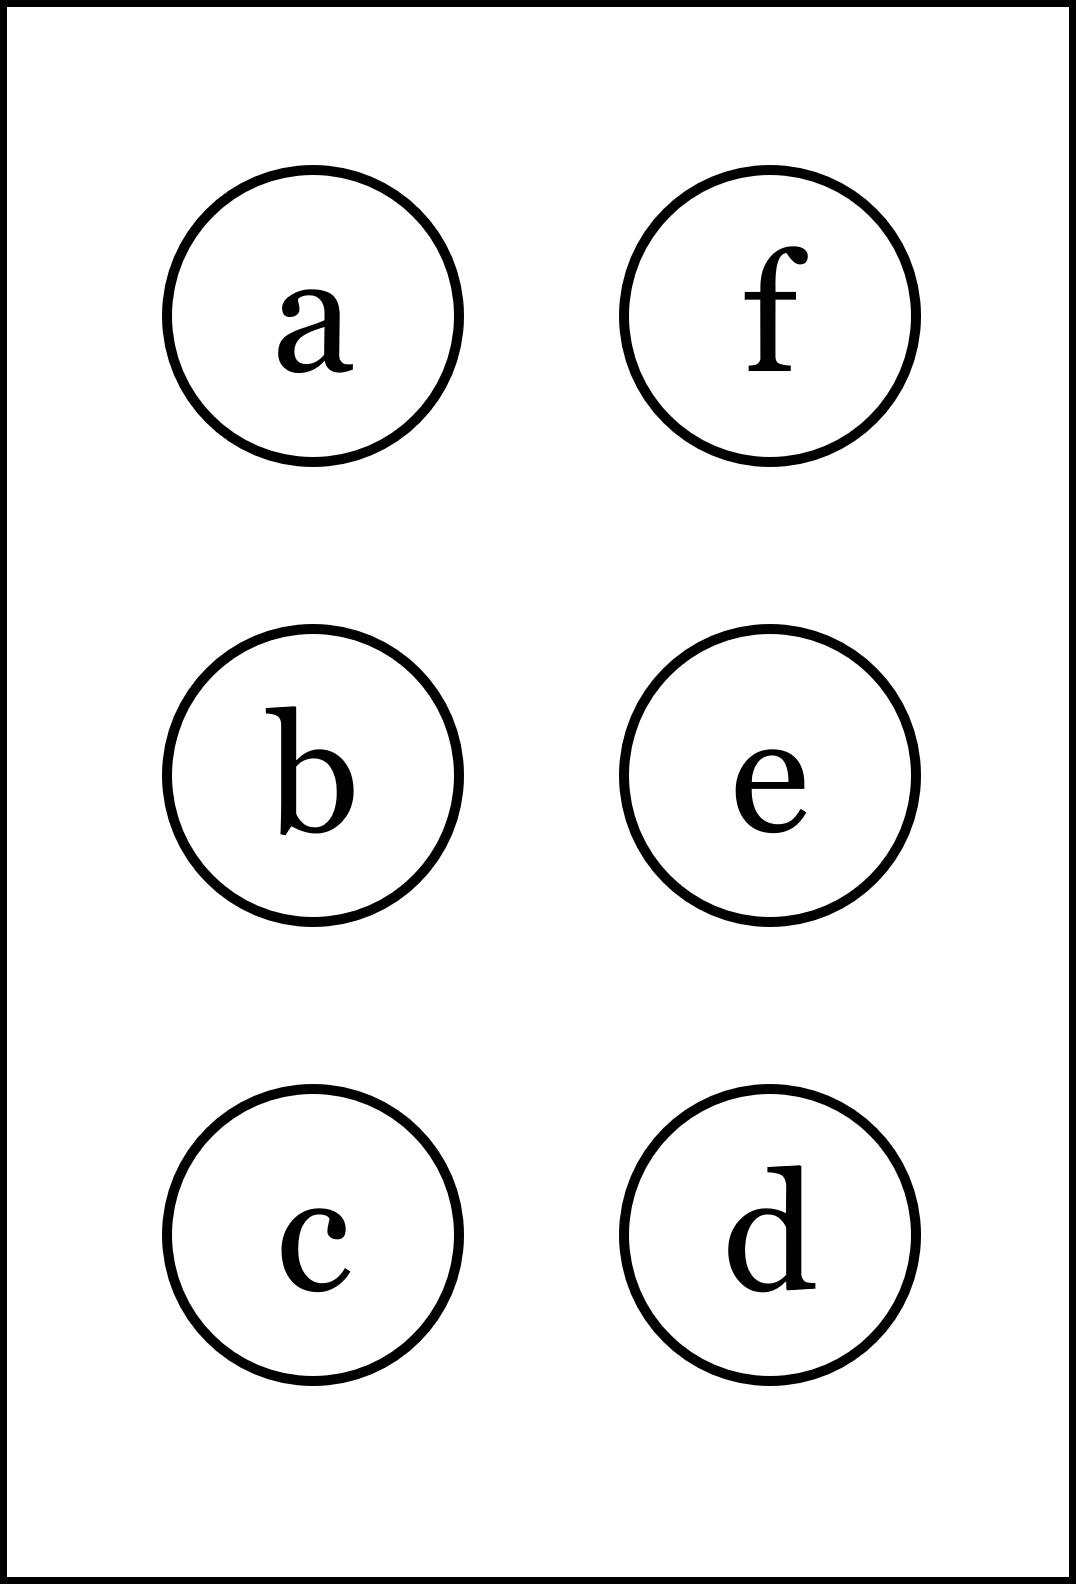
\includegraphics[height=40mm]{../images/braille.png}
{\small Písmeno Braillovej abecedy}
\end{center}
\end{minipage}
\end{center}
\end{minipage}
&
\begin{minipage}[c][104.5mm][t]{0.5\linewidth}
\begin{center}
\vspace{7mm}
{\huge Derivácie, skupina \textit{Alpha $\alpha$} -\romannumeral2}\\[5mm]
\textit{Meno:}\phantom{xxxxxxxxxxxxxxxxxxxxxxxxxxxxxxxxxxxxxxxxxxxxxxxxxxxxxxxxxxxxxxxxx}\\[5mm]
\begin{minipage}{0.95\linewidth}
\begin{center}
\textbf{Vypočítej derivace.} Pokud se výsledky shodují s těmi za otazníky,\\tak napravo obarvi příslušející kroužek načerno. \textbf{Spolu odevzdejte výsledné slovo}.
\end{center}
\end{minipage}
\\[1mm]
\begin{minipage}{0.79\linewidth}
\begin{center}
\begin{varwidth}{\linewidth}
\begin{enumerate}
\normalsize
\item $4x^4-x^3+2x^2+2x-4$\quad \dotfill\; ???\;\dotfill \quad $16x^3-3x^2+4x+2$
\item $\cfrac{-5x^2+x+6}{-4x+6}$\quad \dotfill\; ???\;\dotfill \quad $\cfrac{20x^2-60x+30}{16x^2-48x+36}$
\item $\frac{8}{x}\sqrt{2x-1}$\quad \dotfill\; ???\;\dotfill \quad $\frac{-16x+16}{2x^2 \sqrt{\smash[b]{2x-1}}}$
\item $e^{3x^2+x+6}$\quad \dotfill\; ???\;\dotfill \quad $e^{3x^2+x+6}$
\item $\ln{\left(\frac{-2x-8}{-5x+1}\right)}$\quad \dotfill\; ???\;\dotfill \quad $\frac{-2}{-2x-8}+\frac{-5}{-5x+1}$
\item $\frac{e^{-x+5}}{5x+1}$\quad \dotfill\; ???\;\dotfill \quad $\frac{+5x-6}{(5x+1)^2}e^{-x+5}$
\end{enumerate}
\end{varwidth}
\end{center}
\end{minipage}
\begin{minipage}{0.20\linewidth}
\begin{center}
{\Huge\bfseries 2.} \\[2mm]
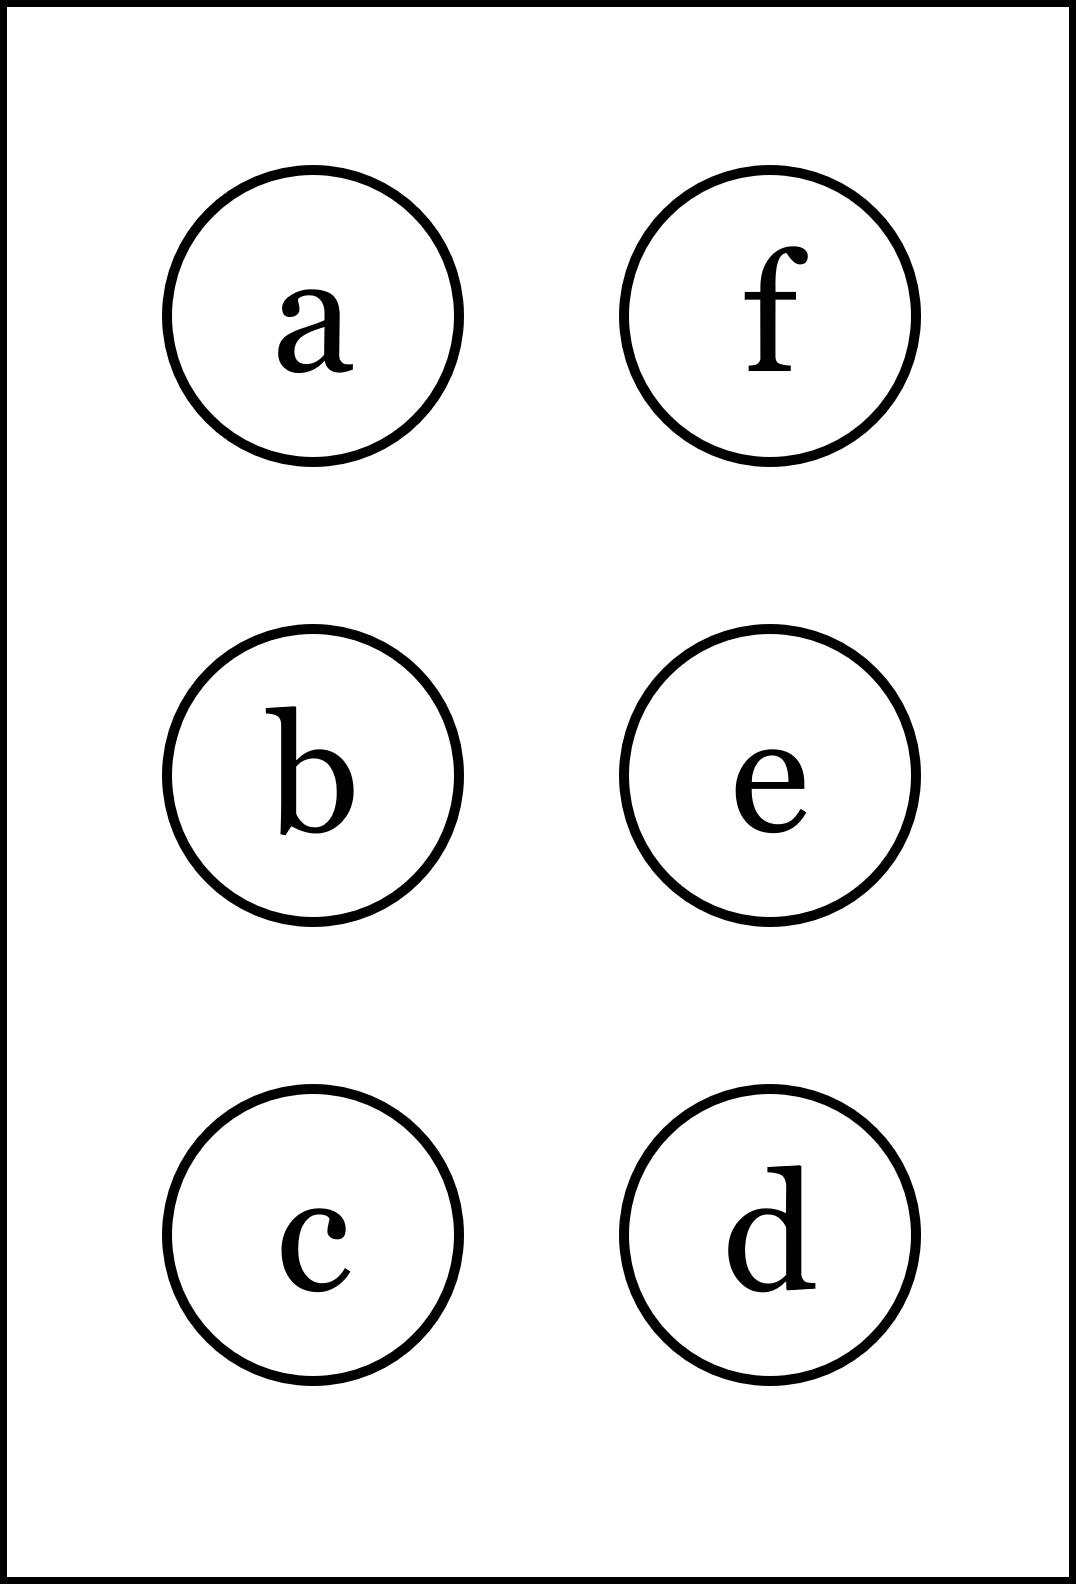
\includegraphics[height=40mm]{../images/braille.png}
{\small Písmeno Braillovej abecedy}
\end{center}
\end{minipage}
\end{center}
\end{minipage}
\\ \hdashline
\begin{minipage}[c][104.5mm][t]{0.5\linewidth}
\begin{center}
\vspace{7mm}
{\huge Derivácie, skupina \textit{Alpha $\alpha$} -\romannumeral3}\\[5mm]
\textit{Meno:}\phantom{xxxxxxxxxxxxxxxxxxxxxxxxxxxxxxxxxxxxxxxxxxxxxxxxxxxxxxxxxxxxxxxxx}\\[5mm]
\begin{minipage}{0.95\linewidth}
\begin{center}
\textbf{Vypočítej derivace.} Pokud se výsledky shodují s těmi za otazníky,\\tak napravo obarvi příslušející kroužek načerno. \textbf{Spolu odevzdejte výsledné slovo}.
\end{center}
\end{minipage}
\\[1mm]
\begin{minipage}{0.79\linewidth}
\begin{center}
\begin{varwidth}{\linewidth}
\begin{enumerate}
\normalsize
\item $-5x^4-4x^3+2x^2+8x-6$\quad \dotfill\; ???\;\dotfill \quad $-20x^3-12x^2+4x+8$
\item $\cfrac{-4x^2-3x-3}{-3x-4}$\quad \dotfill\; ???\;\dotfill \quad $\cfrac{12x^2-32x+3}{9x^2+24x+16}$
\item $\frac{4}{x}\sqrt{5x+1}$\quad \dotfill\; ???\;\dotfill \quad $\frac{-20x-8}{x^2 \sqrt{\smash[b]{5x+1}}}$
\item $e^{-7x^2-4x-4}$\quad \dotfill\; ???\;\dotfill \quad $e^{-7x^2-4x-4}$
\item $\ln{\left(\frac{x-4}{5x-5}\right)}$\quad \dotfill\; ???\;\dotfill \quad $\frac{1}{x-4}+\frac{5}{5x-5}$
\item $\frac{e^{3x-1}}{-6x-5}$\quad \dotfill\; ???\;\dotfill \quad $\frac{+18x-9}{(-6x-5)^2}e^{3x-1}$
\end{enumerate}
\end{varwidth}
\end{center}
\end{minipage}
\begin{minipage}{0.20\linewidth}
\begin{center}
{\Huge\bfseries 3.} \\[2mm]
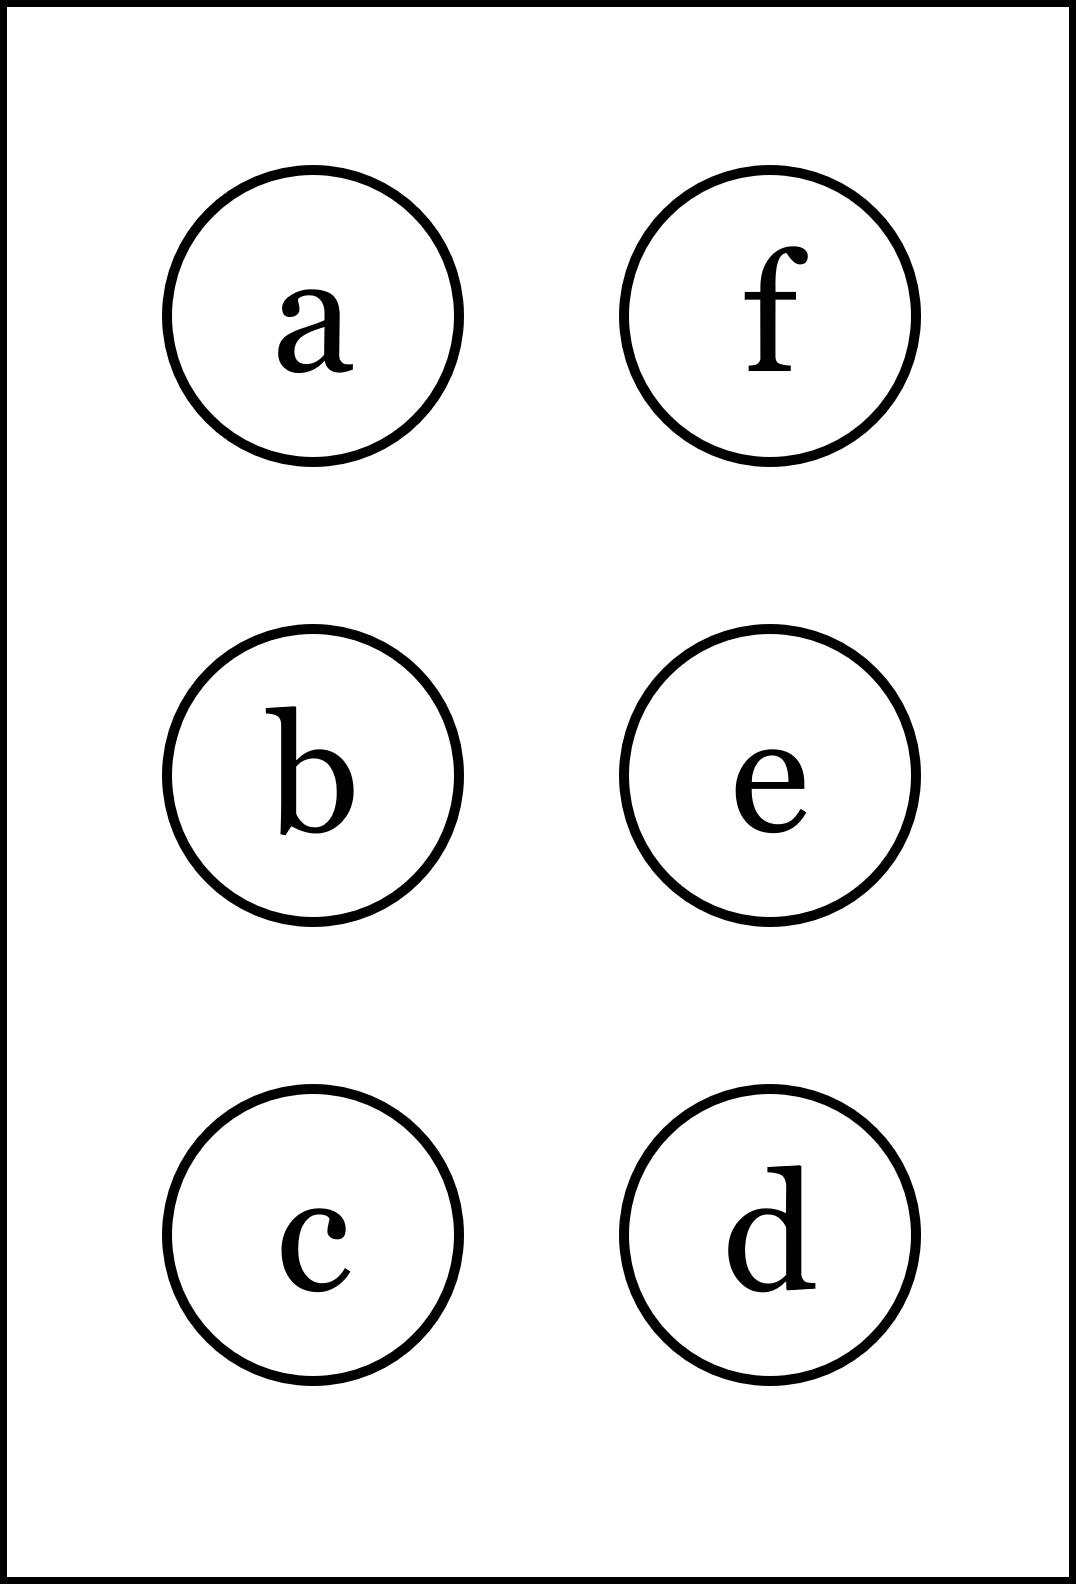
\includegraphics[height=40mm]{../images/braille.png}
{\small Písmeno Braillovej abecedy}
\end{center}
\end{minipage}
\end{center}
\end{minipage}
&
\begin{minipage}[c][104.5mm][t]{0.5\linewidth}
\begin{center}
\vspace{7mm}
{\huge Derivácie, skupina \textit{Alpha $\alpha$} -\romannumeral4}\\[5mm]
\textit{Meno:}\phantom{xxxxxxxxxxxxxxxxxxxxxxxxxxxxxxxxxxxxxxxxxxxxxxxxxxxxxxxxxxxxxxxxx}\\[5mm]
\begin{minipage}{0.95\linewidth}
\begin{center}
\textbf{Vypočítej derivace.} Pokud se výsledky shodují s těmi za otazníky,\\tak napravo obarvi příslušející kroužek načerno. \textbf{Spolu odevzdejte výsledné slovo}.
\end{center}
\end{minipage}
\\[1mm]
\begin{minipage}{0.79\linewidth}
\begin{center}
\begin{varwidth}{\linewidth}
\begin{enumerate}
\normalsize
\item $2x^4-8x^3+8x^2+6x-2$\quad \dotfill\; ???\;\dotfill \quad $8x^3-24x^2+16x+6$
\item $\cfrac{x^2-5x+3}{-x-1}$\quad \dotfill\; ???\;\dotfill \quad $\cfrac{-x^2+2x+8}{x^2+2x+1}$
\item $\frac{2}{x}\sqrt{x+3}$\quad \dotfill\; ???\;\dotfill \quad $\frac{-2x-12}{x^2 \sqrt{\smash[b]{x+3}}}$
\item $e^{-2x^2-2x-2}$\quad \dotfill\; ???\;\dotfill \quad $e^{-2x^2-2x-2}$
\item $\ln{\left(\frac{4x-3}{-9x+5}\right)}$\quad \dotfill\; ???\;\dotfill \quad $\frac{4}{4x-3}-\frac{-9}{-9x+5}$
\item $\frac{e^{-4x+2}}{-8x-1}$\quad \dotfill\; ???\;\dotfill \quad $\frac{32x+12}{(-8x-1)^2}e^{-4x+2}$
\end{enumerate}
\end{varwidth}
\end{center}
\end{minipage}
\begin{minipage}{0.20\linewidth}
\begin{center}
{\Huge\bfseries 4.} \\[2mm]
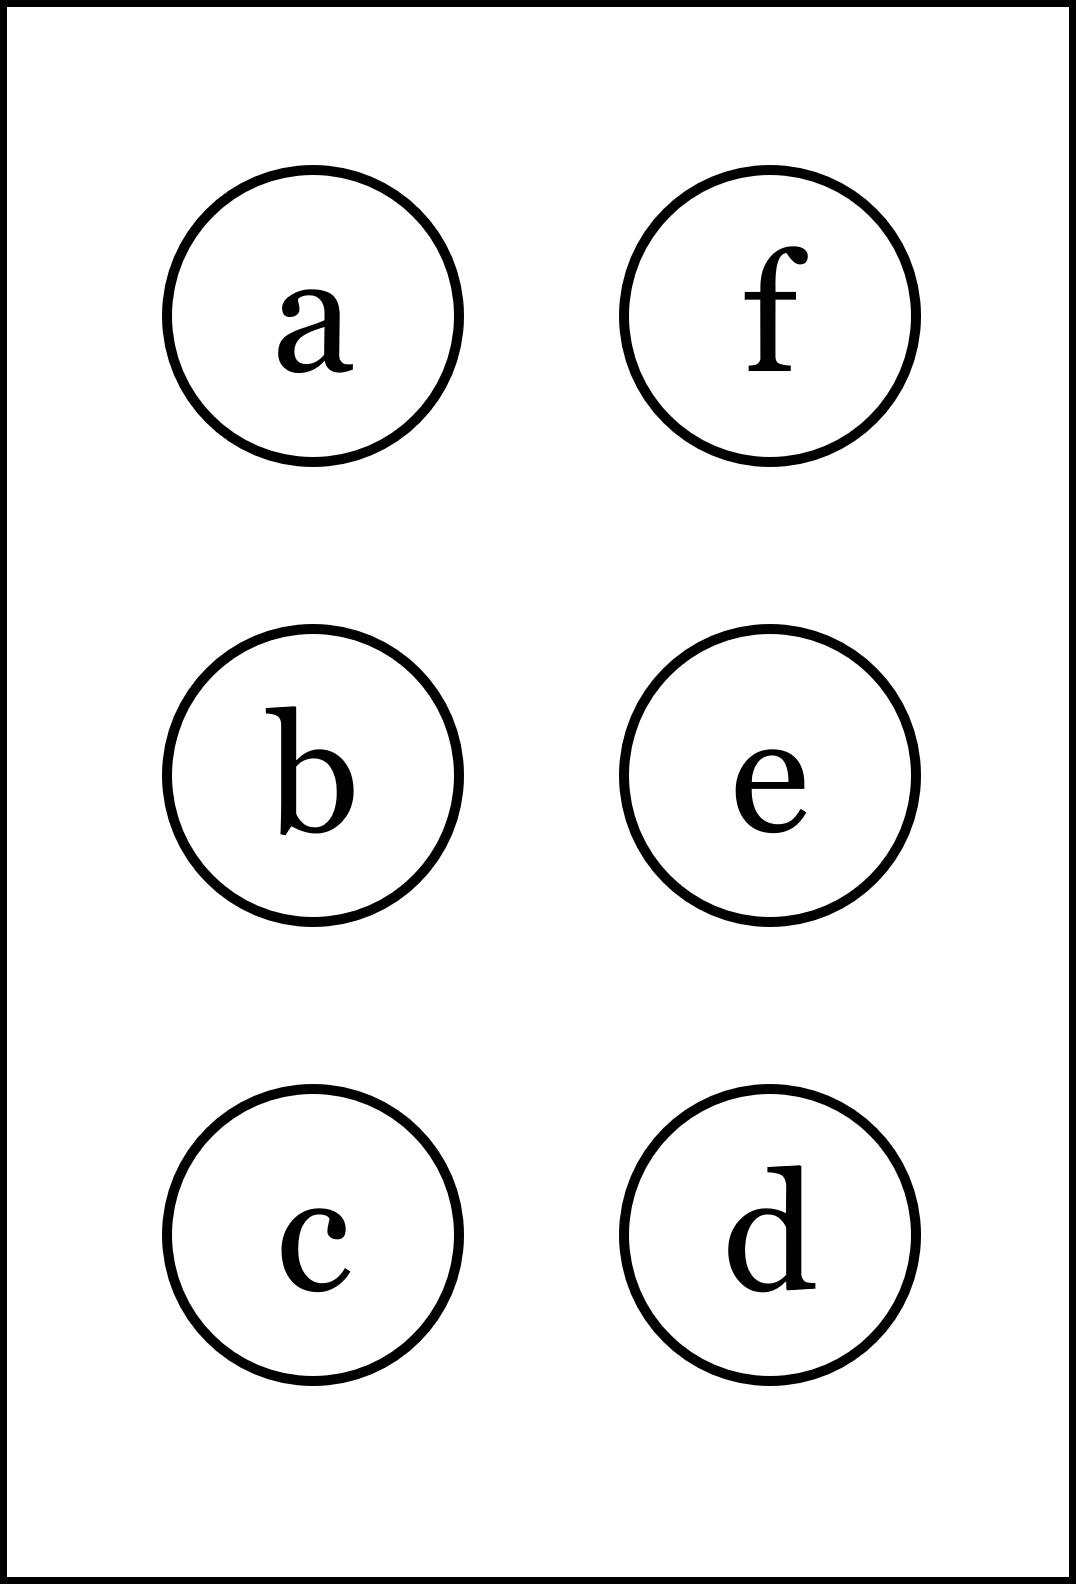
\includegraphics[height=40mm]{../images/braille.png}
{\small Písmeno Braillovej abecedy}
\end{center}
\end{minipage}
\end{center}
\end{minipage}
%
\end{tabular}
\newpage
\thispagestyle{empty}
\begin{tabular}{c:c}
\begin{minipage}[c][104.5mm][t]{0.5\linewidth}
\begin{center}
\vspace{7mm}
{\huge Derivácie, skupina \textit{Beta $\beta$} -\romannumeral1}\\[5mm]
\textit{Meno:}\phantom{xxxxxxxxxxxxxxxxxxxxxxxxxxxxxxxxxxxxxxxxxxxxxxxxxxxxxxxxxxxxxxxxx}\\[5mm]
\begin{minipage}{0.95\linewidth}
\begin{center}
\textbf{Vypočítej derivace.} Pokud se výsledky shodují s těmi za otazníky,\\tak napravo obarvi příslušející kroužek načerno. \textbf{Spolu odevzdejte výsledné slovo}.
\end{center}
\end{minipage}
\\[1mm]
\begin{minipage}{0.79\linewidth}
\begin{center}
\begin{varwidth}{\linewidth}
\begin{enumerate}
\normalsize
\item $-9x^4-3x^3+3x^2-3x+1$\quad \dotfill\; ???\;\dotfill \quad $-9x^3-3x^2+3x-3$
\item $\cfrac{-3x^2-6x+3}{3x+4}$\quad \dotfill\; ???\;\dotfill \quad $\cfrac{-9x^2-24x-33}{9x^2+24x+16}$
\item $\frac{2}{x}\sqrt{2x+7}$\quad \dotfill\; ???\;\dotfill \quad $\frac{-4x-28}{2x^2 \sqrt{\smash[b]{2x+7}}}$
\item $e^{9x^2+3x-3}$\quad \dotfill\; ???\;\dotfill \quad $(18x+3)e^{9x^2+3x-3}$
\item $\ln{\left(\frac{4x-1}{-7x+3}\right)}$\quad \dotfill\; ???\;\dotfill \quad $\frac{4}{4x-1}+\frac{-7}{-7x+3}$
\item $\frac{e^{-6x-4}}{8x-3}$\quad \dotfill\; ???\;\dotfill \quad $\frac{-48x+10}{(8x-3)^2}e^{-6x-4}$
\end{enumerate}
\end{varwidth}
\end{center}
\end{minipage}
\begin{minipage}{0.20\linewidth}
\begin{center}
{\Huge\bfseries 1.} \\[2mm]
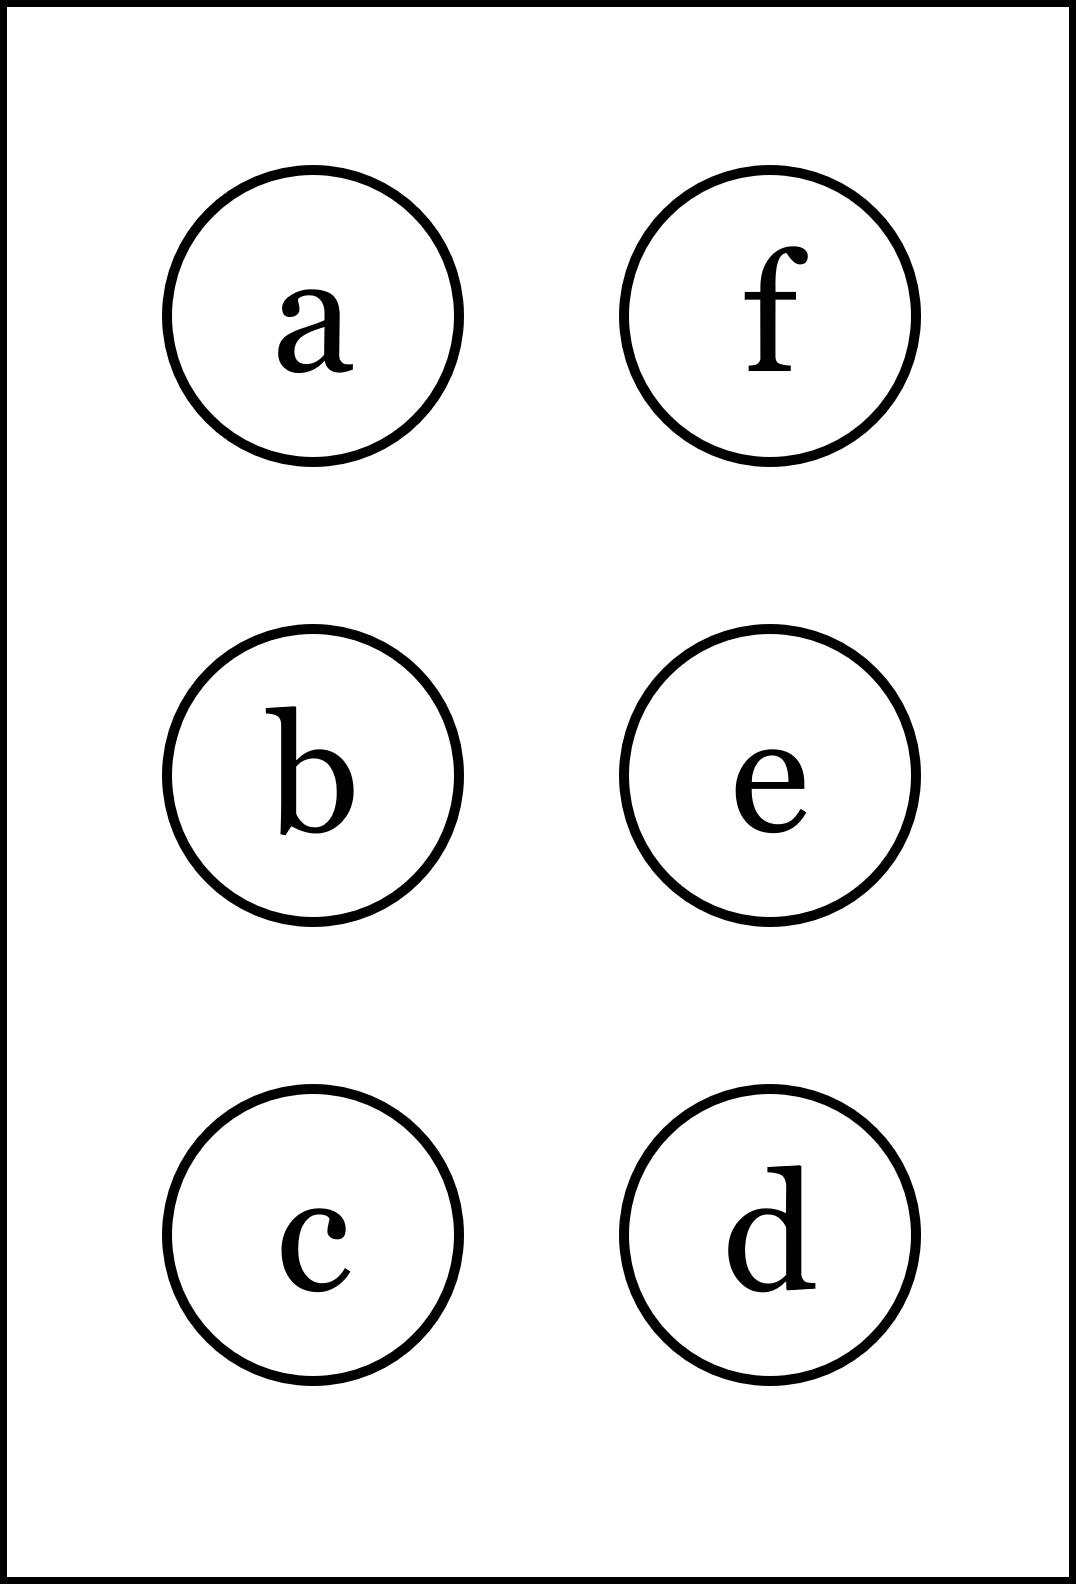
\includegraphics[height=40mm]{../images/braille.png}
{\small Písmeno Braillovej abecedy}
\end{center}
\end{minipage}
\end{center}
\end{minipage}
&
\begin{minipage}[c][104.5mm][t]{0.5\linewidth}
\begin{center}
\vspace{7mm}
{\huge Derivácie, skupina \textit{Beta $\beta$} -\romannumeral2}\\[5mm]
\textit{Meno:}\phantom{xxxxxxxxxxxxxxxxxxxxxxxxxxxxxxxxxxxxxxxxxxxxxxxxxxxxxxxxxxxxxxxxx}\\[5mm]
\begin{minipage}{0.95\linewidth}
\begin{center}
\textbf{Vypočítej derivace.} Pokud se výsledky shodují s těmi za otazníky,\\tak napravo obarvi příslušející kroužek načerno. \textbf{Spolu odevzdejte výsledné slovo}.
\end{center}
\end{minipage}
\\[1mm]
\begin{minipage}{0.79\linewidth}
\begin{center}
\begin{varwidth}{\linewidth}
\begin{enumerate}
\normalsize
\item $4x^4+2x^3-4x^2+6x+1$\quad \dotfill\; ???\;\dotfill \quad $16x^3+6x^2-8x+6$
\item $\cfrac{-4x^2-2x+2}{-3x-1}$\quad \dotfill\; ???\;\dotfill \quad $\cfrac{12x^2-8x+8}{9x^2+6x+1}$
\item $\frac{2}{x}\sqrt{-x+2}$\quad \dotfill\; ???\;\dotfill \quad $\frac{2x-8}{x^2 \sqrt{\smash[b]{-x+2}}}$
\item $e^{x^2-4x-3}$\quad \dotfill\; ???\;\dotfill \quad $(2x-4)e^{x^2-4x-3}$
\item $\ln{\left(\frac{7x+3}{6x+3}\right)}$\quad \dotfill\; ???\;\dotfill \quad $\frac{7}{7x+3}+\frac{6}{6x+3}$
\item $\frac{e^{6x-7}}{-x-6}$\quad \dotfill\; ???\;\dotfill \quad $\frac{+6x-35}{(-x-6)^2}e^{6x-7}$
\end{enumerate}
\end{varwidth}
\end{center}
\end{minipage}
\begin{minipage}{0.20\linewidth}
\begin{center}
{\Huge\bfseries 2.} \\[2mm]
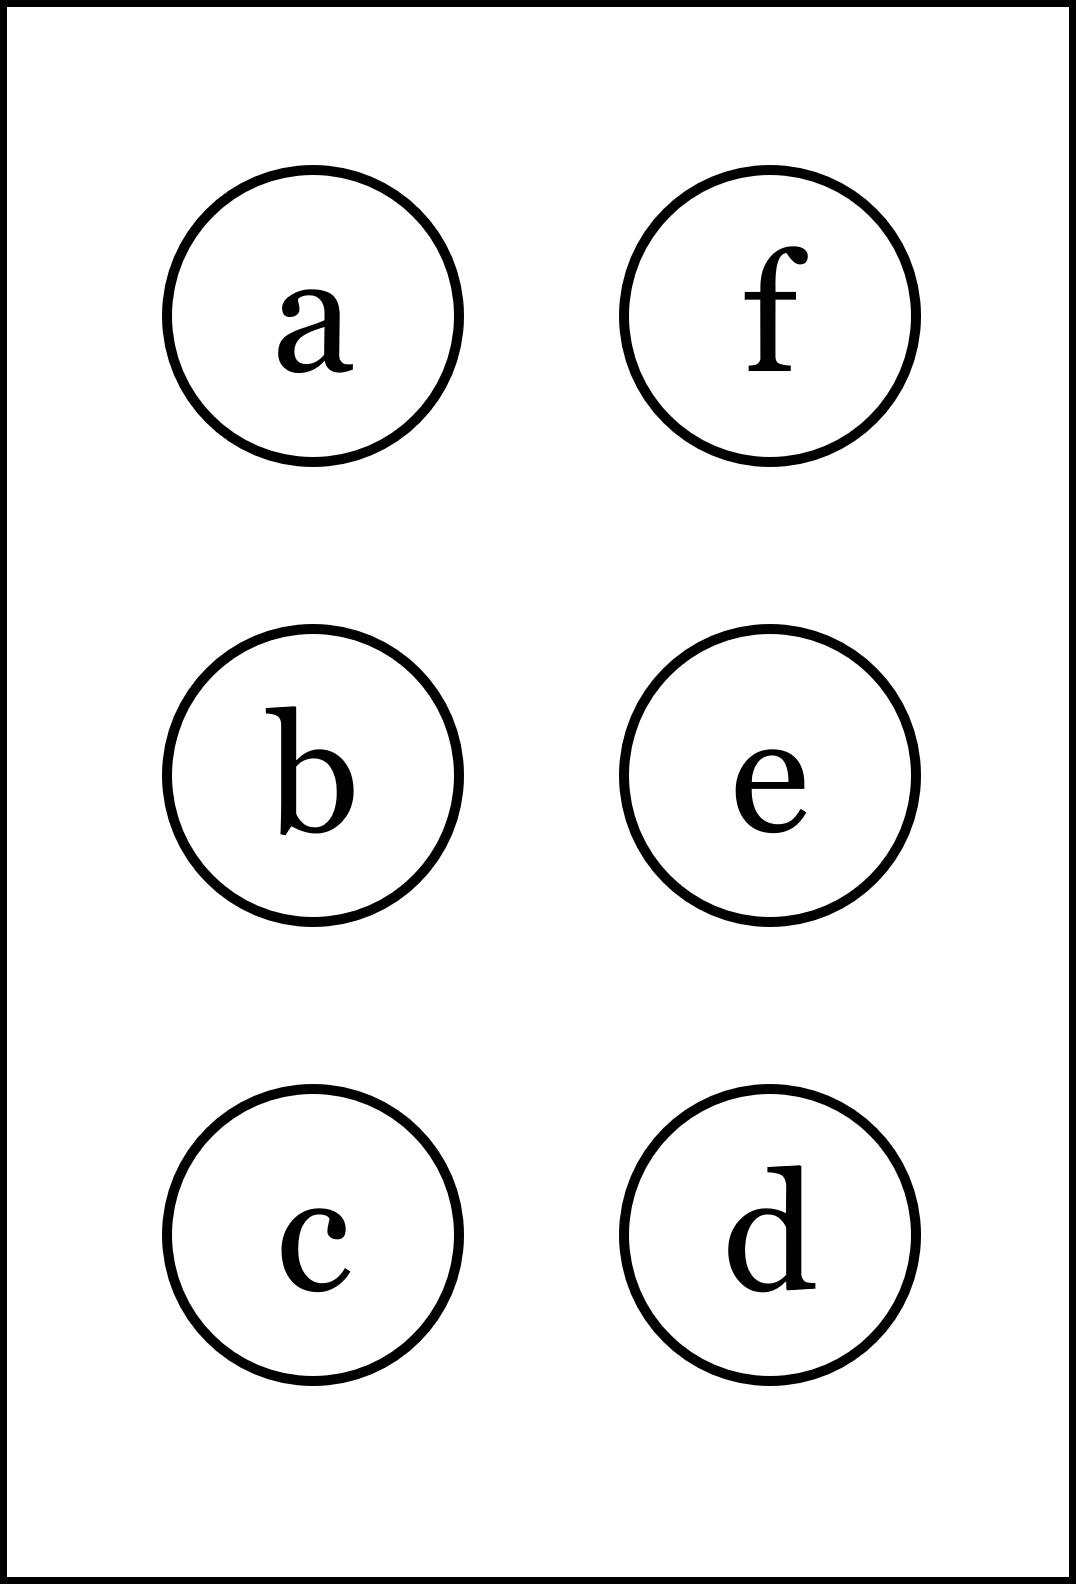
\includegraphics[height=40mm]{../images/braille.png}
{\small Písmeno Braillovej abecedy}
\end{center}
\end{minipage}
\end{center}
\end{minipage}
\\ \hdashline
\begin{minipage}[c][104.5mm][t]{0.5\linewidth}
\begin{center}
\vspace{7mm}
{\huge Derivácie, skupina \textit{Beta $\beta$} -\romannumeral3}\\[5mm]
\textit{Meno:}\phantom{xxxxxxxxxxxxxxxxxxxxxxxxxxxxxxxxxxxxxxxxxxxxxxxxxxxxxxxxxxxxxxxxx}\\[5mm]
\begin{minipage}{0.95\linewidth}
\begin{center}
\textbf{Vypočítej derivace.} Pokud se výsledky shodují s těmi za otazníky,\\tak napravo obarvi příslušející kroužek načerno. \textbf{Spolu odevzdejte výsledné slovo}.
\end{center}
\end{minipage}
\\[1mm]
\begin{minipage}{0.79\linewidth}
\begin{center}
\begin{varwidth}{\linewidth}
\begin{enumerate}
\normalsize
\item $-3x^4-2x^3+3x^2-8x-6$\quad \dotfill\; ???\;\dotfill \quad $-12x^3-6x^2+6x-8$
\item $\cfrac{-3x^2-x+6}{3x+2}$\quad \dotfill\; ???\;\dotfill \quad $\cfrac{-9x^2-12x-20}{9x^2+12x+4}$
\item $\frac{-2}{x}\sqrt{-5x-4}$\quad \dotfill\; ???\;\dotfill \quad $\frac{-10x-16}{x^2 \sqrt{\smash[b]{-5x-4}}}$
\item $e^{7x^2+4x-4}$\quad \dotfill\; ???\;\dotfill \quad $e^{7x^2+4x-4}$
\item $\ln{\left(\frac{2x-5}{-8x-5}\right)}$\quad \dotfill\; ???\;\dotfill \quad $\frac{2}{2x-5}+\frac{-8}{-8x-5}$
\item $\frac{e^{7x+4}}{x+7}$\quad \dotfill\; ???\;\dotfill \quad $\frac{-7x+48}{(x+7)^2}e^{7x+4}$
\end{enumerate}
\end{varwidth}
\end{center}
\end{minipage}
\begin{minipage}{0.20\linewidth}
\begin{center}
{\Huge\bfseries 3.} \\[2mm]
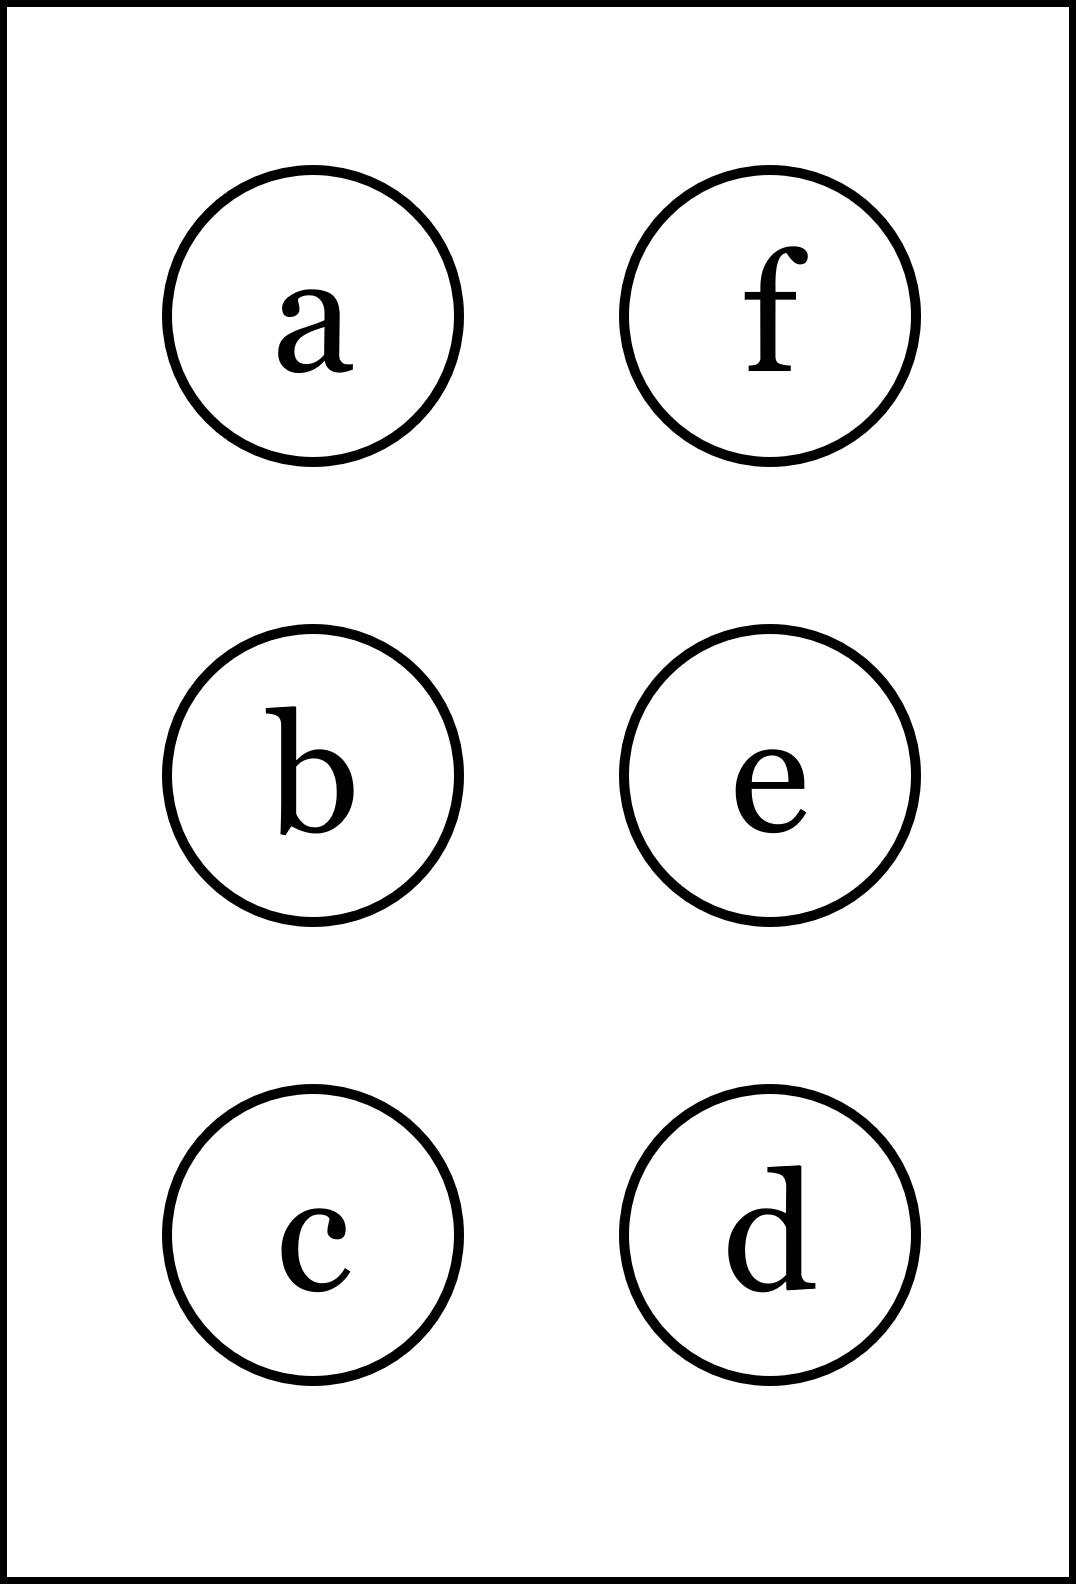
\includegraphics[height=40mm]{../images/braille.png}
{\small Písmeno Braillovej abecedy}
\end{center}
\end{minipage}
\end{center}
\end{minipage}
&
\begin{minipage}[c][104.5mm][t]{0.5\linewidth}
\begin{center}
\vspace{7mm}
{\huge Derivácie, skupina \textit{Beta $\beta$} -\romannumeral4}\\[5mm]
\textit{Meno:}\phantom{xxxxxxxxxxxxxxxxxxxxxxxxxxxxxxxxxxxxxxxxxxxxxxxxxxxxxxxxxxxxxxxxx}\\[5mm]
\begin{minipage}{0.95\linewidth}
\begin{center}
\textbf{Vypočítej derivace.} Pokud se výsledky shodují s těmi za otazníky,\\tak napravo obarvi příslušející kroužek načerno. \textbf{Spolu odevzdejte výsledné slovo}.
\end{center}
\end{minipage}
\\[1mm]
\begin{minipage}{0.79\linewidth}
\begin{center}
\begin{varwidth}{\linewidth}
\begin{enumerate}
\normalsize
\item $x^4-6x^3+6x^2+7x-5$\quad \dotfill\; ???\;\dotfill \quad $4x^3-18x^2+12x+7$
\item $\cfrac{-2x^2+5x-3}{-x+1}$\quad \dotfill\; ???\;\dotfill \quad $\cfrac{2x^2+4x+2}{x^2-2x+1}$
\item $\frac{3}{x}\sqrt{4x+7}$\quad \dotfill\; ???\;\dotfill \quad $\frac{-12x-42}{x^2 \sqrt{\smash[b]{4x+7}}}$
\item $e^{-5x^2+4x+4}$\quad \dotfill\; ???\;\dotfill \quad $e^{-5x^2+4x+4}$
\item $\ln{\left(\frac{4x+2}{-x-6}\right)}$\quad \dotfill\; ???\;\dotfill \quad $\frac{4}{4x+2}+\frac{-1}{-x-6}$
\item $\frac{e^{5x-4}}{-x+3}$\quad \dotfill\; ???\;\dotfill \quad $\frac{+5x+16}{(-x+3)^2}e^{5x-4}$
\end{enumerate}
\end{varwidth}
\end{center}
\end{minipage}
\begin{minipage}{0.20\linewidth}
\begin{center}
{\Huge\bfseries 4.} \\[2mm]
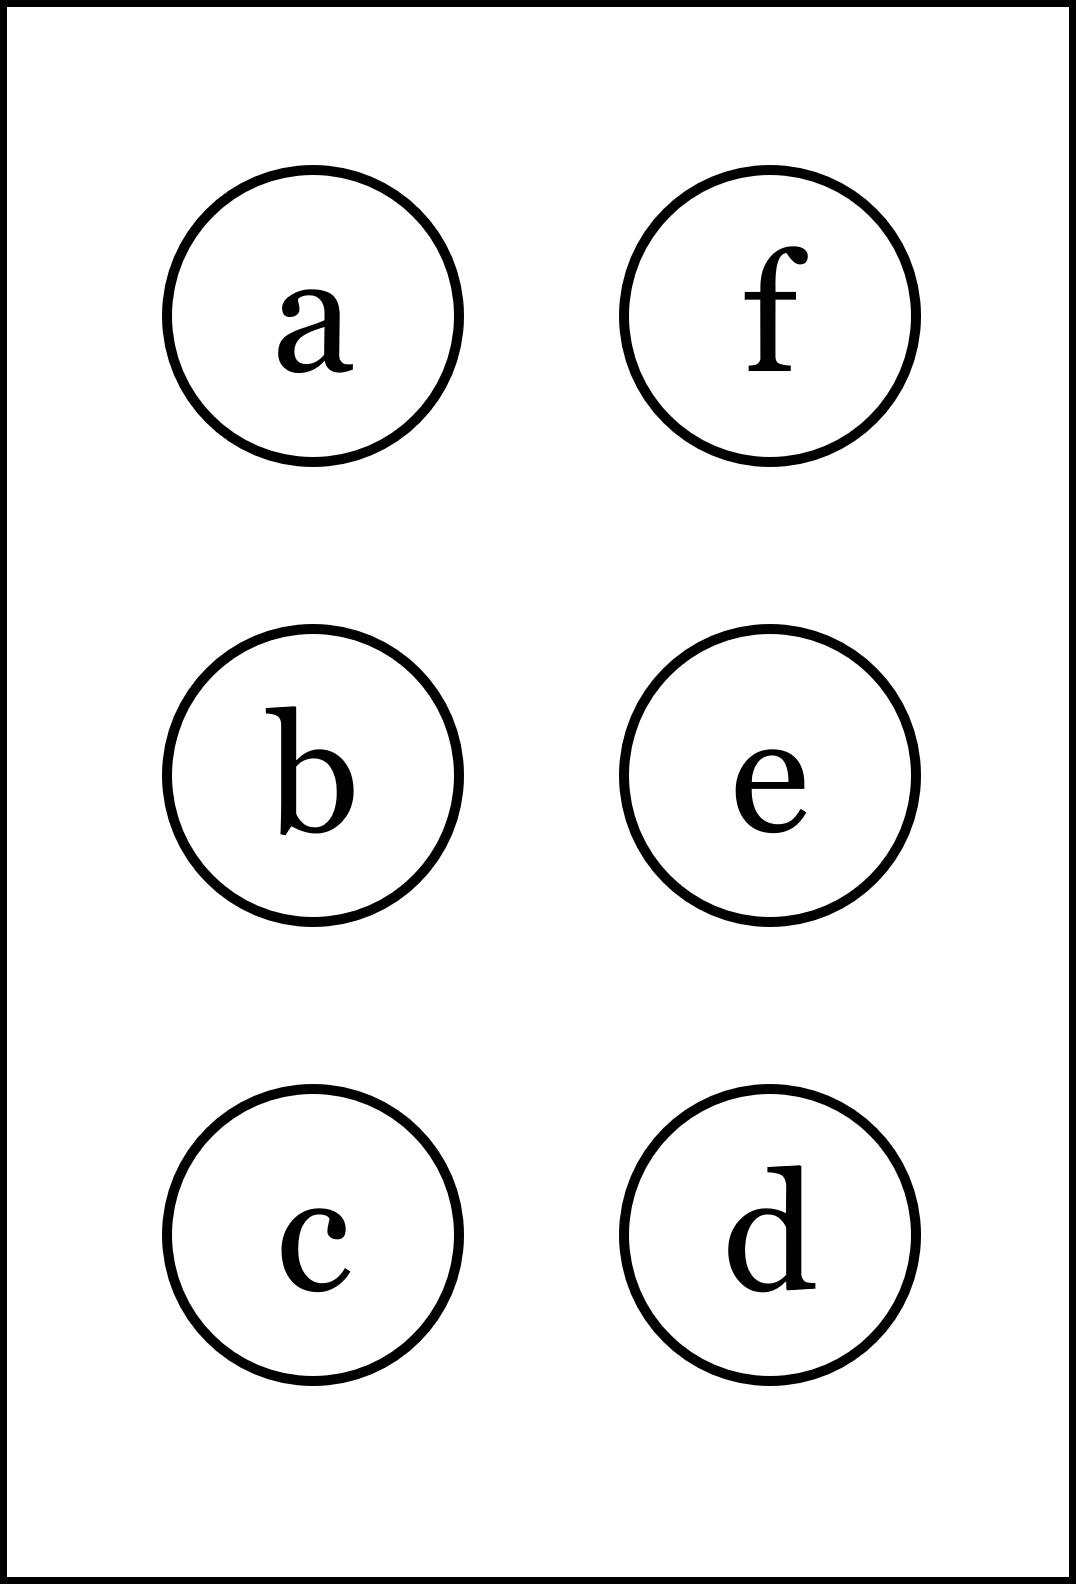
\includegraphics[height=40mm]{../images/braille.png}
{\small Písmeno Braillovej abecedy}
\end{center}
\end{minipage}
\end{center}
\end{minipage}
%
\end{tabular}
\newpage
\thispagestyle{empty}
\begin{tabular}{c:c}
\begin{minipage}[c][104.5mm][t]{0.5\linewidth}
\begin{center}
\vspace{7mm}
{\huge Derivácie, skupina \textit{Gamma $\gamma$} -\romannumeral1}\\[5mm]
\textit{Meno:}\phantom{xxxxxxxxxxxxxxxxxxxxxxxxxxxxxxxxxxxxxxxxxxxxxxxxxxxxxxxxxxxxxxxxx}\\[5mm]
\begin{minipage}{0.95\linewidth}
\begin{center}
\textbf{Vypočítej derivace.} Pokud se výsledky shodují s těmi za otazníky,\\tak napravo obarvi příslušející kroužek načerno. \textbf{Spolu odevzdejte výsledné slovo}.
\end{center}
\end{minipage}
\\[1mm]
\begin{minipage}{0.79\linewidth}
\begin{center}
\begin{varwidth}{\linewidth}
\begin{enumerate}
\normalsize
\item $2x^4+7x^3-3x^2+8x-5$\quad \dotfill\; ???\;\dotfill \quad $8x^3+21x^2-6x+8$
\item $\cfrac{5x^2-2x-5}{6x-6}$\quad \dotfill\; ???\;\dotfill \quad $\cfrac{30x^2+60x+42}{36x^2-72x+36}$
\item $\frac{-4}{x}\sqrt{3x-2}$\quad \dotfill\; ???\;\dotfill \quad $\frac{12x-16}{2x^2 \sqrt{\smash[b]{3x-2}}}$
\item $e^{4x^2+x+1}$\quad \dotfill\; ???\;\dotfill \quad $e^{4x^2+x+1}$
\item $\ln{\left(\frac{-8x-8}{x-1}\right)}$\quad \dotfill\; ???\;\dotfill \quad $\frac{-8}{-8x-8}-\frac{1}{x-1}$
\item $\frac{e^{-3x+7}}{6x-5}$\quad \dotfill\; ???\;\dotfill \quad $\frac{+18x+9}{(6x-5)^2}e^{-3x+7}$
\end{enumerate}
\end{varwidth}
\end{center}
\end{minipage}
\begin{minipage}{0.20\linewidth}
\begin{center}
{\Huge\bfseries 1.} \\[2mm]
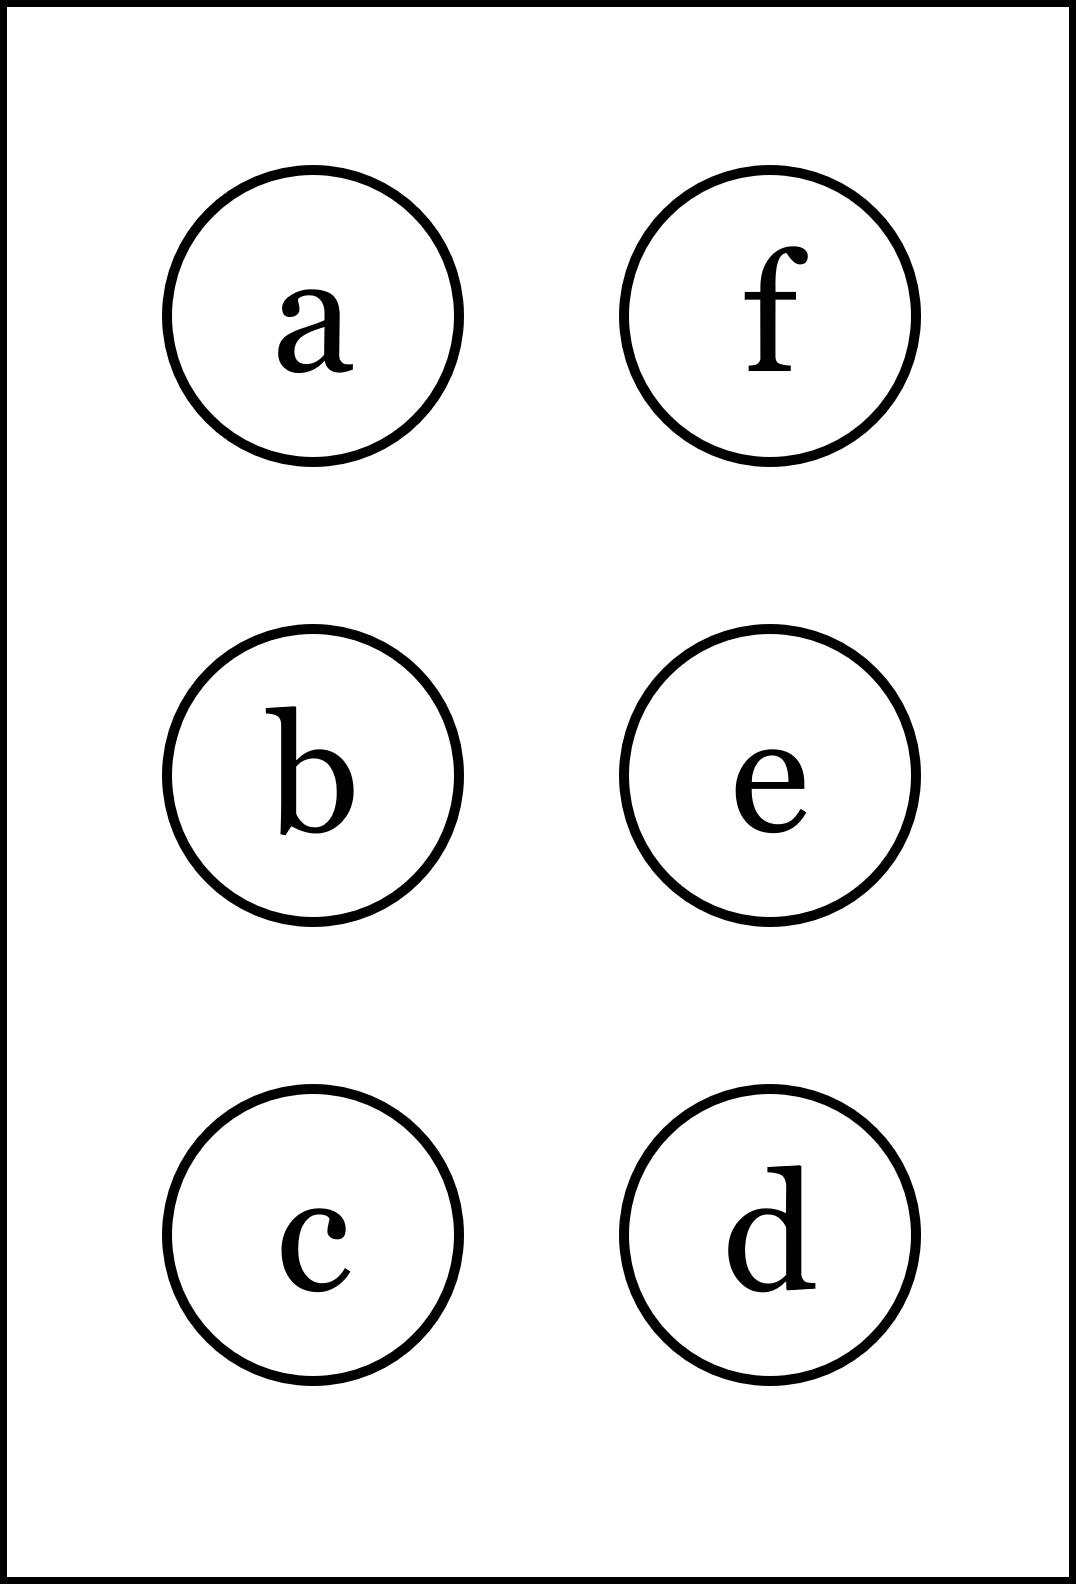
\includegraphics[height=40mm]{../images/braille.png}
{\small Písmeno Braillovej abecedy}
\end{center}
\end{minipage}
\end{center}
\end{minipage}
&
\begin{minipage}[c][104.5mm][t]{0.5\linewidth}
\begin{center}
\vspace{7mm}
{\huge Derivácie, skupina \textit{Gamma $\gamma$} -\romannumeral2}\\[5mm]
\textit{Meno:}\phantom{xxxxxxxxxxxxxxxxxxxxxxxxxxxxxxxxxxxxxxxxxxxxxxxxxxxxxxxxxxxxxxxxx}\\[5mm]
\begin{minipage}{0.95\linewidth}
\begin{center}
\textbf{Vypočítej derivace.} Pokud se výsledky shodují s těmi za otazníky,\\tak napravo obarvi příslušející kroužek načerno. \textbf{Spolu odevzdejte výsledné slovo}.
\end{center}
\end{minipage}
\\[1mm]
\begin{minipage}{0.79\linewidth}
\begin{center}
\begin{varwidth}{\linewidth}
\begin{enumerate}
\normalsize
\item $-x^4-3x^3+2x^2+3x-2$\quad \dotfill\; ???\;\dotfill \quad $-4x^3-9x^2+4x+3$
\item $\cfrac{6x^2+4x-1}{-2x-1}$\quad \dotfill\; ???\;\dotfill \quad $\cfrac{-12x^2+12x-6}{4x^2+4x+1}$
\item $\frac{4}{x}\sqrt{5x-3}$\quad \dotfill\; ???\;\dotfill \quad $\frac{-20x+24}{2x^2 \sqrt{\smash[b]{5x-3}}}$
\item $e^{-3x^2+7x+9}$\quad \dotfill\; ???\;\dotfill \quad $e^{-3x^2+7x+9}$
\item $\ln{\left(\frac{-4x+3}{-4x+6}\right)}$\quad \dotfill\; ???\;\dotfill \quad $\frac{-4}{-4x+3}+\frac{-4}{-4x+6}$
\item $\frac{e^{-2x-3}}{9x-4}$\quad \dotfill\; ???\;\dotfill \quad $\frac{+18x-1}{(9x-4)^2}e^{-2x-3}$
\end{enumerate}
\end{varwidth}
\end{center}
\end{minipage}
\begin{minipage}{0.20\linewidth}
\begin{center}
{\Huge\bfseries 2.} \\[2mm]
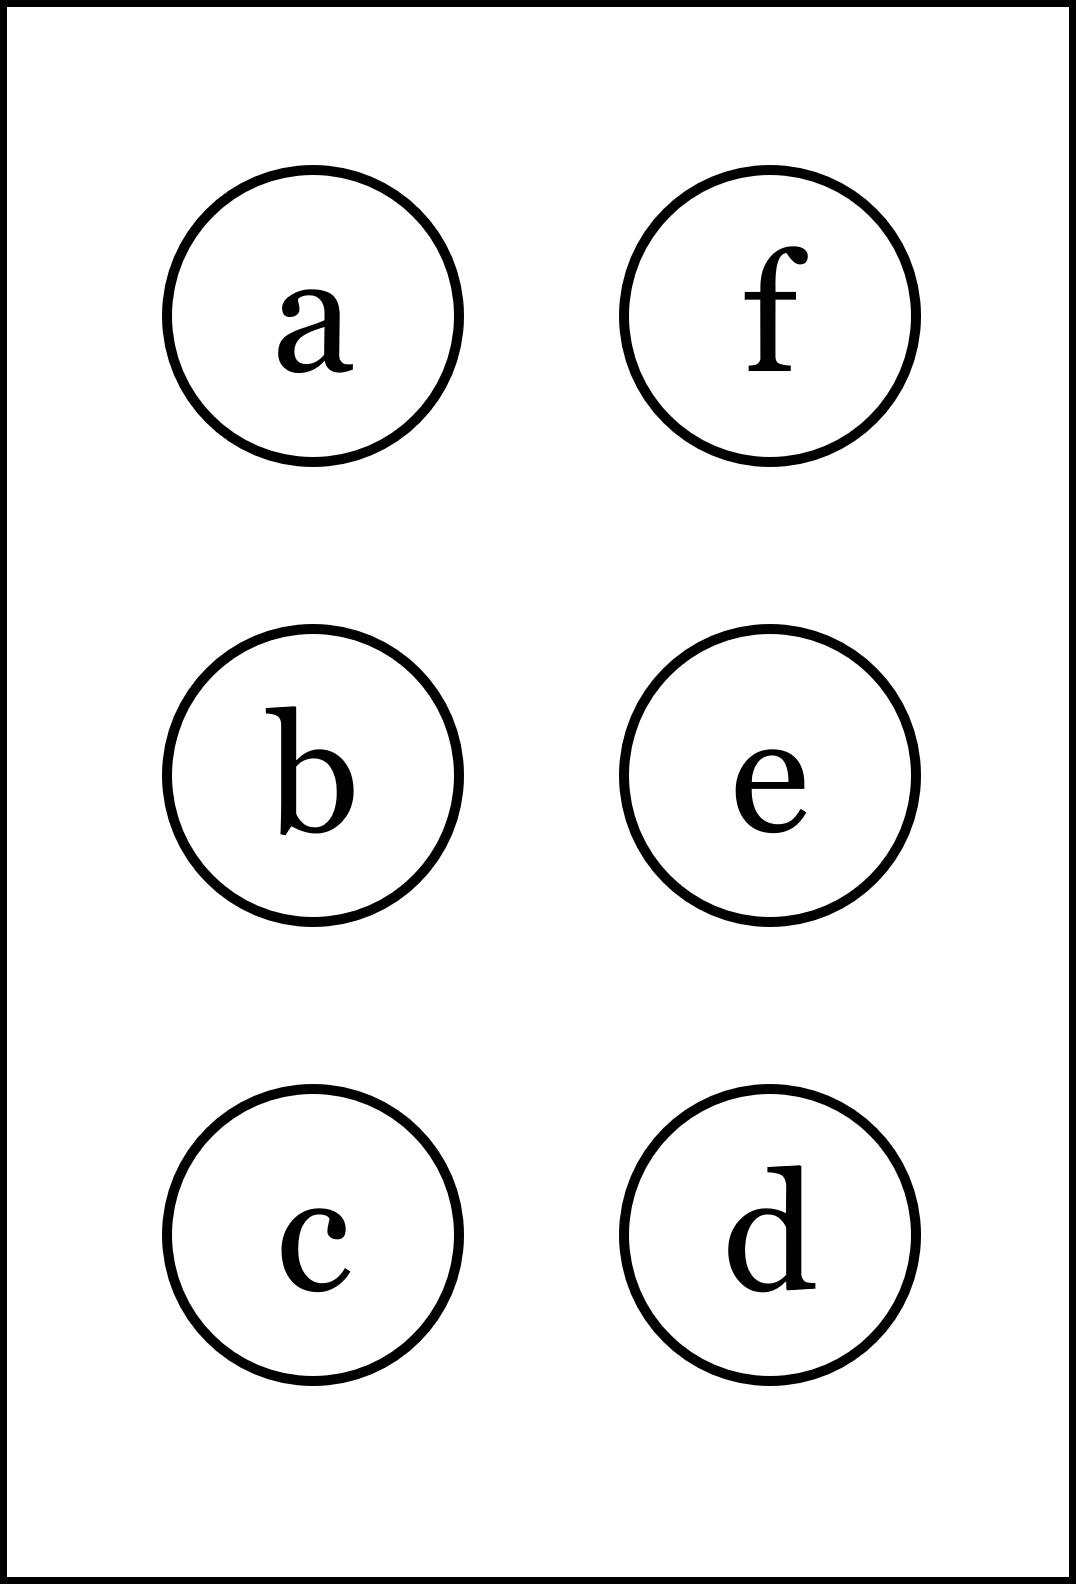
\includegraphics[height=40mm]{../images/braille.png}
{\small Písmeno Braillovej abecedy}
\end{center}
\end{minipage}
\end{center}
\end{minipage}
\\ \hdashline
\begin{minipage}[c][104.5mm][t]{0.5\linewidth}
\begin{center}
\vspace{7mm}
{\huge Derivácie, skupina \textit{Gamma $\gamma$} -\romannumeral3}\\[5mm]
\textit{Meno:}\phantom{xxxxxxxxxxxxxxxxxxxxxxxxxxxxxxxxxxxxxxxxxxxxxxxxxxxxxxxxxxxxxxxxx}\\[5mm]
\begin{minipage}{0.95\linewidth}
\begin{center}
\textbf{Vypočítej derivace.} Pokud se výsledky shodují s těmi za otazníky,\\tak napravo obarvi příslušející kroužek načerno. \textbf{Spolu odevzdejte výsledné slovo}.
\end{center}
\end{minipage}
\\[1mm]
\begin{minipage}{0.79\linewidth}
\begin{center}
\begin{varwidth}{\linewidth}
\begin{enumerate}
\normalsize
\item $6x^4+5x^3+x^2-5x-3$\quad \dotfill\; ???\;\dotfill \quad $24x^3+15x^2+2x-5$
\item $\cfrac{3x^2+x-1}{-2x+1}$\quad \dotfill\; ???\;\dotfill \quad $\cfrac{-6x^2-6x-1}{4x^2-4x+1}$
\item $\frac{8}{x}\sqrt{-3x-2}$\quad \dotfill\; ???\;\dotfill \quad $\frac{24x+32}{2x^2 \sqrt{\smash[b]{-3x-2}}}$
\item $e^{3x^2-5x-1}$\quad \dotfill\; ???\;\dotfill \quad $e^{3x^2-5x-1}$
\item $\ln{\left(\frac{7x-5}{2x+7}\right)}$\quad \dotfill\; ???\;\dotfill \quad $\frac{7}{7x-5}-\frac{2}{2x+7}$
\item $\frac{e^{-x-1}}{3x+4}$\quad \dotfill\; ???\;\dotfill \quad $\frac{-3x-7}{(3x+4)^2}e^{-x-1}$
\end{enumerate}
\end{varwidth}
\end{center}
\end{minipage}
\begin{minipage}{0.20\linewidth}
\begin{center}
{\Huge\bfseries 3.} \\[2mm]
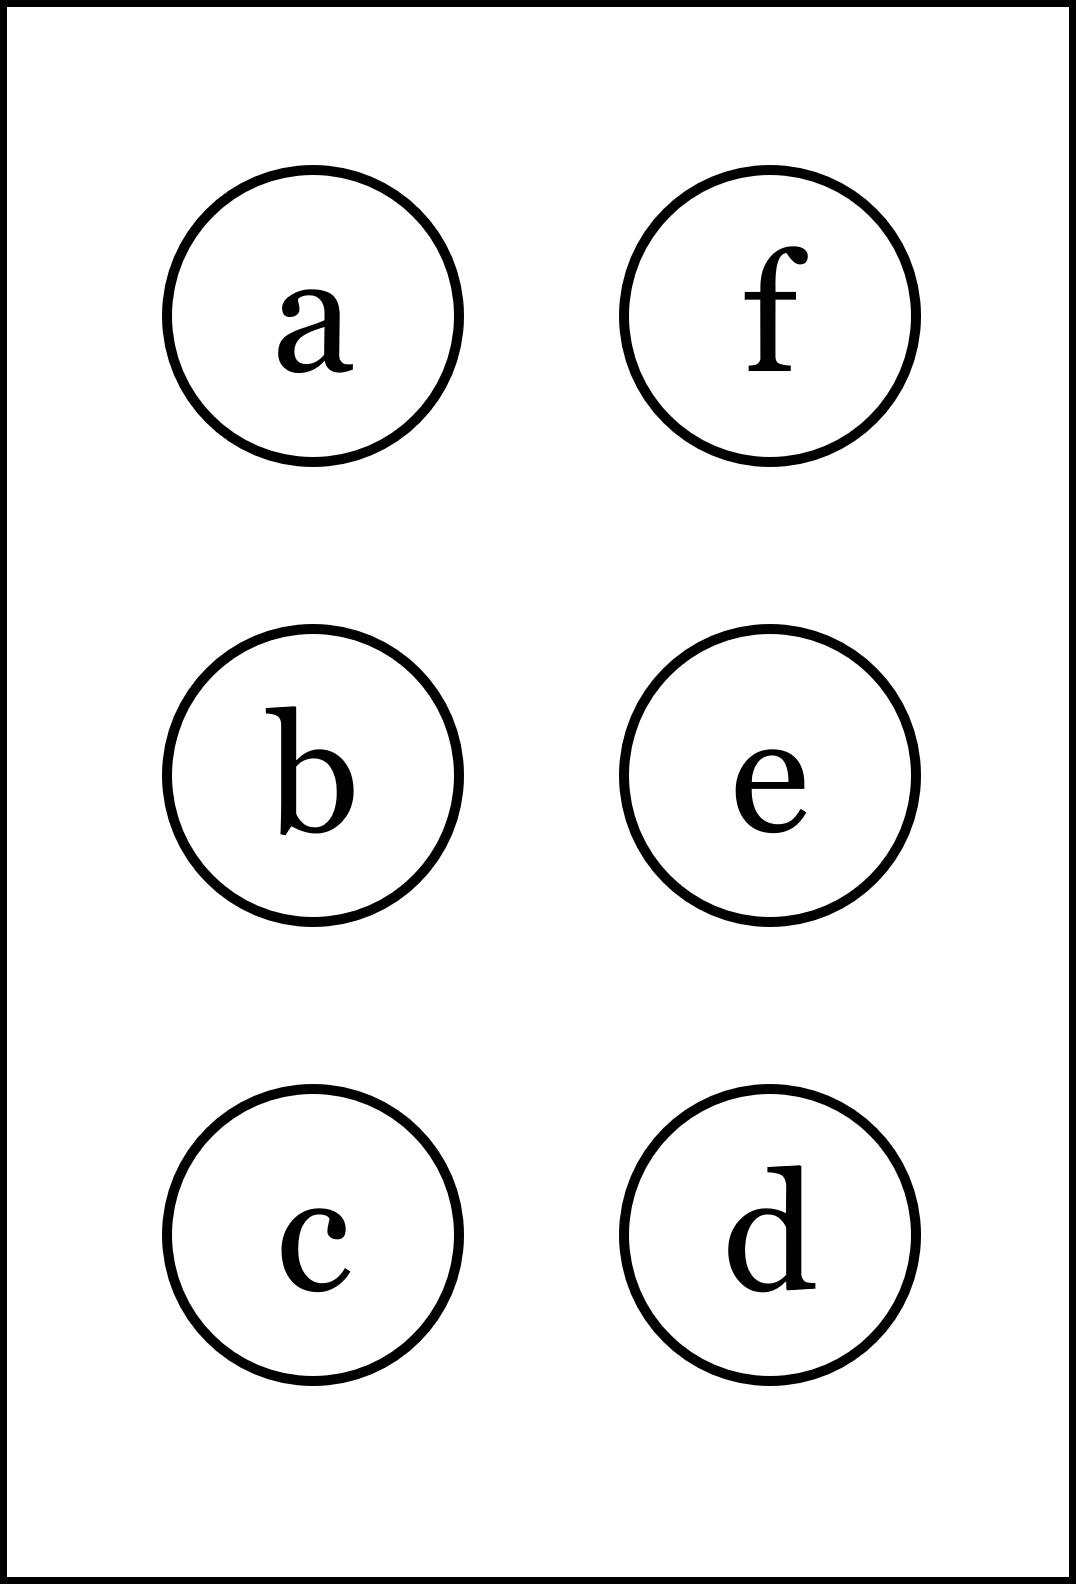
\includegraphics[height=40mm]{../images/braille.png}
{\small Písmeno Braillovej abecedy}
\end{center}
\end{minipage}
\end{center}
\end{minipage}
&
\begin{minipage}[c][104.5mm][t]{0.5\linewidth}
\begin{center}
\vspace{7mm}
{\huge Derivácie, skupina \textit{Gamma $\gamma$} -\romannumeral4}\\[5mm]
\textit{Meno:}\phantom{xxxxxxxxxxxxxxxxxxxxxxxxxxxxxxxxxxxxxxxxxxxxxxxxxxxxxxxxxxxxxxxxx}\\[5mm]
\begin{minipage}{0.95\linewidth}
\begin{center}
\textbf{Vypočítej derivace.} Pokud se výsledky shodují s těmi za otazníky,\\tak napravo obarvi příslušející kroužek načerno. \textbf{Spolu odevzdejte výsledné slovo}.
\end{center}
\end{minipage}
\\[1mm]
\begin{minipage}{0.79\linewidth}
\begin{center}
\begin{varwidth}{\linewidth}
\begin{enumerate}
\normalsize
\item $4x^4-6x^3-x^2-3x-3$\quad \dotfill\; ???\;\dotfill \quad $16x^3-18x^2-2x-3$
\item $\cfrac{4x^2-6x+3}{3x-1}$\quad \dotfill\; ???\;\dotfill \quad $\cfrac{12x^2+8x-3}{9x^2-6x+1}$
\item $\frac{-6}{x}\sqrt{3x-4}$\quad \dotfill\; ???\;\dotfill \quad $\frac{18x-48}{2x^2 \sqrt{\smash[b]{3x-4}}}$
\item $e^{9x^2+2x-7}$\quad \dotfill\; ???\;\dotfill \quad $e^{9x^2+2x-7}$
\item $\ln{\left(\frac{-6x+2}{5x+5}\right)}$\quad \dotfill\; ???\;\dotfill \quad $\frac{-6}{-6x+2}-\frac{5}{5x+5}$
\item $\frac{e^{-6x-4}}{-7x+2}$\quad \dotfill\; ???\;\dotfill \quad $\frac{-42x-5}{(-7x+2)^2}e^{-6x-4}$
\end{enumerate}
\end{varwidth}
\end{center}
\end{minipage}
\begin{minipage}{0.20\linewidth}
\begin{center}
{\Huge\bfseries 4.} \\[2mm]
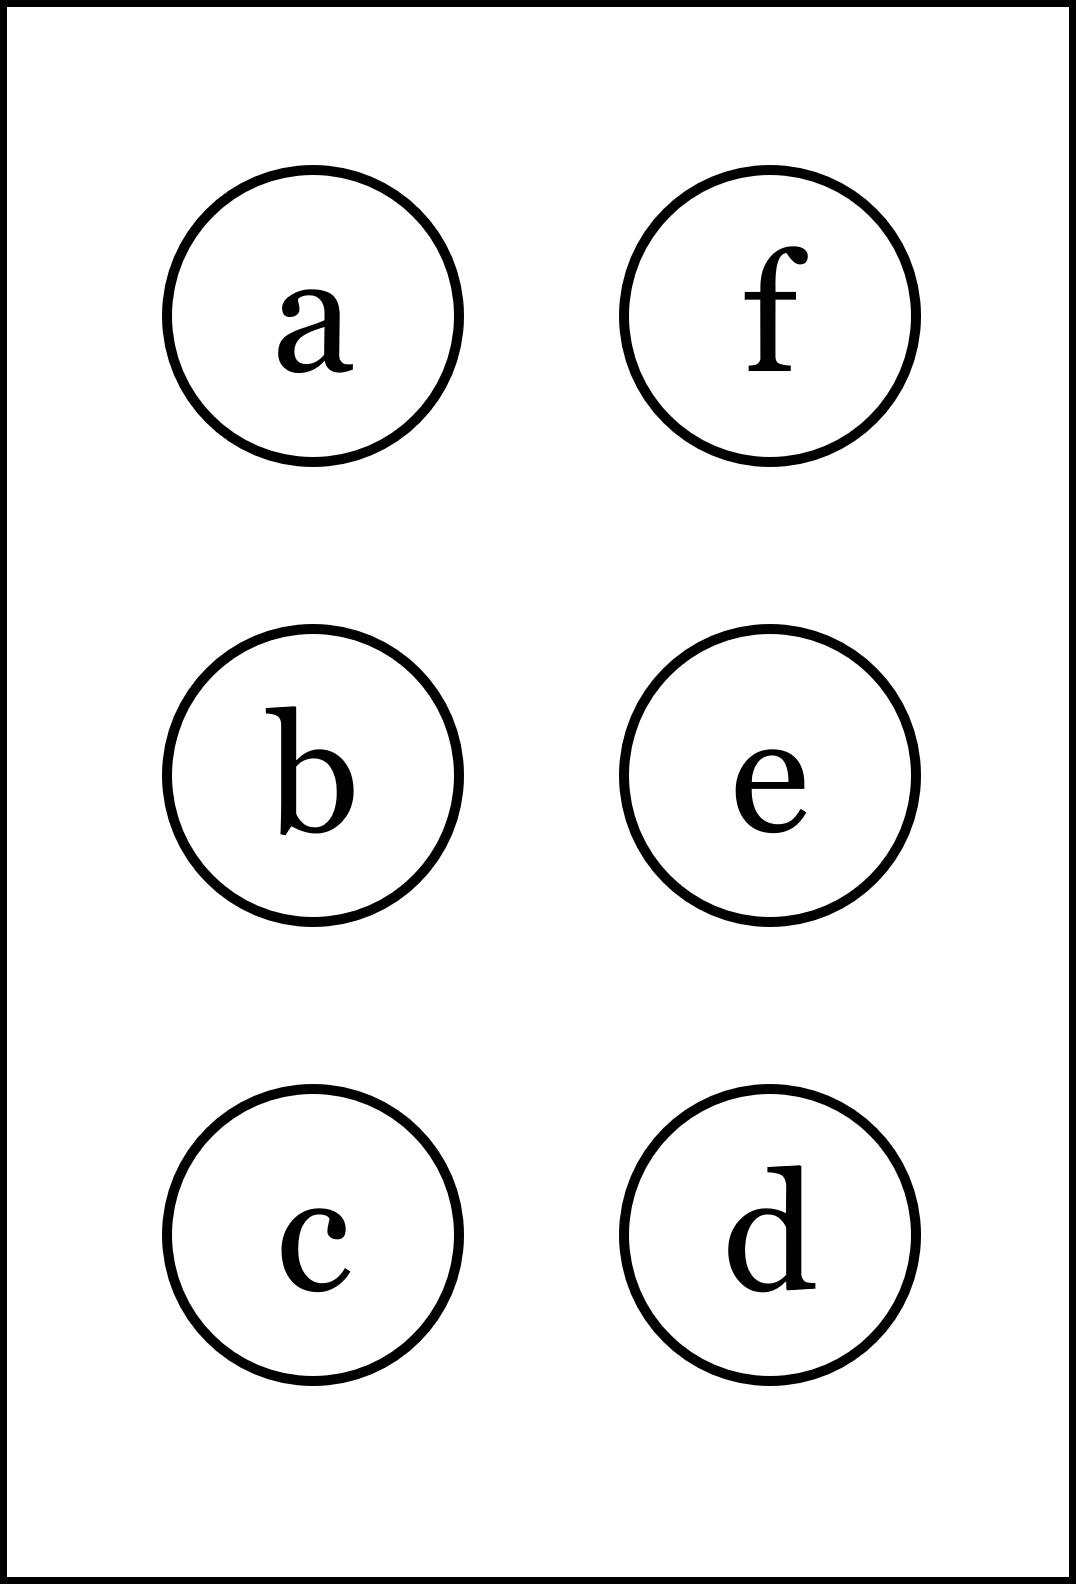
\includegraphics[height=40mm]{../images/braille.png}
{\small Písmeno Braillovej abecedy}
\end{center}
\end{minipage}
\end{center}
\end{minipage}
%
\end{tabular}
\newpage
\thispagestyle{empty}
\begin{tabular}{c:c}
\begin{minipage}[c][104.5mm][t]{0.5\linewidth}
\begin{center}
\vspace{7mm}
{\huge Derivácie, skupina \textit{Delta $\delta$} -\romannumeral1}\\[5mm]
\textit{Meno:}\phantom{xxxxxxxxxxxxxxxxxxxxxxxxxxxxxxxxxxxxxxxxxxxxxxxxxxxxxxxxxxxxxxxxx}\\[5mm]
\begin{minipage}{0.95\linewidth}
\begin{center}
\textbf{Vypočítej derivace.} Pokud se výsledky shodují s těmi za otazníky,\\tak napravo obarvi příslušející kroužek načerno. \textbf{Spolu odevzdejte výsledné slovo}.
\end{center}
\end{minipage}
\\[1mm]
\begin{minipage}{0.79\linewidth}
\begin{center}
\begin{varwidth}{\linewidth}
\begin{enumerate}
\normalsize
\item $5x^4-4x^3+x^2-6x+3$\quad \dotfill\; ???\;\dotfill \quad $20x^3-12x^2+2x-6$
\item $\cfrac{-3x^2+2x-2}{-4x-1}$\quad \dotfill\; ???\;\dotfill \quad $\cfrac{12x^2+6x-10}{16x^2+8x+1}$
\item $\frac{6}{x}\sqrt{-3x+1}$\quad \dotfill\; ???\;\dotfill \quad $\frac{18x-12}{2x^2 \sqrt{\smash[b]{-3x+1}}}$
\item $e^{2x^2+2x-9}$\quad \dotfill\; ???\;\dotfill \quad $e^{2x^2+2x-9}$
\item $\ln{\left(\frac{-4x-5}{2x+3}\right)}$\quad \dotfill\; ???\;\dotfill \quad $\frac{-4}{-4x-5}-\frac{2}{2x+3}$
\item $\frac{e^{3x-4}}{x-6}$\quad \dotfill\; ???\;\dotfill \quad $\frac{-3x-19}{(x-6)^2}e^{3x-4}$
\end{enumerate}
\end{varwidth}
\end{center}
\end{minipage}
\begin{minipage}{0.20\linewidth}
\begin{center}
{\Huge\bfseries 1.} \\[2mm]
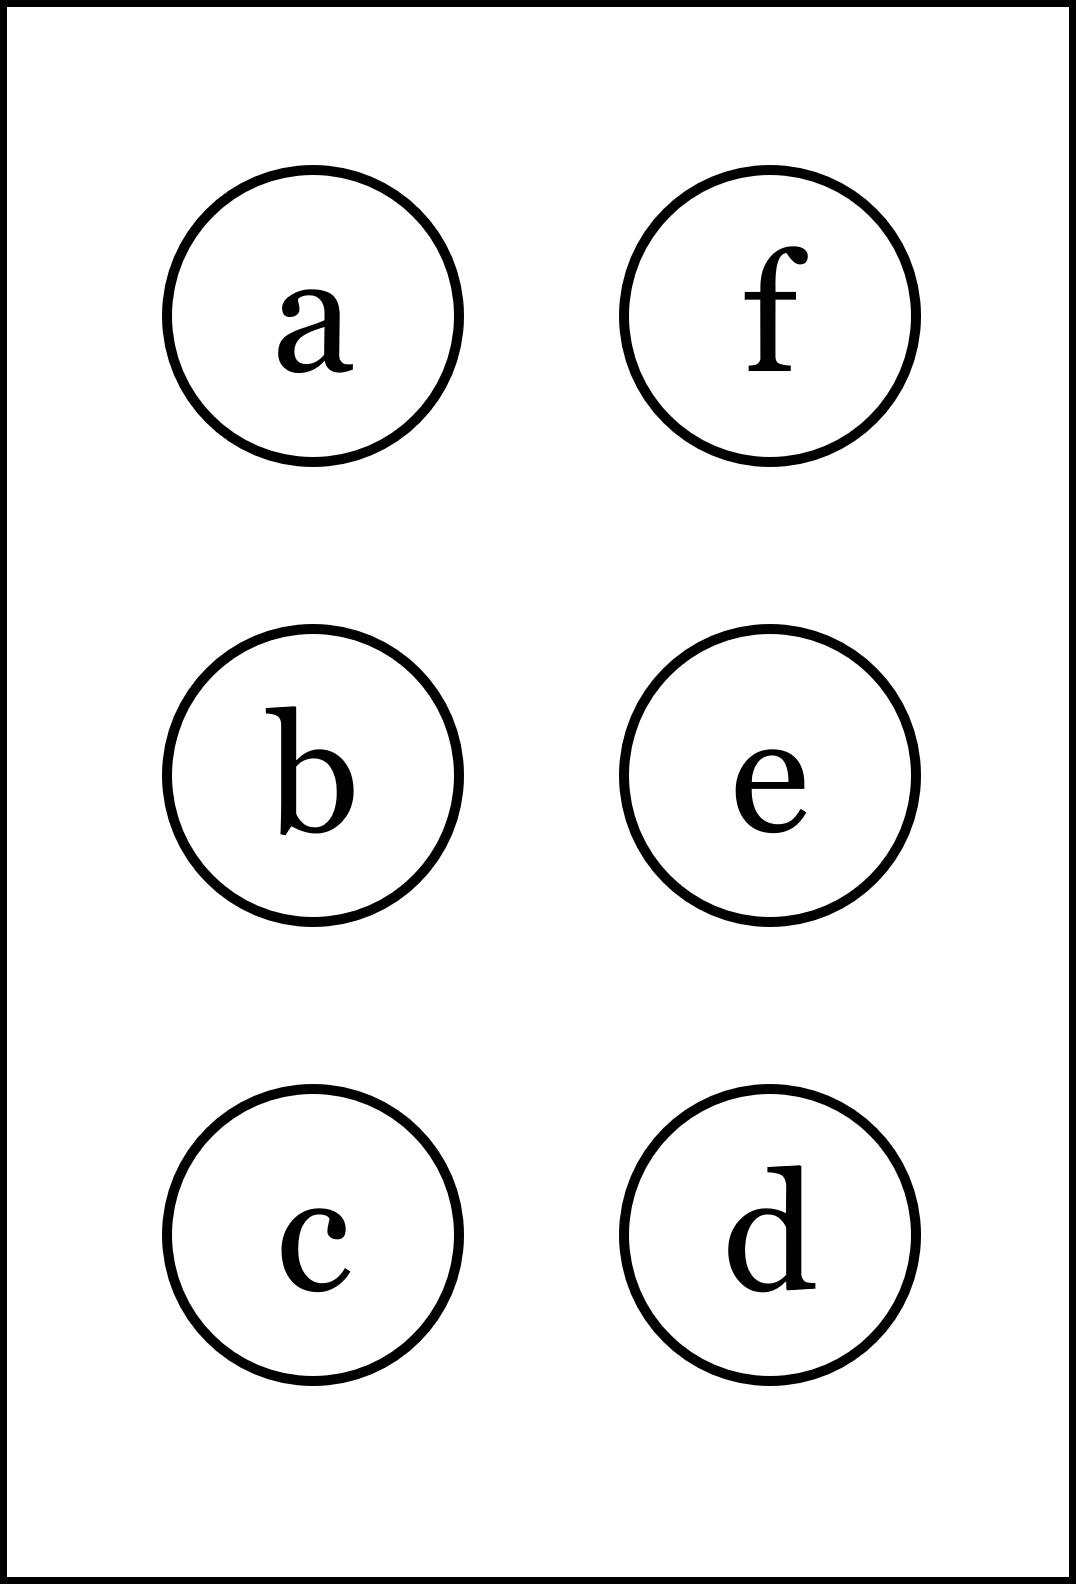
\includegraphics[height=40mm]{../images/braille.png}
{\small Písmeno Braillovej abecedy}
\end{center}
\end{minipage}
\end{center}
\end{minipage}
&
\begin{minipage}[c][104.5mm][t]{0.5\linewidth}
\begin{center}
\vspace{7mm}
{\huge Derivácie, skupina \textit{Delta $\delta$} -\romannumeral2}\\[5mm]
\textit{Meno:}\phantom{xxxxxxxxxxxxxxxxxxxxxxxxxxxxxxxxxxxxxxxxxxxxxxxxxxxxxxxxxxxxxxxxx}\\[5mm]
\begin{minipage}{0.95\linewidth}
\begin{center}
\textbf{Vypočítej derivace.} Pokud se výsledky shodují s těmi za otazníky,\\tak napravo obarvi příslušející kroužek načerno. \textbf{Spolu odevzdejte výsledné slovo}.
\end{center}
\end{minipage}
\\[1mm]
\begin{minipage}{0.79\linewidth}
\begin{center}
\begin{varwidth}{\linewidth}
\begin{enumerate}
\normalsize
\item $-3x^4+x^3+8x^2+2x-1$\quad \dotfill\; ???\;\dotfill \quad $-12x^3+3x^2+16x+2$
\item $\cfrac{4x^2+x-5}{-5x-5}$\quad \dotfill\; ???\;\dotfill \quad $\cfrac{-20x^2+40x-30}{25x^2+50x+25}$
\item $\frac{3}{x}\sqrt{2x-6}$\quad \dotfill\; ???\;\dotfill \quad $\frac{-6x+36}{x^2 \sqrt{\smash[b]{2x-6}}}$
\item $e^{4x^2-3x-3}$\quad \dotfill\; ???\;\dotfill \quad $e^{4x^2-3x-3}$
\item $\ln{\left(\frac{-8x+8}{-x+2}\right)}$\quad \dotfill\; ???\;\dotfill \quad $\frac{-8}{-8x+8}-\frac{-1}{-x+2}$
\item $\frac{e^{-5x+4}}{2x+4}$\quad \dotfill\; ???\;\dotfill \quad $\frac{+10x-22}{(2x+4)^2}e^{-5x+4}$
\end{enumerate}
\end{varwidth}
\end{center}
\end{minipage}
\begin{minipage}{0.20\linewidth}
\begin{center}
{\Huge\bfseries 2.} \\[2mm]
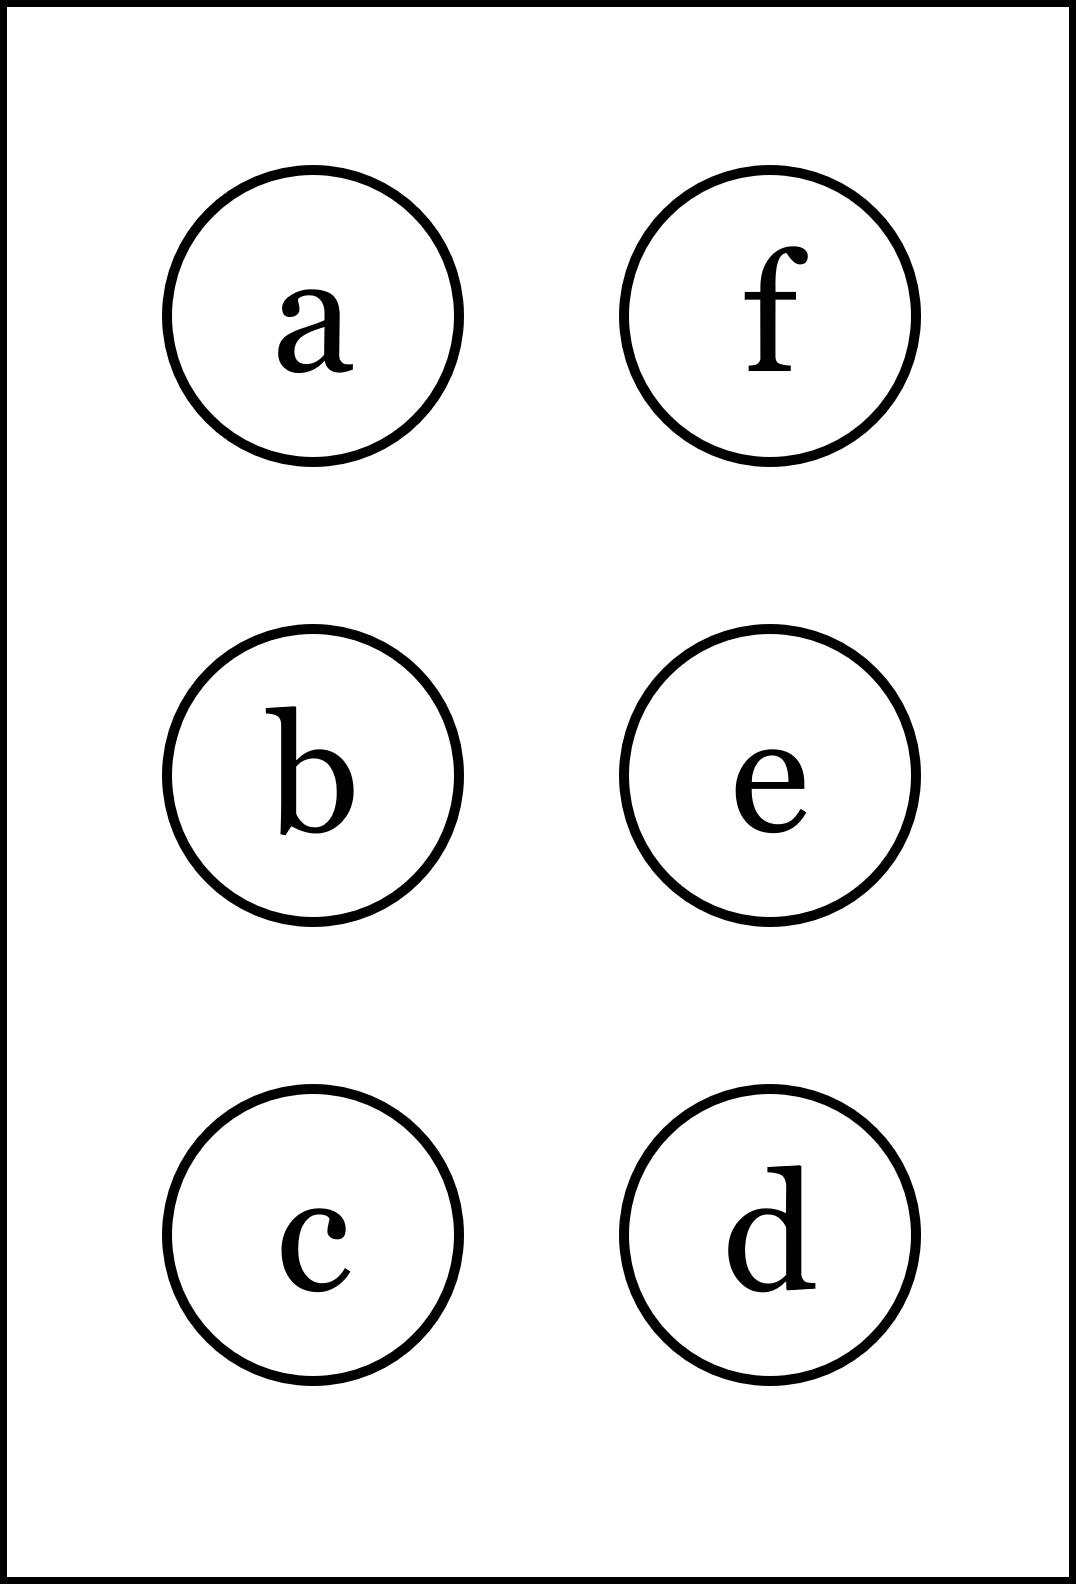
\includegraphics[height=40mm]{../images/braille.png}
{\small Písmeno Braillovej abecedy}
\end{center}
\end{minipage}
\end{center}
\end{minipage}
\\ \hdashline
\begin{minipage}[c][104.5mm][t]{0.5\linewidth}
\begin{center}
\vspace{7mm}
{\huge Derivácie, skupina \textit{Delta $\delta$} -\romannumeral3}\\[5mm]
\textit{Meno:}\phantom{xxxxxxxxxxxxxxxxxxxxxxxxxxxxxxxxxxxxxxxxxxxxxxxxxxxxxxxxxxxxxxxxx}\\[5mm]
\begin{minipage}{0.95\linewidth}
\begin{center}
\textbf{Vypočítej derivace.} Pokud se výsledky shodují s těmi za otazníky,\\tak napravo obarvi příslušející kroužek načerno. \textbf{Spolu odevzdejte výsledné slovo}.
\end{center}
\end{minipage}
\\[1mm]
\begin{minipage}{0.79\linewidth}
\begin{center}
\begin{varwidth}{\linewidth}
\begin{enumerate}
\normalsize
\item $-8x^4+7x^3+x^2+4x+3$\quad \dotfill\; ???\;\dotfill \quad $-32x^3+21x^2+2x+4$
\item $\cfrac{-3x^2-2x+3}{x+4}$\quad \dotfill\; ???\;\dotfill \quad $\cfrac{-3x^2-24x-11}{x^2+8x+16}$
\item $\frac{7}{x}\sqrt{-2x-4}$\quad \dotfill\; ???\;\dotfill \quad $\frac{14x+56}{2x^2 \sqrt{\smash[b]{-2x-4}}}$
\item $e^{2x^2-7x-2}$\quad \dotfill\; ???\;\dotfill \quad $e^{2x^2-7x-2}$
\item $\ln{\left(\frac{x+1}{-2x-1}\right)}$\quad \dotfill\; ???\;\dotfill \quad $\frac{1}{x+1}+\frac{-2}{-2x-1}$
\item $\frac{e^{-5x-2}}{x-3}$\quad \dotfill\; ???\;\dotfill \quad $\frac{-5x+14}{(x-3)^2}e^{-5x-2}$
\end{enumerate}
\end{varwidth}
\end{center}
\end{minipage}
\begin{minipage}{0.20\linewidth}
\begin{center}
{\Huge\bfseries 3.} \\[2mm]
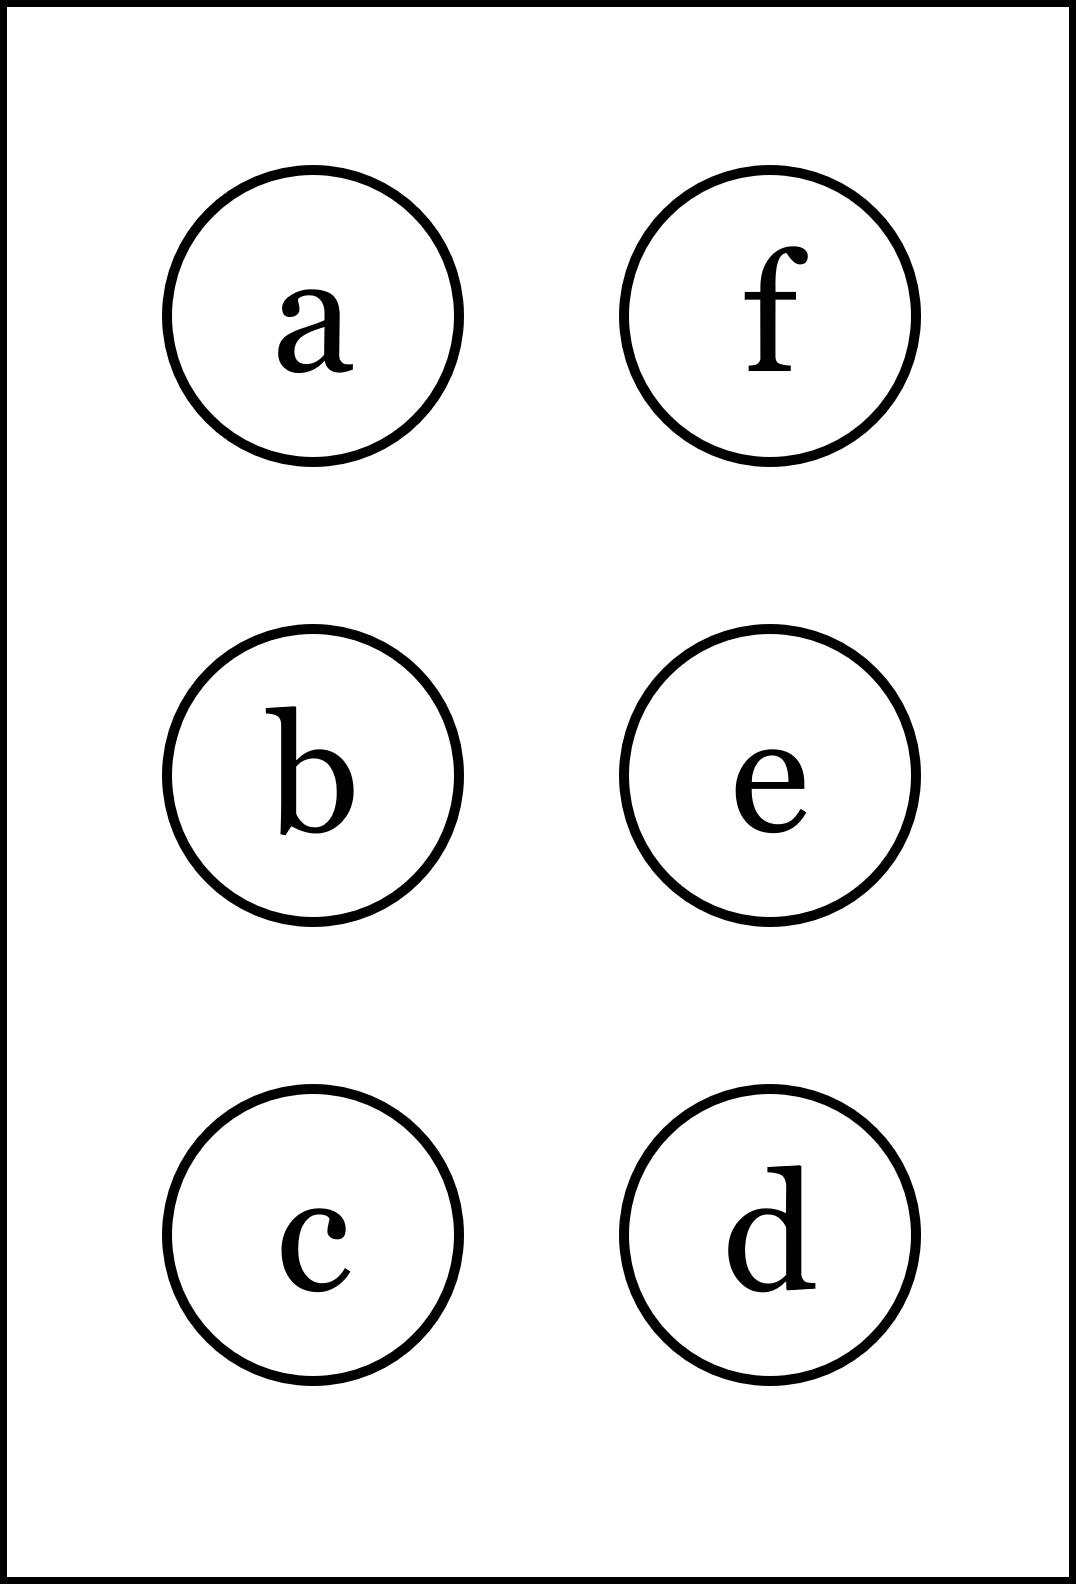
\includegraphics[height=40mm]{../images/braille.png}
{\small Písmeno Braillovej abecedy}
\end{center}
\end{minipage}
\end{center}
\end{minipage}
&
\begin{minipage}[c][104.5mm][t]{0.5\linewidth}
\begin{center}
\vspace{7mm}
{\huge Derivácie, skupina \textit{Delta $\delta$} -\romannumeral4}\\[5mm]
\textit{Meno:}\phantom{xxxxxxxxxxxxxxxxxxxxxxxxxxxxxxxxxxxxxxxxxxxxxxxxxxxxxxxxxxxxxxxxx}\\[5mm]
\begin{minipage}{0.95\linewidth}
\begin{center}
\textbf{Vypočítej derivace.} Pokud se výsledky shodují s těmi za otazníky,\\tak napravo obarvi příslušející kroužek načerno. \textbf{Spolu odevzdejte výsledné slovo}.
\end{center}
\end{minipage}
\\[1mm]
\begin{minipage}{0.79\linewidth}
\begin{center}
\begin{varwidth}{\linewidth}
\begin{enumerate}
\normalsize
\item $-8x^4+5x^3+x^2+7x-7$\quad \dotfill\; ???\;\dotfill \quad $-32x^3+15x^2+2x+7$
\item $\cfrac{6x^2-3x-2}{-2x+4}$\quad \dotfill\; ???\;\dotfill \quad $\cfrac{-12x^2-48x-16}{4x^2-16x+16}$
\item $\frac{-3}{x}\sqrt{3x-7}$\quad \dotfill\; ???\;\dotfill \quad $\frac{9x-42}{x^2 \sqrt{\smash[b]{3x-7}}}$
\item $e^{-x^2+x-7}$\quad \dotfill\; ???\;\dotfill \quad $e^{-x^2+x-7}$
\item $\ln{\left(\frac{x-5}{8x+7}\right)}$\quad \dotfill\; ???\;\dotfill \quad $\frac{1}{x-5}+\frac{8}{8x+7}$
\item $\frac{e^{-x+6}}{-2x-2}$\quad \dotfill\; ???\;\dotfill \quad $\frac{-2x+4}{(-2x-2)^2}e^{-x+6}$
\end{enumerate}
\end{varwidth}
\end{center}
\end{minipage}
\begin{minipage}{0.20\linewidth}
\begin{center}
{\Huge\bfseries 4.} \\[2mm]
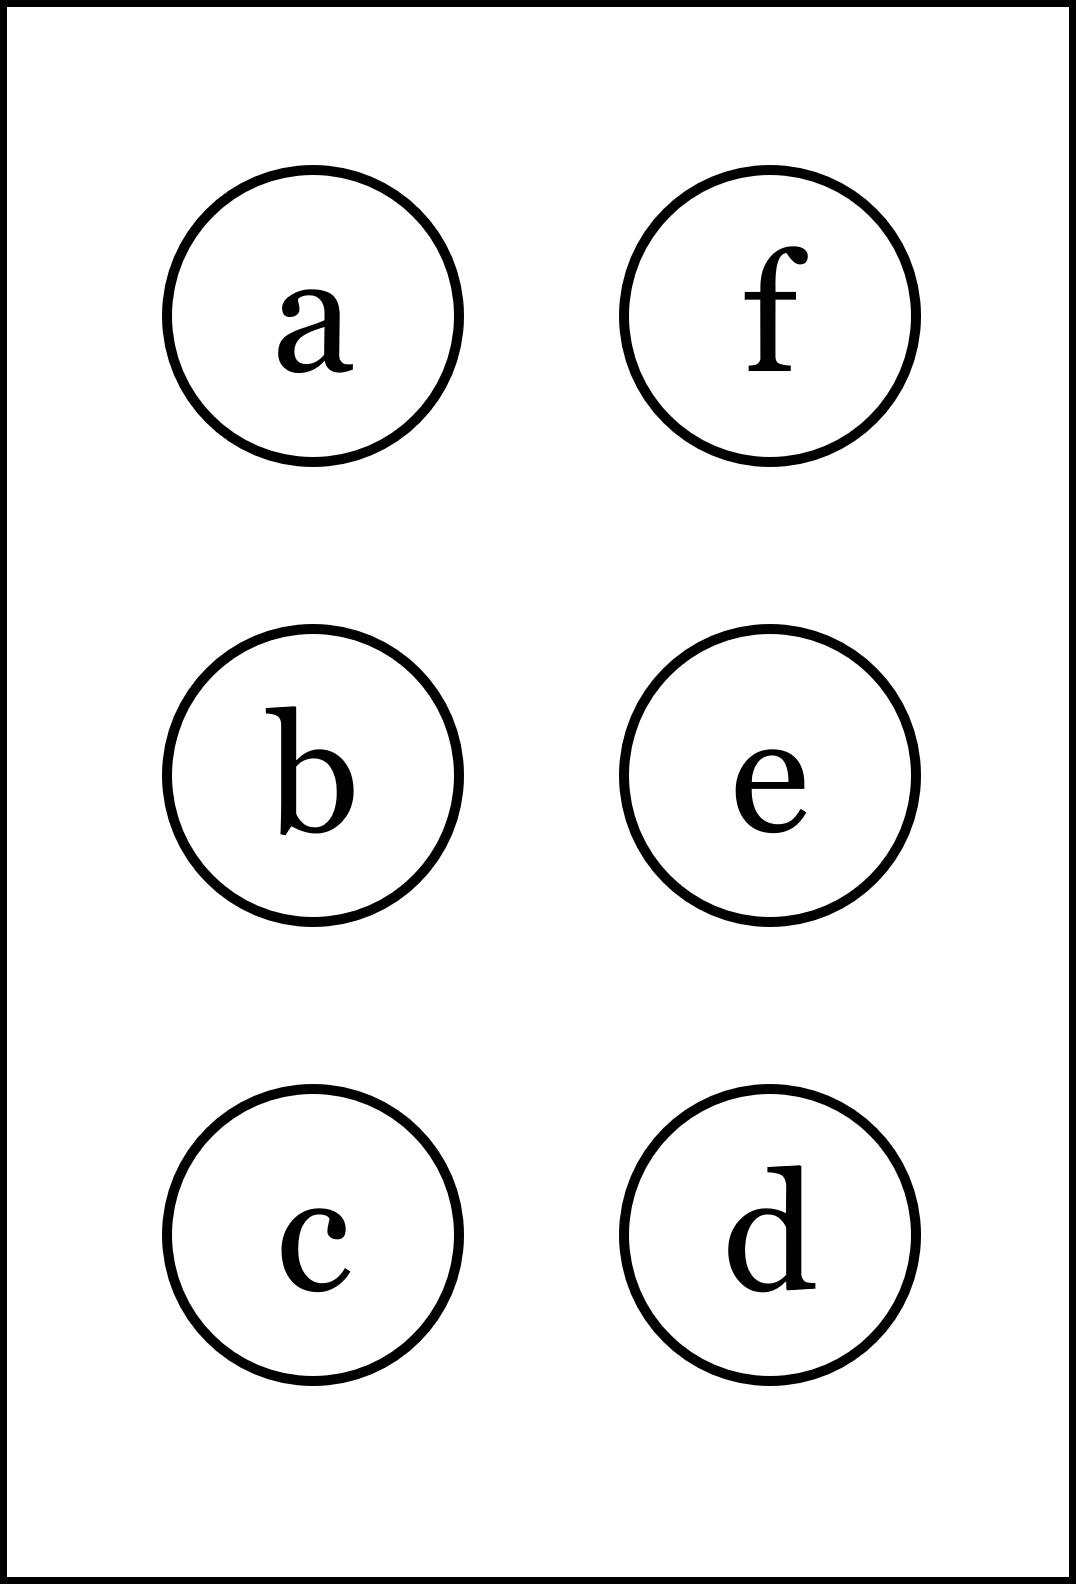
\includegraphics[height=40mm]{../images/braille.png}
{\small Písmeno Braillovej abecedy}
\end{center}
\end{minipage}
\end{center}
\end{minipage}
%
\end{tabular}
\newpage
\thispagestyle{empty}
\begin{tabular}{c:c}
\begin{minipage}[c][104.5mm][t]{0.5\linewidth}
\begin{center}
\vspace{7mm}
{\huge Derivácie, skupina \textit{Epsilon $\epsilon$} -\romannumeral1}\\[5mm]
\textit{Meno:}\phantom{xxxxxxxxxxxxxxxxxxxxxxxxxxxxxxxxxxxxxxxxxxxxxxxxxxxxxxxxxxxxxxxxx}\\[5mm]
\begin{minipage}{0.95\linewidth}
\begin{center}
\textbf{Vypočítej derivace.} Pokud se výsledky shodují s těmi za otazníky,\\tak napravo obarvi příslušející kroužek načerno. \textbf{Spolu odevzdejte výsledné slovo}.
\end{center}
\end{minipage}
\\[1mm]
\begin{minipage}{0.79\linewidth}
\begin{center}
\begin{varwidth}{\linewidth}
\begin{enumerate}
\normalsize
\item $4x^4+7x^3+6x^2-2x+7$\quad \dotfill\; ???\;\dotfill \quad $16x^3+21x^2+12x-2$
\item $\cfrac{3x^2-2x-2}{5x+1}$\quad \dotfill\; ???\;\dotfill \quad $\cfrac{15x^2+6x+8}{25x^2+10x+1}$
\item $\frac{4}{x}\sqrt{-x+4}$\quad \dotfill\; ???\;\dotfill \quad $\frac{4x-32}{x^2 \sqrt{\smash[b]{-x+4}}}$
\item $e^{-2x^2+6x+2}$\quad \dotfill\; ???\;\dotfill \quad $e^{-2x^2+6x+2}$
\item $\ln{\left(\frac{-3x+1}{x+2}\right)}$\quad \dotfill\; ???\;\dotfill \quad $\frac{-3}{-3x+1}-\frac{1}{x+2}$
\item $\frac{e^{-6x-9}}{-9x+6}$\quad \dotfill\; ???\;\dotfill \quad $\frac{-54x-27}{(-9x+6)^2}e^{-6x-9}$
\end{enumerate}
\end{varwidth}
\end{center}
\end{minipage}
\begin{minipage}{0.20\linewidth}
\begin{center}
{\Huge\bfseries 1.} \\[2mm]
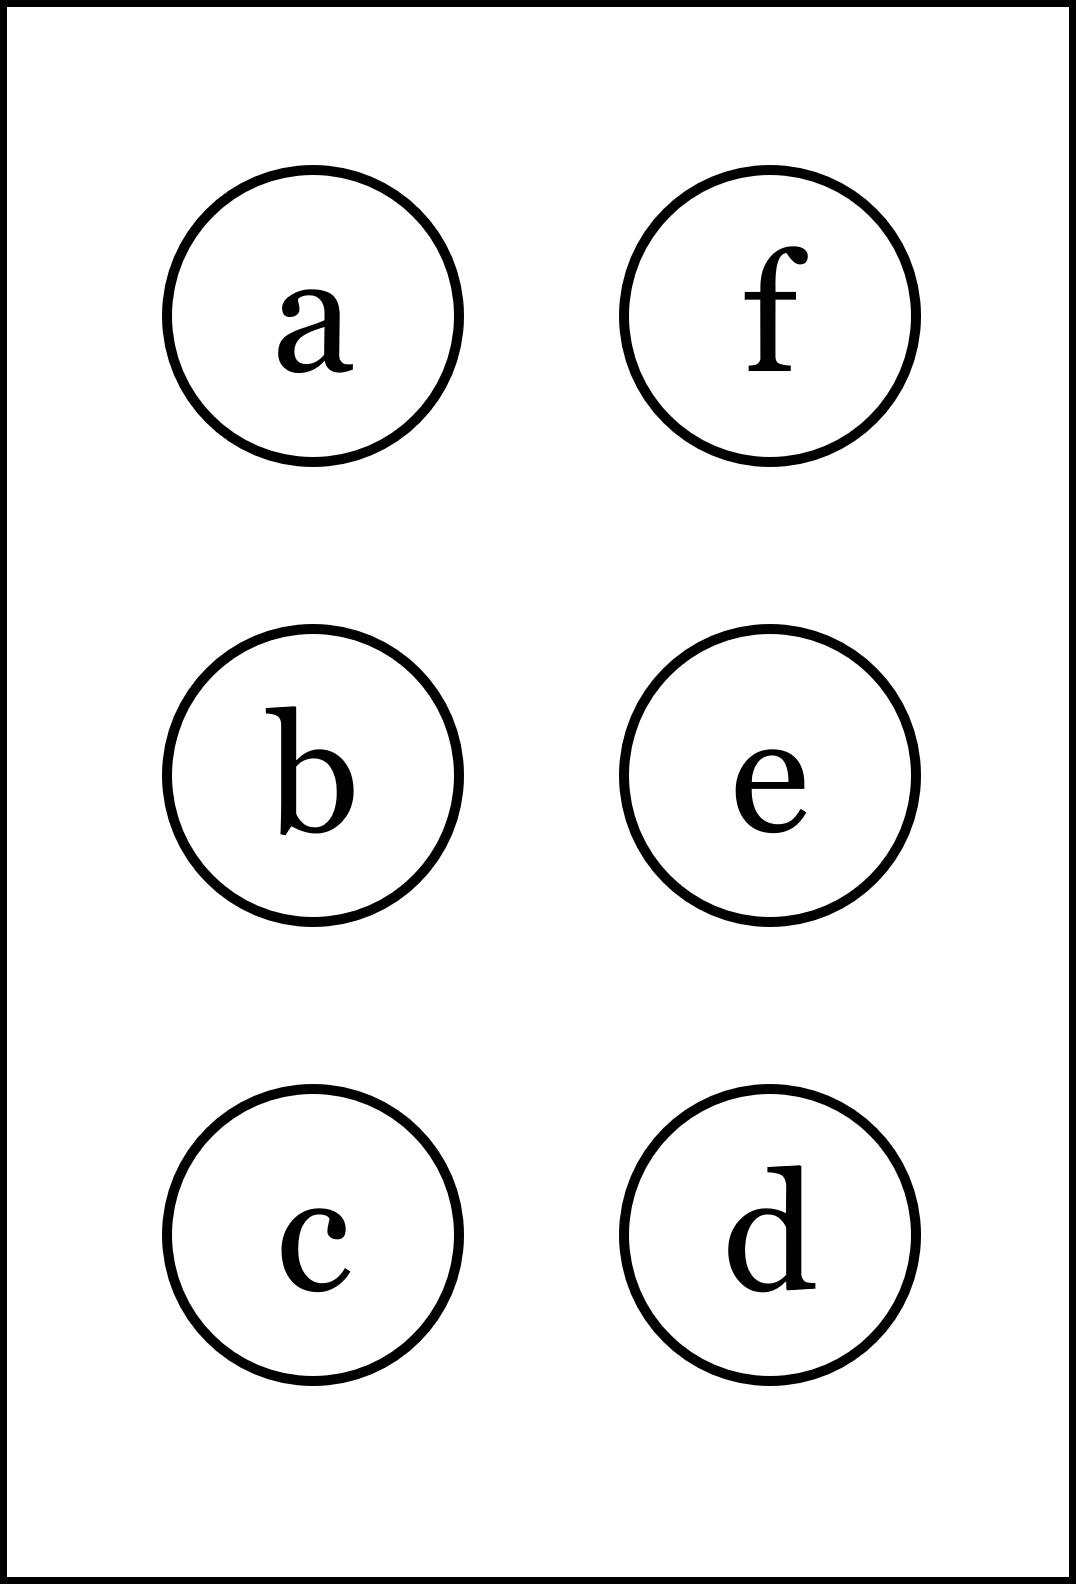
\includegraphics[height=40mm]{../images/braille.png}
{\small Písmeno Braillovej abecedy}
\end{center}
\end{minipage}
\end{center}
\end{minipage}
&
\begin{minipage}[c][104.5mm][t]{0.5\linewidth}
\begin{center}
\vspace{7mm}
{\huge Derivácie, skupina \textit{Epsilon $\epsilon$} -\romannumeral2}\\[5mm]
\textit{Meno:}\phantom{xxxxxxxxxxxxxxxxxxxxxxxxxxxxxxxxxxxxxxxxxxxxxxxxxxxxxxxxxxxxxxxxx}\\[5mm]
\begin{minipage}{0.95\linewidth}
\begin{center}
\textbf{Vypočítej derivace.} Pokud se výsledky shodují s těmi za otazníky,\\tak napravo obarvi příslušející kroužek načerno. \textbf{Spolu odevzdejte výsledné slovo}.
\end{center}
\end{minipage}
\\[1mm]
\begin{minipage}{0.79\linewidth}
\begin{center}
\begin{varwidth}{\linewidth}
\begin{enumerate}
\normalsize
\item $4x^4-2x^3+x^2+x+3$\quad \dotfill\; ???\;\dotfill \quad $16x^3-6x^2+2x+1$
\item $\cfrac{-3x^2+4x-6}{-3x+5}$\quad \dotfill\; ???\;\dotfill \quad $\cfrac{9x^2+30x+2}{9x^2-30x+25}$
\item $\frac{-2}{x}\sqrt{-3x-5}$\quad \dotfill\; ???\;\dotfill \quad $\frac{-6x-20}{x^2 \sqrt{\smash[b]{-3x-5}}}$
\item $e^{-8x^2+x+2}$\quad \dotfill\; ???\;\dotfill \quad $e^{-8x^2+x+2}$
\item $\ln{\left(\frac{-2x+4}{-3x+8}\right)}$\quad \dotfill\; ???\;\dotfill \quad $\frac{-2}{-2x+4}+\frac{-3}{-3x+8}$
\item $\frac{e^{-8x+4}}{-5x-3}$\quad \dotfill\; ???\;\dotfill \quad $\frac{-40x+29}{(-5x-3)^2}e^{-8x+4}$
\end{enumerate}
\end{varwidth}
\end{center}
\end{minipage}
\begin{minipage}{0.20\linewidth}
\begin{center}
{\Huge\bfseries 2.} \\[2mm]
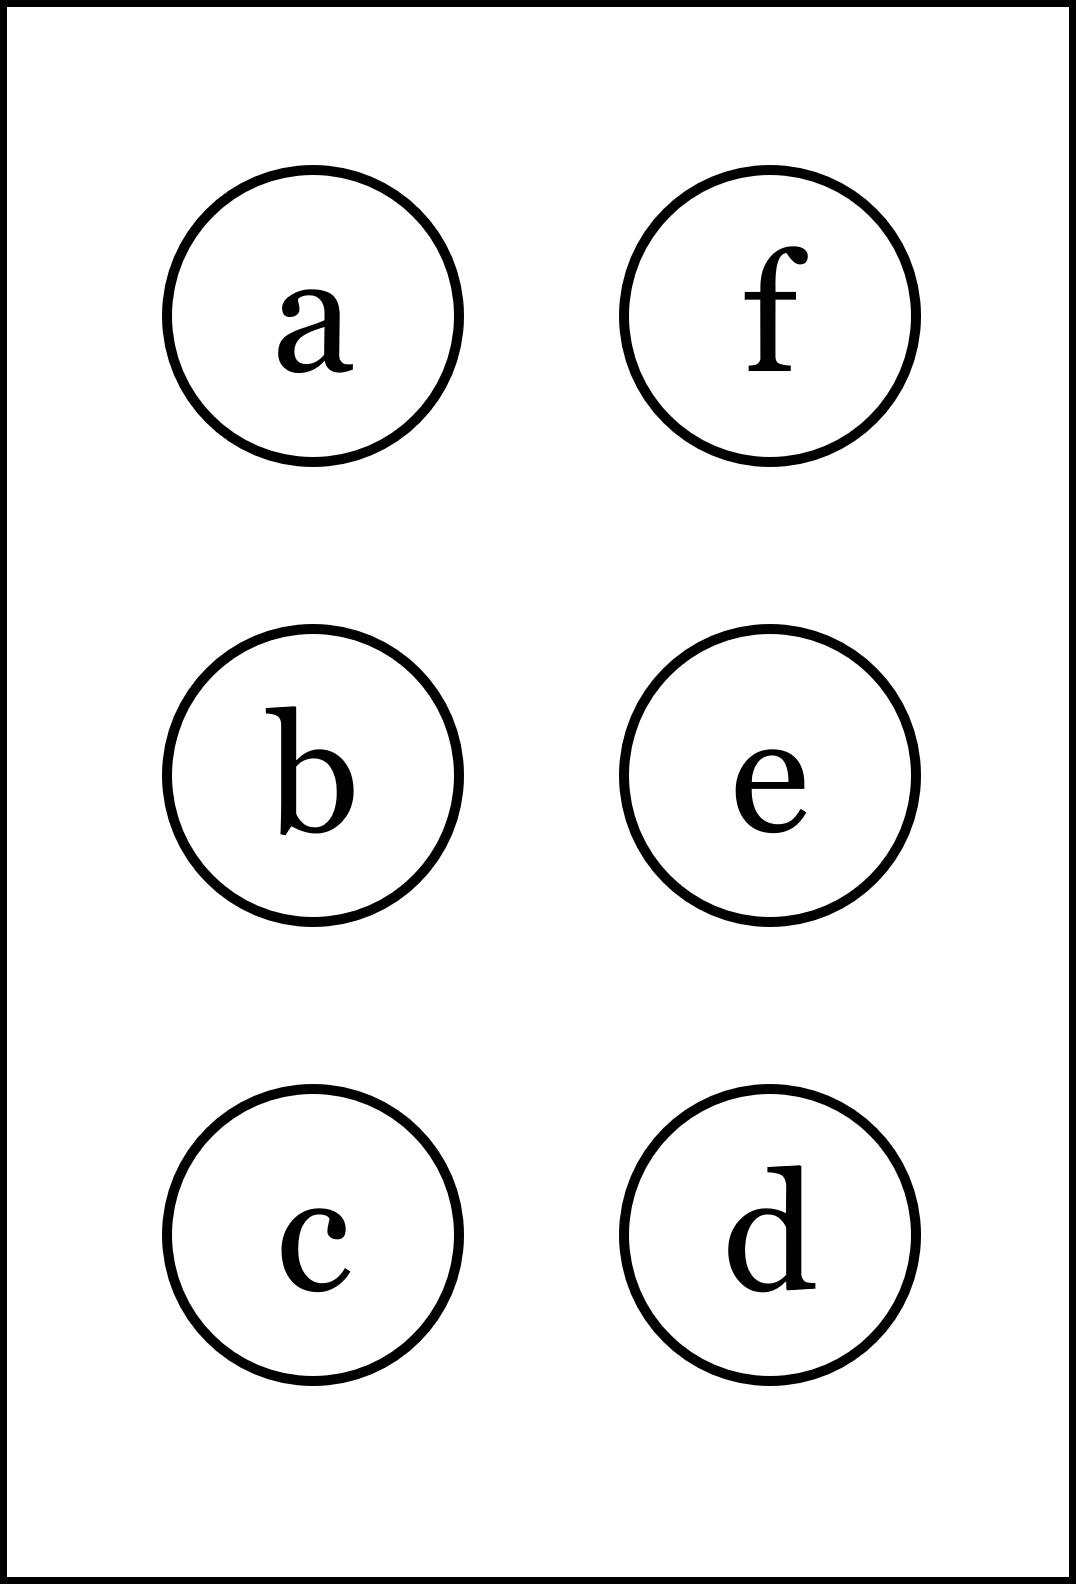
\includegraphics[height=40mm]{../images/braille.png}
{\small Písmeno Braillovej abecedy}
\end{center}
\end{minipage}
\end{center}
\end{minipage}
\\ \hdashline
\begin{minipage}[c][104.5mm][t]{0.5\linewidth}
\begin{center}
\vspace{7mm}
{\huge Derivácie, skupina \textit{Epsilon $\epsilon$} -\romannumeral3}\\[5mm]
\textit{Meno:}\phantom{xxxxxxxxxxxxxxxxxxxxxxxxxxxxxxxxxxxxxxxxxxxxxxxxxxxxxxxxxxxxxxxxx}\\[5mm]
\begin{minipage}{0.95\linewidth}
\begin{center}
\textbf{Vypočítej derivace.} Pokud se výsledky shodují s těmi za otazníky,\\tak napravo obarvi příslušející kroužek načerno. \textbf{Spolu odevzdejte výsledné slovo}.
\end{center}
\end{minipage}
\\[1mm]
\begin{minipage}{0.79\linewidth}
\begin{center}
\begin{varwidth}{\linewidth}
\begin{enumerate}
\normalsize
\item $-7x^4+5x^3-2x^2-2x+6$\quad \dotfill\; ???\;\dotfill \quad $-28x^3+15x^2-4x-2$
\item $\cfrac{-6x^2-4x+2}{3x+6}$\quad \dotfill\; ???\;\dotfill \quad $\cfrac{-18x^2+72x-30}{9x^2+36x+36}$
\item $\frac{9}{x}\sqrt{2x+2}$\quad \dotfill\; ???\;\dotfill \quad $\frac{-18x-36}{2x^2 \sqrt{\smash[b]{2x+2}}}$
\item $e^{5x^2-7x+1}$\quad \dotfill\; ???\;\dotfill \quad $e^{5x^2-7x+1}$
\item $\ln{\left(\frac{-7x+3}{-3x-3}\right)}$\quad \dotfill\; ???\;\dotfill \quad $\frac{-7}{-7x+3}-\frac{-3}{-3x-3}$
\item $\frac{e^{6x-4}}{-3x+8}$\quad \dotfill\; ???\;\dotfill \quad $\frac{-18x+51}{(-3x+8)^2}e^{6x-4}$
\end{enumerate}
\end{varwidth}
\end{center}
\end{minipage}
\begin{minipage}{0.20\linewidth}
\begin{center}
{\Huge\bfseries 3.} \\[2mm]
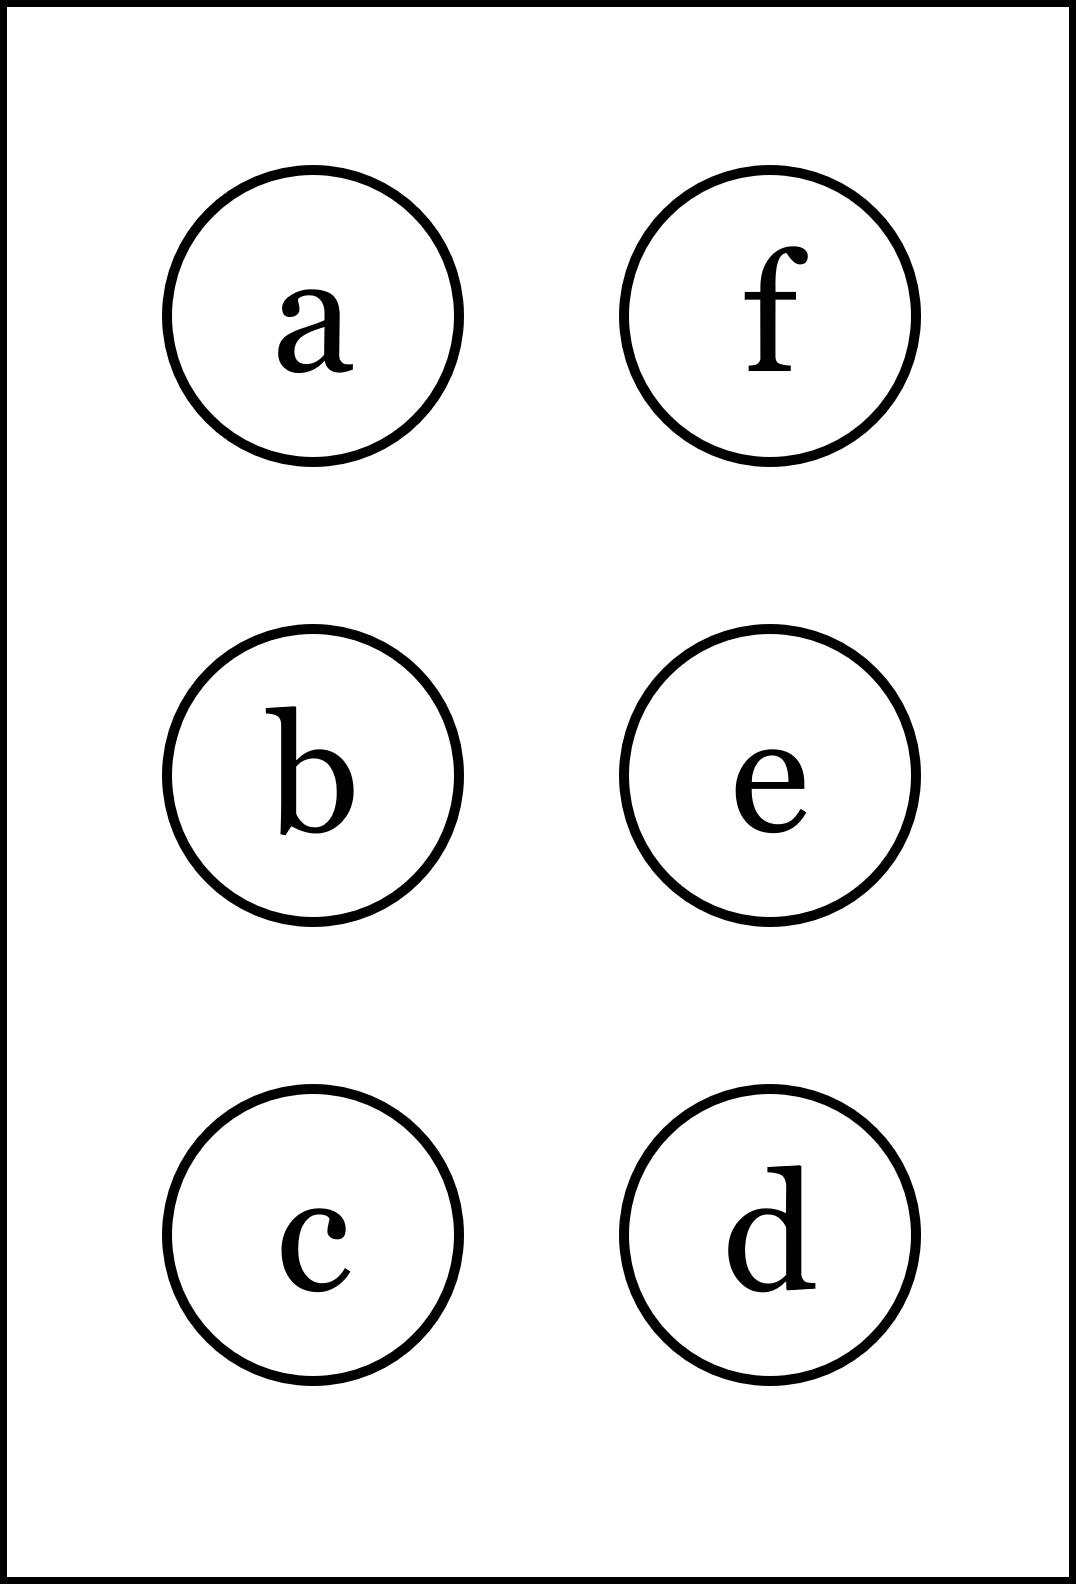
\includegraphics[height=40mm]{../images/braille.png}
{\small Písmeno Braillovej abecedy}
\end{center}
\end{minipage}
\end{center}
\end{minipage}
&
\begin{minipage}[c][104.5mm][t]{0.5\linewidth}
\begin{center}
\vspace{7mm}
{\huge Derivácie, skupina \textit{Epsilon $\epsilon$} -\romannumeral4}\\[5mm]
\textit{Meno:}\phantom{xxxxxxxxxxxxxxxxxxxxxxxxxxxxxxxxxxxxxxxxxxxxxxxxxxxxxxxxxxxxxxxxx}\\[5mm]
\begin{minipage}{0.95\linewidth}
\begin{center}
\textbf{Vypočítej derivace.} Pokud se výsledky shodují s těmi za otazníky,\\tak napravo obarvi příslušející kroužek načerno. \textbf{Spolu odevzdejte výsledné slovo}.
\end{center}
\end{minipage}
\\[1mm]
\begin{minipage}{0.79\linewidth}
\begin{center}
\begin{varwidth}{\linewidth}
\begin{enumerate}
\normalsize
\item $3x^4-x^3-6x^2-x+2$\quad \dotfill\; ???\;\dotfill \quad $12x^3-3x^2-12x-1$
\item $\cfrac{x^2+4x-2}{-3x+3}$\quad \dotfill\; ???\;\dotfill \quad $\cfrac{-3x^2-6x+6}{9x^2-18x+9}$
\item $\frac{-5}{x}\sqrt{-3x-8}$\quad \dotfill\; ???\;\dotfill \quad $\frac{-15x-80}{x^2 \sqrt{\smash[b]{-3x-8}}}$
\item $e^{2x^2+5x+1}$\quad \dotfill\; ???\;\dotfill \quad $e^{2x^2+5x+1}$
\item $\ln{\left(\frac{-7x+1}{x+2}\right)}$\quad \dotfill\; ???\;\dotfill \quad $\frac{-7}{-7x+1}+\frac{1}{x+2}$
\item $\frac{e^{-3x-6}}{-2x+3}$\quad \dotfill\; ???\;\dotfill \quad $\frac{-6x-7}{(-2x+3)^2}e^{-3x-6}$
\end{enumerate}
\end{varwidth}
\end{center}
\end{minipage}
\begin{minipage}{0.20\linewidth}
\begin{center}
{\Huge\bfseries 4.} \\[2mm]
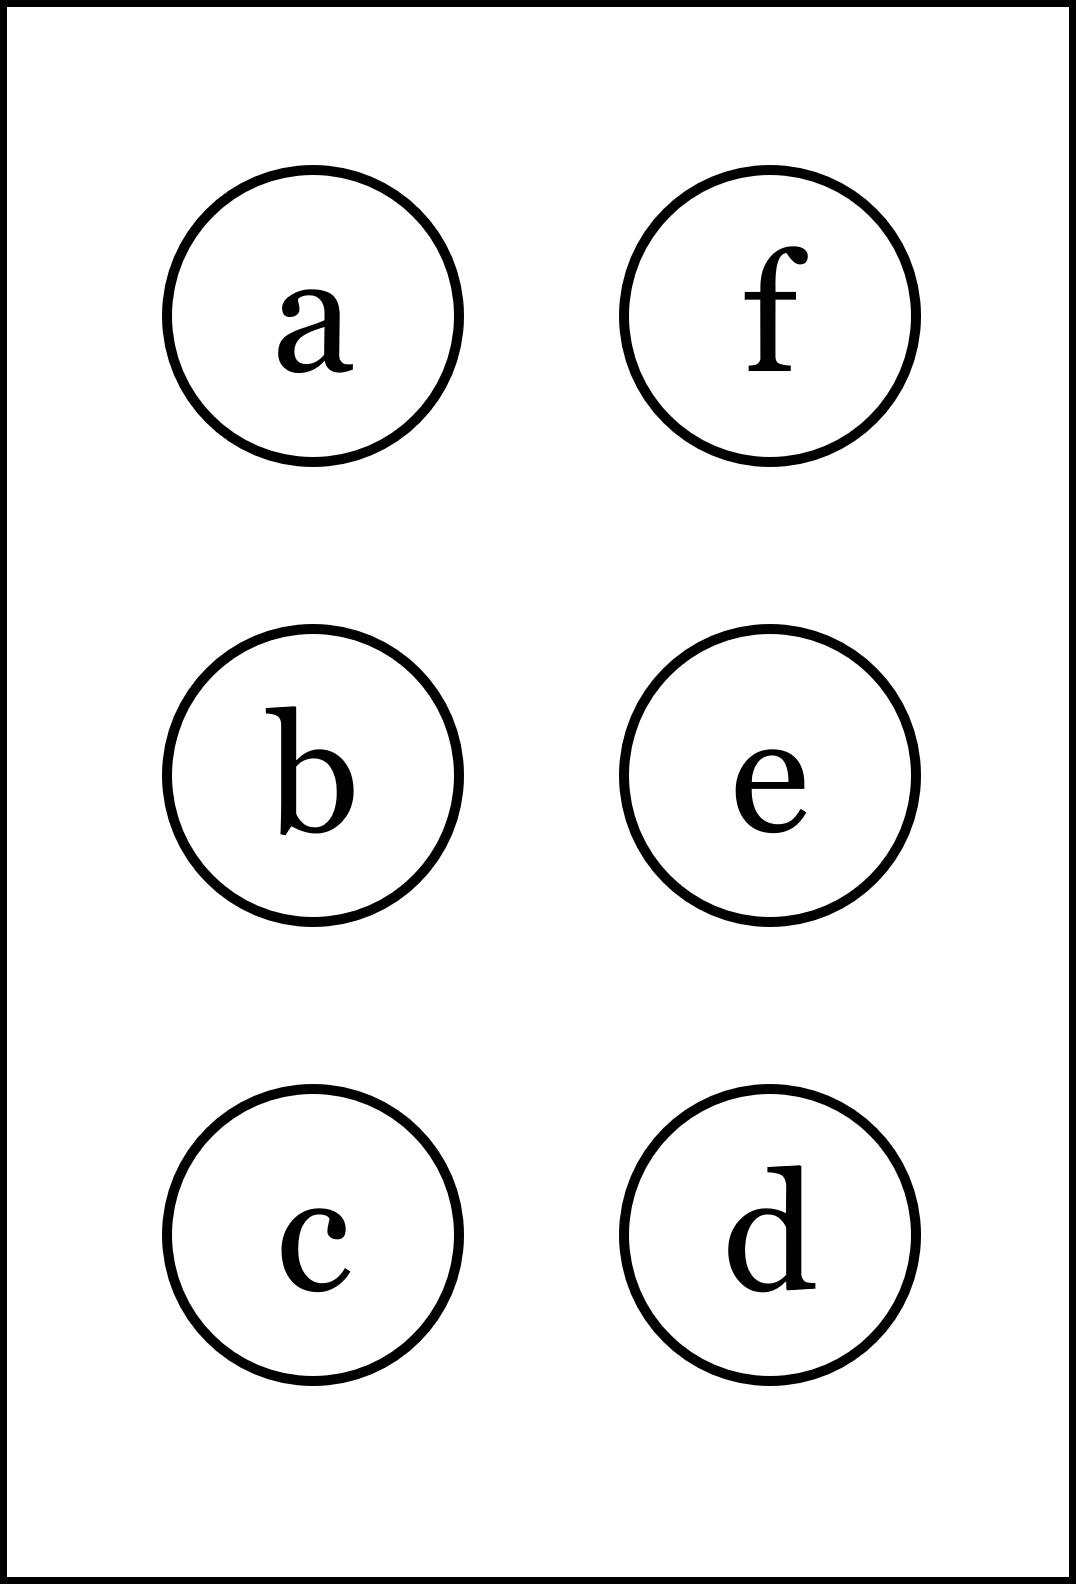
\includegraphics[height=40mm]{../images/braille.png}
{\small Písmeno Braillovej abecedy}
\end{center}
\end{minipage}
\end{center}
\end{minipage}
%
\end{tabular}
\newpage
\thispagestyle{empty}
\begin{tabular}{c:c}
\begin{minipage}[c][104.5mm][t]{0.5\linewidth}
\begin{center}
\vspace{7mm}
{\huge Derivácie, skupina \textit{Zeta $\zeta$} -\romannumeral1}\\[5mm]
\textit{Meno:}\phantom{xxxxxxxxxxxxxxxxxxxxxxxxxxxxxxxxxxxxxxxxxxxxxxxxxxxxxxxxxxxxxxxxx}\\[5mm]
\begin{minipage}{0.95\linewidth}
\begin{center}
\textbf{Vypočítej derivace.} Pokud se výsledky shodují s těmi za otazníky,\\tak napravo obarvi příslušející kroužek načerno. \textbf{Spolu odevzdejte výsledné slovo}.
\end{center}
\end{minipage}
\\[1mm]
\begin{minipage}{0.79\linewidth}
\begin{center}
\begin{varwidth}{\linewidth}
\begin{enumerate}
\normalsize
\item $-2x^4-3x^3-2x^2+9x+2$\quad \dotfill\; ???\;\dotfill \quad $-8x^3-9x^2-4x+9$
\item $\cfrac{-2x^2-x+1}{x+2}$\quad \dotfill\; ???\;\dotfill \quad $\cfrac{-2x^2+8x-3}{x^2+4x+4}$
\item $\frac{-5}{x}\sqrt{2x-4}$\quad \dotfill\; ???\;\dotfill \quad $\frac{10x-40}{2x^2 \sqrt{\smash[b]{2x-4}}}$
\item $e^{-8x^2+4x-9}$\quad \dotfill\; ???\;\dotfill \quad $e^{-8x^2+4x-9}$
\item $\ln{\left(\frac{-5x+7}{-5x+5}\right)}$\quad \dotfill\; ???\;\dotfill \quad $\frac{-5}{-5x+7}-\frac{-5}{-5x+5}$
\item $\frac{e^{2x-6}}{6x-1}$\quad \dotfill\; ???\;\dotfill \quad $\frac{-12x-8}{(6x-1)^2}e^{2x-6}$
\end{enumerate}
\end{varwidth}
\end{center}
\end{minipage}
\begin{minipage}{0.20\linewidth}
\begin{center}
{\Huge\bfseries 1.} \\[2mm]
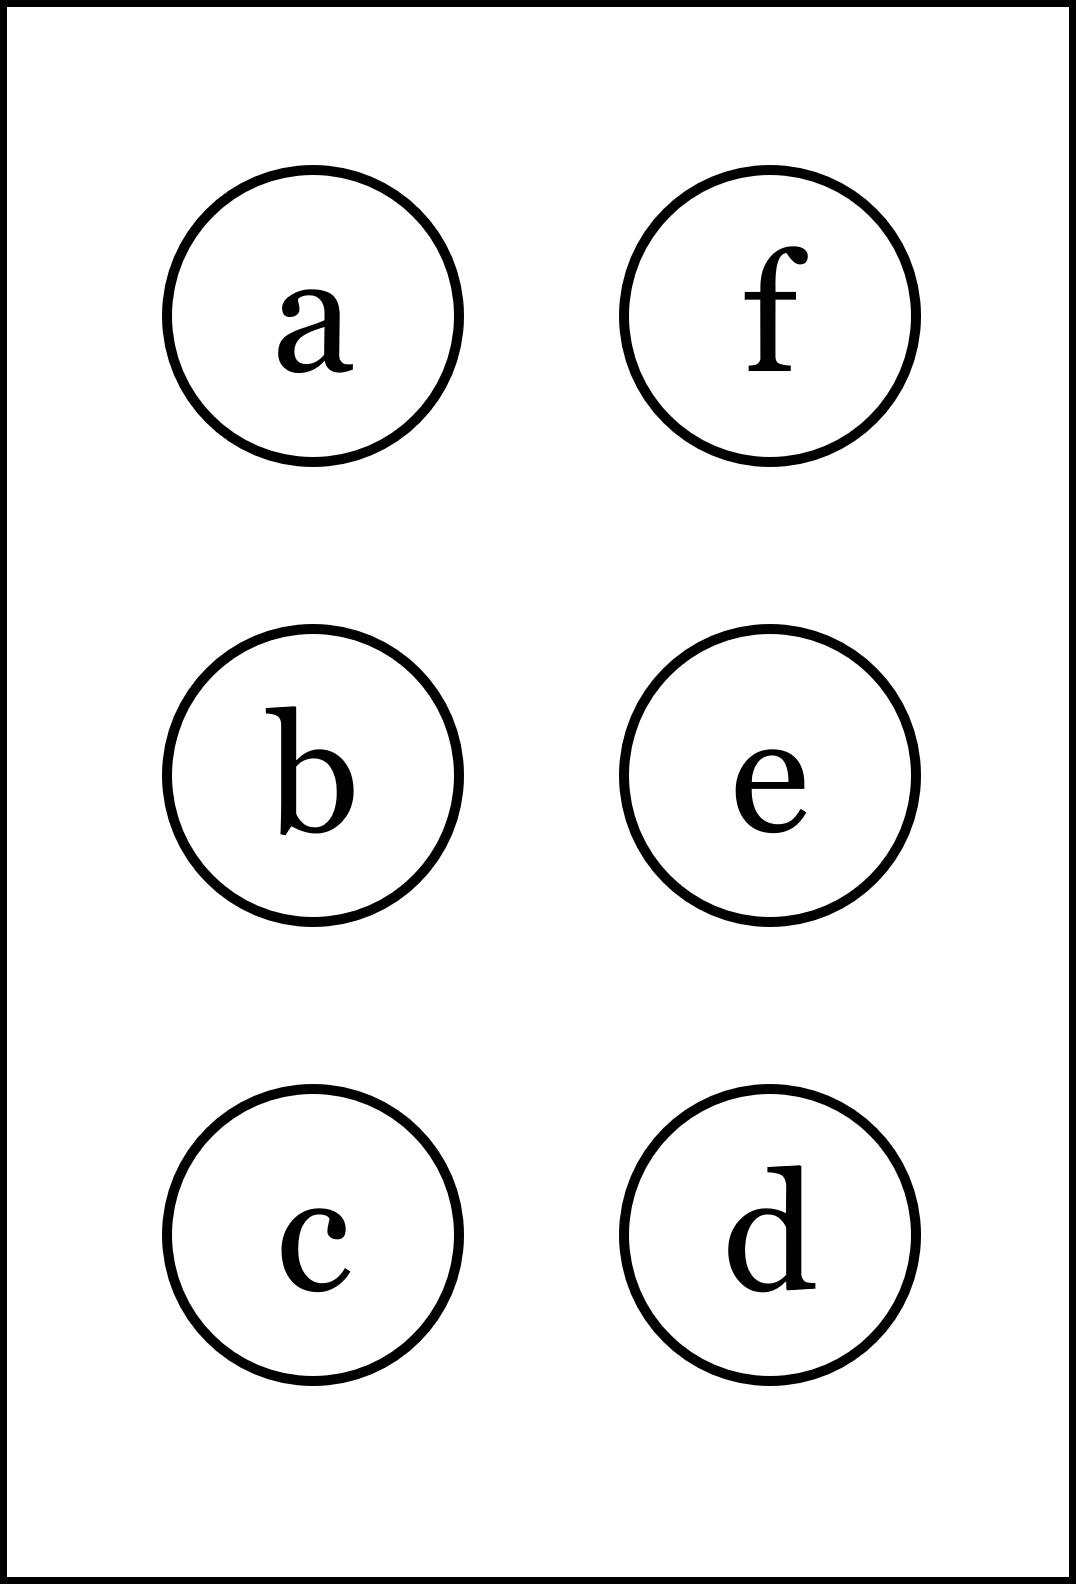
\includegraphics[height=40mm]{../images/braille.png}
{\small Písmeno Braillovej abecedy}
\end{center}
\end{minipage}
\end{center}
\end{minipage}
&
\begin{minipage}[c][104.5mm][t]{0.5\linewidth}
\begin{center}
\vspace{7mm}
{\huge Derivácie, skupina \textit{Zeta $\zeta$} -\romannumeral2}\\[5mm]
\textit{Meno:}\phantom{xxxxxxxxxxxxxxxxxxxxxxxxxxxxxxxxxxxxxxxxxxxxxxxxxxxxxxxxxxxxxxxxx}\\[5mm]
\begin{minipage}{0.95\linewidth}
\begin{center}
\textbf{Vypočítej derivace.} Pokud se výsledky shodují s těmi za otazníky,\\tak napravo obarvi příslušející kroužek načerno. \textbf{Spolu odevzdejte výsledné slovo}.
\end{center}
\end{minipage}
\\[1mm]
\begin{minipage}{0.79\linewidth}
\begin{center}
\begin{varwidth}{\linewidth}
\begin{enumerate}
\normalsize
\item $2x^4+7x^3-2x^2-2x+6$\quad \dotfill\; ???\;\dotfill \quad $8x^3+21x^2-4x-2$
\item $\cfrac{-x^2+2x-1}{-5x-2}$\quad \dotfill\; ???\;\dotfill \quad $\cfrac{5x^2+4x-9}{25x^2+20x+4}$
\item $\frac{-1}{x}\sqrt{4x+1}$\quad \dotfill\; ???\;\dotfill \quad $\frac{4x+2}{2x^2 \sqrt{\smash[b]{4x+1}}}$
\item $e^{9x^2-6x+4}$\quad \dotfill\; ???\;\dotfill \quad $e^{9x^2-6x+4}$
\item $\ln{\left(\frac{8x-3}{-7x-6}\right)}$\quad \dotfill\; ???\;\dotfill \quad $\frac{8}{8x-3}+\frac{-7}{-7x-6}$
\item $\frac{e^{2x+4}}{3x-5}$\quad \dotfill\; ???\;\dotfill \quad $\frac{-6x-13}{(3x-5)^2}e^{2x+4}$
\end{enumerate}
\end{varwidth}
\end{center}
\end{minipage}
\begin{minipage}{0.20\linewidth}
\begin{center}
{\Huge\bfseries 2.} \\[2mm]
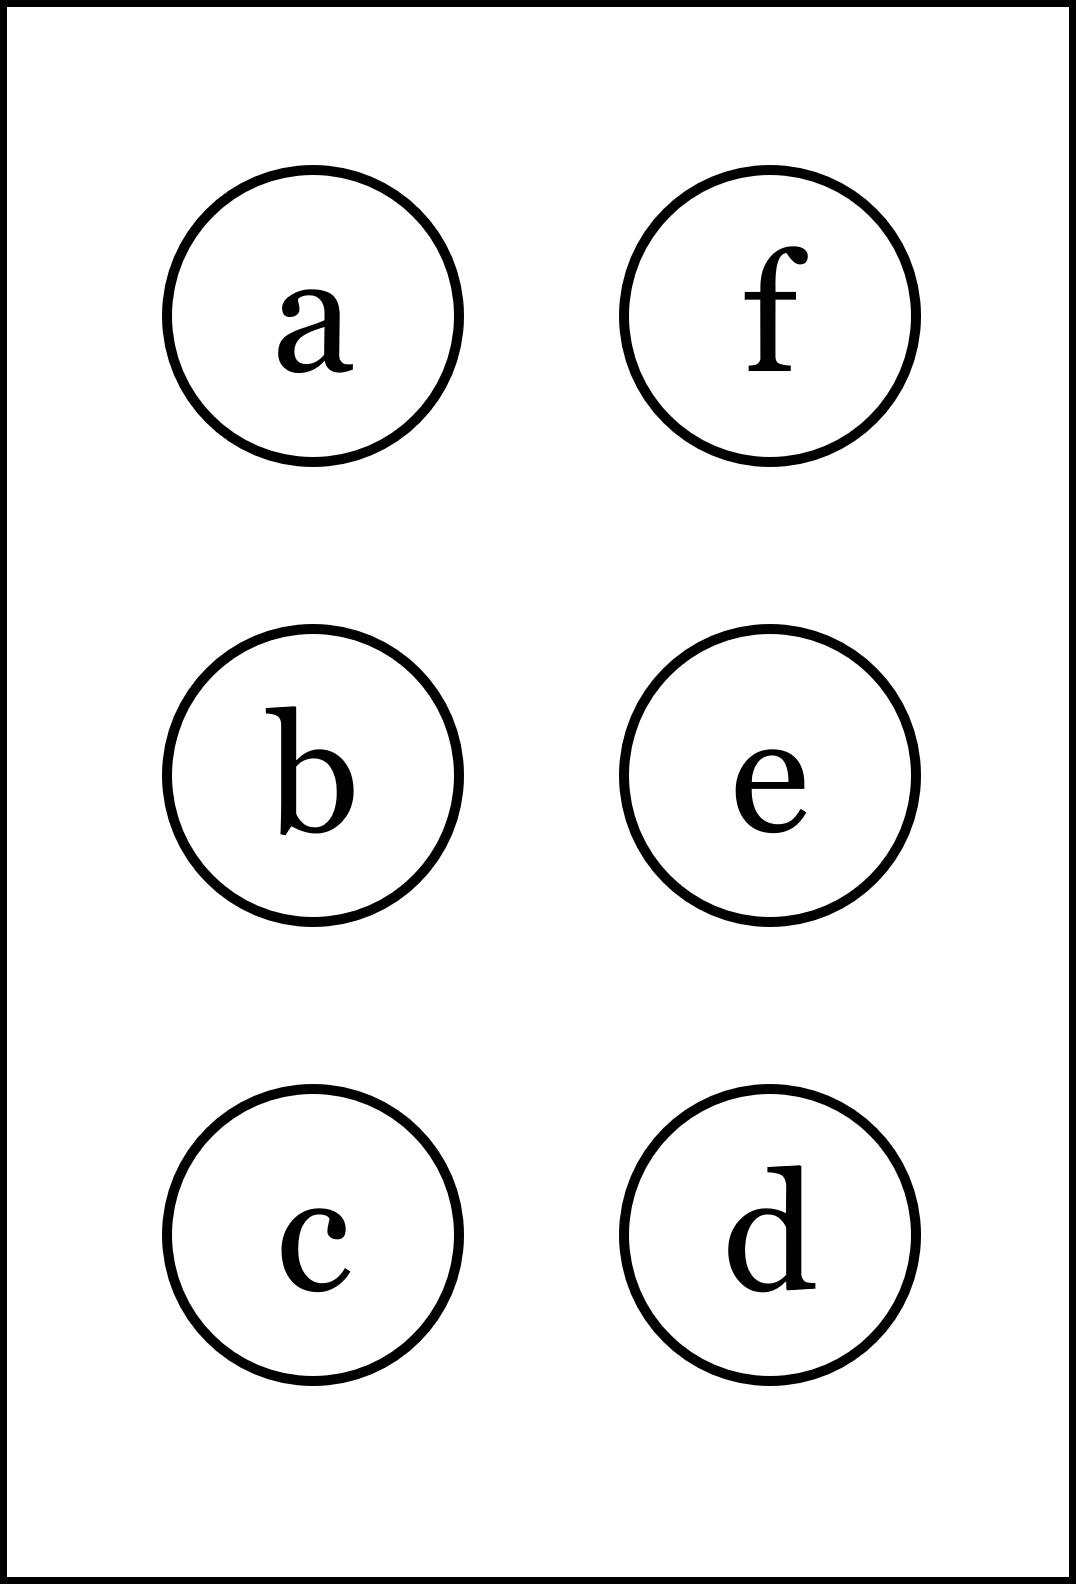
\includegraphics[height=40mm]{../images/braille.png}
{\small Písmeno Braillovej abecedy}
\end{center}
\end{minipage}
\end{center}
\end{minipage}
\\ \hdashline
\begin{minipage}[c][104.5mm][t]{0.5\linewidth}
\begin{center}
\vspace{7mm}
{\huge Derivácie, skupina \textit{Zeta $\zeta$} -\romannumeral3}\\[5mm]
\textit{Meno:}\phantom{xxxxxxxxxxxxxxxxxxxxxxxxxxxxxxxxxxxxxxxxxxxxxxxxxxxxxxxxxxxxxxxxx}\\[5mm]
\begin{minipage}{0.95\linewidth}
\begin{center}
\textbf{Vypočítej derivace.} Pokud se výsledky shodují s těmi za otazníky,\\tak napravo obarvi příslušející kroužek načerno. \textbf{Spolu odevzdejte výsledné slovo}.
\end{center}
\end{minipage}
\\[1mm]
\begin{minipage}{0.79\linewidth}
\begin{center}
\begin{varwidth}{\linewidth}
\begin{enumerate}
\normalsize
\item $3x^4-4x^3+8x^2-4x-6$\quad \dotfill\; ???\;\dotfill \quad $12x^3-12x^2+16x-4$
\item $\cfrac{-3x^2+5x-6}{-5x-6}$\quad \dotfill\; ???\;\dotfill \quad $\cfrac{15x^2-36x-60}{25x^2+60x+36}$
\item $\frac{-2}{x}\sqrt{9x+2}$\quad \dotfill\; ???\;\dotfill \quad $\frac{18x+8}{x^2 \sqrt{\smash[b]{9x+2}}}$
\item $e^{x^2-6x-5}$\quad \dotfill\; ???\;\dotfill \quad $e^{x^2-6x-5}$
\item $\ln{\left(\frac{x+4}{4x-3}\right)}$\quad \dotfill\; ???\;\dotfill \quad $\frac{1}{x+4}-\frac{4}{4x-3}$
\item $\frac{e^{2x-9}}{7x+2}$\quad \dotfill\; ???\;\dotfill \quad $\frac{-14x-3}{(7x+2)^2}e^{2x-9}$
\end{enumerate}
\end{varwidth}
\end{center}
\end{minipage}
\begin{minipage}{0.20\linewidth}
\begin{center}
{\Huge\bfseries 3.} \\[2mm]
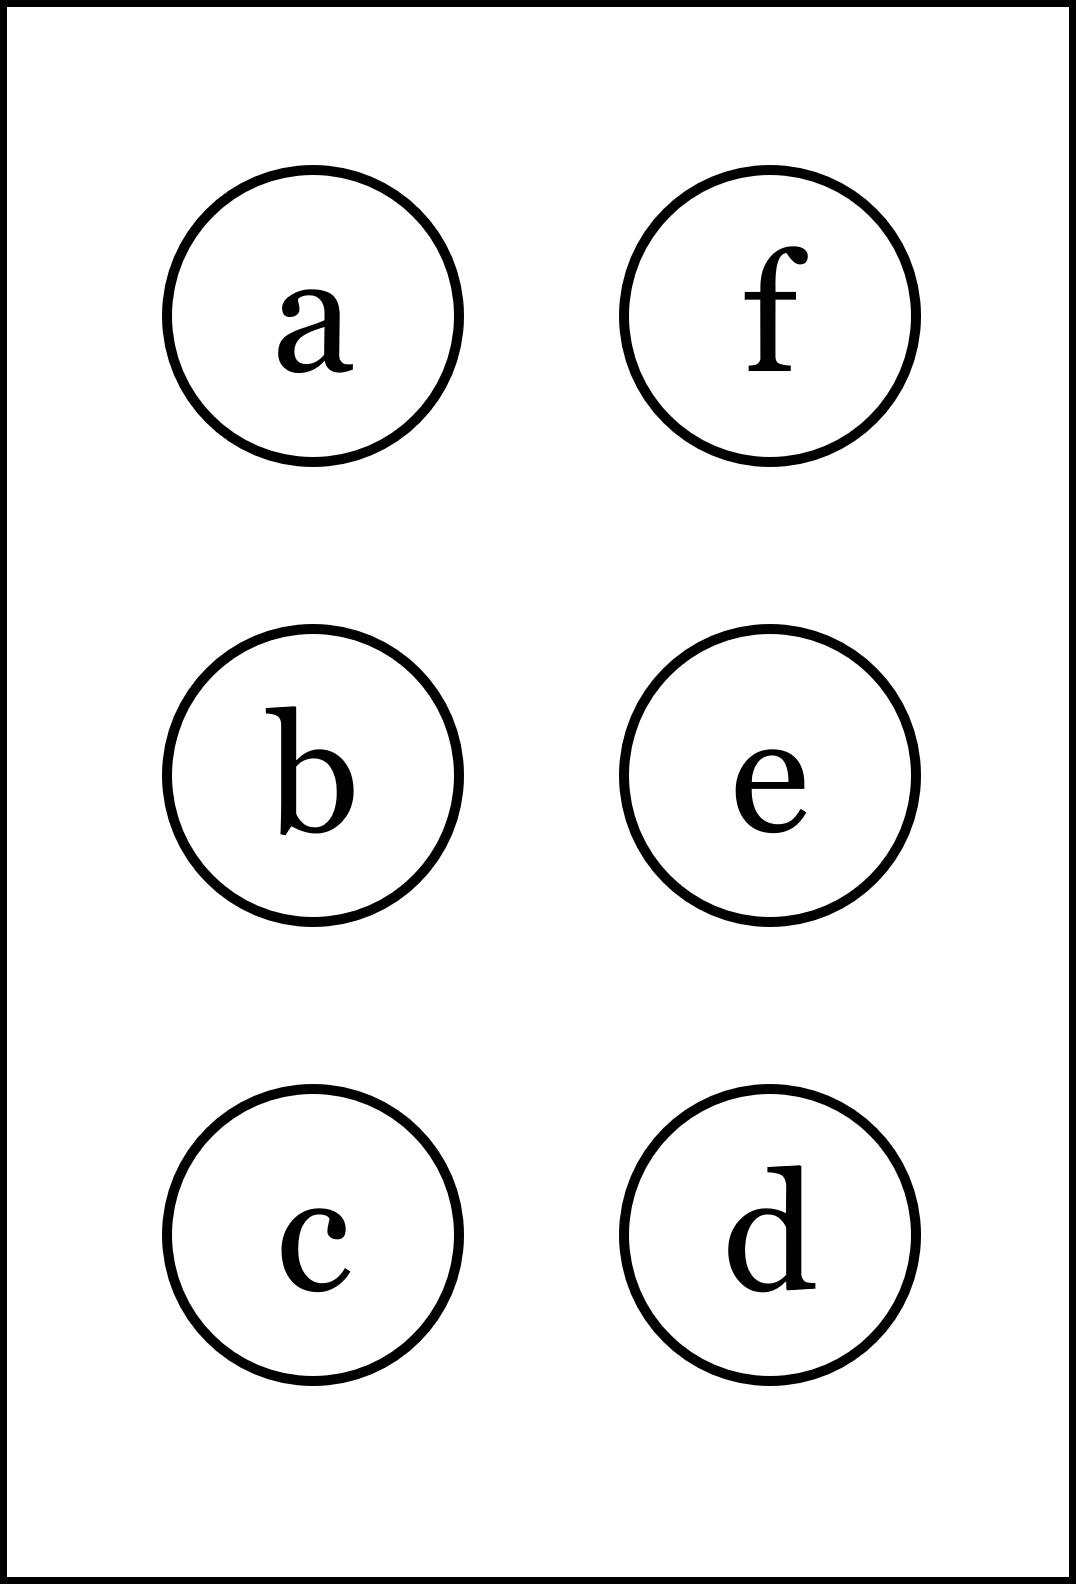
\includegraphics[height=40mm]{../images/braille.png}
{\small Písmeno Braillovej abecedy}
\end{center}
\end{minipage}
\end{center}
\end{minipage}
&
\begin{minipage}[c][104.5mm][t]{0.5\linewidth}
\begin{center}
\vspace{7mm}
{\huge Derivácie, skupina \textit{Zeta $\zeta$} -\romannumeral4}\\[5mm]
\textit{Meno:}\phantom{xxxxxxxxxxxxxxxxxxxxxxxxxxxxxxxxxxxxxxxxxxxxxxxxxxxxxxxxxxxxxxxxx}\\[5mm]
\begin{minipage}{0.95\linewidth}
\begin{center}
\textbf{Vypočítej derivace.} Pokud se výsledky shodují s těmi za otazníky,\\tak napravo obarvi příslušející kroužek načerno. \textbf{Spolu odevzdejte výsledné slovo}.
\end{center}
\end{minipage}
\\[1mm]
\begin{minipage}{0.79\linewidth}
\begin{center}
\begin{varwidth}{\linewidth}
\begin{enumerate}
\normalsize
\item $5x^4-5x^3+9x^2+2x-7$\quad \dotfill\; ???\;\dotfill \quad $5x^3-5x^2+9x+2$
\item $\cfrac{2x^2+2x+3}{5x+2}$\quad \dotfill\; ???\;\dotfill \quad $\cfrac{10x^2+8x-11}{25x^2+20x+4}$
\item $\frac{6}{x}\sqrt{3x-3}$\quad \dotfill\; ???\;\dotfill \quad $\frac{-18x+36}{x^2 \sqrt{\smash[b]{3x-3}}}$
\item $e^{x^2-x-6}$\quad \dotfill\; ???\;\dotfill \quad $e^{x^2-x-6}$
\item $\ln{\left(\frac{3x+1}{x-1}\right)}$\quad \dotfill\; ???\;\dotfill \quad $\frac{3}{3x+1}-\frac{1}{x-1}$
\item $\frac{e^{7x-3}}{-3x+1}$\quad \dotfill\; ???\;\dotfill \quad $\frac{-21x+10}{(-3x+1)^2}e^{7x-3}$
\end{enumerate}
\end{varwidth}
\end{center}
\end{minipage}
\begin{minipage}{0.20\linewidth}
\begin{center}
{\Huge\bfseries 4.} \\[2mm]
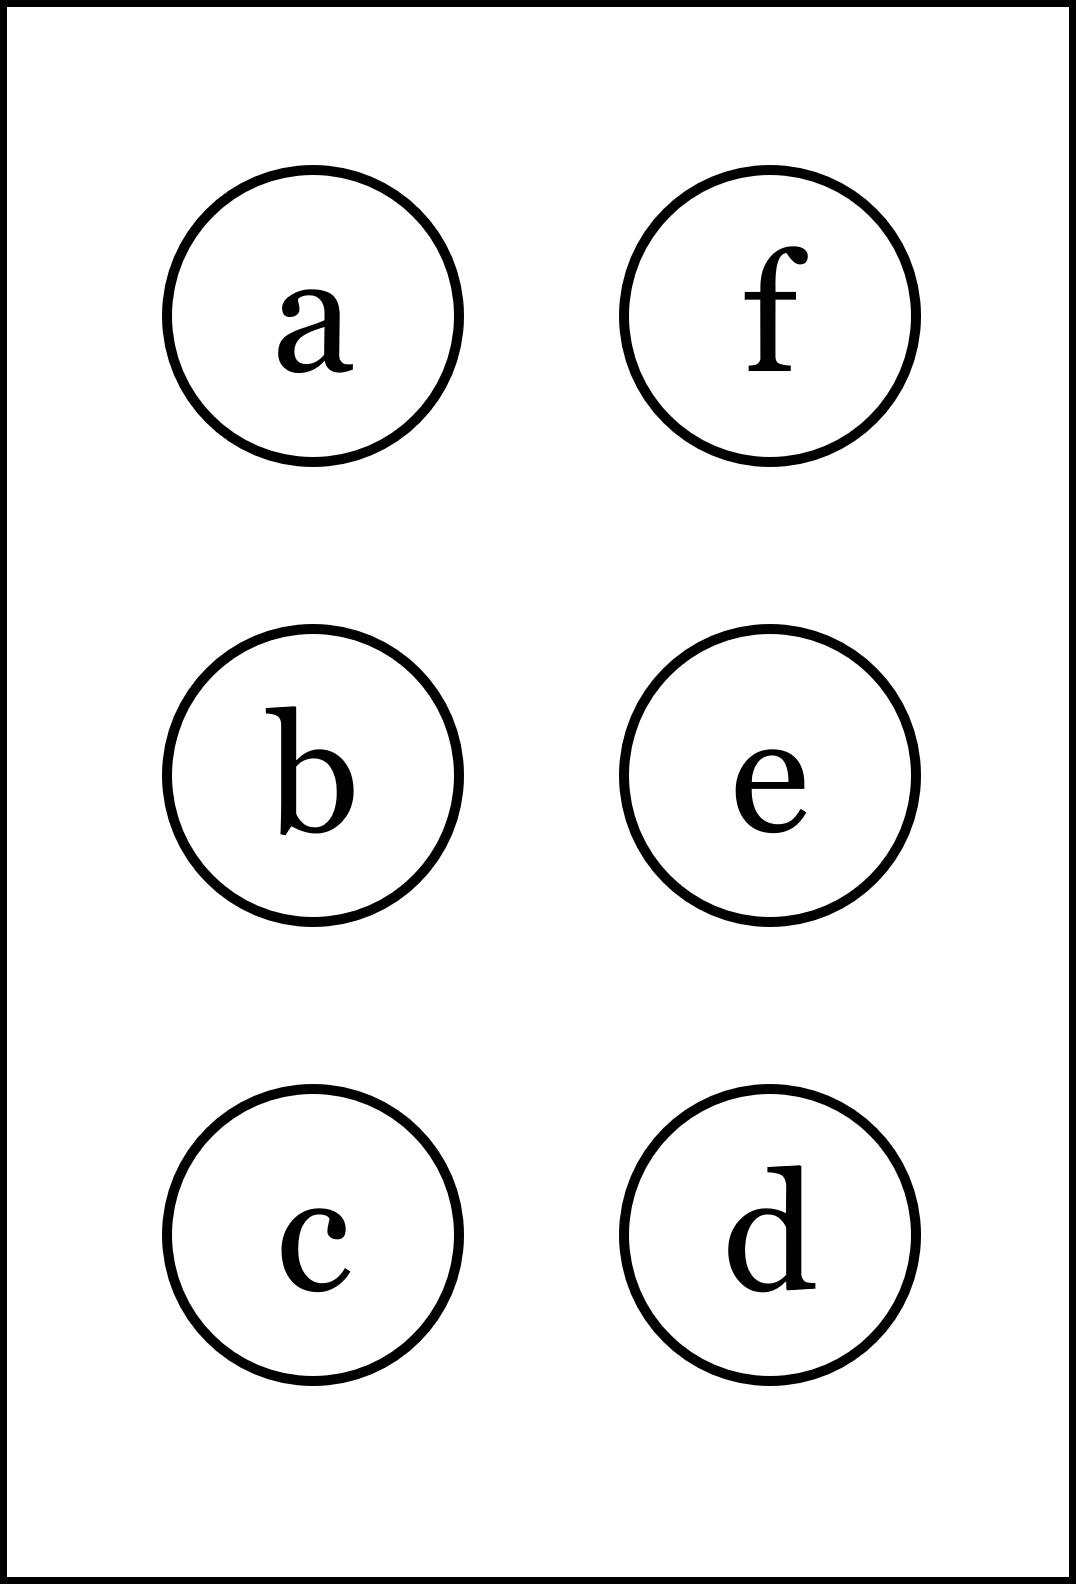
\includegraphics[height=40mm]{../images/braille.png}
{\small Písmeno Braillovej abecedy}
\end{center}
\end{minipage}
\end{center}
\end{minipage}
%
\end{tabular}
\newpage
\thispagestyle{empty}
\begin{tabular}{c:c}
\begin{minipage}[c][104.5mm][t]{0.5\linewidth}
\begin{center}
\vspace{7mm}
{\huge Derivácie, skupina \textit{Eta $\eta$} -\romannumeral1}\\[5mm]
\textit{Meno:}\phantom{xxxxxxxxxxxxxxxxxxxxxxxxxxxxxxxxxxxxxxxxxxxxxxxxxxxxxxxxxxxxxxxxx}\\[5mm]
\begin{minipage}{0.95\linewidth}
\begin{center}
\textbf{Vypočítej derivace.} Pokud se výsledky shodují s těmi za otazníky,\\tak napravo obarvi příslušející kroužek načerno. \textbf{Spolu odevzdejte výsledné slovo}.
\end{center}
\end{minipage}
\\[1mm]
\begin{minipage}{0.79\linewidth}
\begin{center}
\begin{varwidth}{\linewidth}
\begin{enumerate}
\normalsize
\item $7x^4+4x^3-4x^2-2x+1$\quad \dotfill\; ???\;\dotfill \quad $28x^3+12x^2-8x-2$
\item $\cfrac{4x^2+x-2}{-4x+4}$\quad \dotfill\; ???\;\dotfill \quad $\cfrac{-16x^2-32x-4}{16x^2-32x+16}$
\item $\frac{-1}{x}\sqrt{-3x+4}$\quad \dotfill\; ???\;\dotfill \quad $\frac{-3x+8}{2x^2 \sqrt{\smash[b]{-3x+4}}}$
\item $e^{-x^2+6x+3}$\quad \dotfill\; ???\;\dotfill \quad $(-2x+6)e^{-x^2+6x+3}$
\item $\ln{\left(\frac{-2x+8}{3x+5}\right)}$\quad \dotfill\; ???\;\dotfill \quad $\frac{-2}{-2x+8}+\frac{3}{3x+5}$
\item $\frac{e^{-x+3}}{-x-5}$\quad \dotfill\; ???\;\dotfill \quad $\frac{-x+6}{(-x-5)^2}e^{-x+3}$
\end{enumerate}
\end{varwidth}
\end{center}
\end{minipage}
\begin{minipage}{0.20\linewidth}
\begin{center}
{\Huge\bfseries 1.} \\[2mm]
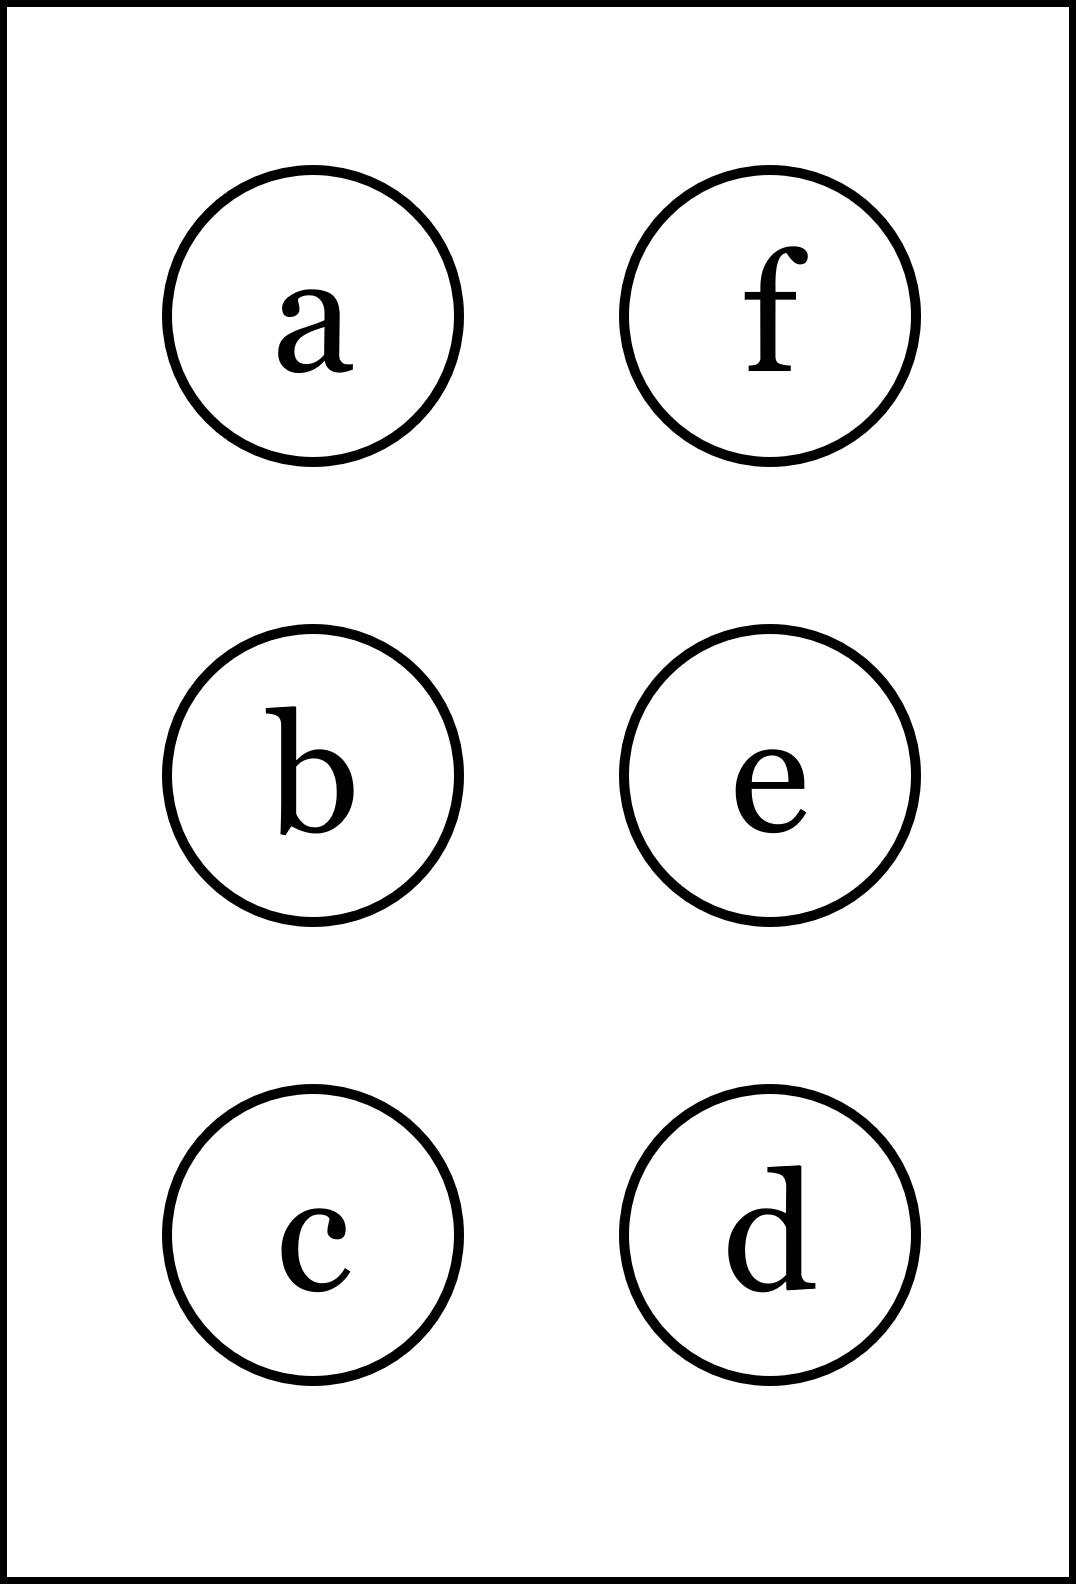
\includegraphics[height=40mm]{../images/braille.png}
{\small Písmeno Braillovej abecedy}
\end{center}
\end{minipage}
\end{center}
\end{minipage}
&
\begin{minipage}[c][104.5mm][t]{0.5\linewidth}
\begin{center}
\vspace{7mm}
{\huge Derivácie, skupina \textit{Eta $\eta$} -\romannumeral2}\\[5mm]
\textit{Meno:}\phantom{xxxxxxxxxxxxxxxxxxxxxxxxxxxxxxxxxxxxxxxxxxxxxxxxxxxxxxxxxxxxxxxxx}\\[5mm]
\begin{minipage}{0.95\linewidth}
\begin{center}
\textbf{Vypočítej derivace.} Pokud se výsledky shodují s těmi za otazníky,\\tak napravo obarvi příslušející kroužek načerno. \textbf{Spolu odevzdejte výsledné slovo}.
\end{center}
\end{minipage}
\\[1mm]
\begin{minipage}{0.79\linewidth}
\begin{center}
\begin{varwidth}{\linewidth}
\begin{enumerate}
\normalsize
\item $-3x^4-2x^3+8x^2+3x+3$\quad \dotfill\; ???\;\dotfill \quad $-12x^3-6x^2+16x+3$
\item $\cfrac{2x^2+6x-4}{6x-1}$\quad \dotfill\; ???\;\dotfill \quad $\cfrac{12x^2-4x+18}{36x^2-12x+1}$
\item $\frac{1}{x}\sqrt{-6x+5}$\quad \dotfill\; ???\;\dotfill \quad $\frac{6x-10}{2x^2 \sqrt{\smash[b]{-6x+5}}}$
\item $e^{-9x^2-7x+4}$\quad \dotfill\; ???\;\dotfill \quad $e^{-9x^2-7x+4}$
\item $\ln{\left(\frac{-7x+7}{5x-3}\right)}$\quad \dotfill\; ???\;\dotfill \quad $\frac{-7}{-7x+7}-\frac{5}{5x-3}$
\item $\frac{e^{-4x-2}}{-2x+6}$\quad \dotfill\; ???\;\dotfill \quad $\frac{-8x-22}{(-2x+6)^2}e^{-4x-2}$
\end{enumerate}
\end{varwidth}
\end{center}
\end{minipage}
\begin{minipage}{0.20\linewidth}
\begin{center}
{\Huge\bfseries 2.} \\[2mm]
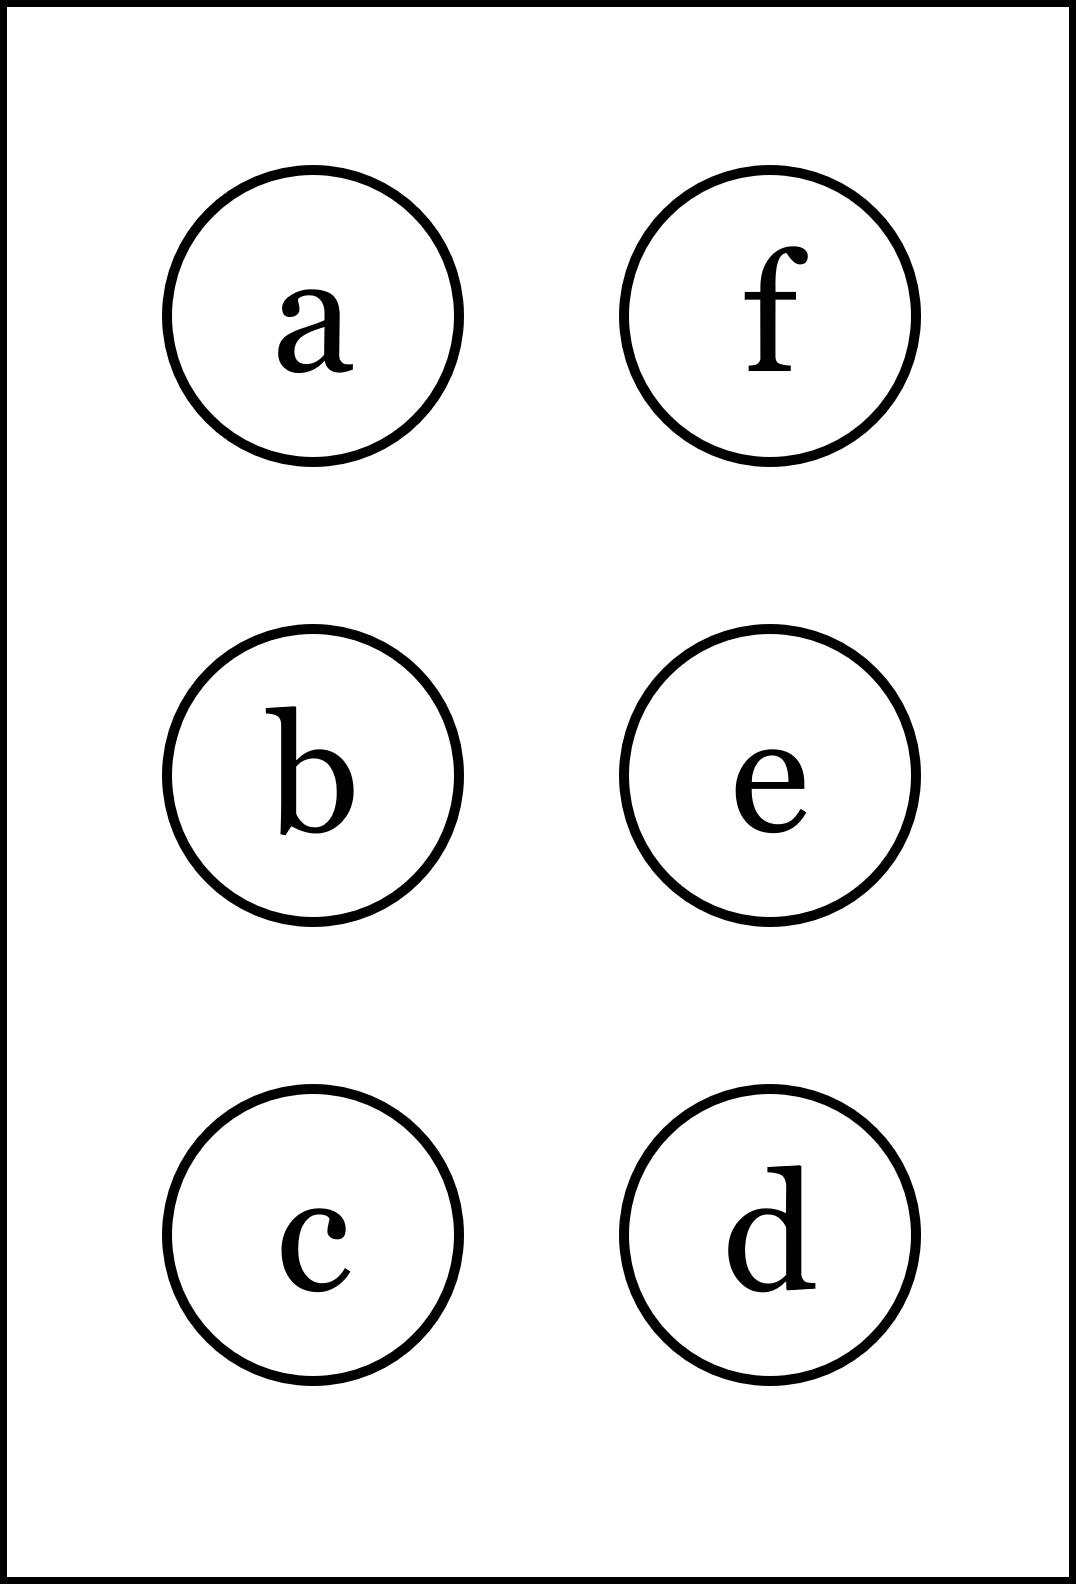
\includegraphics[height=40mm]{../images/braille.png}
{\small Písmeno Braillovej abecedy}
\end{center}
\end{minipage}
\end{center}
\end{minipage}
\\ \hdashline
\begin{minipage}[c][104.5mm][t]{0.5\linewidth}
\begin{center}
\vspace{7mm}
{\huge Derivácie, skupina \textit{Eta $\eta$} -\romannumeral3}\\[5mm]
\textit{Meno:}\phantom{xxxxxxxxxxxxxxxxxxxxxxxxxxxxxxxxxxxxxxxxxxxxxxxxxxxxxxxxxxxxxxxxx}\\[5mm]
\begin{minipage}{0.95\linewidth}
\begin{center}
\textbf{Vypočítej derivace.} Pokud se výsledky shodují s těmi za otazníky,\\tak napravo obarvi příslušející kroužek načerno. \textbf{Spolu odevzdejte výsledné slovo}.
\end{center}
\end{minipage}
\\[1mm]
\begin{minipage}{0.79\linewidth}
\begin{center}
\begin{varwidth}{\linewidth}
\begin{enumerate}
\normalsize
\item $-2x^4+5x^3-x^2-4x-2$\quad \dotfill\; ???\;\dotfill \quad $-8x^3+15x^2-2x-4$
\item $\cfrac{-2x^2+4x-4}{-4x-4}$\quad \dotfill\; ???\;\dotfill \quad $\cfrac{8x^2-16x-32}{16x^2+32x+16}$
\item $\frac{-2}{x}\sqrt{2x-3}$\quad \dotfill\; ???\;\dotfill \quad $\frac{4x-12}{2x^2 \sqrt{\smash[b]{2x-3}}}$
\item $e^{x^2+3x+7}$\quad \dotfill\; ???\;\dotfill \quad $e^{x^2+3x+7}$
\item $\ln{\left(\frac{x-1}{2x-6}\right)}$\quad \dotfill\; ???\;\dotfill \quad $\frac{1}{x-1}-\frac{2}{2x-6}$
\item $\frac{e^{9x+1}}{-6x-7}$\quad \dotfill\; ???\;\dotfill \quad $\frac{-54x-57}{(-6x-7)^2}e^{9x+1}$
\end{enumerate}
\end{varwidth}
\end{center}
\end{minipage}
\begin{minipage}{0.20\linewidth}
\begin{center}
{\Huge\bfseries 3.} \\[2mm]
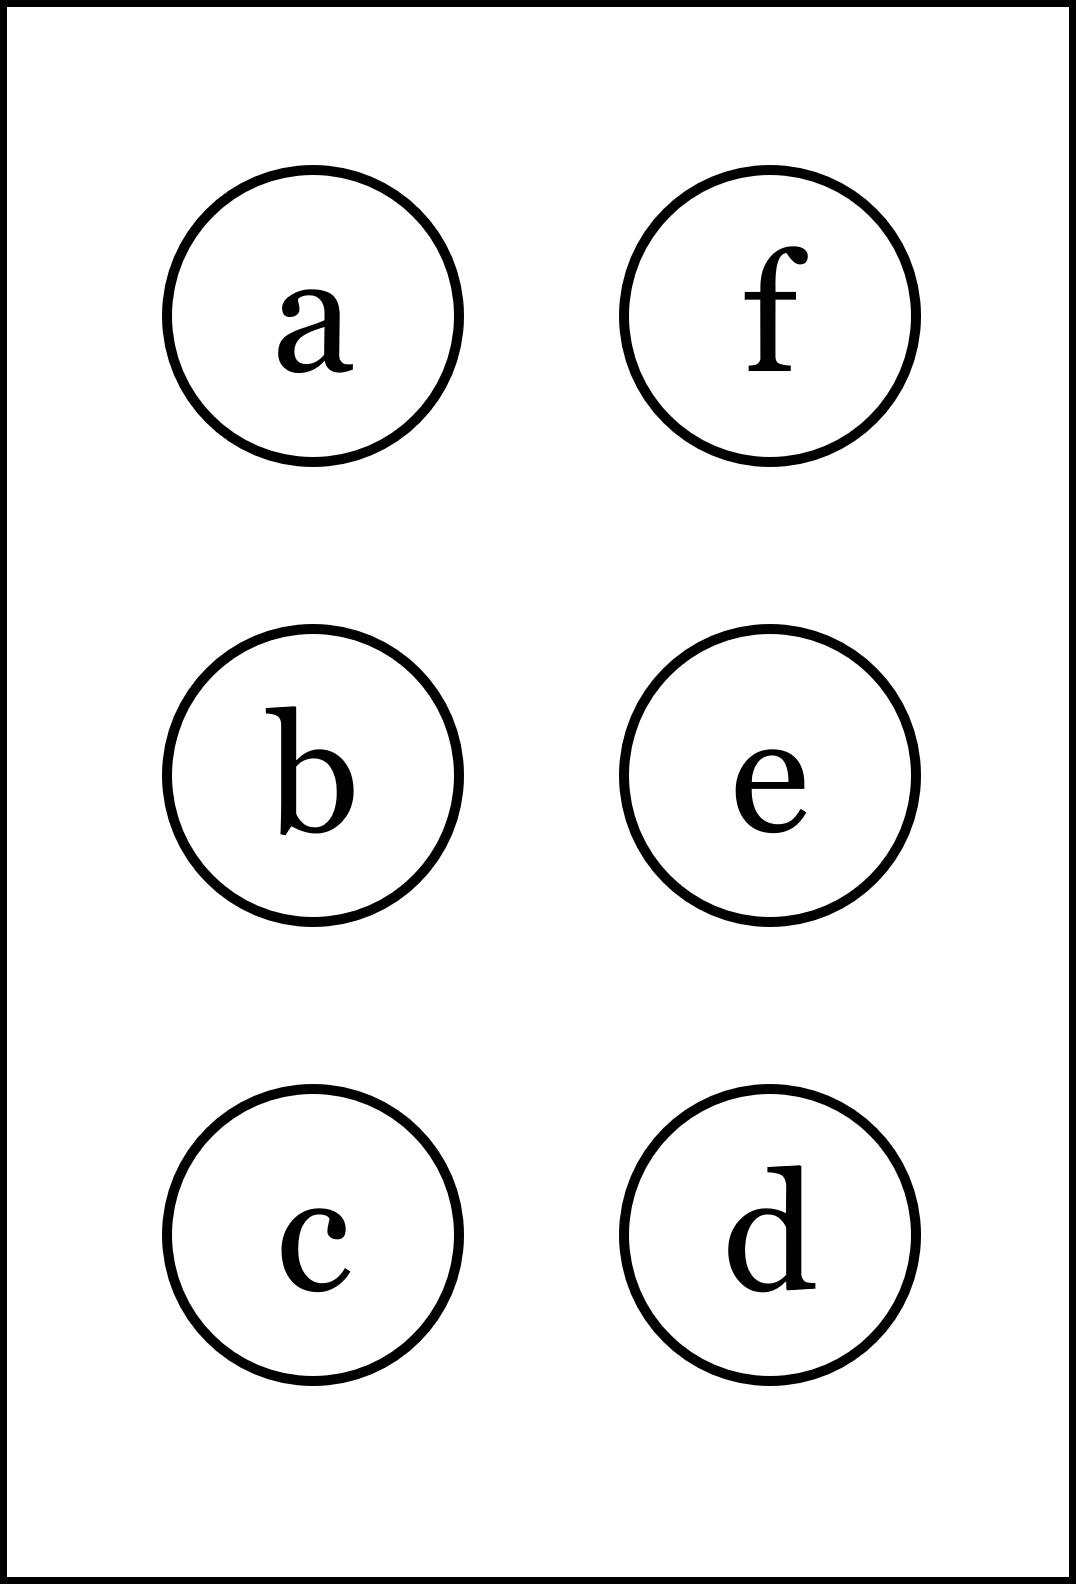
\includegraphics[height=40mm]{../images/braille.png}
{\small Písmeno Braillovej abecedy}
\end{center}
\end{minipage}
\end{center}
\end{minipage}
&
\begin{minipage}[c][104.5mm][t]{0.5\linewidth}
\begin{center}
\vspace{7mm}
{\huge Derivácie, skupina \textit{Eta $\eta$} -\romannumeral4}\\[5mm]
\textit{Meno:}\phantom{xxxxxxxxxxxxxxxxxxxxxxxxxxxxxxxxxxxxxxxxxxxxxxxxxxxxxxxxxxxxxxxxx}\\[5mm]
\begin{minipage}{0.95\linewidth}
\begin{center}
\textbf{Vypočítej derivace.} Pokud se výsledky shodují s těmi za otazníky,\\tak napravo obarvi příslušející kroužek načerno. \textbf{Spolu odevzdejte výsledné slovo}.
\end{center}
\end{minipage}
\\[1mm]
\begin{minipage}{0.79\linewidth}
\begin{center}
\begin{varwidth}{\linewidth}
\begin{enumerate}
\normalsize
\item $-6x^4+2x^3+3x^2-3x+4$\quad \dotfill\; ???\;\dotfill \quad $-24x^3+6x^2+6x-3$
\item $\cfrac{-5x^2+3x+1}{-5x+1}$\quad \dotfill\; ???\;\dotfill \quad $\cfrac{25x^2+10x+8}{25x^2-10x+1}$
\item $\frac{4}{x}\sqrt{5x-5}$\quad \dotfill\; ???\;\dotfill \quad $\frac{-20x+40}{x^2 \sqrt{\smash[b]{5x-5}}}$
\item $e^{3x^2-6x+2}$\quad \dotfill\; ???\;\dotfill \quad $e^{3x^2-6x+2}$
\item $\ln{\left(\frac{8x+2}{3x-9}\right)}$\quad \dotfill\; ???\;\dotfill \quad $\frac{8}{8x+2}+\frac{3}{3x-9}$
\item $\frac{e^{4x-4}}{2x+7}$\quad \dotfill\; ???\;\dotfill \quad $\frac{-8x+26}{(2x+7)^2}e^{4x-4}$
\end{enumerate}
\end{varwidth}
\end{center}
\end{minipage}
\begin{minipage}{0.20\linewidth}
\begin{center}
{\Huge\bfseries 4.} \\[2mm]
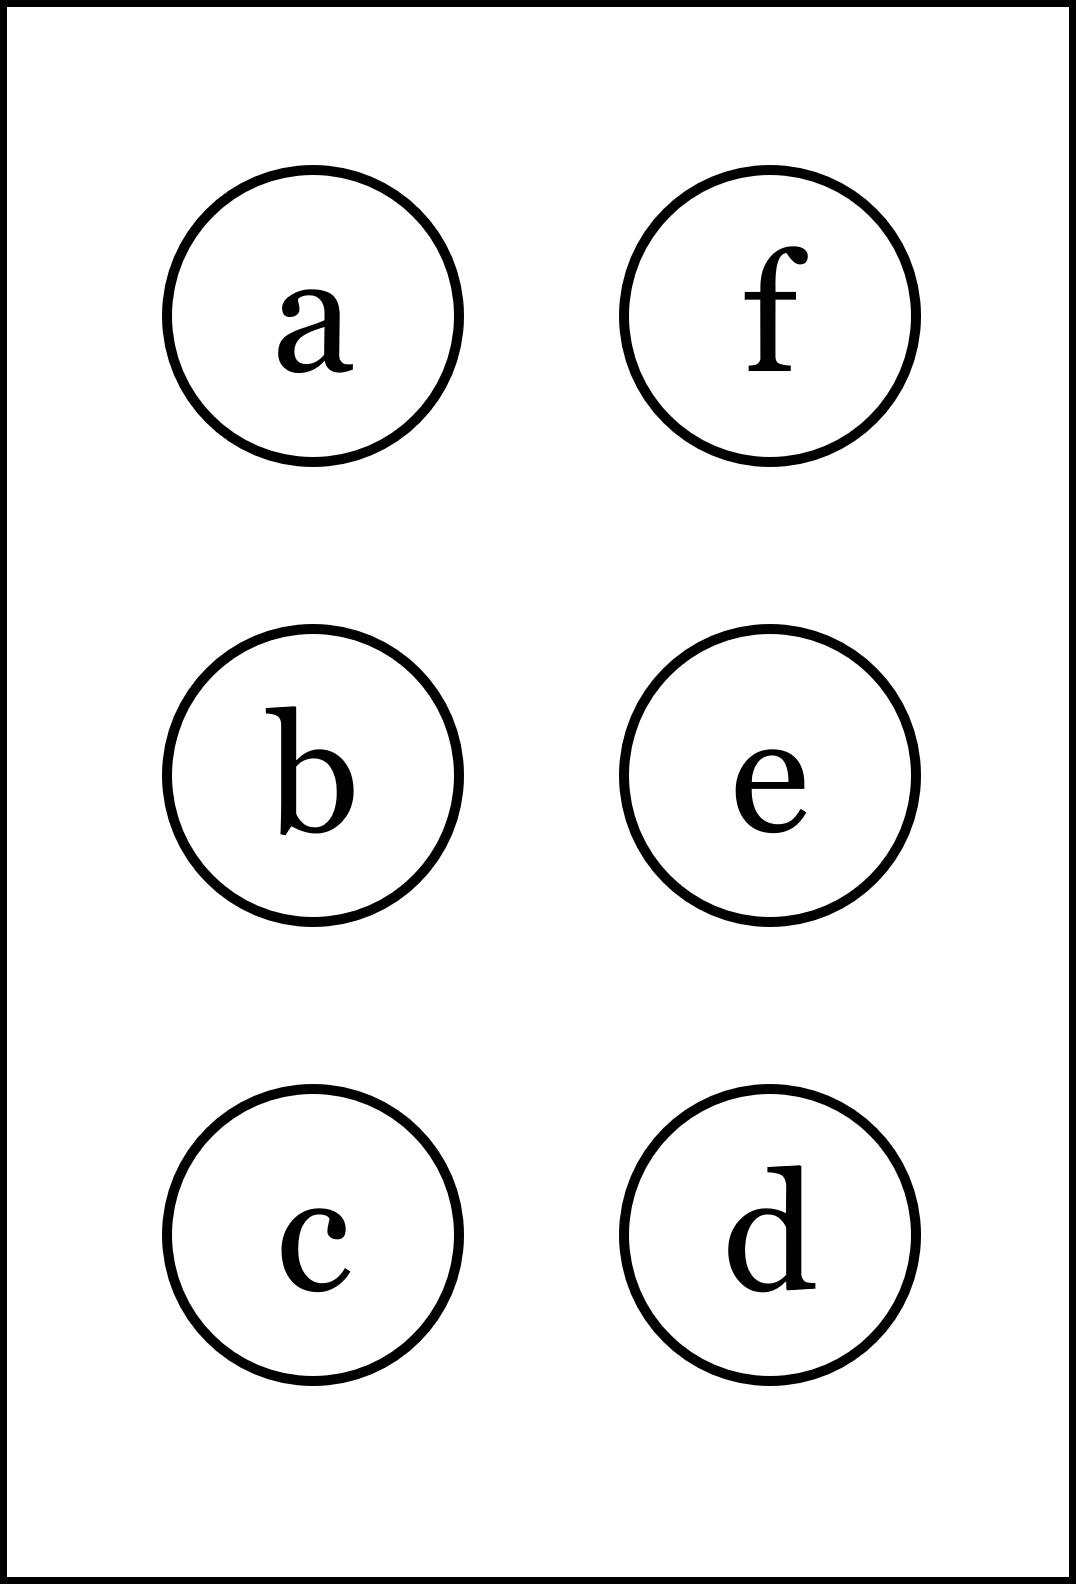
\includegraphics[height=40mm]{../images/braille.png}
{\small Písmeno Braillovej abecedy}
\end{center}
\end{minipage}
\end{center}
\end{minipage}
%
\end{tabular}
\newpage
\thispagestyle{empty}
\begin{tabular}{c:c}
\begin{minipage}[c][104.5mm][t]{0.5\linewidth}
\begin{center}
\vspace{7mm}
{\huge Derivácie, skupina \textit{Theta $\theta$} -\romannumeral1}\\[5mm]
\textit{Meno:}\phantom{xxxxxxxxxxxxxxxxxxxxxxxxxxxxxxxxxxxxxxxxxxxxxxxxxxxxxxxxxxxxxxxxx}\\[5mm]
\begin{minipage}{0.95\linewidth}
\begin{center}
\textbf{Vypočítej derivace.} Pokud se výsledky shodují s těmi za otazníky,\\tak napravo obarvi příslušející kroužek načerno. \textbf{Spolu odevzdejte výsledné slovo}.
\end{center}
\end{minipage}
\\[1mm]
\begin{minipage}{0.79\linewidth}
\begin{center}
\begin{varwidth}{\linewidth}
\begin{enumerate}
\normalsize
\item $-5x^4-9x^3+4x^2-x-6$\quad \dotfill\; ???\;\dotfill \quad $-20x^3-27x^2+8x-1$
\item $\cfrac{2x^2-2x-3}{6x+1}$\quad \dotfill\; ???\;\dotfill \quad $\cfrac{12x^2+4x+16}{36x^2+12x+1}$
\item $\frac{6}{x}\sqrt{2x+5}$\quad \dotfill\; ???\;\dotfill \quad $\frac{-12x-60}{x^2 \sqrt{\smash[b]{2x+5}}}$
\item $e^{-3x^2+2x-3}$\quad \dotfill\; ???\;\dotfill \quad $e^{-3x^2+2x-3}$
\item $\ln{\left(\frac{2x-5}{-5x-4}\right)}$\quad \dotfill\; ???\;\dotfill \quad $\frac{2}{2x-5}+\frac{-5}{-5x-4}$
\item $\frac{e^{5x+3}}{x+6}$\quad \dotfill\; ???\;\dotfill \quad $\frac{5x+29}{(x+6)^2}e^{5x+3}$
\end{enumerate}
\end{varwidth}
\end{center}
\end{minipage}
\begin{minipage}{0.20\linewidth}
\begin{center}
{\Huge\bfseries 1.} \\[2mm]
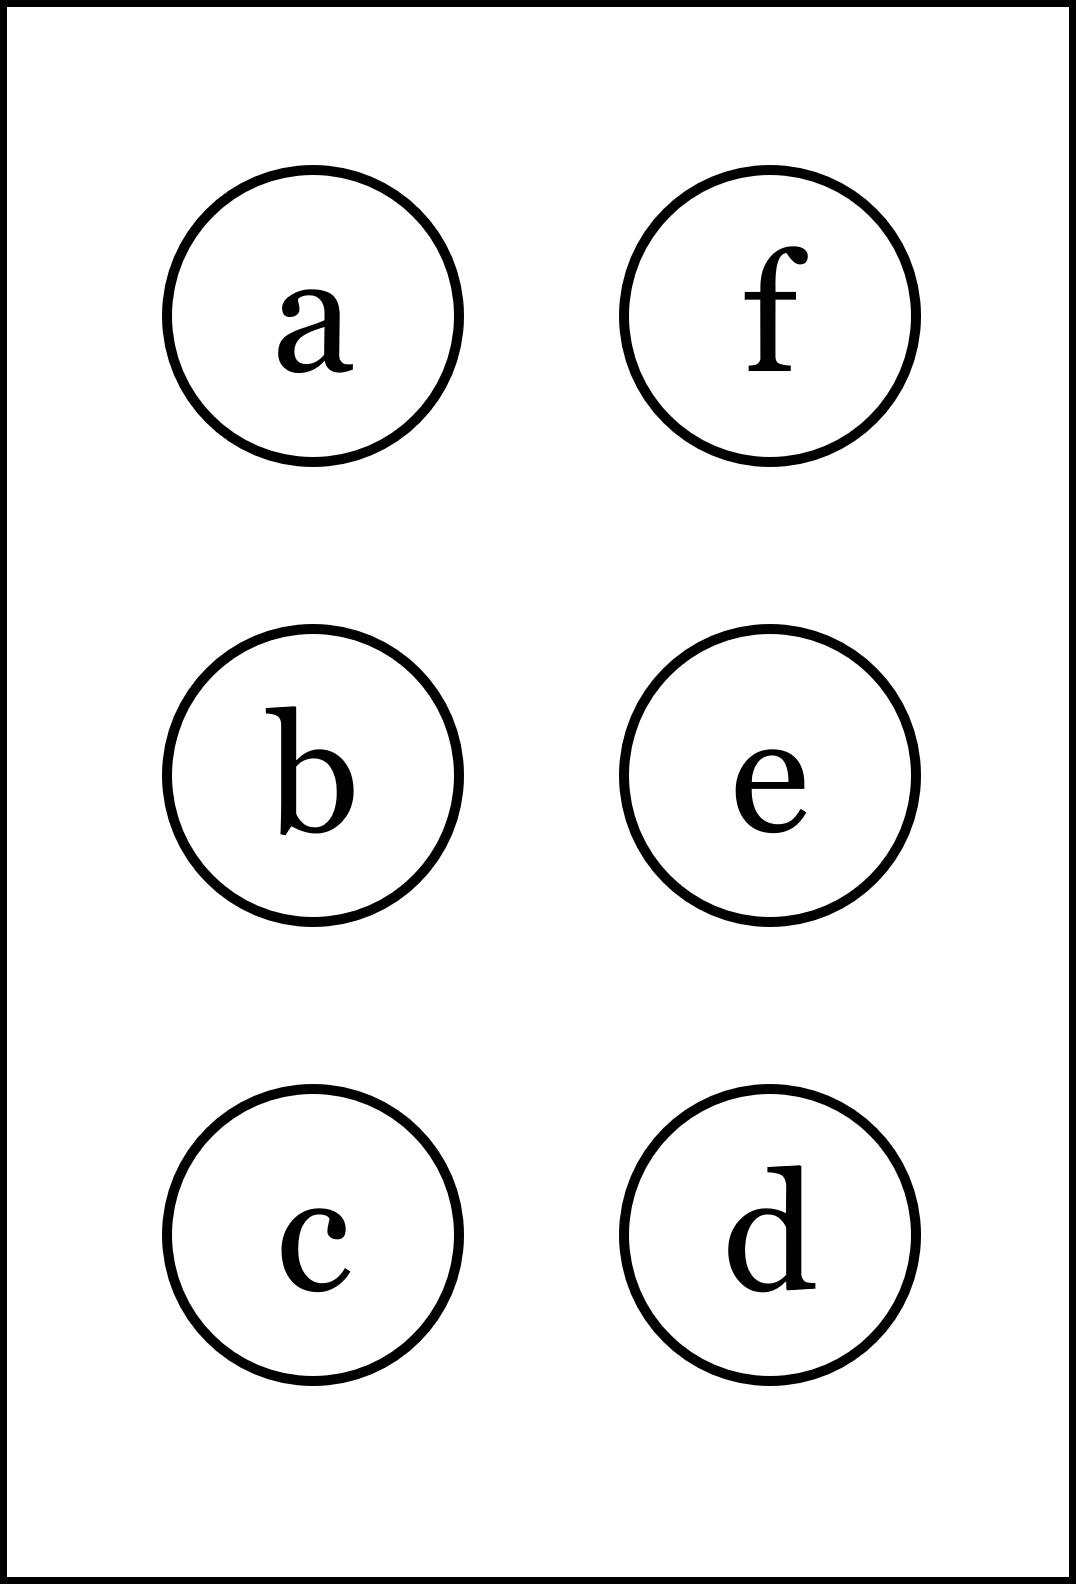
\includegraphics[height=40mm]{../images/braille.png}
{\small Písmeno Braillovej abecedy}
\end{center}
\end{minipage}
\end{center}
\end{minipage}
&
\begin{minipage}[c][104.5mm][t]{0.5\linewidth}
\begin{center}
\vspace{7mm}
{\huge Derivácie, skupina \textit{Theta $\theta$} -\romannumeral2}\\[5mm]
\textit{Meno:}\phantom{xxxxxxxxxxxxxxxxxxxxxxxxxxxxxxxxxxxxxxxxxxxxxxxxxxxxxxxxxxxxxxxxx}\\[5mm]
\begin{minipage}{0.95\linewidth}
\begin{center}
\textbf{Vypočítej derivace.} Pokud se výsledky shodují s těmi za otazníky,\\tak napravo obarvi příslušející kroužek načerno. \textbf{Spolu odevzdejte výsledné slovo}.
\end{center}
\end{minipage}
\\[1mm]
\begin{minipage}{0.79\linewidth}
\begin{center}
\begin{varwidth}{\linewidth}
\begin{enumerate}
\normalsize
\item $4x^4+5x^3-7x^2+2x-2$\quad \dotfill\; ???\;\dotfill \quad $4x^3+5x^2-7x+2$
\item $\cfrac{-x^2-x+3}{-3x-3}$\quad \dotfill\; ???\;\dotfill \quad $\cfrac{3x^2-6x+12}{9x^2+18x+9}$
\item $\frac{1}{x}\sqrt{-4x-4}$\quad \dotfill\; ???\;\dotfill \quad $\frac{4x+8}{2x^2 \sqrt{\smash[b]{-4x-4}}}$
\item $e^{3x^2+5x-5}$\quad \dotfill\; ???\;\dotfill \quad $e^{3x^2+5x-5}$
\item $\ln{\left(\frac{-4x+3}{-2x-1}\right)}$\quad \dotfill\; ???\;\dotfill \quad $\frac{-4}{-4x+3}+\frac{-2}{-2x-1}$
\item $\frac{e^{x+2}}{-7x-2}$\quad \dotfill\; ???\;\dotfill \quad $\frac{-7x+5}{(-7x-2)^2}e^{x+2}$
\end{enumerate}
\end{varwidth}
\end{center}
\end{minipage}
\begin{minipage}{0.20\linewidth}
\begin{center}
{\Huge\bfseries 2.} \\[2mm]
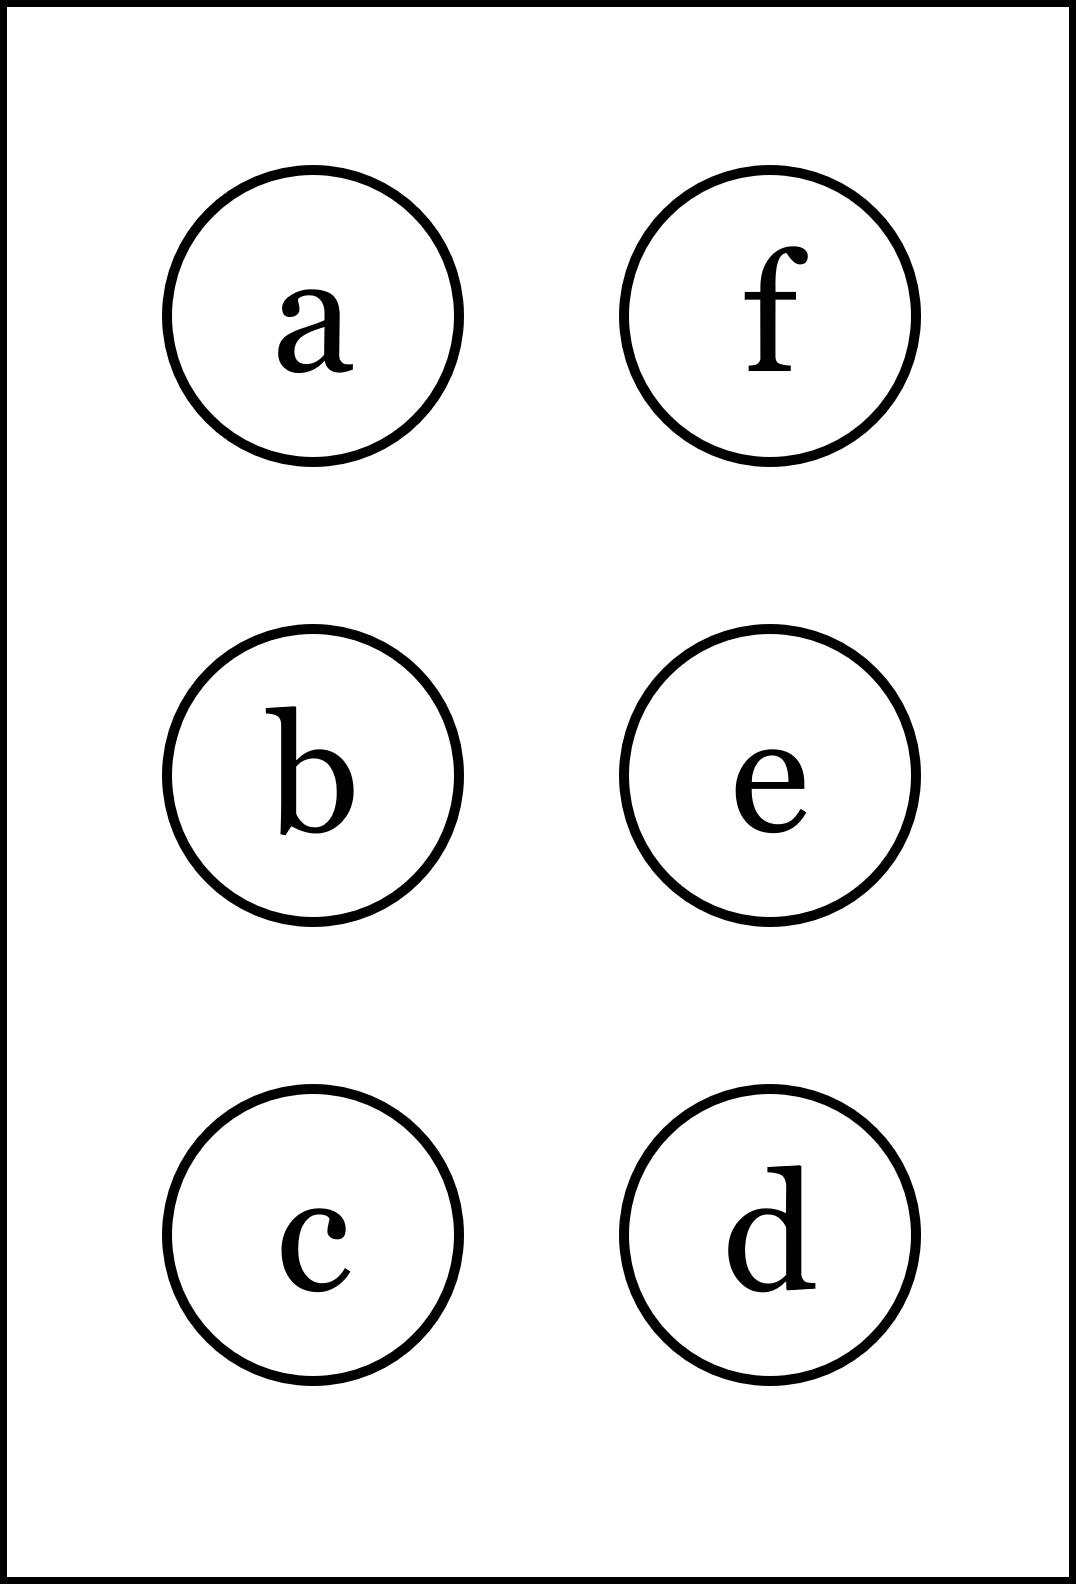
\includegraphics[height=40mm]{../images/braille.png}
{\small Písmeno Braillovej abecedy}
\end{center}
\end{minipage}
\end{center}
\end{minipage}
\\ \hdashline
\begin{minipage}[c][104.5mm][t]{0.5\linewidth}
\begin{center}
\vspace{7mm}
{\huge Derivácie, skupina \textit{Theta $\theta$} -\romannumeral3}\\[5mm]
\textit{Meno:}\phantom{xxxxxxxxxxxxxxxxxxxxxxxxxxxxxxxxxxxxxxxxxxxxxxxxxxxxxxxxxxxxxxxxx}\\[5mm]
\begin{minipage}{0.95\linewidth}
\begin{center}
\textbf{Vypočítej derivace.} Pokud se výsledky shodují s těmi za otazníky,\\tak napravo obarvi příslušející kroužek načerno. \textbf{Spolu odevzdejte výsledné slovo}.
\end{center}
\end{minipage}
\\[1mm]
\begin{minipage}{0.79\linewidth}
\begin{center}
\begin{varwidth}{\linewidth}
\begin{enumerate}
\normalsize
\item $-6x^4-4x^3-4x^2-7x-2$\quad \dotfill\; ???\;\dotfill \quad $-24x^3-12x^2-8x-7$
\item $\cfrac{2x^2-x-4}{-4x+3}$\quad \dotfill\; ???\;\dotfill \quad $\cfrac{-8x^2-12x-19}{16x^2-24x+9}$
\item $\frac{-1}{x}\sqrt{x+9}$\quad \dotfill\; ???\;\dotfill \quad $\frac{x+18}{2x^2 \sqrt{\smash[b]{x+9}}}$
\item $e^{-4x^2+4x-6}$\quad \dotfill\; ???\;\dotfill \quad $e^{-4x^2+4x-6}$
\item $\ln{\left(\frac{7x-6}{-x+3}\right)}$\quad \dotfill\; ???\;\dotfill \quad $\frac{7}{7x-6}+\frac{-1}{-x+3}$
\item $\frac{e^{-6x-1}}{2x-5}$\quad \dotfill\; ???\;\dotfill \quad $\frac{+12x+28}{(2x-5)^2}e^{-6x-1}$
\end{enumerate}
\end{varwidth}
\end{center}
\end{minipage}
\begin{minipage}{0.20\linewidth}
\begin{center}
{\Huge\bfseries 3.} \\[2mm]
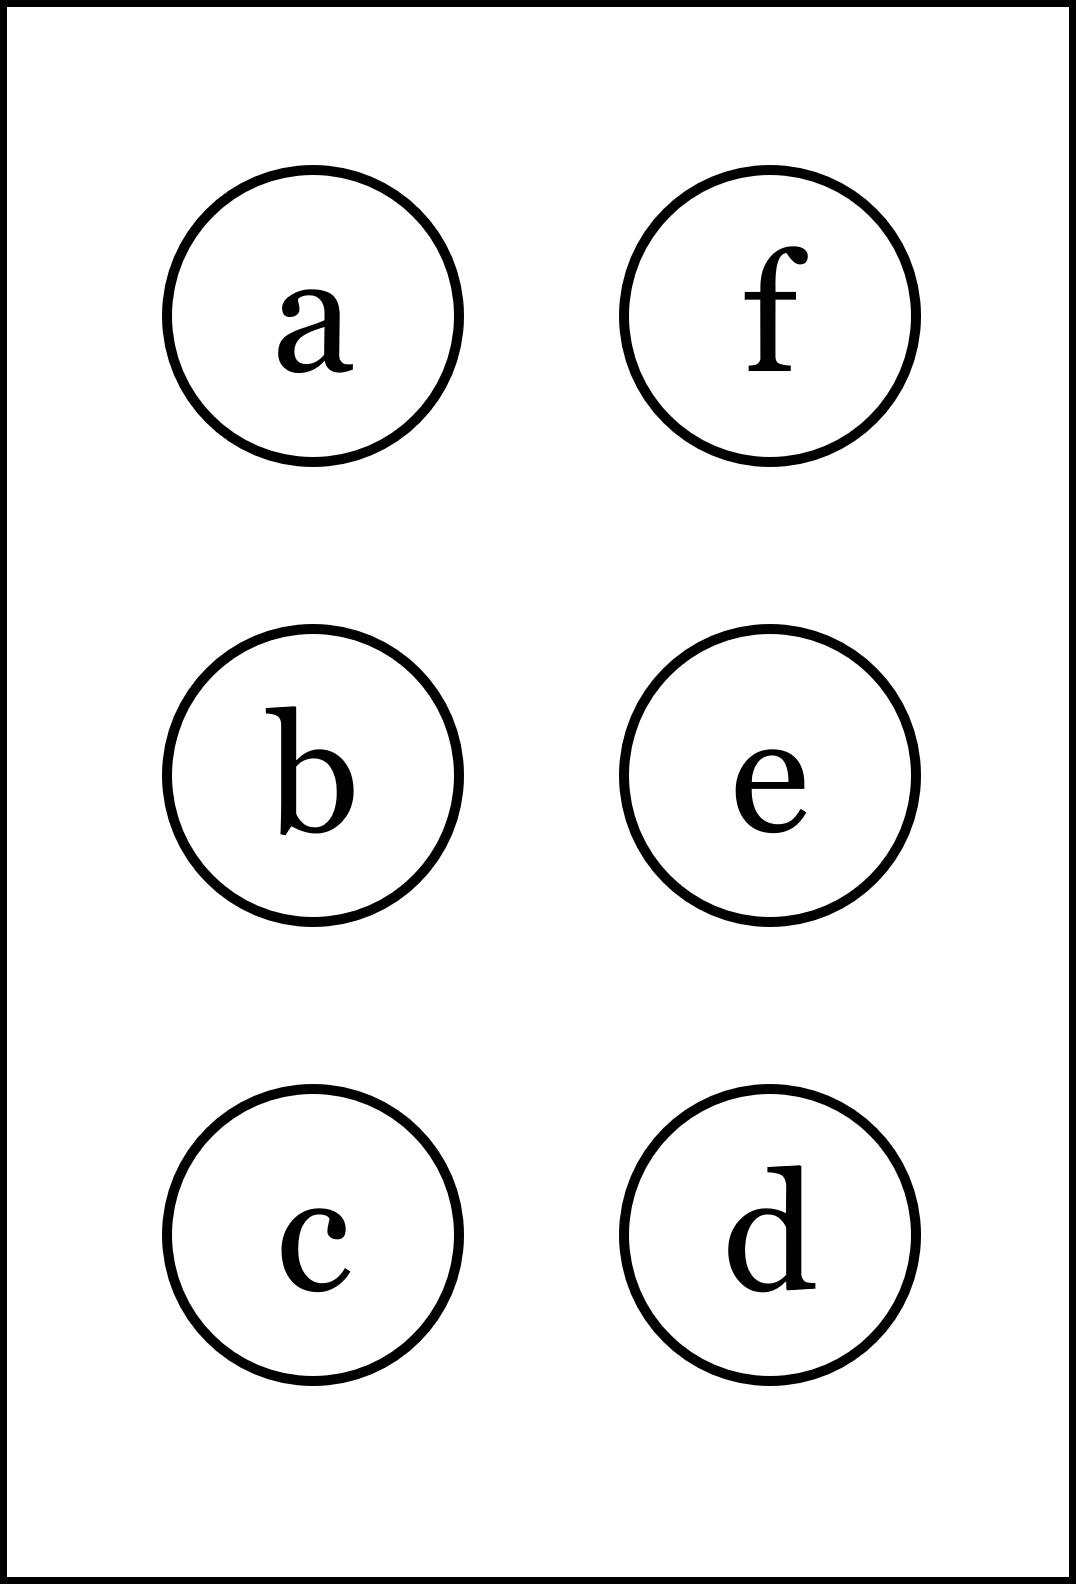
\includegraphics[height=40mm]{../images/braille.png}
{\small Písmeno Braillovej abecedy}
\end{center}
\end{minipage}
\end{center}
\end{minipage}
&
\begin{minipage}[c][104.5mm][t]{0.5\linewidth}
\begin{center}
\vspace{7mm}
{\huge Derivácie, skupina \textit{Theta $\theta$} -\romannumeral4}\\[5mm]
\textit{Meno:}\phantom{xxxxxxxxxxxxxxxxxxxxxxxxxxxxxxxxxxxxxxxxxxxxxxxxxxxxxxxxxxxxxxxxx}\\[5mm]
\begin{minipage}{0.95\linewidth}
\begin{center}
\textbf{Vypočítej derivace.} Pokud se výsledky shodují s těmi za otazníky,\\tak napravo obarvi příslušející kroužek načerno. \textbf{Spolu odevzdejte výsledné slovo}.
\end{center}
\end{minipage}
\\[1mm]
\begin{minipage}{0.79\linewidth}
\begin{center}
\begin{varwidth}{\linewidth}
\begin{enumerate}
\normalsize
\item $6x^4-x^3-6x^2-3x-4$\quad \dotfill\; ???\;\dotfill \quad $24x^3-3x^2-12x-3$
\item $\cfrac{2x^2+5x-3}{2x-4}$\quad \dotfill\; ???\;\dotfill \quad $\cfrac{4x^2+16x-14}{4x^2-16x+16}$
\item $\frac{-3}{x}\sqrt{7x-5}$\quad \dotfill\; ???\;\dotfill \quad $\frac{21x-30}{2x^2 \sqrt{\smash[b]{7x-5}}}$
\item $e^{-5x^2+9x+2}$\quad \dotfill\; ???\;\dotfill \quad $(-10x+9)e^{-5x^2+9x+2}$
\item $\ln{\left(\frac{2x-7}{4x+4}\right)}$\quad \dotfill\; ???\;\dotfill \quad $\frac{2}{2x-7}-\frac{4}{4x+4}$
\item $\frac{e^{-x+5}}{-x+2}$\quad \dotfill\; ???\;\dotfill \quad $\frac{x-1}{(-x+2)^2}e^{-x+5}$
\end{enumerate}
\end{varwidth}
\end{center}
\end{minipage}
\begin{minipage}{0.20\linewidth}
\begin{center}
{\Huge\bfseries 4.} \\[2mm]
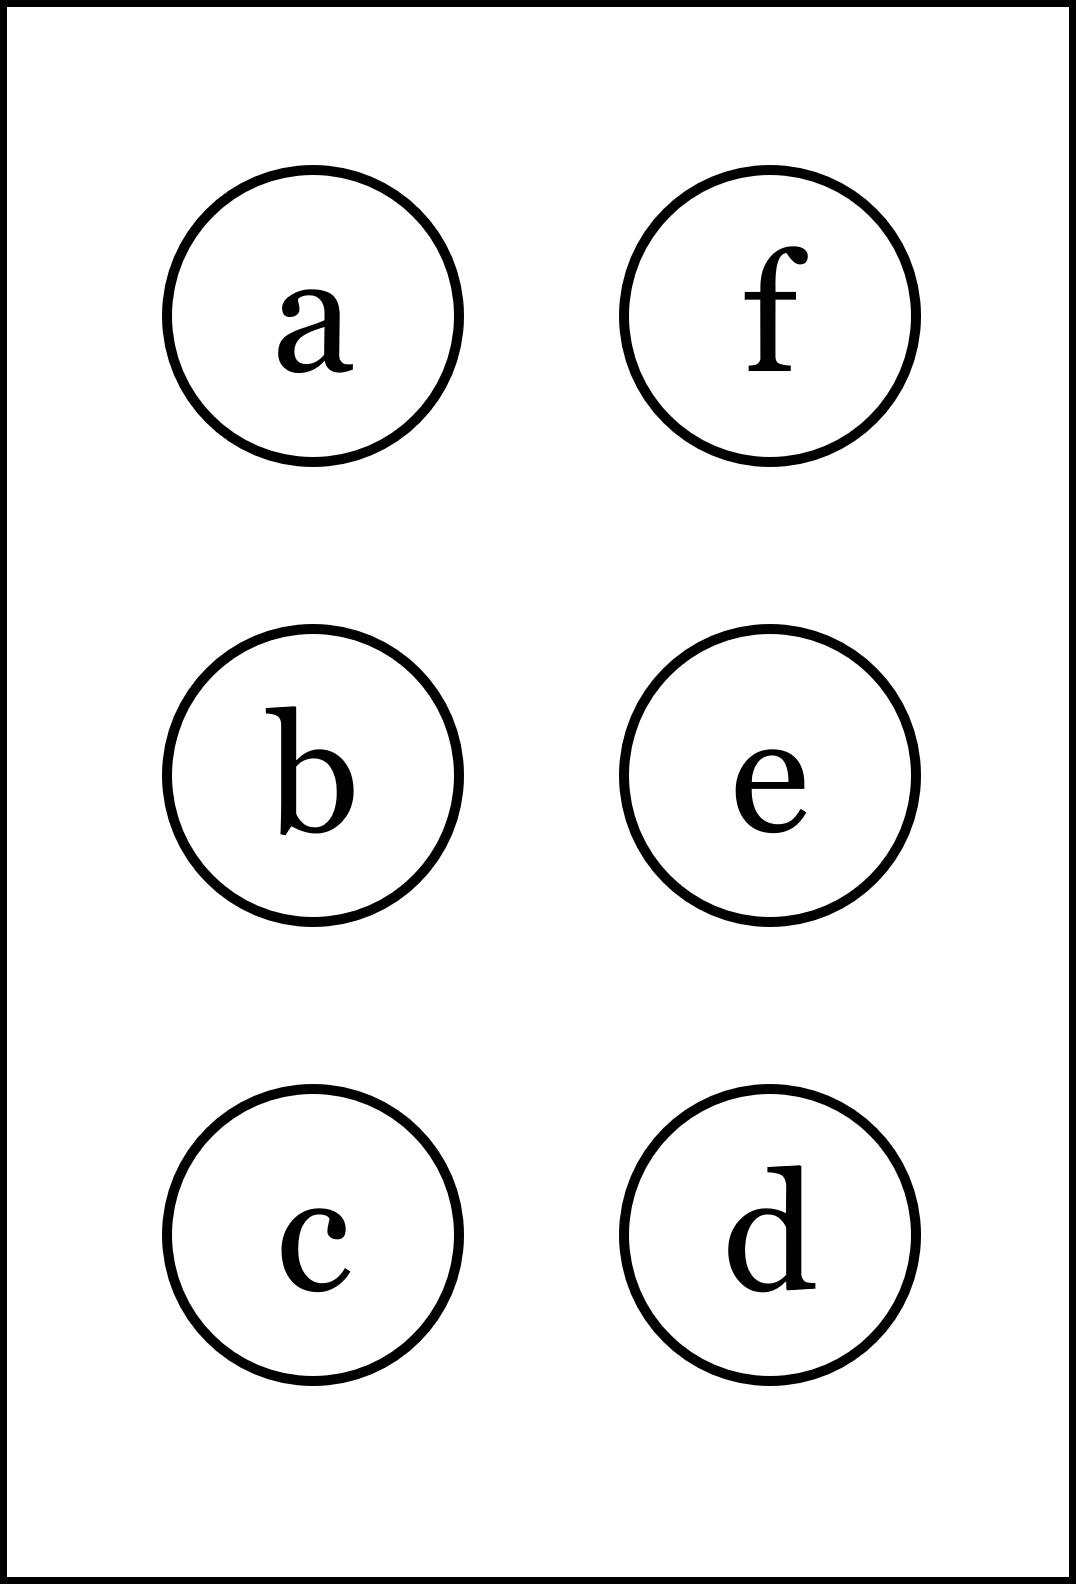
\includegraphics[height=40mm]{../images/braille.png}
{\small Písmeno Braillovej abecedy}
\end{center}
\end{minipage}
\end{center}
\end{minipage}
%
\end{tabular}
\newpage
\thispagestyle{empty}
\begin{tabular}{c:c}
\begin{minipage}[c][104.5mm][t]{0.5\linewidth}
\begin{center}
\vspace{7mm}
{\huge Derivácie, skupina \textit{Iota $\iota$} -\romannumeral1}\\[5mm]
\textit{Meno:}\phantom{xxxxxxxxxxxxxxxxxxxxxxxxxxxxxxxxxxxxxxxxxxxxxxxxxxxxxxxxxxxxxxxxx}\\[5mm]
\begin{minipage}{0.95\linewidth}
\begin{center}
\textbf{Vypočítej derivace.} Pokud se výsledky shodují s těmi za otazníky,\\tak napravo obarvi příslušející kroužek načerno. \textbf{Spolu odevzdejte výsledné slovo}.
\end{center}
\end{minipage}
\\[1mm]
\begin{minipage}{0.79\linewidth}
\begin{center}
\begin{varwidth}{\linewidth}
\begin{enumerate}
\normalsize
\item $2x^4-x^3-5x^2-4x+2$\quad \dotfill\; ???\;\dotfill \quad $8x^3-3x^2-10x-4$
\item $\cfrac{3x^2-6x+5}{-3x+2}$\quad \dotfill\; ???\;\dotfill \quad $\cfrac{-9x^2+12x+3}{9x^2-12x+4}$
\item $\frac{-4}{x}\sqrt{3x+9}$\quad \dotfill\; ???\;\dotfill \quad $\frac{12x+72}{2x^2 \sqrt{\smash[b]{3x+9}}}$
\item $e^{3x^2-2x+3}$\quad \dotfill\; ???\;\dotfill \quad $e^{3x^2-2x+3}$
\item $\ln{\left(\frac{-6x-1}{-9x-3}\right)}$\quad \dotfill\; ???\;\dotfill \quad $\frac{-6}{-6x-1}+\frac{-9}{-9x-3}$
\item $\frac{e^{-3x+2}}{-3x-5}$\quad \dotfill\; ???\;\dotfill \quad $\frac{-9x+18}{(-3x-5)^2}e^{-3x+2}$
\end{enumerate}
\end{varwidth}
\end{center}
\end{minipage}
\begin{minipage}{0.20\linewidth}
\begin{center}
{\Huge\bfseries 1.} \\[2mm]
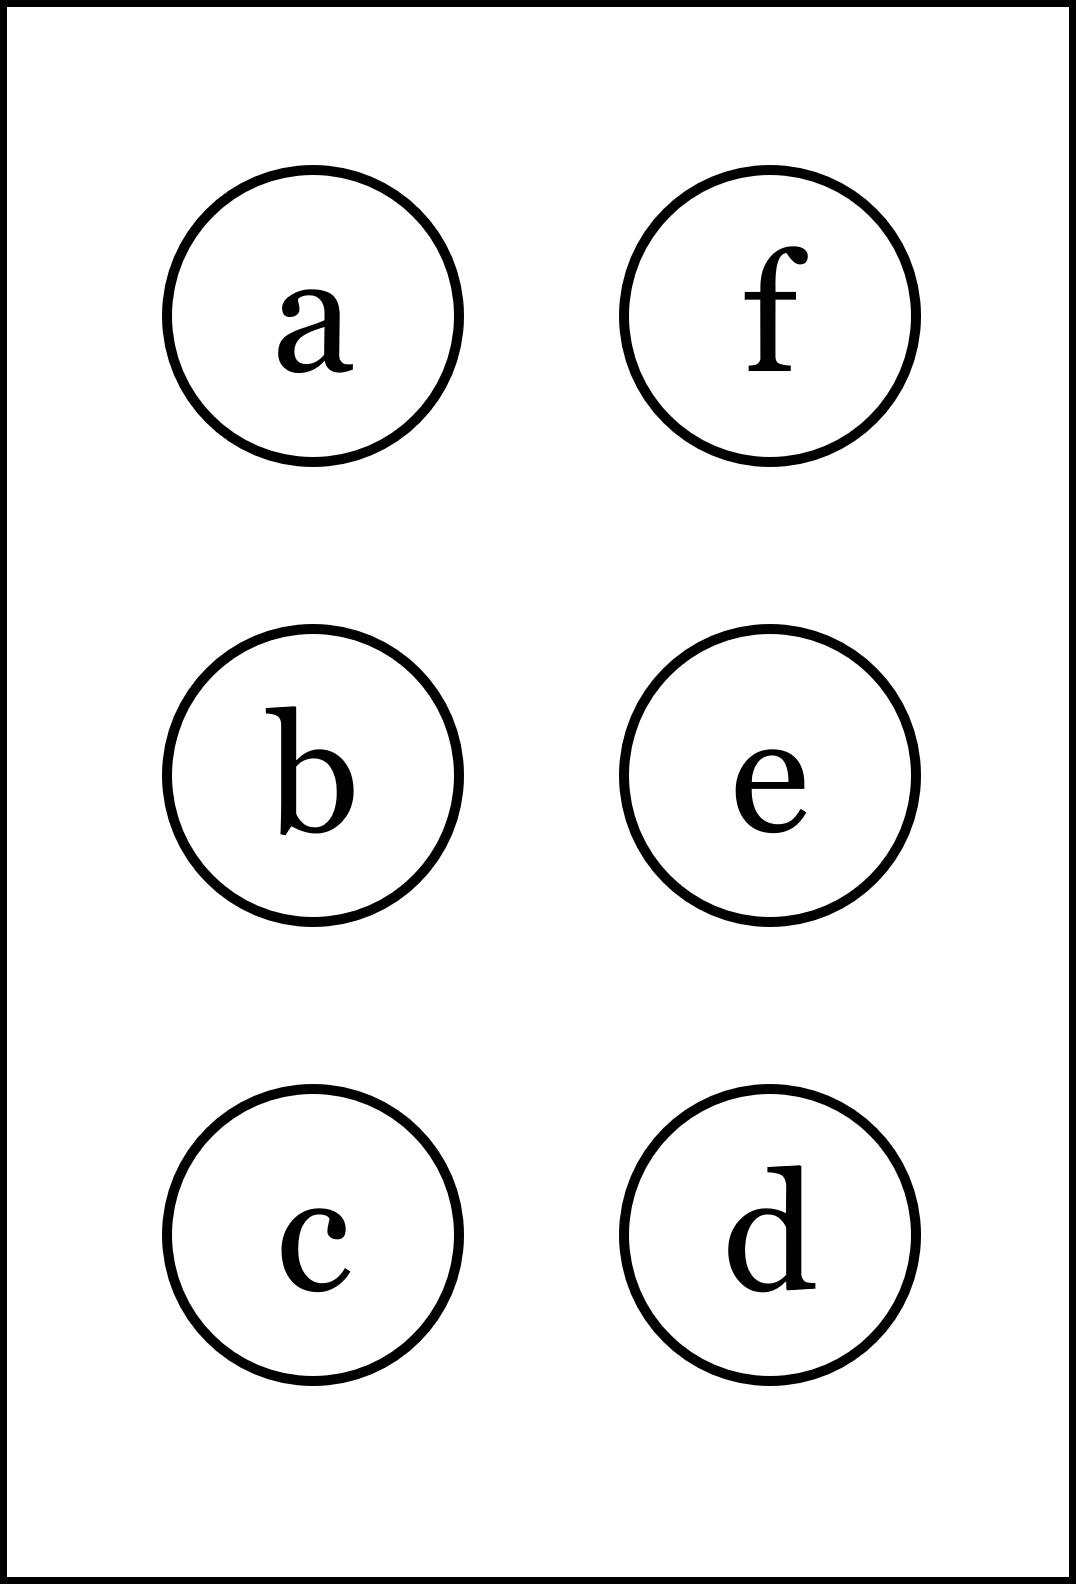
\includegraphics[height=40mm]{../images/braille.png}
{\small Písmeno Braillovej abecedy}
\end{center}
\end{minipage}
\end{center}
\end{minipage}
&
\begin{minipage}[c][104.5mm][t]{0.5\linewidth}
\begin{center}
\vspace{7mm}
{\huge Derivácie, skupina \textit{Iota $\iota$} -\romannumeral2}\\[5mm]
\textit{Meno:}\phantom{xxxxxxxxxxxxxxxxxxxxxxxxxxxxxxxxxxxxxxxxxxxxxxxxxxxxxxxxxxxxxxxxx}\\[5mm]
\begin{minipage}{0.95\linewidth}
\begin{center}
\textbf{Vypočítej derivace.} Pokud se výsledky shodují s těmi za otazníky,\\tak napravo obarvi příslušející kroužek načerno. \textbf{Spolu odevzdejte výsledné slovo}.
\end{center}
\end{minipage}
\\[1mm]
\begin{minipage}{0.79\linewidth}
\begin{center}
\begin{varwidth}{\linewidth}
\begin{enumerate}
\normalsize
\item $-3x^4+5x^3+9x^2+8x+6$\quad \dotfill\; ???\;\dotfill \quad $-12x^3+15x^2+18x+8$
\item $\cfrac{2x^2-2x+4}{-5x+2}$\quad \dotfill\; ???\;\dotfill \quad $\cfrac{-10x^2-8x+16}{25x^2-20x+4}$
\item $\frac{4}{x}\sqrt{-x+3}$\quad \dotfill\; ???\;\dotfill \quad $\frac{4x-24}{x^2 \sqrt{\smash[b]{-x+3}}}$
\item $e^{-x^2+4x-6}$\quad \dotfill\; ???\;\dotfill \quad $e^{-x^2+4x-6}$
\item $\ln{\left(\frac{-3x+5}{-6x+4}\right)}$\quad \dotfill\; ???\;\dotfill \quad $\frac{-3}{-3x+5}+\frac{-6}{-6x+4}$
\item $\frac{e^{-3x+1}}{9x-8}$\quad \dotfill\; ???\;\dotfill \quad $\frac{+27x+15}{(9x-8)^2}e^{-3x+1}$
\end{enumerate}
\end{varwidth}
\end{center}
\end{minipage}
\begin{minipage}{0.20\linewidth}
\begin{center}
{\Huge\bfseries 2.} \\[2mm]
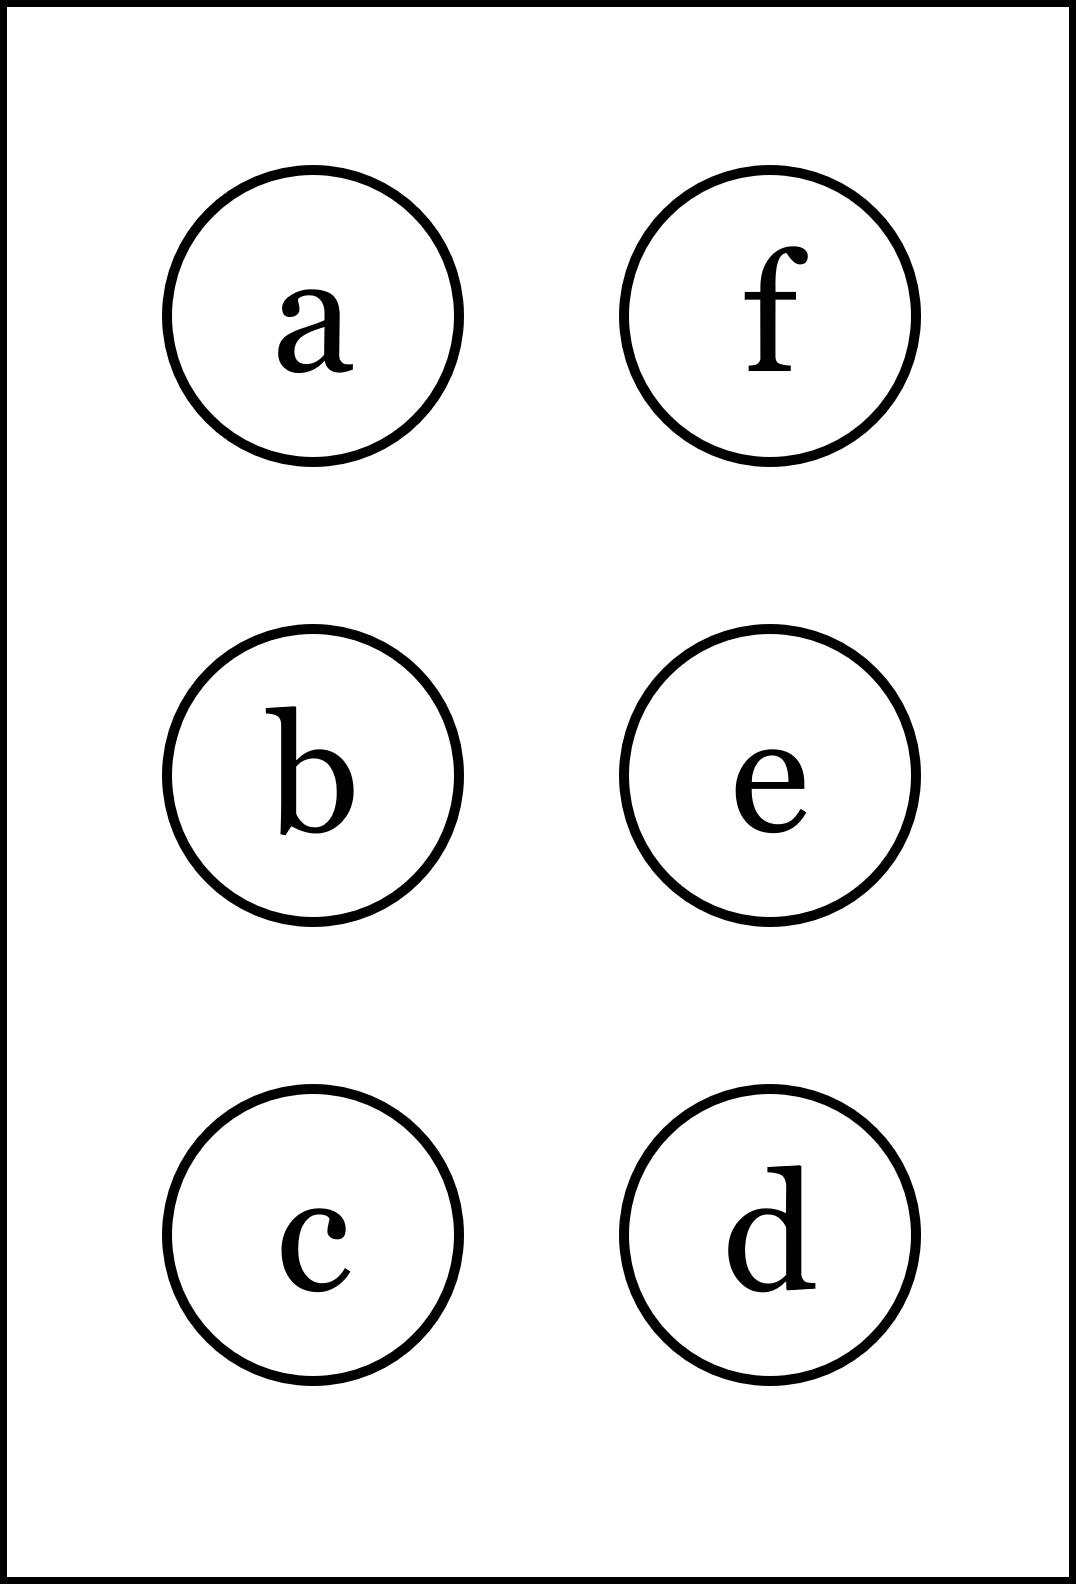
\includegraphics[height=40mm]{../images/braille.png}
{\small Písmeno Braillovej abecedy}
\end{center}
\end{minipage}
\end{center}
\end{minipage}
\\ \hdashline
\begin{minipage}[c][104.5mm][t]{0.5\linewidth}
\begin{center}
\vspace{7mm}
{\huge Derivácie, skupina \textit{Iota $\iota$} -\romannumeral3}\\[5mm]
\textit{Meno:}\phantom{xxxxxxxxxxxxxxxxxxxxxxxxxxxxxxxxxxxxxxxxxxxxxxxxxxxxxxxxxxxxxxxxx}\\[5mm]
\begin{minipage}{0.95\linewidth}
\begin{center}
\textbf{Vypočítej derivace.} Pokud se výsledky shodují s těmi za otazníky,\\tak napravo obarvi příslušející kroužek načerno. \textbf{Spolu odevzdejte výsledné slovo}.
\end{center}
\end{minipage}
\\[1mm]
\begin{minipage}{0.79\linewidth}
\begin{center}
\begin{varwidth}{\linewidth}
\begin{enumerate}
\normalsize
\item $8x^4-3x^3+x^2+2x+5$\quad \dotfill\; ???\;\dotfill \quad $32x^3-9x^2+2x+2$
\item $\cfrac{2x^2-4x-3}{x+2}$\quad \dotfill\; ???\;\dotfill \quad $\cfrac{2x^2-8x-5}{x^2+4x+4}$
\item $\frac{1}{x}\sqrt{4x-7}$\quad \dotfill\; ???\;\dotfill \quad $\frac{-4x+14}{2x^2 \sqrt{\smash[b]{4x-7}}}$
\item $e^{-8x^2-4x-3}$\quad \dotfill\; ???\;\dotfill \quad $e^{-8x^2-4x-3}$
\item $\ln{\left(\frac{-2x+1}{2x-2}\right)}$\quad \dotfill\; ???\;\dotfill \quad $\frac{-2}{-2x+1}-\frac{2}{2x-2}$
\item $\frac{e^{8x-7}}{-7x+2}$\quad \dotfill\; ???\;\dotfill \quad $\frac{-56x+23}{(-7x+2)^2}e^{8x-7}$
\end{enumerate}
\end{varwidth}
\end{center}
\end{minipage}
\begin{minipage}{0.20\linewidth}
\begin{center}
{\Huge\bfseries 3.} \\[2mm]
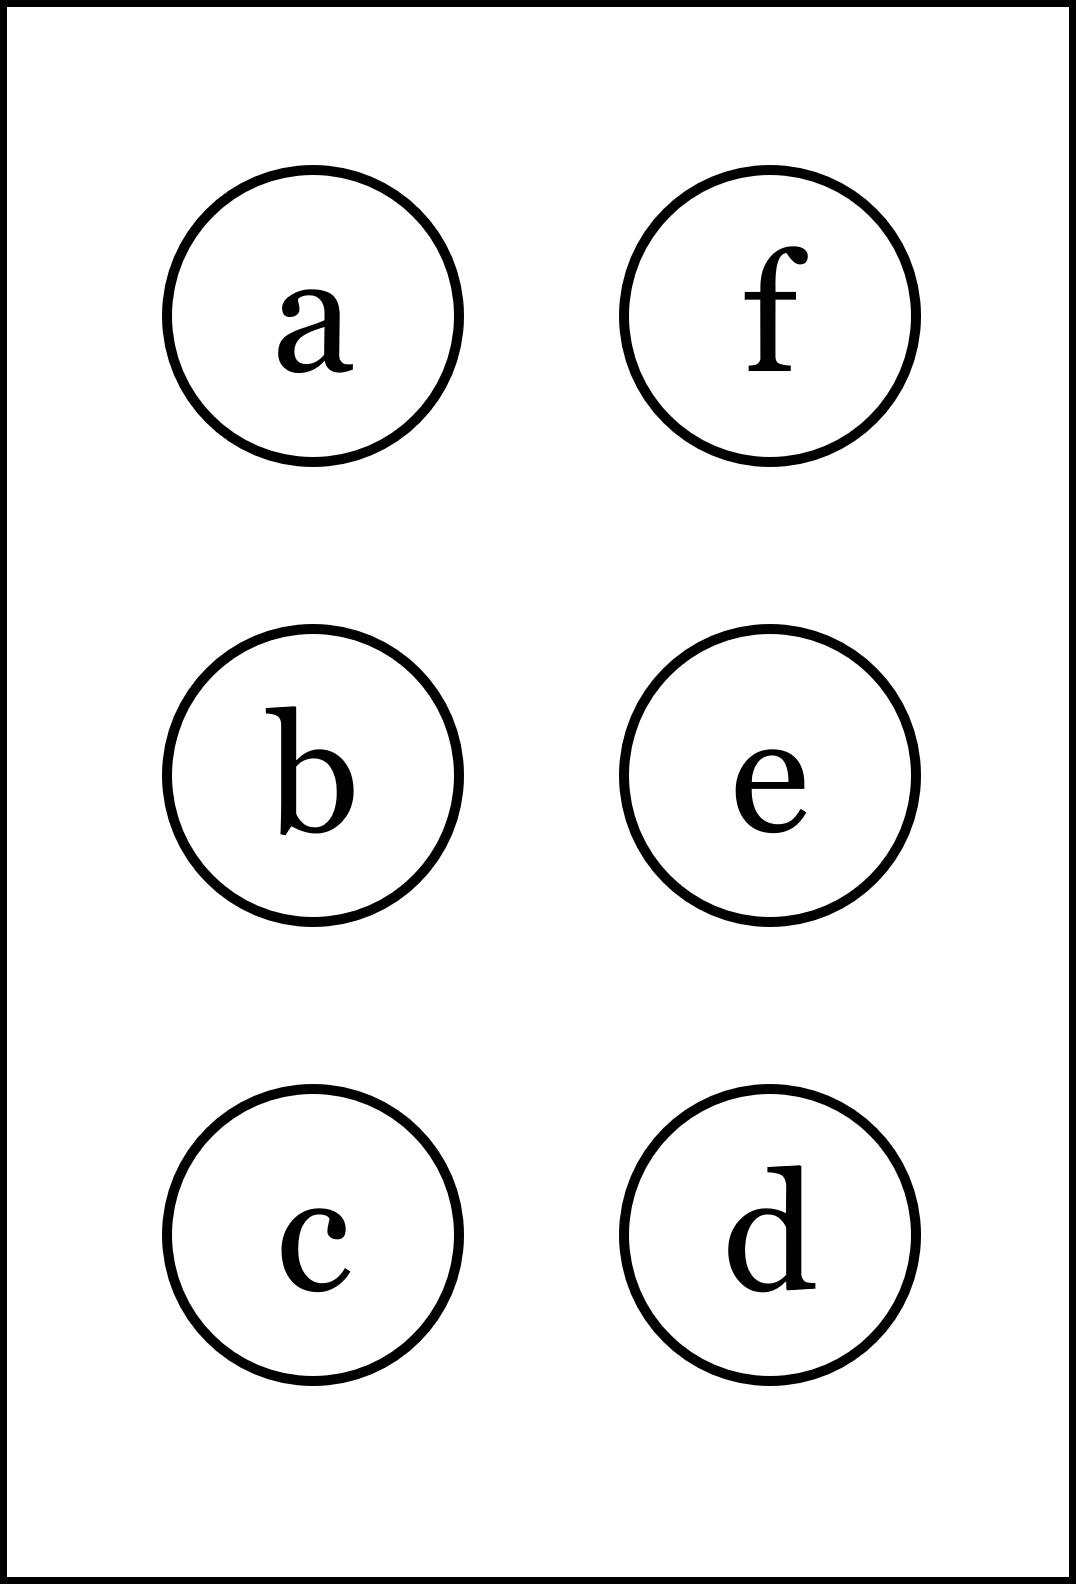
\includegraphics[height=40mm]{../images/braille.png}
{\small Písmeno Braillovej abecedy}
\end{center}
\end{minipage}
\end{center}
\end{minipage}
&
\begin{minipage}[c][104.5mm][t]{0.5\linewidth}
\begin{center}
\vspace{7mm}
{\huge Derivácie, skupina \textit{Iota $\iota$} -\romannumeral4}\\[5mm]
\textit{Meno:}\phantom{xxxxxxxxxxxxxxxxxxxxxxxxxxxxxxxxxxxxxxxxxxxxxxxxxxxxxxxxxxxxxxxxx}\\[5mm]
\begin{minipage}{0.95\linewidth}
\begin{center}
\textbf{Vypočítej derivace.} Pokud se výsledky shodují s těmi za otazníky,\\tak napravo obarvi příslušející kroužek načerno. \textbf{Spolu odevzdejte výsledné slovo}.
\end{center}
\end{minipage}
\\[1mm]
\begin{minipage}{0.79\linewidth}
\begin{center}
\begin{varwidth}{\linewidth}
\begin{enumerate}
\normalsize
\item $3x^4-x^3+5x^2+4x+2$\quad \dotfill\; ???\;\dotfill \quad $12x^3-3x^2+10x+4$
\item $\cfrac{-3x^2-6x-2}{-2x-2}$\quad \dotfill\; ???\;\dotfill \quad $\cfrac{6x^2-12x+8}{4x^2+8x+4}$
\item $\frac{-9}{x}\sqrt{-2x+2}$\quad \dotfill\; ???\;\dotfill \quad $\frac{-18x+36}{2x^2 \sqrt{\smash[b]{-2x+2}}}$
\item $e^{-9x^2+3x-4}$\quad \dotfill\; ???\;\dotfill \quad $e^{-9x^2+3x-4}$
\item $\ln{\left(\frac{6x-4}{-5x-2}\right)}$\quad \dotfill\; ???\;\dotfill \quad $\frac{6}{6x-4}-\frac{-5}{-5x-2}$
\item $\frac{e^{x-6}}{x+7}$\quad \dotfill\; ???\;\dotfill \quad $\frac{-x+6}{(x+7)^2}e^{x-6}$
\end{enumerate}
\end{varwidth}
\end{center}
\end{minipage}
\begin{minipage}{0.20\linewidth}
\begin{center}
{\Huge\bfseries 4.} \\[2mm]
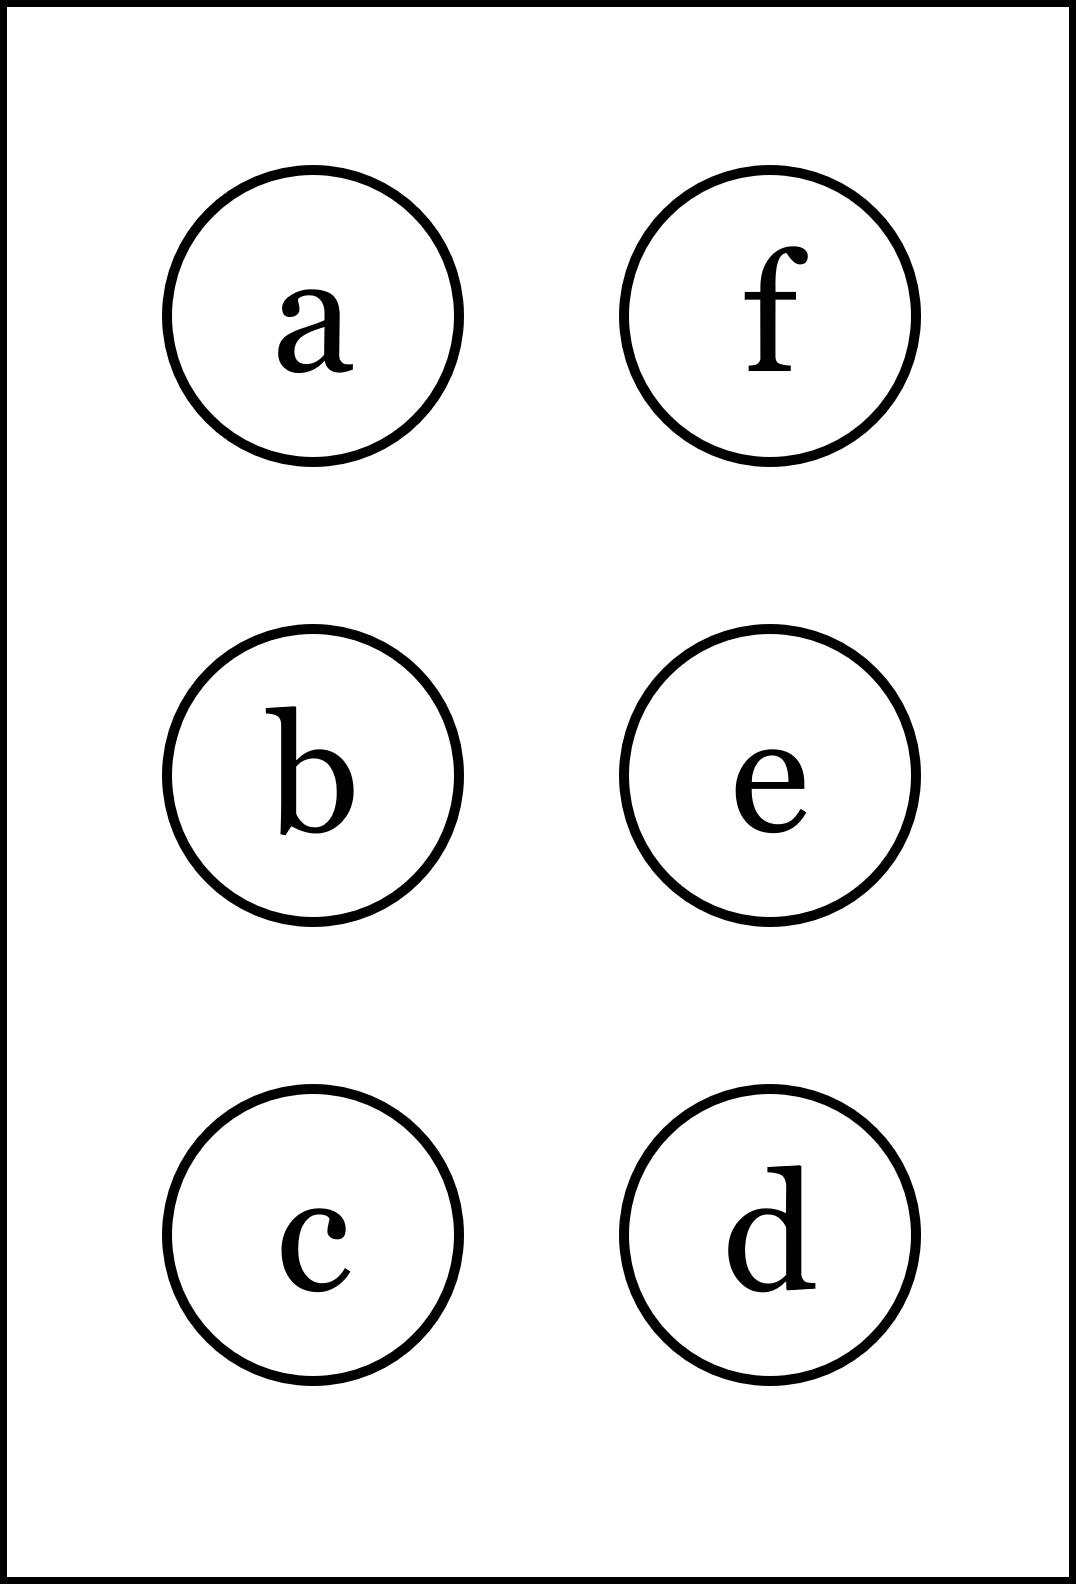
\includegraphics[height=40mm]{../images/braille.png}
{\small Písmeno Braillovej abecedy}
\end{center}
\end{minipage}
\end{center}
\end{minipage}
%
\end{tabular}
\newpage
\thispagestyle{empty}
\begin{tabular}{c:c}
\begin{minipage}[c][104.5mm][t]{0.5\linewidth}
\begin{center}
\vspace{7mm}
{\huge Derivácie, skupina \textit{Kappa $\kappa$} -\romannumeral1}\\[5mm]
\textit{Meno:}\phantom{xxxxxxxxxxxxxxxxxxxxxxxxxxxxxxxxxxxxxxxxxxxxxxxxxxxxxxxxxxxxxxxxx}\\[5mm]
\begin{minipage}{0.95\linewidth}
\begin{center}
\textbf{Vypočítej derivace.} Pokud se výsledky shodují s těmi za otazníky,\\tak napravo obarvi příslušející kroužek načerno. \textbf{Spolu odevzdejte výsledné slovo}.
\end{center}
\end{minipage}
\\[1mm]
\begin{minipage}{0.79\linewidth}
\begin{center}
\begin{varwidth}{\linewidth}
\begin{enumerate}
\normalsize
\item $-7x^4+3x^3-2x^2-4x-2$\quad \dotfill\; ???\;\dotfill \quad $-7x^3+3x^2-2x-4$
\item $\cfrac{-x^2+3x+2}{2x+1}$\quad \dotfill\; ???\;\dotfill \quad $\cfrac{-2x^2-2x-1}{4x^2+4x+1}$
\item $\frac{-1}{x}\sqrt{-2x-2}$\quad \dotfill\; ???\;\dotfill \quad $\frac{-2x-4}{x^2 \sqrt{\smash[b]{-2x-2}}}$
\item $e^{4x^2+3x-2}$\quad \dotfill\; ???\;\dotfill \quad $e^{4x^2+3x-2}$
\item $\ln{\left(\frac{-2x+1}{5x+5}\right)}$\quad \dotfill\; ???\;\dotfill \quad $\frac{-2}{-2x+1}-\frac{5}{5x+5}$
\item $\frac{e^{x+5}}{-x-2}$\quad \dotfill\; ???\;\dotfill \quad $\frac{-x-1}{(-x-2)^2}e^{x+5}$
\end{enumerate}
\end{varwidth}
\end{center}
\end{minipage}
\begin{minipage}{0.20\linewidth}
\begin{center}
{\Huge\bfseries 1.} \\[2mm]
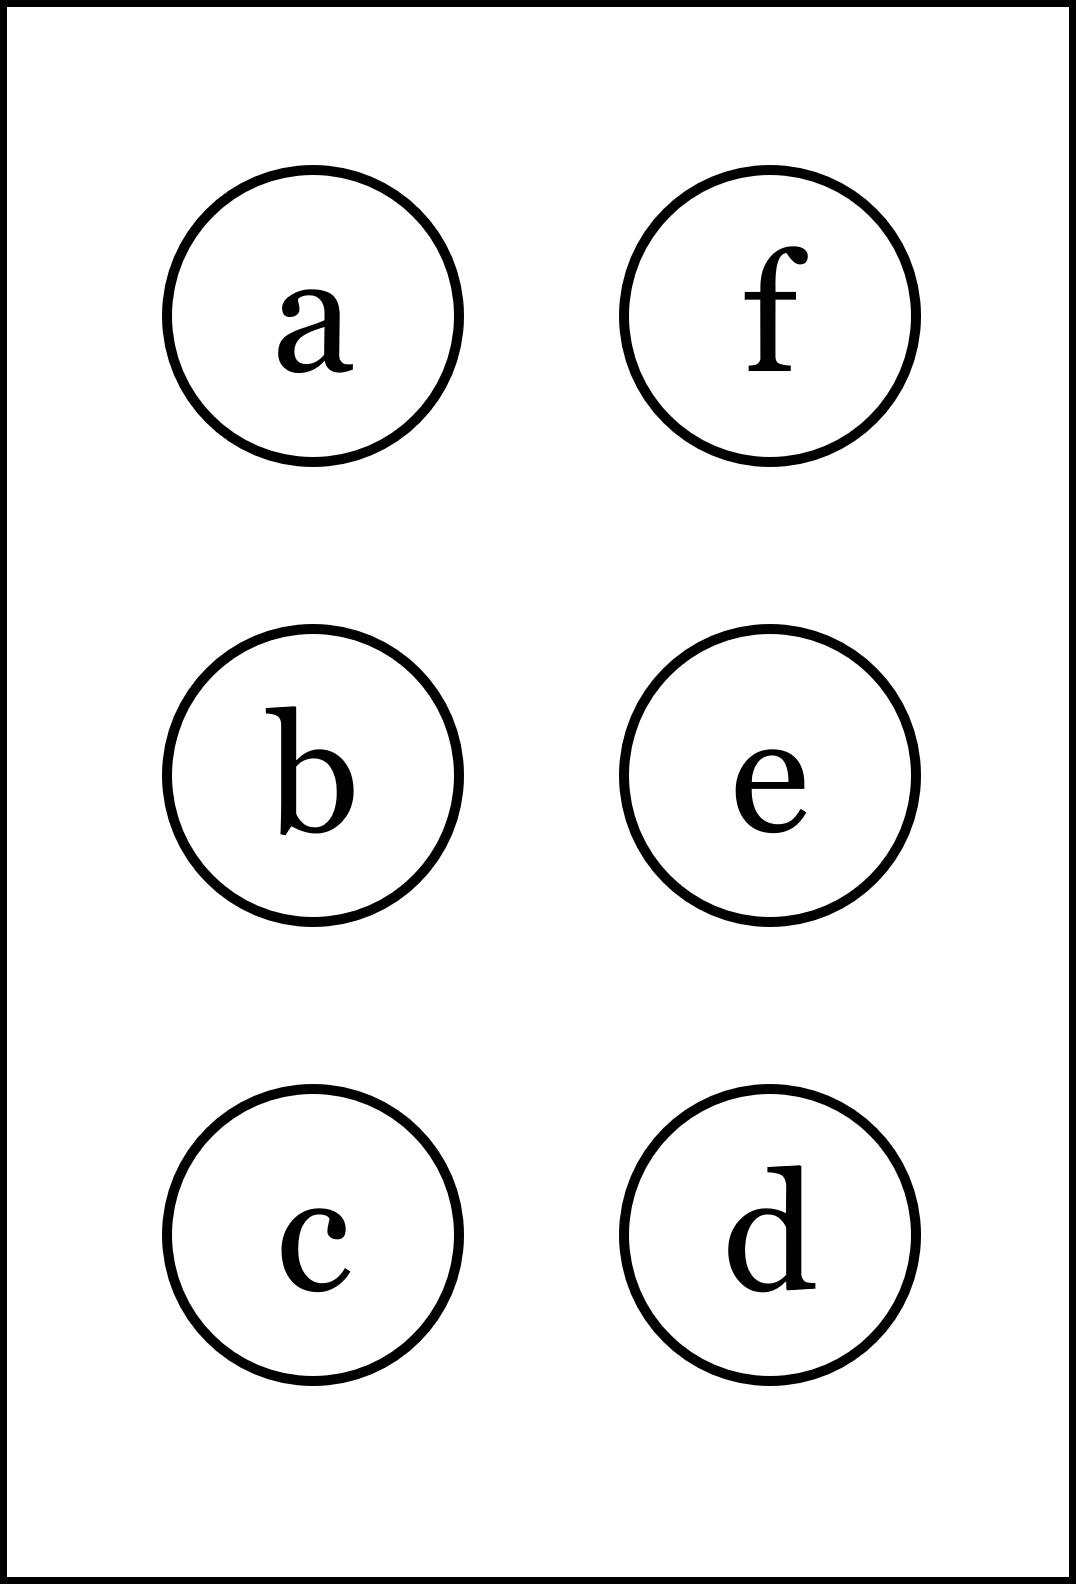
\includegraphics[height=40mm]{../images/braille.png}
{\small Písmeno Braillovej abecedy}
\end{center}
\end{minipage}
\end{center}
\end{minipage}
&
\begin{minipage}[c][104.5mm][t]{0.5\linewidth}
\begin{center}
\vspace{7mm}
{\huge Derivácie, skupina \textit{Kappa $\kappa$} -\romannumeral2}\\[5mm]
\textit{Meno:}\phantom{xxxxxxxxxxxxxxxxxxxxxxxxxxxxxxxxxxxxxxxxxxxxxxxxxxxxxxxxxxxxxxxxx}\\[5mm]
\begin{minipage}{0.95\linewidth}
\begin{center}
\textbf{Vypočítej derivace.} Pokud se výsledky shodují s těmi za otazníky,\\tak napravo obarvi příslušející kroužek načerno. \textbf{Spolu odevzdejte výsledné slovo}.
\end{center}
\end{minipage}
\\[1mm]
\begin{minipage}{0.79\linewidth}
\begin{center}
\begin{varwidth}{\linewidth}
\begin{enumerate}
\normalsize
\item $3x^4+x^3-2x^2-3x+1$\quad \dotfill\; ???\;\dotfill \quad $12x^3+3x^2-4x-3$
\item $\cfrac{-x^2-4x-1}{4x-2}$\quad \dotfill\; ???\;\dotfill \quad $\cfrac{-4x^2-4x+12}{16x^2-16x+4}$
\item $\frac{-3}{x}\sqrt{-5x+1}$\quad \dotfill\; ???\;\dotfill \quad $\frac{-15x+6}{x^2 \sqrt{\smash[b]{-5x+1}}}$
\item $e^{-2x^2-4x-2}$\quad \dotfill\; ???\;\dotfill \quad $(-4x-4)e^{-2x^2-4x-2}$
\item $\ln{\left(\frac{-x-1}{6x+5}\right)}$\quad \dotfill\; ???\;\dotfill \quad $\frac{-1}{-x-1}+\frac{6}{6x+5}$
\item $\frac{e^{7x+7}}{-x+9}$\quad \dotfill\; ???\;\dotfill \quad $\frac{+7x+64}{(-x+9)^2}e^{7x+7}$
\end{enumerate}
\end{varwidth}
\end{center}
\end{minipage}
\begin{minipage}{0.20\linewidth}
\begin{center}
{\Huge\bfseries 2.} \\[2mm]
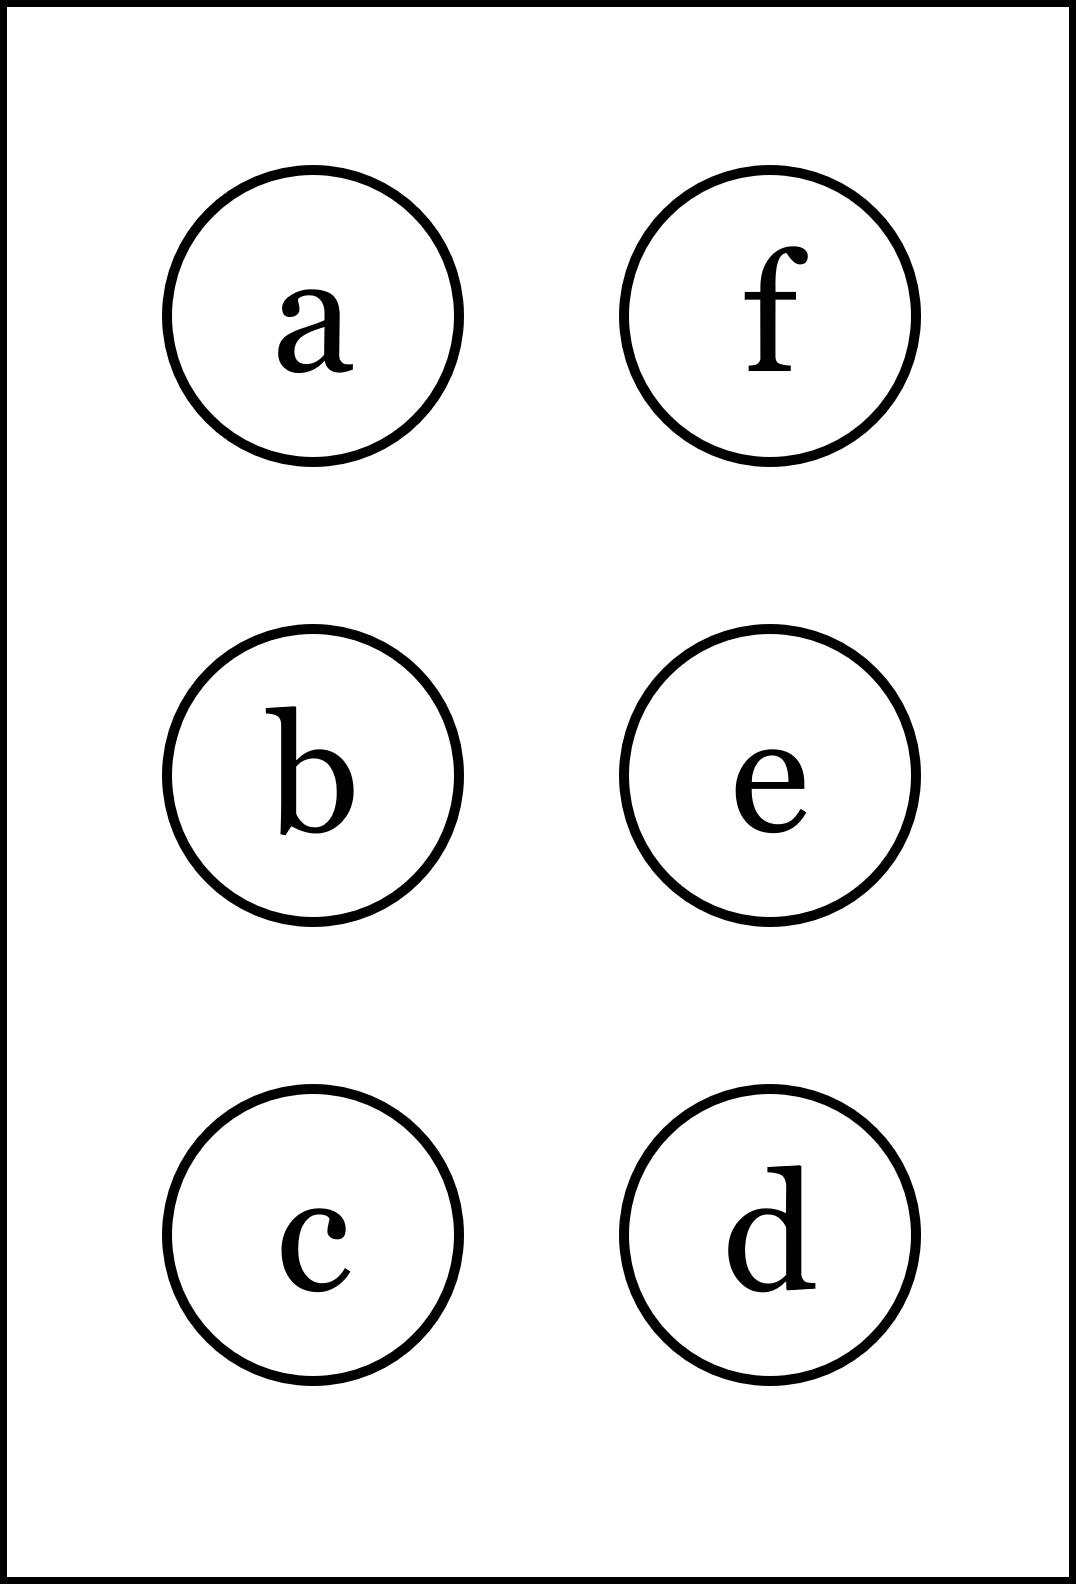
\includegraphics[height=40mm]{../images/braille.png}
{\small Písmeno Braillovej abecedy}
\end{center}
\end{minipage}
\end{center}
\end{minipage}
\\ \hdashline
\begin{minipage}[c][104.5mm][t]{0.5\linewidth}
\begin{center}
\vspace{7mm}
{\huge Derivácie, skupina \textit{Kappa $\kappa$} -\romannumeral3}\\[5mm]
\textit{Meno:}\phantom{xxxxxxxxxxxxxxxxxxxxxxxxxxxxxxxxxxxxxxxxxxxxxxxxxxxxxxxxxxxxxxxxx}\\[5mm]
\begin{minipage}{0.95\linewidth}
\begin{center}
\textbf{Vypočítej derivace.} Pokud se výsledky shodují s těmi za otazníky,\\tak napravo obarvi příslušející kroužek načerno. \textbf{Spolu odevzdejte výsledné slovo}.
\end{center}
\end{minipage}
\\[1mm]
\begin{minipage}{0.79\linewidth}
\begin{center}
\begin{varwidth}{\linewidth}
\begin{enumerate}
\normalsize
\item $3x^4-2x^3+2x^2+3x+3$\quad \dotfill\; ???\;\dotfill \quad $12x^3-6x^2+4x+3$
\item $\cfrac{-4x^2+5x+3}{-2x+2}$\quad \dotfill\; ???\;\dotfill \quad $\cfrac{8x^2+16x+16}{4x^2-8x+4}$
\item $\frac{8}{x}\sqrt{-6x-4}$\quad \dotfill\; ???\;\dotfill \quad $\frac{48x+64}{2x^2 \sqrt{\smash[b]{-6x-4}}}$
\item $e^{3x^2+4x+5}$\quad \dotfill\; ???\;\dotfill \quad $e^{3x^2+4x+5}$
\item $\ln{\left(\frac{2x-2}{x+1}\right)}$\quad \dotfill\; ???\;\dotfill \quad $\frac{2}{2x-2}+\frac{1}{x+1}$
\item $\frac{e^{4x+3}}{-3x+2}$\quad \dotfill\; ???\;\dotfill \quad $\frac{-12x+11}{(-3x+2)^2}e^{4x+3}$
\end{enumerate}
\end{varwidth}
\end{center}
\end{minipage}
\begin{minipage}{0.20\linewidth}
\begin{center}
{\Huge\bfseries 3.} \\[2mm]
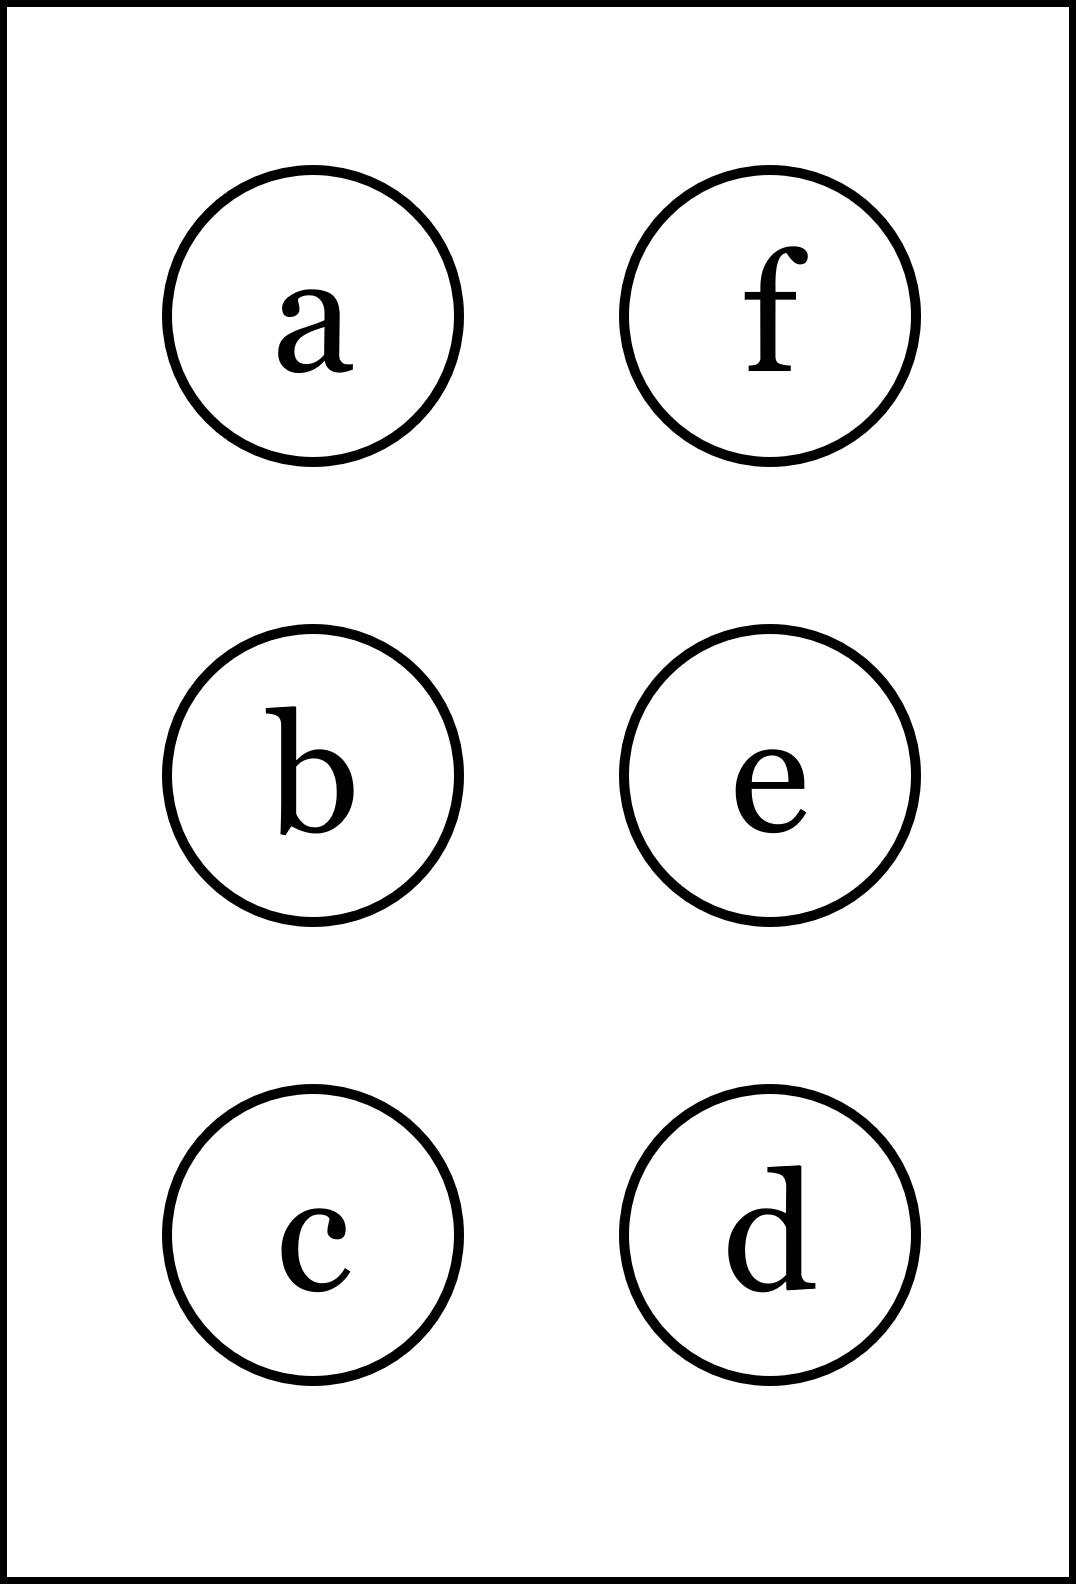
\includegraphics[height=40mm]{../images/braille.png}
{\small Písmeno Braillovej abecedy}
\end{center}
\end{minipage}
\end{center}
\end{minipage}
&
\begin{minipage}[c][104.5mm][t]{0.5\linewidth}
\begin{center}
\vspace{7mm}
{\huge Derivácie, skupina \textit{Kappa $\kappa$} -\romannumeral4}\\[5mm]
\textit{Meno:}\phantom{xxxxxxxxxxxxxxxxxxxxxxxxxxxxxxxxxxxxxxxxxxxxxxxxxxxxxxxxxxxxxxxxx}\\[5mm]
\begin{minipage}{0.95\linewidth}
\begin{center}
\textbf{Vypočítej derivace.} Pokud se výsledky shodují s těmi za otazníky,\\tak napravo obarvi příslušející kroužek načerno. \textbf{Spolu odevzdejte výsledné slovo}.
\end{center}
\end{minipage}
\\[1mm]
\begin{minipage}{0.79\linewidth}
\begin{center}
\begin{varwidth}{\linewidth}
\begin{enumerate}
\normalsize
\item $-x^4+8x^3-4x^2-6x+4$\quad \dotfill\; ???\;\dotfill \quad $-4x^3+24x^2-8x-6$
\item $\cfrac{-x^2+4x-1}{x-5}$\quad \dotfill\; ???\;\dotfill \quad $\cfrac{-x^2-10x-19}{x^2-10x+25}$
\item $\frac{-2}{x}\sqrt{-7x-9}$\quad \dotfill\; ???\;\dotfill \quad $\frac{-14x-36}{x^2 \sqrt{\smash[b]{-7x-9}}}$
\item $e^{2x^2-3x+8}$\quad \dotfill\; ???\;\dotfill \quad $e^{2x^2-3x+8}$
\item $\ln{\left(\frac{2x+4}{-2x-8}\right)}$\quad \dotfill\; ???\;\dotfill \quad $\frac{2}{2x+4}+\frac{-2}{-2x-8}$
\item $\frac{e^{-3x+3}}{-x+4}$\quad \dotfill\; ???\;\dotfill \quad $\frac{-3x-11}{(-x+4)^2}e^{-3x+3}$
\end{enumerate}
\end{varwidth}
\end{center}
\end{minipage}
\begin{minipage}{0.20\linewidth}
\begin{center}
{\Huge\bfseries 4.} \\[2mm]
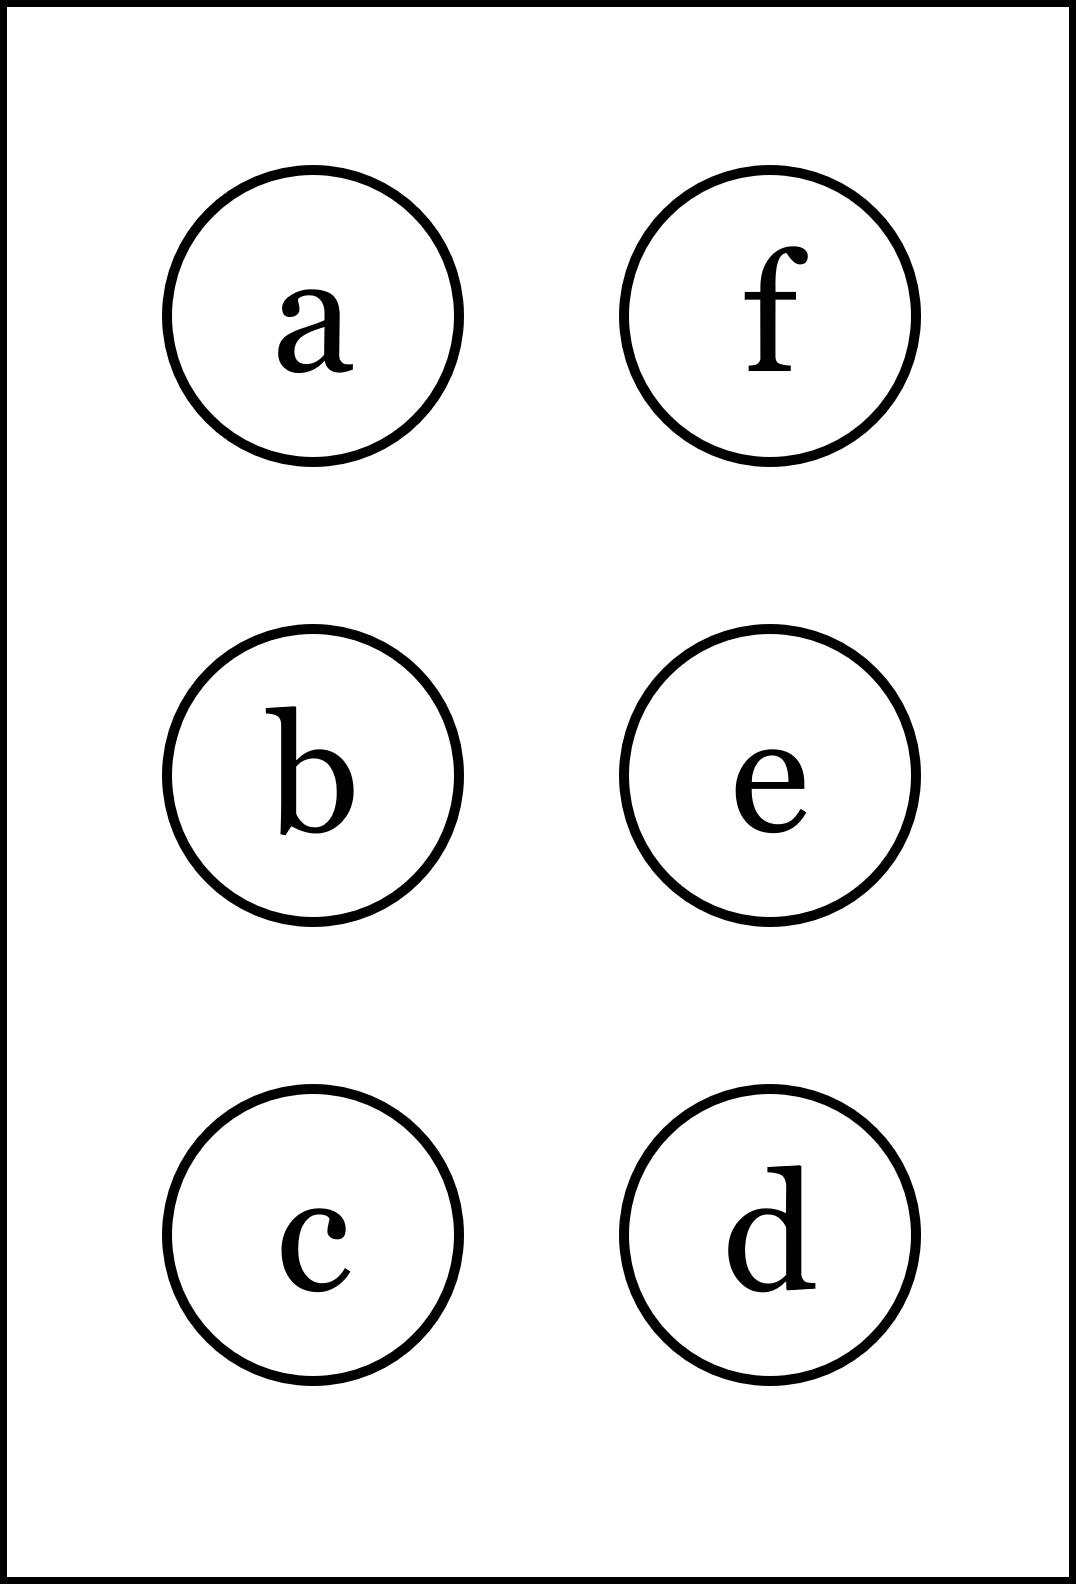
\includegraphics[height=40mm]{../images/braille.png}
{\small Písmeno Braillovej abecedy}
\end{center}
\end{minipage}
\end{center}
\end{minipage}
%
\end{tabular}
\newpage
\thispagestyle{empty}
\begin{tabular}{c:c}
\begin{minipage}[c][104.5mm][t]{0.5\linewidth}
\begin{center}
\vspace{7mm}
{\huge Derivácie, skupina \textit{Lambda $\lambda$} -\romannumeral1}\\[5mm]
\textit{Meno:}\phantom{xxxxxxxxxxxxxxxxxxxxxxxxxxxxxxxxxxxxxxxxxxxxxxxxxxxxxxxxxxxxxxxxx}\\[5mm]
\begin{minipage}{0.95\linewidth}
\begin{center}
\textbf{Vypočítej derivace.} Pokud se výsledky shodují s těmi za otazníky,\\tak napravo obarvi příslušející kroužek načerno. \textbf{Spolu odevzdejte výsledné slovo}.
\end{center}
\end{minipage}
\\[1mm]
\begin{minipage}{0.79\linewidth}
\begin{center}
\begin{varwidth}{\linewidth}
\begin{enumerate}
\normalsize
\item $-5x^4-3x^3+8x^2-6x-5$\quad \dotfill\; ???\;\dotfill \quad $-20x^3-9x^2+16x-6$
\item $\cfrac{2x^2+3x-3}{-x-5}$\quad \dotfill\; ???\;\dotfill \quad $\cfrac{-2x^2-20x-18}{x^2+10x+25}$
\item $\frac{-2}{x}\sqrt{-2x-1}$\quad \dotfill\; ???\;\dotfill \quad $\frac{-4x-4}{2x^2 \sqrt{\smash[b]{-2x-1}}}$
\item $e^{-2x^2-4x-3}$\quad \dotfill\; ???\;\dotfill \quad $e^{-2x^2-4x-3}$
\item $\ln{\left(\frac{2x-1}{-4x+6}\right)}$\quad \dotfill\; ???\;\dotfill \quad $\frac{2}{2x-1}-\frac{-4}{-4x+6}$
\item $\frac{e^{-x-5}}{-2x+5}$\quad \dotfill\; ???\;\dotfill \quad $\frac{-2x-3}{(-2x+5)^2}e^{-x-5}$
\end{enumerate}
\end{varwidth}
\end{center}
\end{minipage}
\begin{minipage}{0.20\linewidth}
\begin{center}
{\Huge\bfseries 1.} \\[2mm]
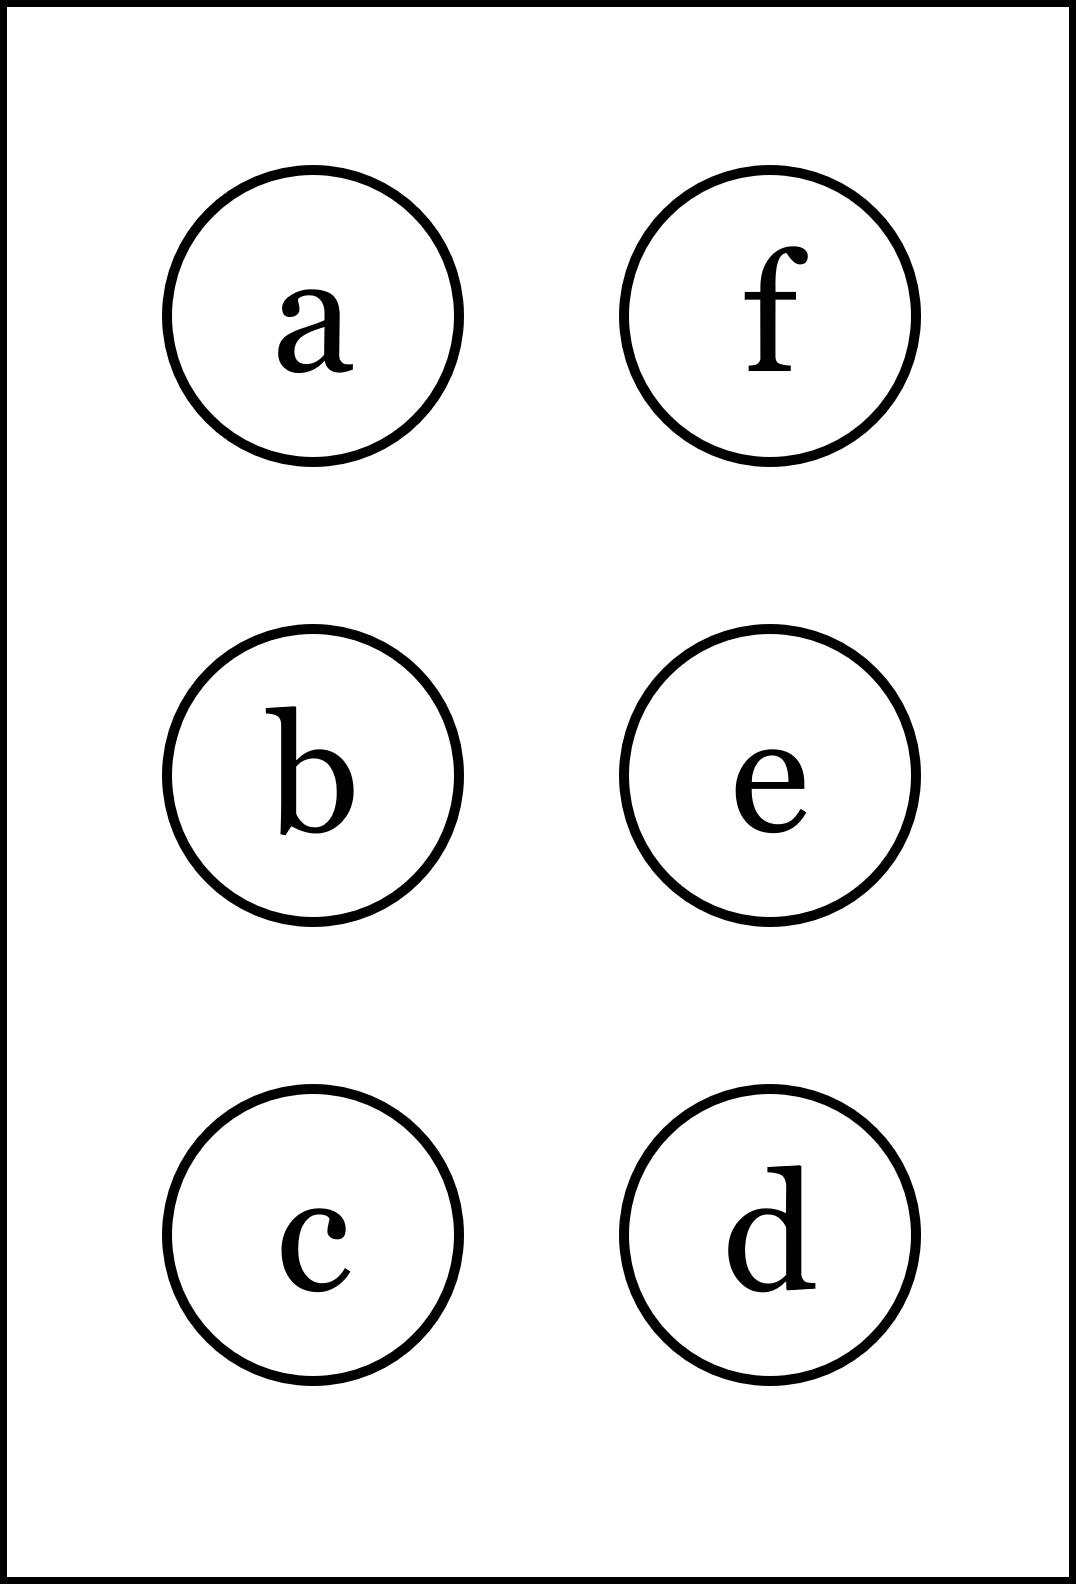
\includegraphics[height=40mm]{../images/braille.png}
{\small Písmeno Braillovej abecedy}
\end{center}
\end{minipage}
\end{center}
\end{minipage}
&
\begin{minipage}[c][104.5mm][t]{0.5\linewidth}
\begin{center}
\vspace{7mm}
{\huge Derivácie, skupina \textit{Lambda $\lambda$} -\romannumeral2}\\[5mm]
\textit{Meno:}\phantom{xxxxxxxxxxxxxxxxxxxxxxxxxxxxxxxxxxxxxxxxxxxxxxxxxxxxxxxxxxxxxxxxx}\\[5mm]
\begin{minipage}{0.95\linewidth}
\begin{center}
\textbf{Vypočítej derivace.} Pokud se výsledky shodují s těmi za otazníky,\\tak napravo obarvi příslušející kroužek načerno. \textbf{Spolu odevzdejte výsledné slovo}.
\end{center}
\end{minipage}
\\[1mm]
\begin{minipage}{0.79\linewidth}
\begin{center}
\begin{varwidth}{\linewidth}
\begin{enumerate}
\normalsize
\item $-x^4-6x^3+8x^2+x+5$\quad \dotfill\; ???\;\dotfill \quad $-4x^3-18x^2+16x+1$
\item $\cfrac{-2x^2+2x+6}{5x+2}$\quad \dotfill\; ???\;\dotfill \quad $\cfrac{-10x^2+8x-26}{25x^2+20x+4}$
\item $\frac{2}{x}\sqrt{-4x+1}$\quad \dotfill\; ???\;\dotfill \quad $\frac{8x-4}{x^2 \sqrt{\smash[b]{-4x+1}}}$
\item $e^{6x^2-5x+4}$\quad \dotfill\; ???\;\dotfill \quad $e^{6x^2-5x+4}$
\item $\ln{\left(\frac{-x-2}{9x+3}\right)}$\quad \dotfill\; ???\;\dotfill \quad $\frac{-1}{-x-2}+\frac{9}{9x+3}$
\item $\frac{e^{-5x+8}}{x+1}$\quad \dotfill\; ???\;\dotfill \quad $\frac{+5x-6}{(x+1)^2}e^{-5x+8}$
\end{enumerate}
\end{varwidth}
\end{center}
\end{minipage}
\begin{minipage}{0.20\linewidth}
\begin{center}
{\Huge\bfseries 2.} \\[2mm]
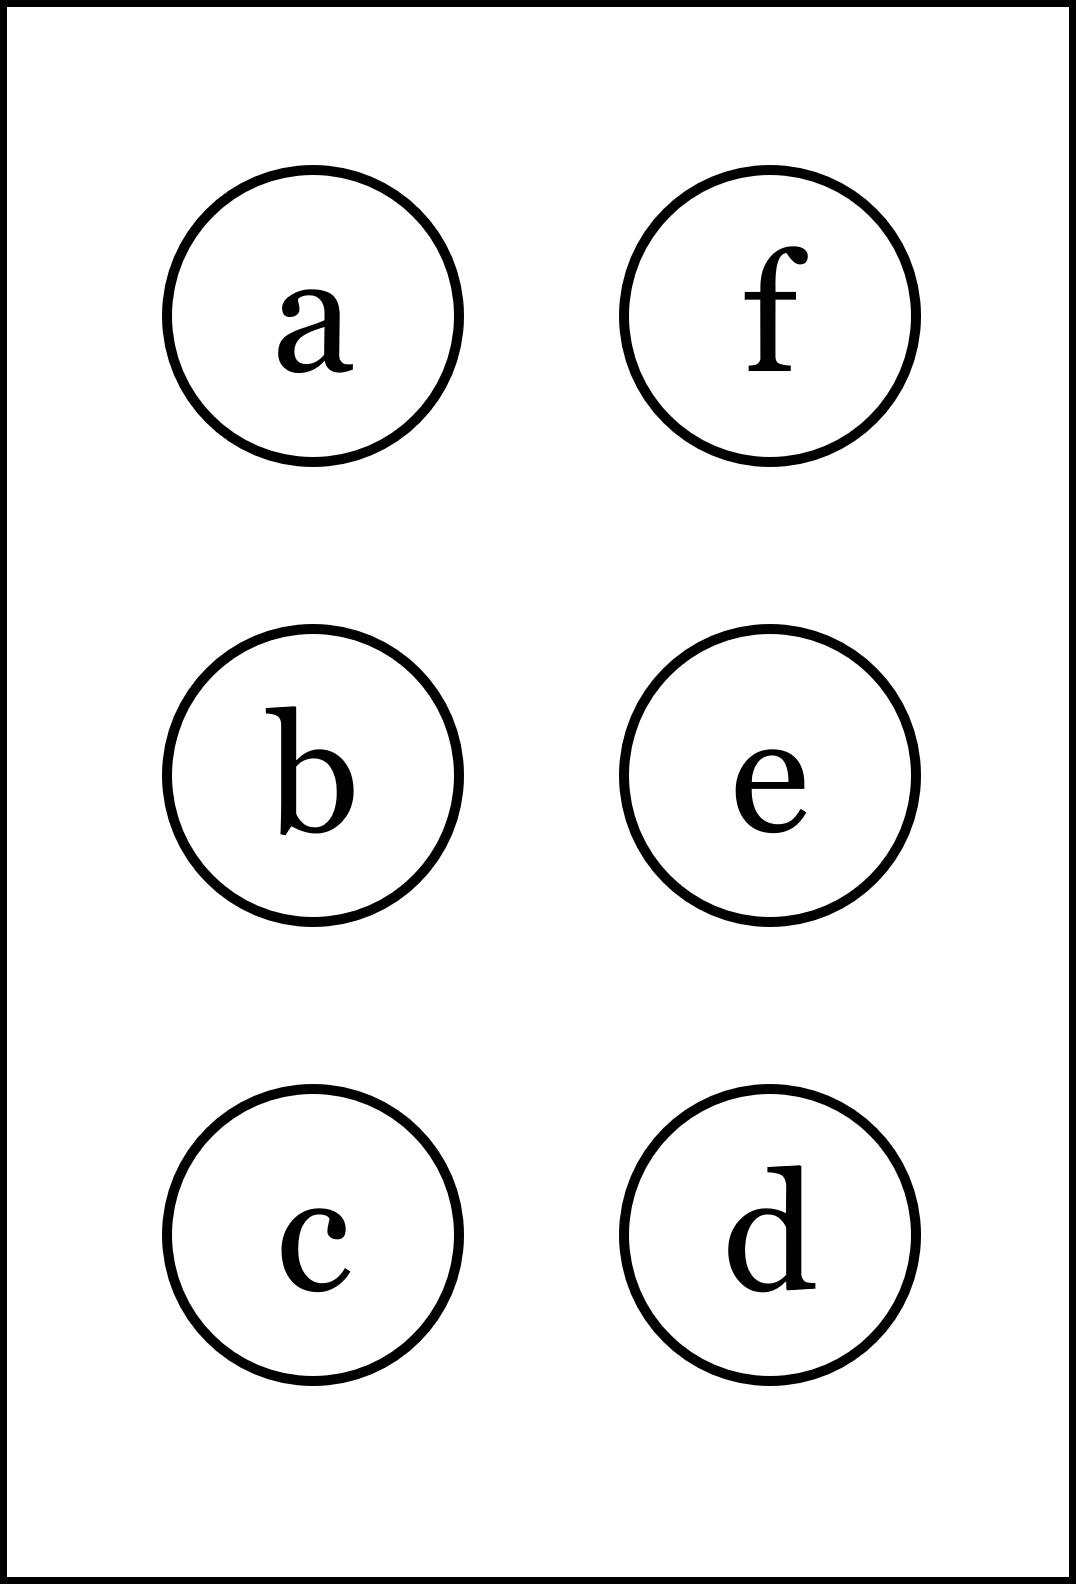
\includegraphics[height=40mm]{../images/braille.png}
{\small Písmeno Braillovej abecedy}
\end{center}
\end{minipage}
\end{center}
\end{minipage}
\\ \hdashline
\begin{minipage}[c][104.5mm][t]{0.5\linewidth}
\begin{center}
\vspace{7mm}
{\huge Derivácie, skupina \textit{Lambda $\lambda$} -\romannumeral3}\\[5mm]
\textit{Meno:}\phantom{xxxxxxxxxxxxxxxxxxxxxxxxxxxxxxxxxxxxxxxxxxxxxxxxxxxxxxxxxxxxxxxxx}\\[5mm]
\begin{minipage}{0.95\linewidth}
\begin{center}
\textbf{Vypočítej derivace.} Pokud se výsledky shodují s těmi za otazníky,\\tak napravo obarvi příslušející kroužek načerno. \textbf{Spolu odevzdejte výsledné slovo}.
\end{center}
\end{minipage}
\\[1mm]
\begin{minipage}{0.79\linewidth}
\begin{center}
\begin{varwidth}{\linewidth}
\begin{enumerate}
\normalsize
\item $-8x^4+5x^3+x^2+6x+1$\quad \dotfill\; ???\;\dotfill \quad $-32x^3+15x^2+2x+6$
\item $\cfrac{-5x^2+6x-2}{3x+1}$\quad \dotfill\; ???\;\dotfill \quad $\cfrac{-15x^2+10x+12}{9x^2+6x+1}$
\item $\frac{1}{x}\sqrt{-x+2}$\quad \dotfill\; ???\;\dotfill \quad $\frac{x-4}{x^2 \sqrt{\smash[b]{-x+2}}}$
\item $e^{2x^2-3x+1}$\quad \dotfill\; ???\;\dotfill \quad $e^{2x^2-3x+1}$
\item $\ln{\left(\frac{5x+2}{2x-5}\right)}$\quad \dotfill\; ???\;\dotfill \quad $\frac{5}{5x+2}-\frac{2}{2x-5}$
\item $\frac{e^{-7x-5}}{2x+3}$\quad \dotfill\; ???\;\dotfill \quad $\frac{-14x-23}{(2x+3)^2}e^{-7x-5}$
\end{enumerate}
\end{varwidth}
\end{center}
\end{minipage}
\begin{minipage}{0.20\linewidth}
\begin{center}
{\Huge\bfseries 3.} \\[2mm]
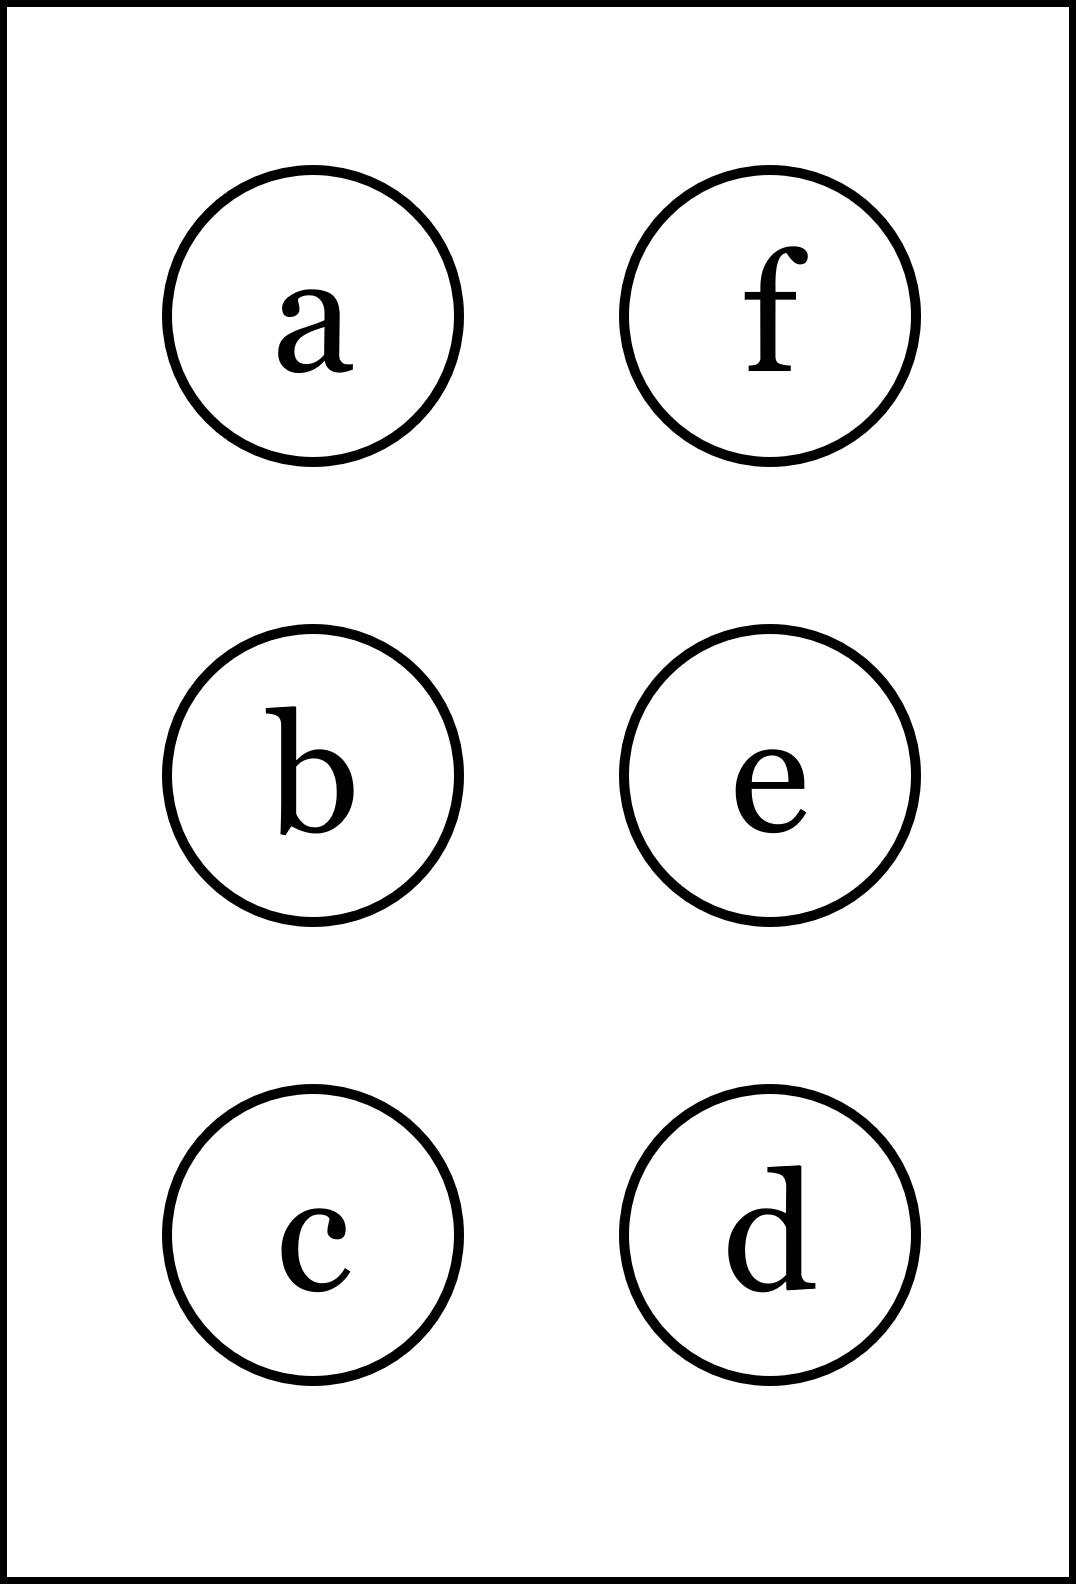
\includegraphics[height=40mm]{../images/braille.png}
{\small Písmeno Braillovej abecedy}
\end{center}
\end{minipage}
\end{center}
\end{minipage}
&
\begin{minipage}[c][104.5mm][t]{0.5\linewidth}
\begin{center}
\vspace{7mm}
{\huge Derivácie, skupina \textit{Lambda $\lambda$} -\romannumeral4}\\[5mm]
\textit{Meno:}\phantom{xxxxxxxxxxxxxxxxxxxxxxxxxxxxxxxxxxxxxxxxxxxxxxxxxxxxxxxxxxxxxxxxx}\\[5mm]
\begin{minipage}{0.95\linewidth}
\begin{center}
\textbf{Vypočítej derivace.} Pokud se výsledky shodují s těmi za otazníky,\\tak napravo obarvi příslušející kroužek načerno. \textbf{Spolu odevzdejte výsledné slovo}.
\end{center}
\end{minipage}
\\[1mm]
\begin{minipage}{0.79\linewidth}
\begin{center}
\begin{varwidth}{\linewidth}
\begin{enumerate}
\normalsize
\item $5x^4-3x^3+6x^2-6x+1$\quad \dotfill\; ???\;\dotfill \quad $20x^3-9x^2+12x-6$
\item $\cfrac{-x^2-x+5}{-4x+3}$\quad \dotfill\; ???\;\dotfill \quad $\cfrac{4x^2+6x+17}{16x^2-24x+9}$
\item $\frac{-9}{x}\sqrt{4x-7}$\quad \dotfill\; ???\;\dotfill \quad $\frac{36x-126}{x^2 \sqrt{\smash[b]{4x-7}}}$
\item $e^{-3x^2-2x-5}$\quad \dotfill\; ???\;\dotfill \quad $e^{-3x^2-2x-5}$
\item $\ln{\left(\frac{5x+9}{3x-1}\right)}$\quad \dotfill\; ???\;\dotfill \quad $\frac{5}{5x+9}+\frac{3}{3x-1}$
\item $\frac{e^{6x-6}}{-3x-5}$\quad \dotfill\; ???\;\dotfill \quad $\frac{+18x-27}{(-3x-5)^2}e^{6x-6}$
\end{enumerate}
\end{varwidth}
\end{center}
\end{minipage}
\begin{minipage}{0.20\linewidth}
\begin{center}
{\Huge\bfseries 4.} \\[2mm]
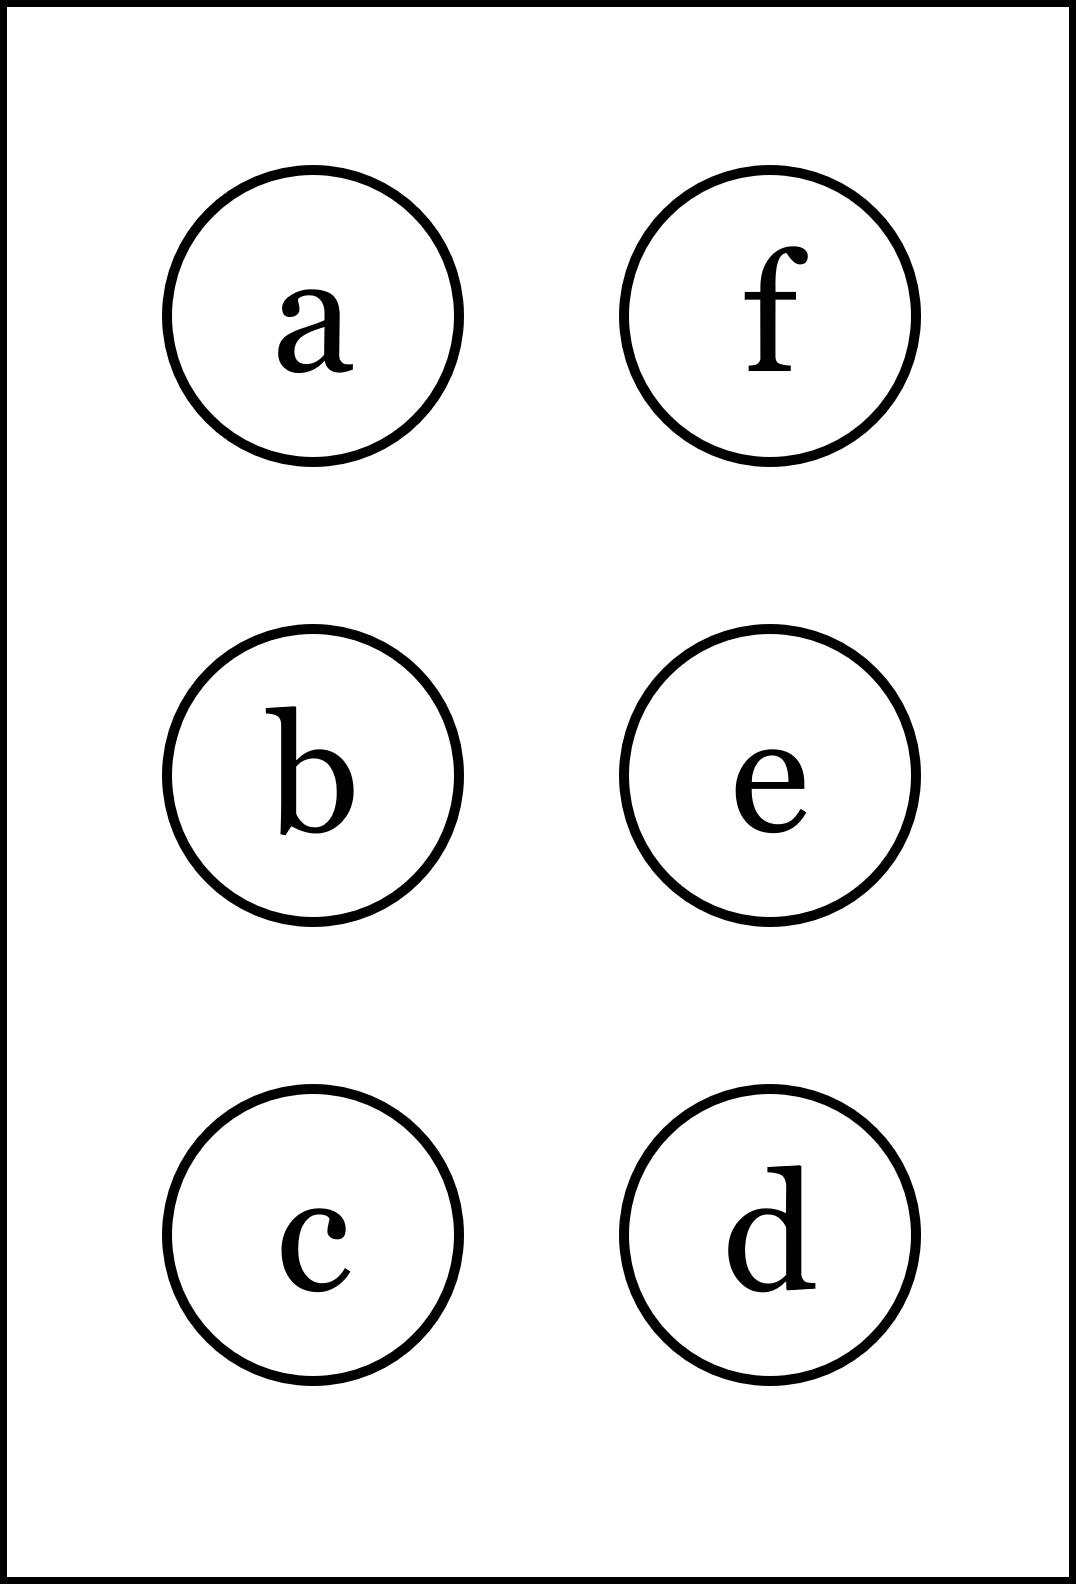
\includegraphics[height=40mm]{../images/braille.png}
{\small Písmeno Braillovej abecedy}
\end{center}
\end{minipage}
\end{center}
\end{minipage}
%
\end{tabular}
\newpage
\thispagestyle{empty}
\begin{tabular}{c:c}
\begin{minipage}[c][104.5mm][t]{0.5\linewidth}
\begin{center}
\vspace{7mm}
{\huge Derivácie, skupina \textit{Mu $\mu$} -\romannumeral1}\\[5mm]
\textit{Meno:}\phantom{xxxxxxxxxxxxxxxxxxxxxxxxxxxxxxxxxxxxxxxxxxxxxxxxxxxxxxxxxxxxxxxxx}\\[5mm]
\begin{minipage}{0.95\linewidth}
\begin{center}
\textbf{Vypočítej derivace.} Pokud se výsledky shodují s těmi za otazníky,\\tak napravo obarvi příslušející kroužek načerno. \textbf{Spolu odevzdejte výsledné slovo}.
\end{center}
\end{minipage}
\\[1mm]
\begin{minipage}{0.79\linewidth}
\begin{center}
\begin{varwidth}{\linewidth}
\begin{enumerate}
\normalsize
\item $-8x^4+8x^3-5x^2+8x+1$\quad \dotfill\; ???\;\dotfill \quad $-32x^3+24x^2-10x+8$
\item $\cfrac{2x^2+2x-1}{-2x+2}$\quad \dotfill\; ???\;\dotfill \quad $\cfrac{-4x^2+8x+2}{4x^2-8x+4}$
\item $\frac{2}{x}\sqrt{3x-8}$\quad \dotfill\; ???\;\dotfill \quad $\frac{-6x+32}{2x^2 \sqrt{\smash[b]{3x-8}}}$
\item $e^{-7x^2+2x-3}$\quad \dotfill\; ???\;\dotfill \quad $e^{-7x^2+2x-3}$
\item $\ln{\left(\frac{-2x+2}{-x-1}\right)}$\quad \dotfill\; ???\;\dotfill \quad $\frac{-2}{-2x+2}+\frac{-1}{-x-1}$
\item $\frac{e^{-5x+4}}{8x-2}$\quad \dotfill\; ???\;\dotfill \quad $\frac{-40x+2}{(8x-2)^2}e^{-5x+4}$
\end{enumerate}
\end{varwidth}
\end{center}
\end{minipage}
\begin{minipage}{0.20\linewidth}
\begin{center}
{\Huge\bfseries 1.} \\[2mm]
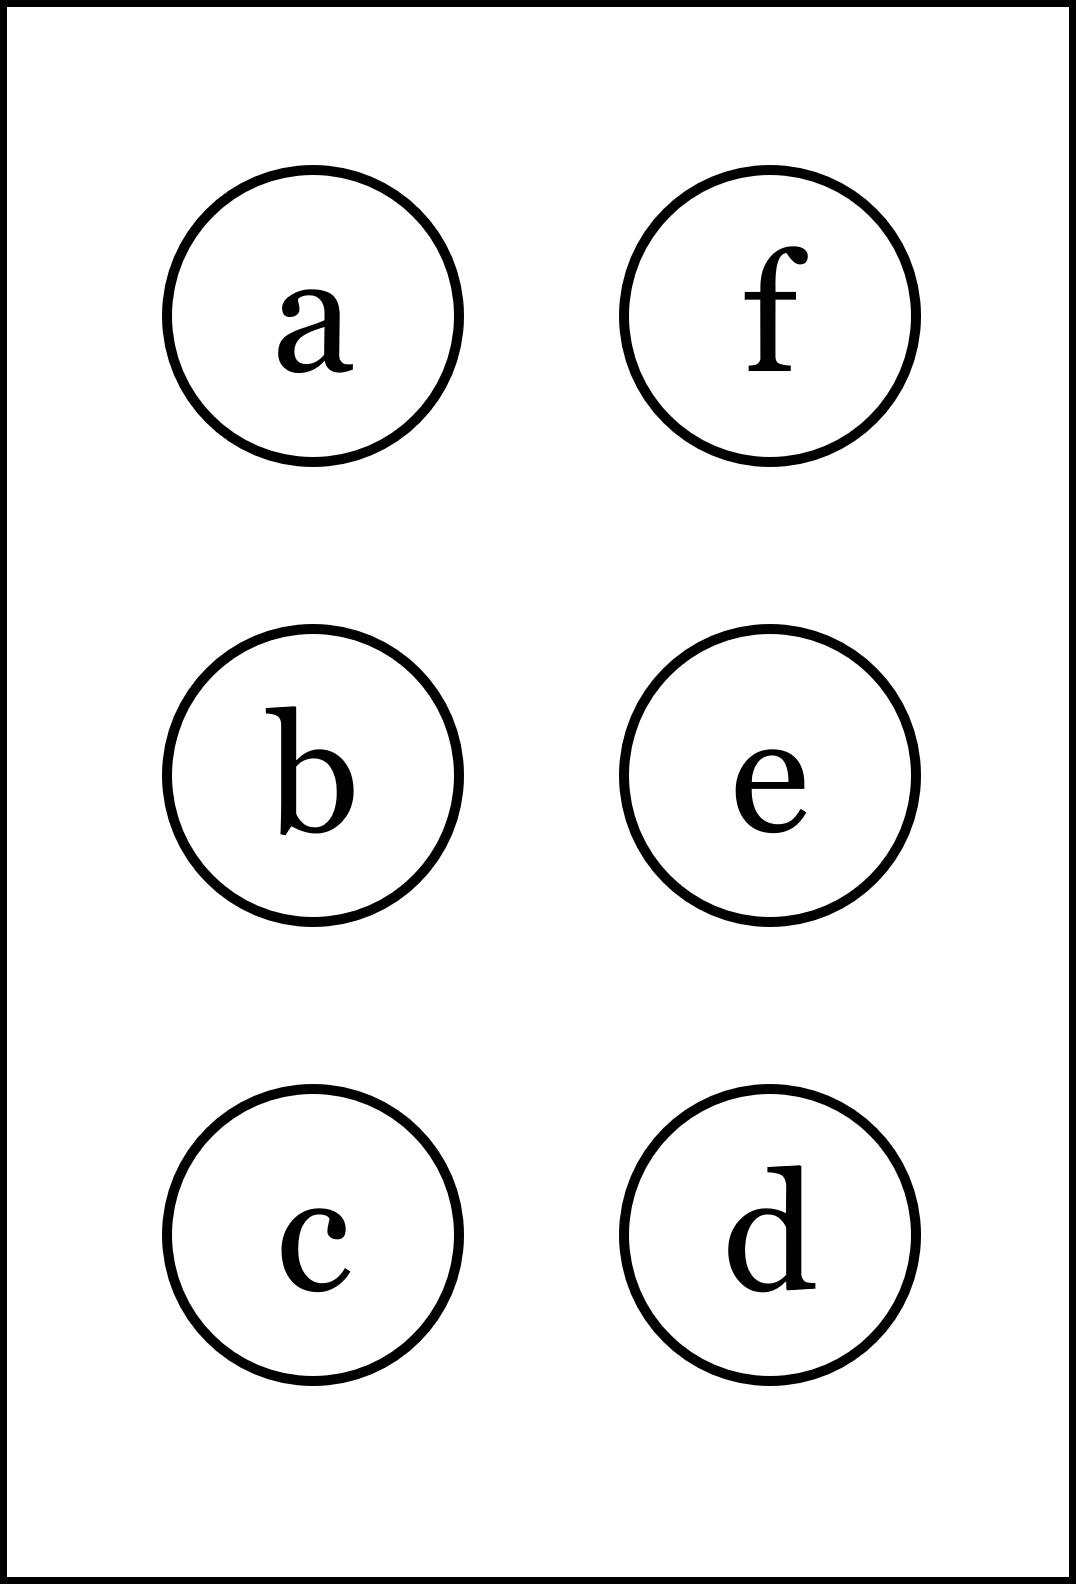
\includegraphics[height=40mm]{../images/braille.png}
{\small Písmeno Braillovej abecedy}
\end{center}
\end{minipage}
\end{center}
\end{minipage}
&
\begin{minipage}[c][104.5mm][t]{0.5\linewidth}
\begin{center}
\vspace{7mm}
{\huge Derivácie, skupina \textit{Mu $\mu$} -\romannumeral2}\\[5mm]
\textit{Meno:}\phantom{xxxxxxxxxxxxxxxxxxxxxxxxxxxxxxxxxxxxxxxxxxxxxxxxxxxxxxxxxxxxxxxxx}\\[5mm]
\begin{minipage}{0.95\linewidth}
\begin{center}
\textbf{Vypočítej derivace.} Pokud se výsledky shodují s těmi za otazníky,\\tak napravo obarvi příslušející kroužek načerno. \textbf{Spolu odevzdejte výsledné slovo}.
\end{center}
\end{minipage}
\\[1mm]
\begin{minipage}{0.79\linewidth}
\begin{center}
\begin{varwidth}{\linewidth}
\begin{enumerate}
\normalsize
\item $-3x^4-3x^3+5x^2+2x+4$\quad \dotfill\; ???\;\dotfill \quad $-3x^3-3x^2+5x+2$
\item $\cfrac{x^2-4x-5}{3x+1}$\quad \dotfill\; ???\;\dotfill \quad $\cfrac{3x^2+2x+11}{9x^2+6x+1}$
\item $\frac{-1}{x}\sqrt{9x+2}$\quad \dotfill\; ???\;\dotfill \quad $\frac{9x+4}{x^2 \sqrt{\smash[b]{9x+2}}}$
\item $e^{4x^2+x-1}$\quad \dotfill\; ???\;\dotfill \quad $e^{4x^2+x-1}$
\item $\ln{\left(\frac{4x+2}{9x-1}\right)}$\quad \dotfill\; ???\;\dotfill \quad $\frac{4}{4x+2}+\frac{9}{9x-1}$
\item $\frac{e^{-4x+8}}{-2x-1}$\quad \dotfill\; ???\;\dotfill \quad $\frac{8x+6}{(-2x-1)^2}e^{-4x+8}$
\end{enumerate}
\end{varwidth}
\end{center}
\end{minipage}
\begin{minipage}{0.20\linewidth}
\begin{center}
{\Huge\bfseries 2.} \\[2mm]
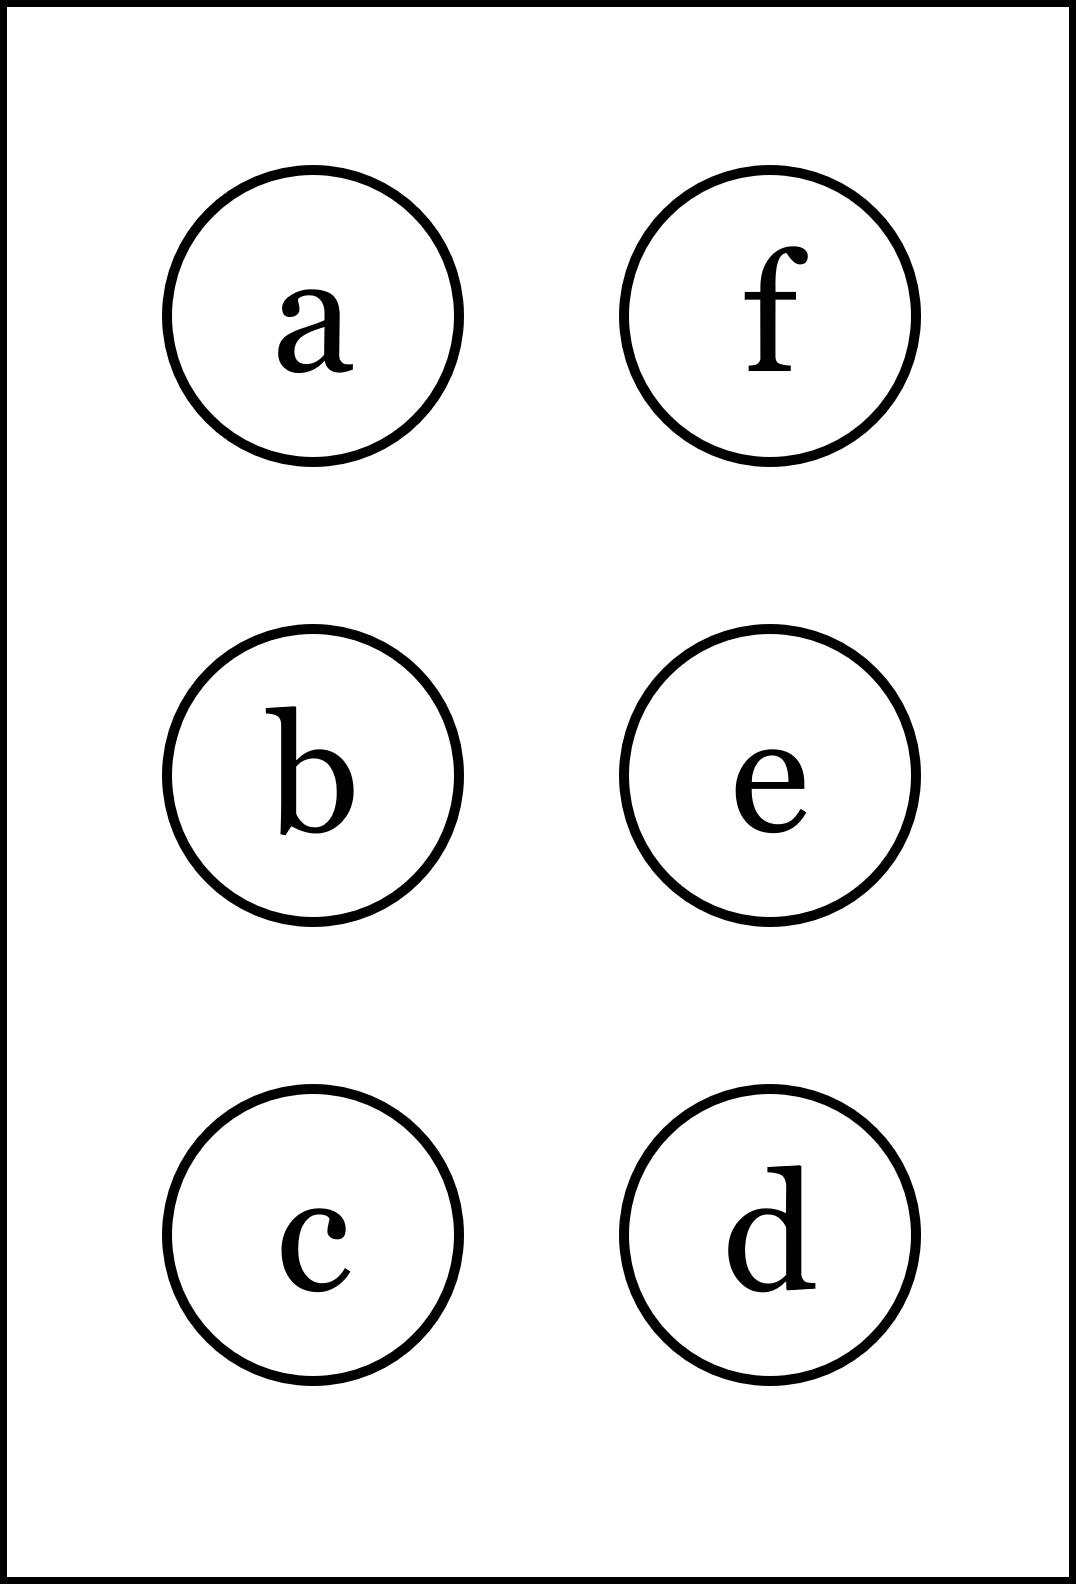
\includegraphics[height=40mm]{../images/braille.png}
{\small Písmeno Braillovej abecedy}
\end{center}
\end{minipage}
\end{center}
\end{minipage}
\\ \hdashline
\begin{minipage}[c][104.5mm][t]{0.5\linewidth}
\begin{center}
\vspace{7mm}
{\huge Derivácie, skupina \textit{Mu $\mu$} -\romannumeral3}\\[5mm]
\textit{Meno:}\phantom{xxxxxxxxxxxxxxxxxxxxxxxxxxxxxxxxxxxxxxxxxxxxxxxxxxxxxxxxxxxxxxxxx}\\[5mm]
\begin{minipage}{0.95\linewidth}
\begin{center}
\textbf{Vypočítej derivace.} Pokud se výsledky shodují s těmi za otazníky,\\tak napravo obarvi příslušející kroužek načerno. \textbf{Spolu odevzdejte výsledné slovo}.
\end{center}
\end{minipage}
\\[1mm]
\begin{minipage}{0.79\linewidth}
\begin{center}
\begin{varwidth}{\linewidth}
\begin{enumerate}
\normalsize
\item $-4x^4+3x^3+5x^2+2x+2$\quad \dotfill\; ???\;\dotfill \quad $-16x^3+9x^2+10x+2$
\item $\cfrac{4x^2-3x-6}{-4x+2}$\quad \dotfill\; ???\;\dotfill \quad $\cfrac{-16x^2+16x-30}{16x^2-16x+4}$
\item $\frac{-9}{x}\sqrt{-2x+1}$\quad \dotfill\; ???\;\dotfill \quad $\frac{-18x+18}{2x^2 \sqrt{\smash[b]{-2x+1}}}$
\item $e^{-2x^2-7x-3}$\quad \dotfill\; ???\;\dotfill \quad $(-4x-7)e^{-2x^2-7x-3}$
\item $\ln{\left(\frac{-9x-6}{-x-1}\right)}$\quad \dotfill\; ???\;\dotfill \quad $\frac{-9}{-9x-6}+\frac{-1}{-x-1}$
\item $\frac{e^{-4x+4}}{-2x-6}$\quad \dotfill\; ???\;\dotfill \quad $\frac{-8x+26}{(-2x-6)^2}e^{-4x+4}$
\end{enumerate}
\end{varwidth}
\end{center}
\end{minipage}
\begin{minipage}{0.20\linewidth}
\begin{center}
{\Huge\bfseries 3.} \\[2mm]
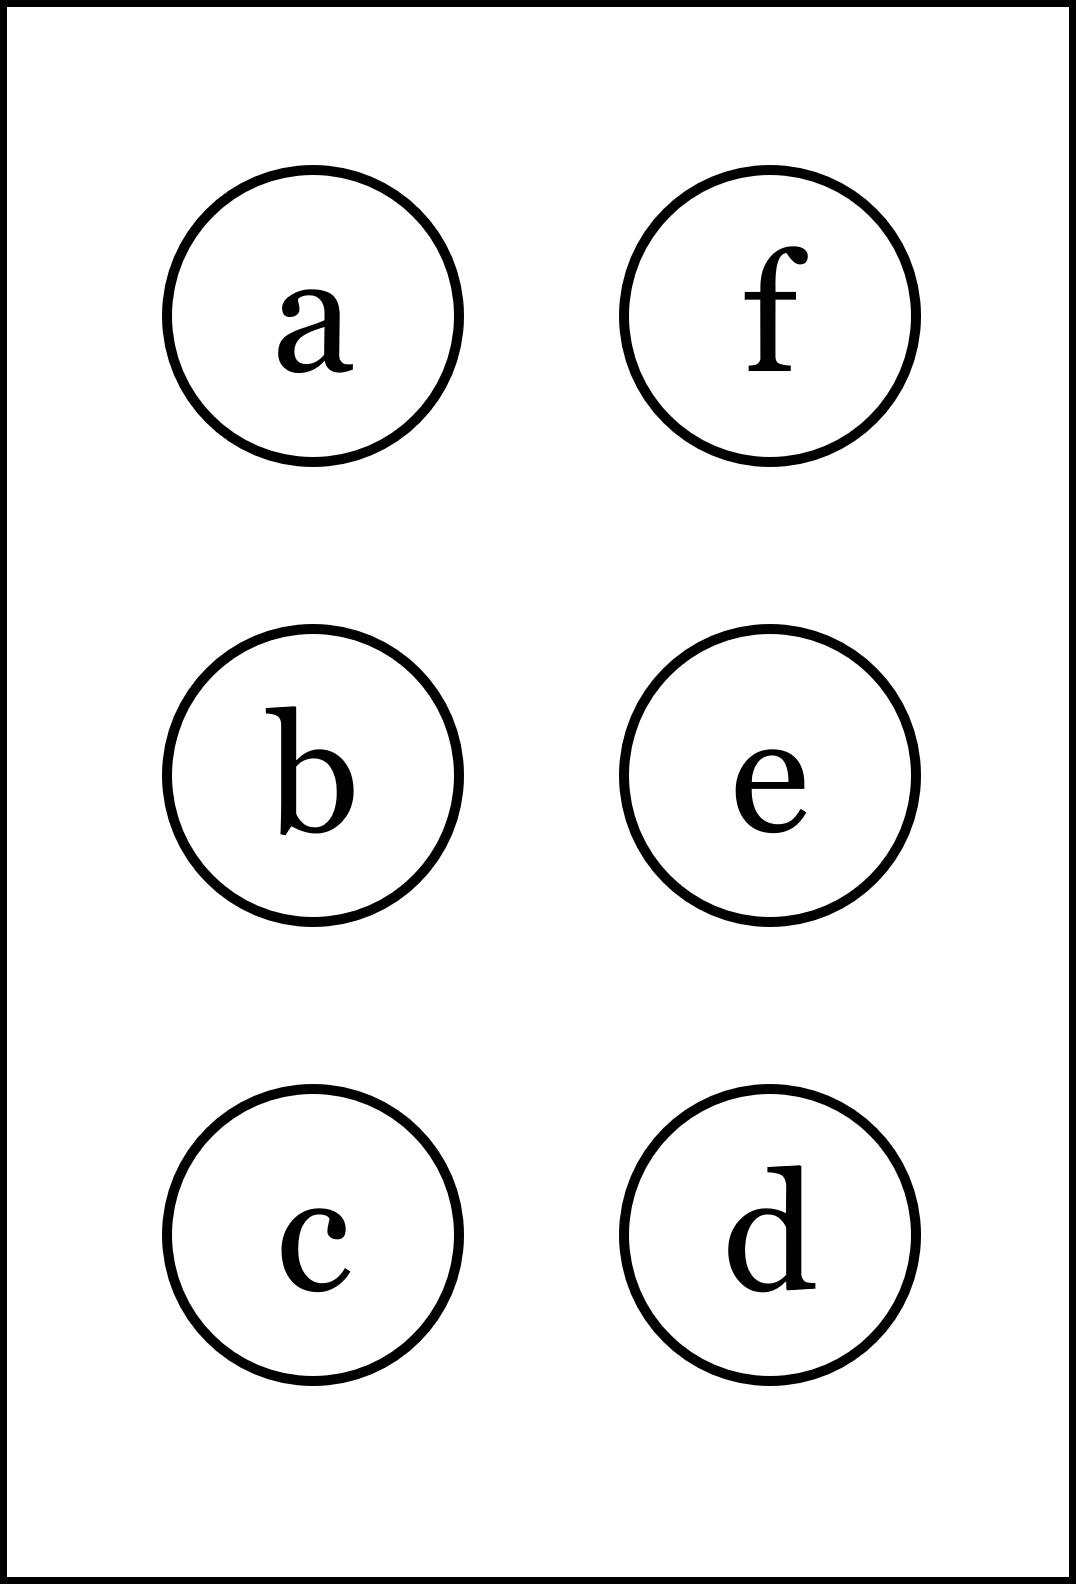
\includegraphics[height=40mm]{../images/braille.png}
{\small Písmeno Braillovej abecedy}
\end{center}
\end{minipage}
\end{center}
\end{minipage}
&
\begin{minipage}[c][104.5mm][t]{0.5\linewidth}
\begin{center}
\vspace{7mm}
{\huge Derivácie, skupina \textit{Mu $\mu$} -\romannumeral4}\\[5mm]
\textit{Meno:}\phantom{xxxxxxxxxxxxxxxxxxxxxxxxxxxxxxxxxxxxxxxxxxxxxxxxxxxxxxxxxxxxxxxxx}\\[5mm]
\begin{minipage}{0.95\linewidth}
\begin{center}
\textbf{Vypočítej derivace.} Pokud se výsledky shodují s těmi za otazníky,\\tak napravo obarvi příslušející kroužek načerno. \textbf{Spolu odevzdejte výsledné slovo}.
\end{center}
\end{minipage}
\\[1mm]
\begin{minipage}{0.79\linewidth}
\begin{center}
\begin{varwidth}{\linewidth}
\begin{enumerate}
\normalsize
\item $-3x^4+7x^3+3x^2-4x-1$\quad \dotfill\; ???\;\dotfill \quad $-12x^3+21x^2+6x-4$
\item $\cfrac{-2x^2+2x-2}{-5x+3}$\quad \dotfill\; ???\;\dotfill \quad $\cfrac{10x^2+12x-4}{25x^2-30x+9}$
\item $\frac{3}{x}\sqrt{3x-6}$\quad \dotfill\; ???\;\dotfill \quad $\frac{-9x+36}{2x^2 \sqrt{\smash[b]{3x-6}}}$
\item $e^{-7x^2+x+1}$\quad \dotfill\; ???\;\dotfill \quad $e^{-7x^2+x+1}$
\item $\ln{\left(\frac{7x-4}{5x-5}\right)}$\quad \dotfill\; ???\;\dotfill \quad $\frac{7}{7x-4}-\frac{5}{5x-5}$
\item $\frac{e^{8x+7}}{-5x-5}$\quad \dotfill\; ???\;\dotfill \quad $\frac{+40x-35}{(-5x-5)^2}e^{8x+7}$
\end{enumerate}
\end{varwidth}
\end{center}
\end{minipage}
\begin{minipage}{0.20\linewidth}
\begin{center}
{\Huge\bfseries 4.} \\[2mm]
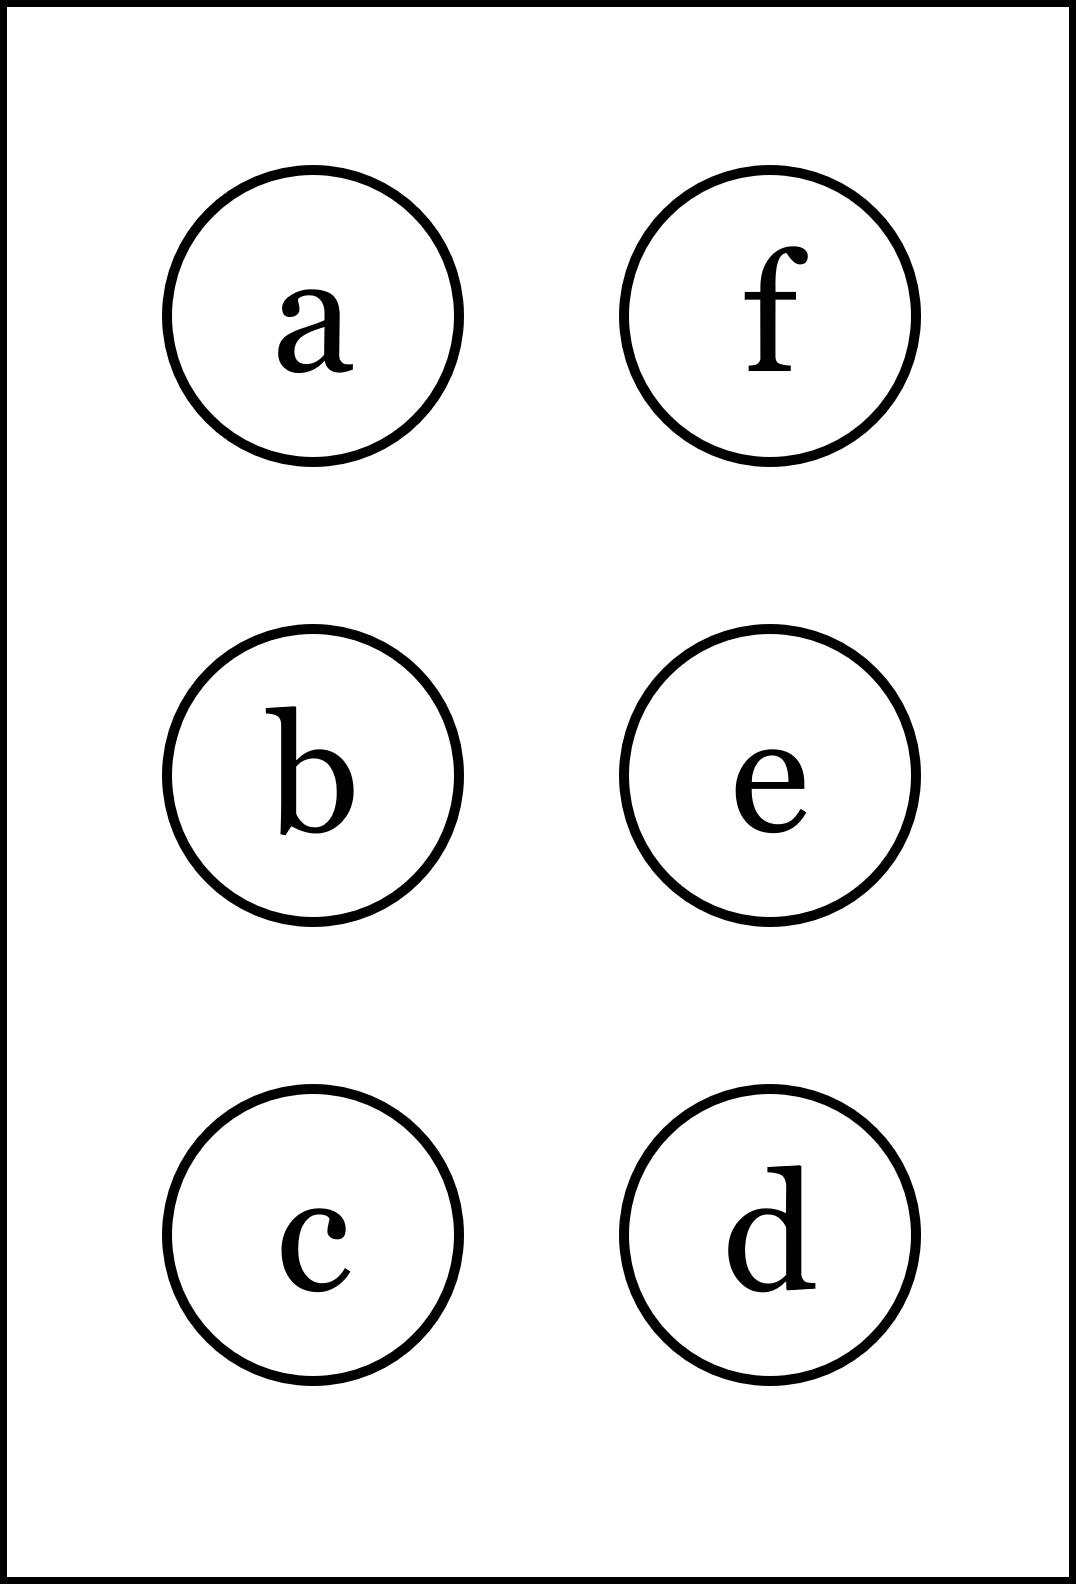
\includegraphics[height=40mm]{../images/braille.png}
{\small Písmeno Braillovej abecedy}
\end{center}
\end{minipage}
\end{center}
\end{minipage}
%
\end{tabular}
\newpage
\thispagestyle{empty}
\begin{tabular}{c:c}
\begin{minipage}[c][104.5mm][t]{0.5\linewidth}
\begin{center}
\vspace{7mm}
{\huge Derivácie, skupina \textit{Nu $\nu$} -\romannumeral1}\\[5mm]
\textit{Meno:}\phantom{xxxxxxxxxxxxxxxxxxxxxxxxxxxxxxxxxxxxxxxxxxxxxxxxxxxxxxxxxxxxxxxxx}\\[5mm]
\begin{minipage}{0.95\linewidth}
\begin{center}
\textbf{Vypočítej derivace.} Pokud se výsledky shodují s těmi za otazníky,\\tak napravo obarvi příslušející kroužek načerno. \textbf{Spolu odevzdejte výsledné slovo}.
\end{center}
\end{minipage}
\\[1mm]
\begin{minipage}{0.79\linewidth}
\begin{center}
\begin{varwidth}{\linewidth}
\begin{enumerate}
\normalsize
\item $6x^4-7x^3+8x^2-x+6$\quad \dotfill\; ???\;\dotfill \quad $24x^3-21x^2+16x-1$
\item $\cfrac{-5x^2-x-2}{-5x-1}$\quad \dotfill\; ???\;\dotfill \quad $\cfrac{25x^2-10x-9}{25x^2+10x+1}$
\item $\frac{-7}{x}\sqrt{3x+3}$\quad \dotfill\; ???\;\dotfill \quad $\frac{21x+42}{2x^2 \sqrt{\smash[b]{3x+3}}}$
\item $e^{x^2+3x+7}$\quad \dotfill\; ???\;\dotfill \quad $(2x+3)e^{x^2+3x+7}$
\item $\ln{\left(\frac{-8x+2}{-x-6}\right)}$\quad \dotfill\; ???\;\dotfill \quad $\frac{-8}{-8x+2}+\frac{-1}{-x-6}$
\item $\frac{e^{-8x+3}}{-2x-3}$\quad \dotfill\; ???\;\dotfill \quad $\frac{-16x+26}{(-2x-3)^2}e^{-8x+3}$
\end{enumerate}
\end{varwidth}
\end{center}
\end{minipage}
\begin{minipage}{0.20\linewidth}
\begin{center}
{\Huge\bfseries 1.} \\[2mm]
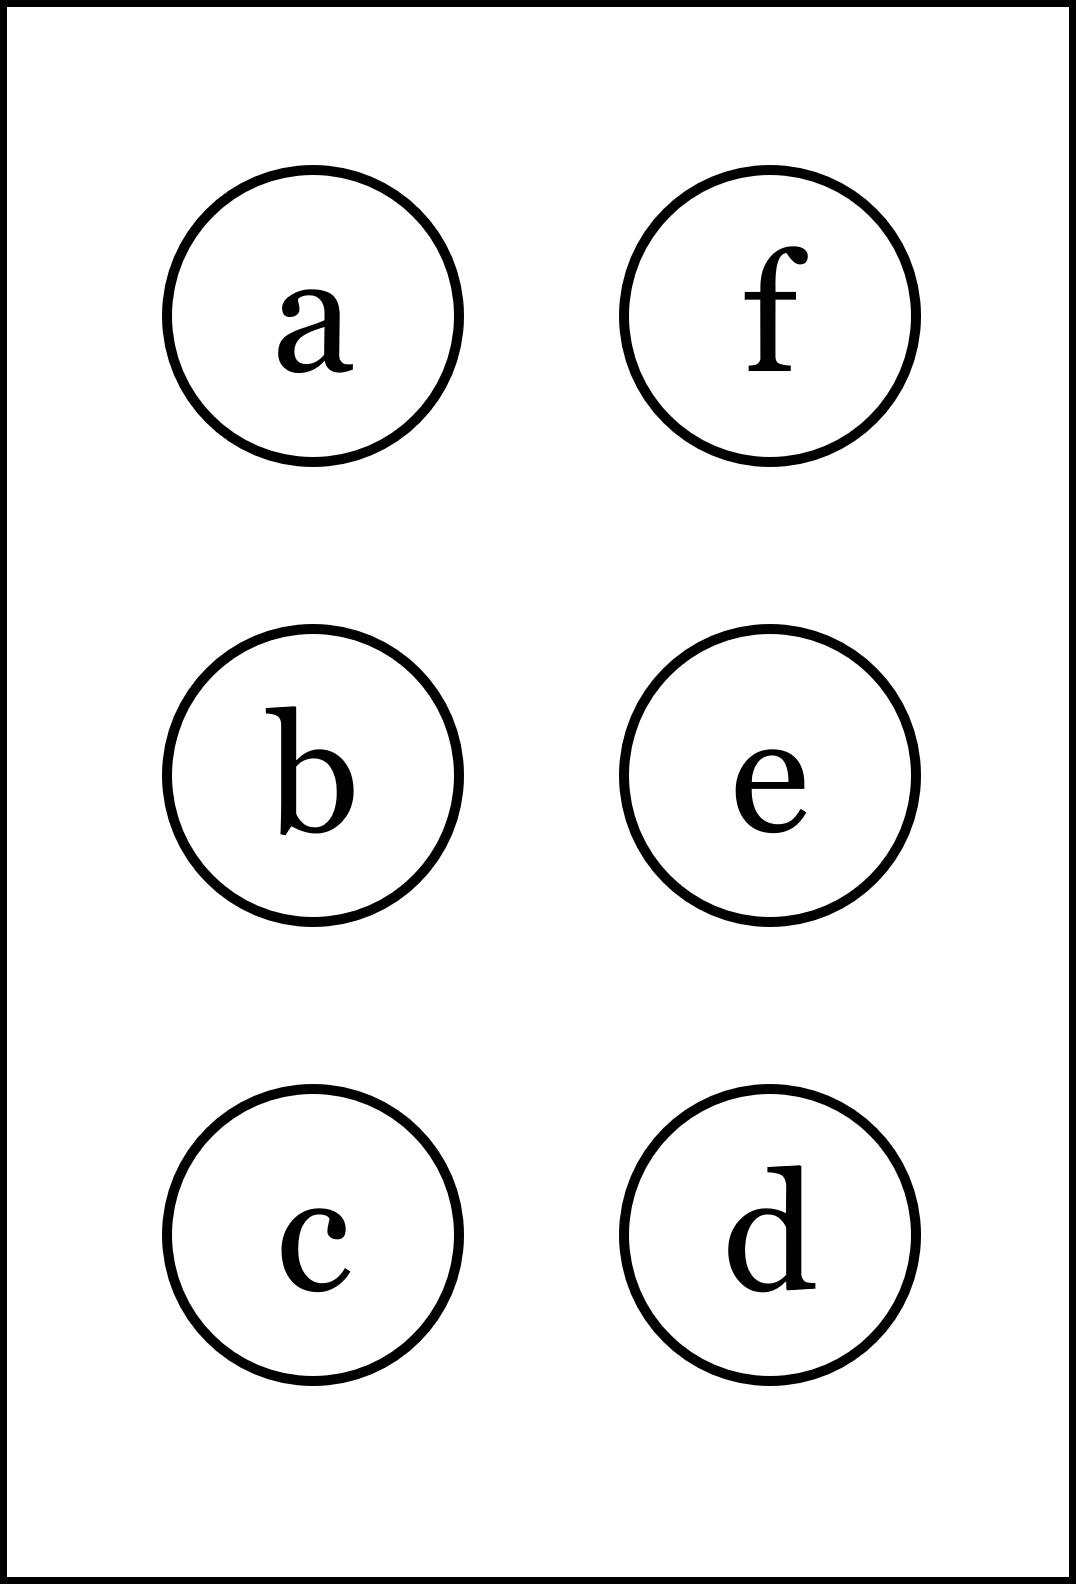
\includegraphics[height=40mm]{../images/braille.png}
{\small Písmeno Braillovej abecedy}
\end{center}
\end{minipage}
\end{center}
\end{minipage}
&
\begin{minipage}[c][104.5mm][t]{0.5\linewidth}
\begin{center}
\vspace{7mm}
{\huge Derivácie, skupina \textit{Nu $\nu$} -\romannumeral2}\\[5mm]
\textit{Meno:}\phantom{xxxxxxxxxxxxxxxxxxxxxxxxxxxxxxxxxxxxxxxxxxxxxxxxxxxxxxxxxxxxxxxxx}\\[5mm]
\begin{minipage}{0.95\linewidth}
\begin{center}
\textbf{Vypočítej derivace.} Pokud se výsledky shodují s těmi za otazníky,\\tak napravo obarvi příslušející kroužek načerno. \textbf{Spolu odevzdejte výsledné slovo}.
\end{center}
\end{minipage}
\\[1mm]
\begin{minipage}{0.79\linewidth}
\begin{center}
\begin{varwidth}{\linewidth}
\begin{enumerate}
\normalsize
\item $-3x^4+5x^3+2x^2+3x+1$\quad \dotfill\; ???\;\dotfill \quad $-12x^3+15x^2+4x+3$
\item $\cfrac{2x^2-2x+5}{4x+4}$\quad \dotfill\; ???\;\dotfill \quad $\cfrac{8x^2+16x-28}{16x^2+32x+16}$
\item $\frac{-6}{x}\sqrt{-6x-6}$\quad \dotfill\; ???\;\dotfill \quad $\frac{-36x-72}{2x^2 \sqrt{\smash[b]{-6x-6}}}$
\item $e^{-x^2+7x+1}$\quad \dotfill\; ???\;\dotfill \quad $e^{-x^2+7x+1}$
\item $\ln{\left(\frac{-x-3}{-5x-4}\right)}$\quad \dotfill\; ???\;\dotfill \quad $\frac{-1}{-x-3}-\frac{-5}{-5x-4}$
\item $\frac{e^{-x-5}}{2x+7}$\quad \dotfill\; ???\;\dotfill \quad $\frac{+2x-9}{(2x+7)^2}e^{-x-5}$
\end{enumerate}
\end{varwidth}
\end{center}
\end{minipage}
\begin{minipage}{0.20\linewidth}
\begin{center}
{\Huge\bfseries 2.} \\[2mm]
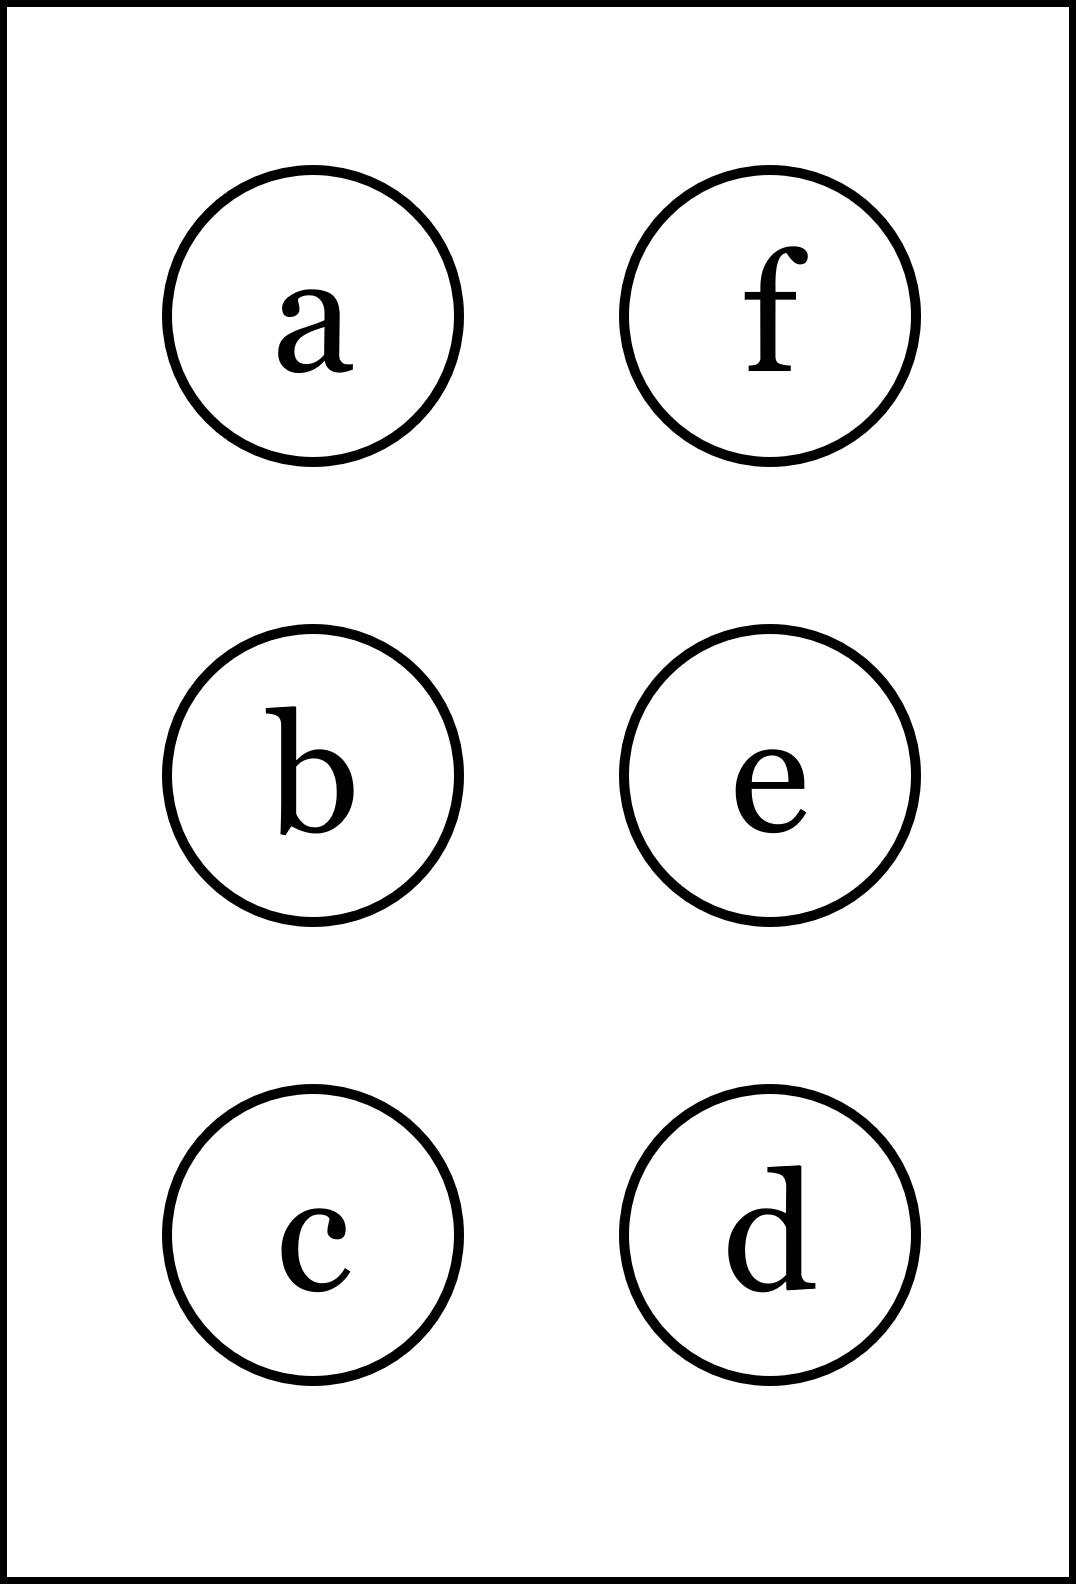
\includegraphics[height=40mm]{../images/braille.png}
{\small Písmeno Braillovej abecedy}
\end{center}
\end{minipage}
\end{center}
\end{minipage}
\\ \hdashline
\begin{minipage}[c][104.5mm][t]{0.5\linewidth}
\begin{center}
\vspace{7mm}
{\huge Derivácie, skupina \textit{Nu $\nu$} -\romannumeral3}\\[5mm]
\textit{Meno:}\phantom{xxxxxxxxxxxxxxxxxxxxxxxxxxxxxxxxxxxxxxxxxxxxxxxxxxxxxxxxxxxxxxxxx}\\[5mm]
\begin{minipage}{0.95\linewidth}
\begin{center}
\textbf{Vypočítej derivace.} Pokud se výsledky shodují s těmi za otazníky,\\tak napravo obarvi příslušející kroužek načerno. \textbf{Spolu odevzdejte výsledné slovo}.
\end{center}
\end{minipage}
\\[1mm]
\begin{minipage}{0.79\linewidth}
\begin{center}
\begin{varwidth}{\linewidth}
\begin{enumerate}
\normalsize
\item $-5x^4+2x^3-3x^2-5x-3$\quad \dotfill\; ???\;\dotfill \quad $-20x^3+6x^2-6x-5$
\item $\cfrac{4x^2+3x-2}{-x-5}$\quad \dotfill\; ???\;\dotfill \quad $\cfrac{-4x^2+40x-17}{x^2+10x+25}$
\item $\frac{-1}{x}\sqrt{-2x-2}$\quad \dotfill\; ???\;\dotfill \quad $\frac{-2x-4}{x^2 \sqrt{\smash[b]{-2x-2}}}$
\item $e^{-2x^2-5x-2}$\quad \dotfill\; ???\;\dotfill \quad $e^{-2x^2-5x-2}$
\item $\ln{\left(\frac{8x-5}{3x+3}\right)}$\quad \dotfill\; ???\;\dotfill \quad $\frac{8}{8x-5}+\frac{3}{3x+3}$
\item $\frac{e^{2x+2}}{-2x+1}$\quad \dotfill\; ???\;\dotfill \quad $\frac{+4x+4}{(-2x+1)^2}e^{2x+2}$
\end{enumerate}
\end{varwidth}
\end{center}
\end{minipage}
\begin{minipage}{0.20\linewidth}
\begin{center}
{\Huge\bfseries 3.} \\[2mm]
\includegraphics[height=40mm]{../images/braille.png}
{\small Písmeno Braillovej abecedy}
\end{center}
\end{minipage}
\end{center}
\end{minipage}
&
\begin{minipage}[c][104.5mm][t]{0.5\linewidth}
\begin{center}
\vspace{7mm}
{\huge Derivácie, skupina \textit{Nu $\nu$} -\romannumeral4}\\[5mm]
\textit{Meno:}\phantom{xxxxxxxxxxxxxxxxxxxxxxxxxxxxxxxxxxxxxxxxxxxxxxxxxxxxxxxxxxxxxxxxx}\\[5mm]
\begin{minipage}{0.95\linewidth}
\begin{center}
\textbf{Vypočítej derivace.} Pokud se výsledky shodují s těmi za otazníky,\\tak napravo obarvi příslušející kroužek načerno. \textbf{Spolu odevzdejte výsledné slovo}.
\end{center}
\end{minipage}
\\[1mm]
\begin{minipage}{0.79\linewidth}
\begin{center}
\begin{varwidth}{\linewidth}
\begin{enumerate}
\normalsize
\item $9x^4-3x^3+4x^2-x+2$\quad \dotfill\; ???\;\dotfill \quad $36x^3-9x^2+8x-1$
\item $\cfrac{2x^2+2x-2}{2x-4}$\quad \dotfill\; ???\;\dotfill \quad $\cfrac{4x^2+16x-4}{4x^2-16x+16}$
\item $\frac{6}{x}\sqrt{-2x-3}$\quad \dotfill\; ???\;\dotfill \quad $\frac{12x+36}{2x^2 \sqrt{\smash[b]{-2x-3}}}$
\item $e^{2x^2-5x-3}$\quad \dotfill\; ???\;\dotfill \quad $e^{2x^2-5x-3}$
\item $\ln{\left(\frac{-6x-2}{3x+5}\right)}$\quad \dotfill\; ???\;\dotfill \quad $\frac{-6}{-6x-2}-\frac{3}{3x+5}$
\item $\frac{e^{-3x-4}}{-6x+2}$\quad \dotfill\; ???\;\dotfill \quad $\frac{18x+0}{(-6x+2)^2}e^{-3x-4}$
\end{enumerate}
\end{varwidth}
\end{center}
\end{minipage}
\begin{minipage}{0.20\linewidth}
\begin{center}
{\Huge\bfseries 4.} \\[2mm]
\includegraphics[height=40mm]{../images/braille.png}
{\small Písmeno Braillovej abecedy}
\end{center}
\end{minipage}
\end{center}
\end{minipage}
%
\end{tabular}
\newpage
\thispagestyle{empty}
\begin{tabular}{c:c}
\begin{minipage}[c][104.5mm][t]{0.5\linewidth}
\begin{center}
\vspace{7mm}
{\huge Derivácie, skupina \textit{Xi $\xi$} -\romannumeral1}\\[5mm]
\textit{Meno:}\phantom{xxxxxxxxxxxxxxxxxxxxxxxxxxxxxxxxxxxxxxxxxxxxxxxxxxxxxxxxxxxxxxxxx}\\[5mm]
\begin{minipage}{0.95\linewidth}
\begin{center}
\textbf{Vypočítej derivace.} Pokud se výsledky shodují s těmi za otazníky,\\tak napravo obarvi příslušející kroužek načerno. \textbf{Spolu odevzdejte výsledné slovo}.
\end{center}
\end{minipage}
\\[1mm]
\begin{minipage}{0.79\linewidth}
\begin{center}
\begin{varwidth}{\linewidth}
\begin{enumerate}
\normalsize
\item $-x^4+6x^3-5x^2-2x+4$\quad \dotfill\; ???\;\dotfill \quad $-4x^3+18x^2-10x-2$
\item $\cfrac{-4x^2+3x+2}{6x-3}$\quad \dotfill\; ???\;\dotfill \quad $\cfrac{-24x^2-24x-21}{36x^2-36x+9}$
\item $\frac{-6}{x}\sqrt{-7x-2}$\quad \dotfill\; ???\;\dotfill \quad $\frac{-42x-24}{x^2 \sqrt{\smash[b]{-7x-2}}}$
\item $e^{-2x^2+4x+5}$\quad \dotfill\; ???\;\dotfill \quad $e^{-2x^2+4x+5}$
\item $\ln{\left(\frac{7x+1}{4x+4}\right)}$\quad \dotfill\; ???\;\dotfill \quad $\frac{7}{7x+1}-\frac{4}{4x+4}$
\item $\frac{e^{-7x-5}}{9x+1}$\quad \dotfill\; ???\;\dotfill \quad $\frac{-63x-16}{(9x+1)^2}e^{-7x-5}$
\end{enumerate}
\end{varwidth}
\end{center}
\end{minipage}
\begin{minipage}{0.20\linewidth}
\begin{center}
{\Huge\bfseries 1.} \\[2mm]
\includegraphics[height=40mm]{../images/braille.png}
{\small Písmeno Braillovej abecedy}
\end{center}
\end{minipage}
\end{center}
\end{minipage}
&
\begin{minipage}[c][104.5mm][t]{0.5\linewidth}
\begin{center}
\vspace{7mm}
{\huge Derivácie, skupina \textit{Xi $\xi$} -\romannumeral2}\\[5mm]
\textit{Meno:}\phantom{xxxxxxxxxxxxxxxxxxxxxxxxxxxxxxxxxxxxxxxxxxxxxxxxxxxxxxxxxxxxxxxxx}\\[5mm]
\begin{minipage}{0.95\linewidth}
\begin{center}
\textbf{Vypočítej derivace.} Pokud se výsledky shodují s těmi za otazníky,\\tak napravo obarvi příslušející kroužek načerno. \textbf{Spolu odevzdejte výsledné slovo}.
\end{center}
\end{minipage}
\\[1mm]
\begin{minipage}{0.79\linewidth}
\begin{center}
\begin{varwidth}{\linewidth}
\begin{enumerate}
\normalsize
\item $-x^4-3x^3+x^2+8x+6$\quad \dotfill\; ???\;\dotfill \quad $-4x^3-9x^2+2x+8$
\item $\cfrac{3x^2-3x-6}{2x-5}$\quad \dotfill\; ???\;\dotfill \quad $\cfrac{6x^2-30x+27}{4x^2-20x+25}$
\item $\frac{4}{x}\sqrt{-3x-6}$\quad \dotfill\; ???\;\dotfill \quad $\frac{12x+48}{2x^2 \sqrt{\smash[b]{-3x-6}}}$
\item $e^{2x^2+3x+9}$\quad \dotfill\; ???\;\dotfill \quad $e^{2x^2+3x+9}$
\item $\ln{\left(\frac{-8x-2}{6x-1}\right)}$\quad \dotfill\; ???\;\dotfill \quad $\frac{-8}{-8x-2}-\frac{6}{6x-1}$
\item $\frac{e^{-5x+2}}{2x+3}$\quad \dotfill\; ???\;\dotfill \quad $\frac{+10x-17}{(2x+3)^2}e^{-5x+2}$
\end{enumerate}
\end{varwidth}
\end{center}
\end{minipage}
\begin{minipage}{0.20\linewidth}
\begin{center}
{\Huge\bfseries 2.} \\[2mm]
\includegraphics[height=40mm]{../images/braille.png}
{\small Písmeno Braillovej abecedy}
\end{center}
\end{minipage}
\end{center}
\end{minipage}
\\ \hdashline
\begin{minipage}[c][104.5mm][t]{0.5\linewidth}
\begin{center}
\vspace{7mm}
{\huge Derivácie, skupina \textit{Xi $\xi$} -\romannumeral3}\\[5mm]
\textit{Meno:}\phantom{xxxxxxxxxxxxxxxxxxxxxxxxxxxxxxxxxxxxxxxxxxxxxxxxxxxxxxxxxxxxxxxxx}\\[5mm]
\begin{minipage}{0.95\linewidth}
\begin{center}
\textbf{Vypočítej derivace.} Pokud se výsledky shodují s těmi za otazníky,\\tak napravo obarvi příslušející kroužek načerno. \textbf{Spolu odevzdejte výsledné slovo}.
\end{center}
\end{minipage}
\\[1mm]
\begin{minipage}{0.79\linewidth}
\begin{center}
\begin{varwidth}{\linewidth}
\begin{enumerate}
\normalsize
\item $-4x^4+6x^3+x^2+6x-7$\quad \dotfill\; ???\;\dotfill \quad $-16x^3+18x^2+2x+6$
\item $\cfrac{-6x^2+2x+2}{-3x+4}$\quad \dotfill\; ???\;\dotfill \quad $\cfrac{18x^2+48x+14}{9x^2-24x+16}$
\item $\frac{1}{x}\sqrt{9x-4}$\quad \dotfill\; ???\;\dotfill \quad $\frac{-9x+8}{x^2 \sqrt{\smash[b]{9x-4}}}$
\item $e^{9x^2-6x-6}$\quad \dotfill\; ???\;\dotfill \quad $e^{9x^2-6x-6}$
\item $\ln{\left(\frac{-2x-3}{x+2}\right)}$\quad \dotfill\; ???\;\dotfill \quad $\frac{-2}{-2x-3}+\frac{1}{x+2}$
\item $\frac{e^{3x+3}}{8x-2}$\quad \dotfill\; ???\;\dotfill \quad $\frac{-24x-14}{(8x-2)^2}e^{3x+3}$
\end{enumerate}
\end{varwidth}
\end{center}
\end{minipage}
\begin{minipage}{0.20\linewidth}
\begin{center}
{\Huge\bfseries 3.} \\[2mm]
\includegraphics[height=40mm]{../images/braille.png}
{\small Písmeno Braillovej abecedy}
\end{center}
\end{minipage}
\end{center}
\end{minipage}
&
\begin{minipage}[c][104.5mm][t]{0.5\linewidth}
\begin{center}
\vspace{7mm}
{\huge Derivácie, skupina \textit{Xi $\xi$} -\romannumeral4}\\[5mm]
\textit{Meno:}\phantom{xxxxxxxxxxxxxxxxxxxxxxxxxxxxxxxxxxxxxxxxxxxxxxxxxxxxxxxxxxxxxxxxx}\\[5mm]
\begin{minipage}{0.95\linewidth}
\begin{center}
\textbf{Vypočítej derivace.} Pokud se výsledky shodují s těmi za otazníky,\\tak napravo obarvi příslušející kroužek načerno. \textbf{Spolu odevzdejte výsledné slovo}.
\end{center}
\end{minipage}
\\[1mm]
\begin{minipage}{0.79\linewidth}
\begin{center}
\begin{varwidth}{\linewidth}
\begin{enumerate}
\normalsize
\item $6x^4-x^3-2x^2+7x-1$\quad \dotfill\; ???\;\dotfill \quad $24x^3-3x^2-4x+7$
\item $\cfrac{-2x^2+x+1}{2x-1}$\quad \dotfill\; ???\;\dotfill \quad $\cfrac{-4x^2-4x-3}{4x^2-4x+1}$
\item $\frac{-5}{x}\sqrt{5x+2}$\quad \dotfill\; ???\;\dotfill \quad $\frac{25x+20}{2x^2 \sqrt{\smash[b]{5x+2}}}$
\item $e^{-9x^2-5x+9}$\quad \dotfill\; ???\;\dotfill \quad $e^{-9x^2-5x+9}$
\item $\ln{\left(\frac{-4x+4}{-x+1}\right)}$\quad \dotfill\; ???\;\dotfill \quad $\frac{-4}{-4x+4}+\frac{-1}{-x+1}$
\item $\frac{e^{-x-9}}{-8x-2}$\quad \dotfill\; ???\;\dotfill \quad $\frac{-8x+10}{(-8x-2)^2}e^{-x-9}$
\end{enumerate}
\end{varwidth}
\end{center}
\end{minipage}
\begin{minipage}{0.20\linewidth}
\begin{center}
{\Huge\bfseries 4.} \\[2mm]
\includegraphics[height=40mm]{../images/braille.png}
{\small Písmeno Braillovej abecedy}
\end{center}
\end{minipage}
\end{center}
\end{minipage}
%
\end{tabular}
\newpage
\thispagestyle{empty}
\begin{tabular}{c:c}
\begin{minipage}[c][104.5mm][t]{0.5\linewidth}
\begin{center}
\vspace{7mm}
{\huge Derivácie, skupina \textit{Omicron $\omicron$} -\romannumeral1}\\[5mm]
\textit{Meno:}\phantom{xxxxxxxxxxxxxxxxxxxxxxxxxxxxxxxxxxxxxxxxxxxxxxxxxxxxxxxxxxxxxxxxx}\\[5mm]
\begin{minipage}{0.95\linewidth}
\begin{center}
\textbf{Vypočítej derivace.} Pokud se výsledky shodují s těmi za otazníky,\\tak napravo obarvi příslušející kroužek načerno. \textbf{Spolu odevzdejte výsledné slovo}.
\end{center}
\end{minipage}
\\[1mm]
\begin{minipage}{0.79\linewidth}
\begin{center}
\begin{varwidth}{\linewidth}
\begin{enumerate}
\normalsize
\item $-3x^4-x^3+8x^2-3x+5$\quad \dotfill\; ???\;\dotfill \quad $-12x^3-3x^2+16x-3$
\item $\cfrac{-5x^2-4x-2}{6x-3}$\quad \dotfill\; ???\;\dotfill \quad $\cfrac{-30x^2+30x+24}{36x^2-36x+9}$
\item $\frac{-9}{x}\sqrt{-5x-2}$\quad \dotfill\; ???\;\dotfill \quad $\frac{-45x-36}{x^2 \sqrt{\smash[b]{-5x-2}}}$
\item $e^{x^2+4x+2}$\quad \dotfill\; ???\;\dotfill \quad $e^{x^2+4x+2}$
\item $\ln{\left(\frac{3x-6}{-5x+2}\right)}$\quad \dotfill\; ???\;\dotfill \quad $\frac{3}{3x-6}+\frac{-5}{-5x+2}$
\item $\frac{e^{-7x+8}}{-x+1}$\quad \dotfill\; ???\;\dotfill \quad $\frac{7x-6}{(-x+1)^2}e^{-7x+8}$
\end{enumerate}
\end{varwidth}
\end{center}
\end{minipage}
\begin{minipage}{0.20\linewidth}
\begin{center}
{\Huge\bfseries 1.} \\[2mm]
\includegraphics[height=40mm]{../images/braille.png}
{\small Písmeno Braillovej abecedy}
\end{center}
\end{minipage}
\end{center}
\end{minipage}
&
\begin{minipage}[c][104.5mm][t]{0.5\linewidth}
\begin{center}
\vspace{7mm}
{\huge Derivácie, skupina \textit{Omicron $\omicron$} -\romannumeral2}\\[5mm]
\textit{Meno:}\phantom{xxxxxxxxxxxxxxxxxxxxxxxxxxxxxxxxxxxxxxxxxxxxxxxxxxxxxxxxxxxxxxxxx}\\[5mm]
\begin{minipage}{0.95\linewidth}
\begin{center}
\textbf{Vypočítej derivace.} Pokud se výsledky shodují s těmi za otazníky,\\tak napravo obarvi příslušející kroužek načerno. \textbf{Spolu odevzdejte výsledné slovo}.
\end{center}
\end{minipage}
\\[1mm]
\begin{minipage}{0.79\linewidth}
\begin{center}
\begin{varwidth}{\linewidth}
\begin{enumerate}
\normalsize
\item $2x^4-x^3+7x^2+5x+1$\quad \dotfill\; ???\;\dotfill \quad $2x^3-x^2+7x+5$
\item $\cfrac{6x^2+x-2}{3x+2}$\quad \dotfill\; ???\;\dotfill \quad $\cfrac{18x^2+24x+8}{9x^2+12x+4}$
\item $\frac{5}{x}\sqrt{-x-9}$\quad \dotfill\; ???\;\dotfill \quad $\frac{5x+90}{x^2 \sqrt{\smash[b]{-x-9}}}$
\item $e^{-3x^2+2x+1}$\quad \dotfill\; ???\;\dotfill \quad $e^{-3x^2+2x+1}$
\item $\ln{\left(\frac{-6x-5}{5x+1}\right)}$\quad \dotfill\; ???\;\dotfill \quad $\frac{-6}{-6x-5}+\frac{5}{5x+1}$
\item $\frac{e^{2x-2}}{3x+2}$\quad \dotfill\; ???\;\dotfill \quad $\frac{6x+1}{(3x+2)^2}e^{2x-2}$
\end{enumerate}
\end{varwidth}
\end{center}
\end{minipage}
\begin{minipage}{0.20\linewidth}
\begin{center}
{\Huge\bfseries 2.} \\[2mm]
\includegraphics[height=40mm]{../images/braille.png}
{\small Písmeno Braillovej abecedy}
\end{center}
\end{minipage}
\end{center}
\end{minipage}
\\ \hdashline
\begin{minipage}[c][104.5mm][t]{0.5\linewidth}
\begin{center}
\vspace{7mm}
{\huge Derivácie, skupina \textit{Omicron $\omicron$} -\romannumeral3}\\[5mm]
\textit{Meno:}\phantom{xxxxxxxxxxxxxxxxxxxxxxxxxxxxxxxxxxxxxxxxxxxxxxxxxxxxxxxxxxxxxxxxx}\\[5mm]
\begin{minipage}{0.95\linewidth}
\begin{center}
\textbf{Vypočítej derivace.} Pokud se výsledky shodují s těmi za otazníky,\\tak napravo obarvi příslušející kroužek načerno. \textbf{Spolu odevzdejte výsledné slovo}.
\end{center}
\end{minipage}
\\[1mm]
\begin{minipage}{0.79\linewidth}
\begin{center}
\begin{varwidth}{\linewidth}
\begin{enumerate}
\normalsize
\item $-x^4-x^3+5x^2+5x-8$\quad \dotfill\; ???\;\dotfill \quad $-4x^3-3x^2+10x+5$
\item $\cfrac{5x^2+2x-1}{3x-3}$\quad \dotfill\; ???\;\dotfill \quad $\cfrac{15x^2-30x-3}{9x^2-18x+9}$
\item $\frac{-5}{x}\sqrt{-5x-5}$\quad \dotfill\; ???\;\dotfill \quad $\frac{-25x-50}{2x^2 \sqrt{\smash[b]{-5x-5}}}$
\item $e^{7x^2+8x+3}$\quad \dotfill\; ???\;\dotfill \quad $e^{7x^2+8x+3}$
\item $\ln{\left(\frac{3x+3}{x-3}\right)}$\quad \dotfill\; ???\;\dotfill \quad $\frac{3}{3x+3}+\frac{1}{x-3}$
\item $\frac{e^{7x-5}}{-6x+4}$\quad \dotfill\; ???\;\dotfill \quad $\frac{+42x+34}{(-6x+4)^2}e^{7x-5}$
\end{enumerate}
\end{varwidth}
\end{center}
\end{minipage}
\begin{minipage}{0.20\linewidth}
\begin{center}
{\Huge\bfseries 3.} \\[2mm]
\includegraphics[height=40mm]{../images/braille.png}
{\small Písmeno Braillovej abecedy}
\end{center}
\end{minipage}
\end{center}
\end{minipage}
&
\begin{minipage}[c][104.5mm][t]{0.5\linewidth}
\begin{center}
\vspace{7mm}
{\huge Derivácie, skupina \textit{Omicron $\omicron$} -\romannumeral4}\\[5mm]
\textit{Meno:}\phantom{xxxxxxxxxxxxxxxxxxxxxxxxxxxxxxxxxxxxxxxxxxxxxxxxxxxxxxxxxxxxxxxxx}\\[5mm]
\begin{minipage}{0.95\linewidth}
\begin{center}
\textbf{Vypočítej derivace.} Pokud se výsledky shodují s těmi za otazníky,\\tak napravo obarvi příslušející kroužek načerno. \textbf{Spolu odevzdejte výsledné slovo}.
\end{center}
\end{minipage}
\\[1mm]
\begin{minipage}{0.79\linewidth}
\begin{center}
\begin{varwidth}{\linewidth}
\begin{enumerate}
\normalsize
\item $3x^4+5x^3+5x^2+5x+1$\quad \dotfill\; ???\;\dotfill \quad $12x^3+15x^2+10x+5$
\item $\cfrac{x^2+x-3}{2x+1}$\quad \dotfill\; ???\;\dotfill \quad $\cfrac{2x^2-2x+7}{4x^2+4x+1}$
\item $\frac{2}{x}\sqrt{8x+5}$\quad \dotfill\; ???\;\dotfill \quad $\frac{-16x-20}{2x^2 \sqrt{\smash[b]{8x+5}}}$
\item $e^{9x^2+2x+9}$\quad \dotfill\; ???\;\dotfill \quad $e^{9x^2+2x+9}$
\item $\ln{\left(\frac{7x+1}{-8x+2}\right)}$\quad \dotfill\; ???\;\dotfill \quad $\frac{7}{7x+1}+\frac{-8}{-8x+2}$
\item $\frac{e^{-x+4}}{7x+4}$\quad \dotfill\; ???\;\dotfill \quad $\frac{-7x-11}{(7x+4)^2}e^{-x+4}$
\end{enumerate}
\end{varwidth}
\end{center}
\end{minipage}
\begin{minipage}{0.20\linewidth}
\begin{center}
{\Huge\bfseries 4.} \\[2mm]
\includegraphics[height=40mm]{../images/braille.png}
{\small Písmeno Braillovej abecedy}
\end{center}
\end{minipage}
\end{center}
\end{minipage}
%
\end{tabular}
\newpage
\thispagestyle{empty}
\begin{tabular}{c:c}
\begin{minipage}[c][104.5mm][t]{0.5\linewidth}
\begin{center}
\vspace{7mm}
{\huge Derivácie, skupina \textit{Pi $\pi$} -\romannumeral1}\\[5mm]
\textit{Meno:}\phantom{xxxxxxxxxxxxxxxxxxxxxxxxxxxxxxxxxxxxxxxxxxxxxxxxxxxxxxxxxxxxxxxxx}\\[5mm]
\begin{minipage}{0.95\linewidth}
\begin{center}
\textbf{Vypočítej derivace.} Pokud se výsledky shodují s těmi za otazníky,\\tak napravo obarvi příslušející kroužek načerno. \textbf{Spolu odevzdejte výsledné slovo}.
\end{center}
\end{minipage}
\\[1mm]
\begin{minipage}{0.79\linewidth}
\begin{center}
\begin{varwidth}{\linewidth}
\begin{enumerate}
\normalsize
\item $4x^4-9x^3+6x^2-3x+3$\quad \dotfill\; ???\;\dotfill \quad $16x^3-27x^2+12x-3$
\item $\cfrac{-x^2+2x+1}{-3x+1}$\quad \dotfill\; ???\;\dotfill \quad $\cfrac{3x^2-2x+5}{9x^2-6x+1}$
\item $\frac{9}{x}\sqrt{8x+2}$\quad \dotfill\; ???\;\dotfill \quad $\frac{-72x-36}{2x^2 \sqrt{\smash[b]{8x+2}}}$
\item $e^{5x^2-3x+5}$\quad \dotfill\; ???\;\dotfill \quad $(10x-3)e^{5x^2-3x+5}$
\item $\ln{\left(\frac{6x+7}{-x+6}\right)}$\quad \dotfill\; ???\;\dotfill \quad $\frac{6}{6x+7}+\frac{-1}{-x+6}$
\item $\frac{e^{-4x+2}}{-5x+9}$\quad \dotfill\; ???\;\dotfill \quad $\frac{-20x-31}{(-5x+9)^2}e^{-4x+2}$
\end{enumerate}
\end{varwidth}
\end{center}
\end{minipage}
\begin{minipage}{0.20\linewidth}
\begin{center}
{\Huge\bfseries 1.} \\[2mm]
\includegraphics[height=40mm]{../images/braille.png}
{\small Písmeno Braillovej abecedy}
\end{center}
\end{minipage}
\end{center}
\end{minipage}
&
\begin{minipage}[c][104.5mm][t]{0.5\linewidth}
\begin{center}
\vspace{7mm}
{\huge Derivácie, skupina \textit{Pi $\pi$} -\romannumeral2}\\[5mm]
\textit{Meno:}\phantom{xxxxxxxxxxxxxxxxxxxxxxxxxxxxxxxxxxxxxxxxxxxxxxxxxxxxxxxxxxxxxxxxx}\\[5mm]
\begin{minipage}{0.95\linewidth}
\begin{center}
\textbf{Vypočítej derivace.} Pokud se výsledky shodují s těmi za otazníky,\\tak napravo obarvi příslušející kroužek načerno. \textbf{Spolu odevzdejte výsledné slovo}.
\end{center}
\end{minipage}
\\[1mm]
\begin{minipage}{0.79\linewidth}
\begin{center}
\begin{varwidth}{\linewidth}
\begin{enumerate}
\normalsize
\item $x^4+3x^3-7x^2+3x-3$\quad \dotfill\; ???\;\dotfill \quad $4x^3+9x^2-14x+3$
\item $\cfrac{3x^2+x+5}{2x-2}$\quad \dotfill\; ???\;\dotfill \quad $\cfrac{6x^2+12x-12}{4x^2-8x+4}$
\item $\frac{5}{x}\sqrt{x-3}$\quad \dotfill\; ???\;\dotfill \quad $\frac{-5x+30}{x^2 \sqrt{\smash[b]{x-3}}}$
\item $e^{3x^2-7x-8}$\quad \dotfill\; ???\;\dotfill \quad $e^{3x^2-7x-8}$
\item $\ln{\left(\frac{x+6}{-8x-2}\right)}$\quad \dotfill\; ???\;\dotfill \quad $\frac{1}{x+6}+\frac{-8}{-8x-2}$
\item $\frac{e^{-2x+8}}{x+2}$\quad \dotfill\; ???\;\dotfill \quad $\frac{+2x-5}{(x+2)^2}e^{-2x+8}$
\end{enumerate}
\end{varwidth}
\end{center}
\end{minipage}
\begin{minipage}{0.20\linewidth}
\begin{center}
{\Huge\bfseries 2.} \\[2mm]
\includegraphics[height=40mm]{../images/braille.png}
{\small Písmeno Braillovej abecedy}
\end{center}
\end{minipage}
\end{center}
\end{minipage}
\\ \hdashline
\begin{minipage}[c][104.5mm][t]{0.5\linewidth}
\begin{center}
\vspace{7mm}
{\huge Derivácie, skupina \textit{Pi $\pi$} -\romannumeral3}\\[5mm]
\textit{Meno:}\phantom{xxxxxxxxxxxxxxxxxxxxxxxxxxxxxxxxxxxxxxxxxxxxxxxxxxxxxxxxxxxxxxxxx}\\[5mm]
\begin{minipage}{0.95\linewidth}
\begin{center}
\textbf{Vypočítej derivace.} Pokud se výsledky shodují s těmi za otazníky,\\tak napravo obarvi příslušející kroužek načerno. \textbf{Spolu odevzdejte výsledné slovo}.
\end{center}
\end{minipage}
\\[1mm]
\begin{minipage}{0.79\linewidth}
\begin{center}
\begin{varwidth}{\linewidth}
\begin{enumerate}
\normalsize
\item $-6x^4+4x^3-2x^2-2x-1$\quad \dotfill\; ???\;\dotfill \quad $-24x^3+12x^2-4x-2$
\item $\cfrac{-6x^2+2x+1}{x-4}$\quad \dotfill\; ???\;\dotfill \quad $\cfrac{-6x^2-48x-9}{x^2-8x+16}$
\item $\frac{8}{x}\sqrt{5x-9}$\quad \dotfill\; ???\;\dotfill \quad $\frac{-40x+144}{2x^2 \sqrt{\smash[b]{5x-9}}}$
\item $e^{6x^2-2x+1}$\quad \dotfill\; ???\;\dotfill \quad $e^{6x^2-2x+1}$
\item $\ln{\left(\frac{4x-2}{-2x-7}\right)}$\quad \dotfill\; ???\;\dotfill \quad $\frac{4}{4x-2}-\frac{-2}{-2x-7}$
\item $\frac{e^{-6x+1}}{4x+2}$\quad \dotfill\; ???\;\dotfill \quad $\frac{-24x-16}{(4x+2)^2}e^{-6x+1}$
\end{enumerate}
\end{varwidth}
\end{center}
\end{minipage}
\begin{minipage}{0.20\linewidth}
\begin{center}
{\Huge\bfseries 3.} \\[2mm]
\includegraphics[height=40mm]{../images/braille.png}
{\small Písmeno Braillovej abecedy}
\end{center}
\end{minipage}
\end{center}
\end{minipage}
&
\begin{minipage}[c][104.5mm][t]{0.5\linewidth}
\begin{center}
\vspace{7mm}
{\huge Derivácie, skupina \textit{Pi $\pi$} -\romannumeral4}\\[5mm]
\textit{Meno:}\phantom{xxxxxxxxxxxxxxxxxxxxxxxxxxxxxxxxxxxxxxxxxxxxxxxxxxxxxxxxxxxxxxxxx}\\[5mm]
\begin{minipage}{0.95\linewidth}
\begin{center}
\textbf{Vypočítej derivace.} Pokud se výsledky shodují s těmi za otazníky,\\tak napravo obarvi příslušející kroužek načerno. \textbf{Spolu odevzdejte výsledné slovo}.
\end{center}
\end{minipage}
\\[1mm]
\begin{minipage}{0.79\linewidth}
\begin{center}
\begin{varwidth}{\linewidth}
\begin{enumerate}
\normalsize
\item $-6x^4+6x^3-4x^2-4x+6$\quad \dotfill\; ???\;\dotfill \quad $-24x^3+18x^2-8x-4$
\item $\cfrac{4x^2+2x-3}{-x-1}$\quad \dotfill\; ???\;\dotfill \quad $\cfrac{-4x^2+8x-5}{x^2+2x+1}$
\item $\frac{1}{x}\sqrt{x-3}$\quad \dotfill\; ???\;\dotfill \quad $\frac{-x+6}{x^2 \sqrt{\smash[b]{x-3}}}$
\item $e^{7x^2-8x-6}$\quad \dotfill\; ???\;\dotfill \quad $e^{7x^2-8x-6}$
\item $\ln{\left(\frac{x+2}{2x+5}\right)}$\quad \dotfill\; ???\;\dotfill \quad $\frac{1}{x+2}+\frac{2}{2x+5}$
\item $\frac{e^{2x-1}}{3x+6}$\quad \dotfill\; ???\;\dotfill \quad $\frac{-6x+9}{(3x+6)^2}e^{2x-1}$
\end{enumerate}
\end{varwidth}
\end{center}
\end{minipage}
\begin{minipage}{0.20\linewidth}
\begin{center}
{\Huge\bfseries 4.} \\[2mm]
\includegraphics[height=40mm]{../images/braille.png}
{\small Písmeno Braillovej abecedy}
\end{center}
\end{minipage}
\end{center}
\end{minipage}
%
\end{tabular}
\newpage
\thispagestyle{empty}
\begin{tabular}{c:c}
\begin{minipage}[c][104.5mm][t]{0.5\linewidth}
\begin{center}
\vspace{7mm}
{\huge Derivácie, skupina \textit{Rho $\rho$} -\romannumeral1}\\[5mm]
\textit{Meno:}\phantom{xxxxxxxxxxxxxxxxxxxxxxxxxxxxxxxxxxxxxxxxxxxxxxxxxxxxxxxxxxxxxxxxx}\\[5mm]
\begin{minipage}{0.95\linewidth}
\begin{center}
\textbf{Vypočítej derivace.} Pokud se výsledky shodují s těmi za otazníky,\\tak napravo obarvi příslušející kroužek načerno. \textbf{Spolu odevzdejte výsledné slovo}.
\end{center}
\end{minipage}
\\[1mm]
\begin{minipage}{0.79\linewidth}
\begin{center}
\begin{varwidth}{\linewidth}
\begin{enumerate}
\normalsize
\item $2x^4+3x^3-3x^2-3x+1$\quad \dotfill\; ???\;\dotfill \quad $8x^3+9x^2-6x-3$
\item $\cfrac{-3x^2+x+5}{6x-1}$\quad \dotfill\; ???\;\dotfill \quad $\cfrac{-18x^2-6x-31}{36x^2-12x+1}$
\item $\frac{3}{x}\sqrt{5x+3}$\quad \dotfill\; ???\;\dotfill \quad $\frac{-15x-18}{2x^2 \sqrt{\smash[b]{5x+3}}}$
\item $e^{-4x^2-2x-2}$\quad \dotfill\; ???\;\dotfill \quad $e^{-4x^2-2x-2}$
\item $\ln{\left(\frac{5x+1}{-3x+6}\right)}$\quad \dotfill\; ???\;\dotfill \quad $\frac{5}{5x+1}+\frac{-3}{-3x+6}$
\item $\frac{e^{-x+3}}{-2x-6}$\quad \dotfill\; ???\;\dotfill \quad $\frac{2x+8}{(-2x-6)^2}e^{-x+3}$
\end{enumerate}
\end{varwidth}
\end{center}
\end{minipage}
\begin{minipage}{0.20\linewidth}
\begin{center}
{\Huge\bfseries 1.} \\[2mm]
\includegraphics[height=40mm]{../images/braille.png}
{\small Písmeno Braillovej abecedy}
\end{center}
\end{minipage}
\end{center}
\end{minipage}
&
\begin{minipage}[c][104.5mm][t]{0.5\linewidth}
\begin{center}
\vspace{7mm}
{\huge Derivácie, skupina \textit{Rho $\rho$} -\romannumeral2}\\[5mm]
\textit{Meno:}\phantom{xxxxxxxxxxxxxxxxxxxxxxxxxxxxxxxxxxxxxxxxxxxxxxxxxxxxxxxxxxxxxxxxx}\\[5mm]
\begin{minipage}{0.95\linewidth}
\begin{center}
\textbf{Vypočítej derivace.} Pokud se výsledky shodují s těmi za otazníky,\\tak napravo obarvi příslušející kroužek načerno. \textbf{Spolu odevzdejte výsledné slovo}.
\end{center}
\end{minipage}
\\[1mm]
\begin{minipage}{0.79\linewidth}
\begin{center}
\begin{varwidth}{\linewidth}
\begin{enumerate}
\normalsize
\item $x^4+9x^3+3x^2+x+1$\quad \dotfill\; ???\;\dotfill \quad $4x^3+27x^2+6x+1$
\item $\cfrac{-4x^2+x-4}{-5x-1}$\quad \dotfill\; ???\;\dotfill \quad $\cfrac{20x^2-8x-21}{25x^2+10x+1}$
\item $\frac{-9}{x}\sqrt{-x-6}$\quad \dotfill\; ???\;\dotfill \quad $\frac{-9x-108}{2x^2 \sqrt{\smash[b]{-x-6}}}$
\item $e^{-x^2-3x-2}$\quad \dotfill\; ???\;\dotfill \quad $e^{-x^2-3x-2}$
\item $\ln{\left(\frac{3x-4}{-7x+1}\right)}$\quad \dotfill\; ???\;\dotfill \quad $\frac{3}{3x-4}-\frac{-7}{-7x+1}$
\item $\frac{e^{x-1}}{-2x+6}$\quad \dotfill\; ???\;\dotfill \quad $\frac{+2x+8}{(-2x+6)^2}e^{x-1}$
\end{enumerate}
\end{varwidth}
\end{center}
\end{minipage}
\begin{minipage}{0.20\linewidth}
\begin{center}
{\Huge\bfseries 2.} \\[2mm]
\includegraphics[height=40mm]{../images/braille.png}
{\small Písmeno Braillovej abecedy}
\end{center}
\end{minipage}
\end{center}
\end{minipage}
\\ \hdashline
\begin{minipage}[c][104.5mm][t]{0.5\linewidth}
\begin{center}
\vspace{7mm}
{\huge Derivácie, skupina \textit{Rho $\rho$} -\romannumeral3}\\[5mm]
\textit{Meno:}\phantom{xxxxxxxxxxxxxxxxxxxxxxxxxxxxxxxxxxxxxxxxxxxxxxxxxxxxxxxxxxxxxxxxx}\\[5mm]
\begin{minipage}{0.95\linewidth}
\begin{center}
\textbf{Vypočítej derivace.} Pokud se výsledky shodují s těmi za otazníky,\\tak napravo obarvi příslušející kroužek načerno. \textbf{Spolu odevzdejte výsledné slovo}.
\end{center}
\end{minipage}
\\[1mm]
\begin{minipage}{0.79\linewidth}
\begin{center}
\begin{varwidth}{\linewidth}
\begin{enumerate}
\normalsize
\item $-5x^4+2x^3+3x^2+2x-3$\quad \dotfill\; ???\;\dotfill \quad $-5x^3+2x^2+3x+2$
\item $\cfrac{-x^2+2x-1}{-4x+4}$\quad \dotfill\; ???\;\dotfill \quad $\cfrac{4x^2-8x+4}{16x^2-32x+16}$
\item $\frac{-6}{x}\sqrt{-3x+4}$\quad \dotfill\; ???\;\dotfill \quad $\frac{-18x+48}{2x^2 \sqrt{\smash[b]{-3x+4}}}$
\item $e^{2x^2+3x-1}$\quad \dotfill\; ???\;\dotfill \quad $e^{2x^2+3x-1}$
\item $\ln{\left(\frac{x+4}{-7x+6}\right)}$\quad \dotfill\; ???\;\dotfill \quad $\frac{1}{x+4}+\frac{-7}{-7x+6}$
\item $\frac{e^{-2x-7}}{4x+7}$\quad \dotfill\; ???\;\dotfill \quad $\frac{-8x-18}{(4x+7)^2}e^{-2x-7}$
\end{enumerate}
\end{varwidth}
\end{center}
\end{minipage}
\begin{minipage}{0.20\linewidth}
\begin{center}
{\Huge\bfseries 3.} \\[2mm]
\includegraphics[height=40mm]{../images/braille.png}
{\small Písmeno Braillovej abecedy}
\end{center}
\end{minipage}
\end{center}
\end{minipage}
&
\begin{minipage}[c][104.5mm][t]{0.5\linewidth}
\begin{center}
\vspace{7mm}
{\huge Derivácie, skupina \textit{Rho $\rho$} -\romannumeral4}\\[5mm]
\textit{Meno:}\phantom{xxxxxxxxxxxxxxxxxxxxxxxxxxxxxxxxxxxxxxxxxxxxxxxxxxxxxxxxxxxxxxxxx}\\[5mm]
\begin{minipage}{0.95\linewidth}
\begin{center}
\textbf{Vypočítej derivace.} Pokud se výsledky shodují s těmi za otazníky,\\tak napravo obarvi příslušející kroužek načerno. \textbf{Spolu odevzdejte výsledné slovo}.
\end{center}
\end{minipage}
\\[1mm]
\begin{minipage}{0.79\linewidth}
\begin{center}
\begin{varwidth}{\linewidth}
\begin{enumerate}
\normalsize
\item $-3x^4+x^3-2x^2+9x+6$\quad \dotfill\; ???\;\dotfill \quad $-3x^3+x^2-2x+9$
\item $\cfrac{-3x^2+5x-3}{-x-1}$\quad \dotfill\; ???\;\dotfill \quad $\cfrac{3x^2+6x-8}{x^2+2x+1}$
\item $\frac{6}{x}\sqrt{9x+1}$\quad \dotfill\; ???\;\dotfill \quad $\frac{-54x-12}{2x^2 \sqrt{\smash[b]{9x+1}}}$
\item $e^{8x^2+3x+4}$\quad \dotfill\; ???\;\dotfill \quad $e^{8x^2+3x+4}$
\item $\ln{\left(\frac{8x-1}{3x-2}\right)}$\quad \dotfill\; ???\;\dotfill \quad $\frac{8}{8x-1}-\frac{3}{3x-2}$
\item $\frac{e^{-4x-4}}{3x-5}$\quad \dotfill\; ???\;\dotfill \quad $\frac{-12x+17}{(3x-5)^2}e^{-4x-4}$
\end{enumerate}
\end{varwidth}
\end{center}
\end{minipage}
\begin{minipage}{0.20\linewidth}
\begin{center}
{\Huge\bfseries 4.} \\[2mm]
\includegraphics[height=40mm]{../images/braille.png}
{\small Písmeno Braillovej abecedy}
\end{center}
\end{minipage}
\end{center}
\end{minipage}
%
\end{tabular}
\newpage
\thispagestyle{empty}
\begin{tabular}{c:c}
\begin{minipage}[c][104.5mm][t]{0.5\linewidth}
\begin{center}
\vspace{7mm}
{\huge Derivácie, skupina \textit{Sigma $\sigma$} -\romannumeral1}\\[5mm]
\textit{Meno:}\phantom{xxxxxxxxxxxxxxxxxxxxxxxxxxxxxxxxxxxxxxxxxxxxxxxxxxxxxxxxxxxxxxxxx}\\[5mm]
\begin{minipage}{0.95\linewidth}
\begin{center}
\textbf{Vypočítej derivace.} Pokud se výsledky shodují s těmi za otazníky,\\tak napravo obarvi příslušející kroužek načerno. \textbf{Spolu odevzdejte výsledné slovo}.
\end{center}
\end{minipage}
\\[1mm]
\begin{minipage}{0.79\linewidth}
\begin{center}
\begin{varwidth}{\linewidth}
\begin{enumerate}
\normalsize
\item $9x^4+3x^3-6x^2-7x+5$\quad \dotfill\; ???\;\dotfill \quad $36x^3+9x^2-12x-7$
\item $\cfrac{-x^2-3x+3}{-2x-5}$\quad \dotfill\; ???\;\dotfill \quad $\cfrac{2x^2+10x+21}{4x^2+20x+25}$
\item $\frac{9}{x}\sqrt{6x-1}$\quad \dotfill\; ???\;\dotfill \quad $\frac{-54x+18}{2x^2 \sqrt{\smash[b]{6x-1}}}$
\item $e^{4x^2-3x+3}$\quad \dotfill\; ???\;\dotfill \quad $e^{4x^2-3x+3}$
\item $\ln{\left(\frac{-5x+6}{6x-1}\right)}$\quad \dotfill\; ???\;\dotfill \quad $\frac{-5}{-5x+6}-\frac{6}{6x-1}$
\item $\frac{e^{7x-4}}{-5x+3}$\quad \dotfill\; ???\;\dotfill \quad $\frac{+35x+26}{(-5x+3)^2}e^{7x-4}$
\end{enumerate}
\end{varwidth}
\end{center}
\end{minipage}
\begin{minipage}{0.20\linewidth}
\begin{center}
{\Huge\bfseries 1.} \\[2mm]
\includegraphics[height=40mm]{../images/braille.png}
{\small Písmeno Braillovej abecedy}
\end{center}
\end{minipage}
\end{center}
\end{minipage}
&
\begin{minipage}[c][104.5mm][t]{0.5\linewidth}
\begin{center}
\vspace{7mm}
{\huge Derivácie, skupina \textit{Sigma $\sigma$} -\romannumeral2}\\[5mm]
\textit{Meno:}\phantom{xxxxxxxxxxxxxxxxxxxxxxxxxxxxxxxxxxxxxxxxxxxxxxxxxxxxxxxxxxxxxxxxx}\\[5mm]
\begin{minipage}{0.95\linewidth}
\begin{center}
\textbf{Vypočítej derivace.} Pokud se výsledky shodují s těmi za otazníky,\\tak napravo obarvi příslušející kroužek načerno. \textbf{Spolu odevzdejte výsledné slovo}.
\end{center}
\end{minipage}
\\[1mm]
\begin{minipage}{0.79\linewidth}
\begin{center}
\begin{varwidth}{\linewidth}
\begin{enumerate}
\normalsize
\item $-6x^4-7x^3-6x^2+8x+4$\quad \dotfill\; ???\;\dotfill \quad $-24x^3-21x^2-12x+8$
\item $\cfrac{-2x^2+3x+1}{-x-1}$\quad \dotfill\; ???\;\dotfill \quad $\cfrac{2x^2-4x-2}{x^2+2x+1}$
\item $\frac{5}{x}\sqrt{3x+1}$\quad \dotfill\; ???\;\dotfill \quad $\frac{-15x-10}{2x^2 \sqrt{\smash[b]{3x+1}}}$
\item $e^{-8x^2-4x-3}$\quad \dotfill\; ???\;\dotfill \quad $e^{-8x^2-4x-3}$
\item $\ln{\left(\frac{8x-2}{4x-5}\right)}$\quad \dotfill\; ???\;\dotfill \quad $\frac{8}{8x-2}-\frac{4}{4x-5}$
\item $\frac{e^{9x+1}}{x+4}$\quad \dotfill\; ???\;\dotfill \quad $\frac{-9x+35}{(x+4)^2}e^{9x+1}$
\end{enumerate}
\end{varwidth}
\end{center}
\end{minipage}
\begin{minipage}{0.20\linewidth}
\begin{center}
{\Huge\bfseries 2.} \\[2mm]
\includegraphics[height=40mm]{../images/braille.png}
{\small Písmeno Braillovej abecedy}
\end{center}
\end{minipage}
\end{center}
\end{minipage}
\\ \hdashline
\begin{minipage}[c][104.5mm][t]{0.5\linewidth}
\begin{center}
\vspace{7mm}
{\huge Derivácie, skupina \textit{Sigma $\sigma$} -\romannumeral3}\\[5mm]
\textit{Meno:}\phantom{xxxxxxxxxxxxxxxxxxxxxxxxxxxxxxxxxxxxxxxxxxxxxxxxxxxxxxxxxxxxxxxxx}\\[5mm]
\begin{minipage}{0.95\linewidth}
\begin{center}
\textbf{Vypočítej derivace.} Pokud se výsledky shodují s těmi za otazníky,\\tak napravo obarvi příslušející kroužek načerno. \textbf{Spolu odevzdejte výsledné slovo}.
\end{center}
\end{minipage}
\\[1mm]
\begin{minipage}{0.79\linewidth}
\begin{center}
\begin{varwidth}{\linewidth}
\begin{enumerate}
\normalsize
\item $-x^4-3x^3+2x^2+5x-7$\quad \dotfill\; ???\;\dotfill \quad $-4x^3-9x^2+4x+5$
\item $\cfrac{-2x^2+2x-4}{x-3}$\quad \dotfill\; ???\;\dotfill \quad $\cfrac{-2x^2+12x-2}{x^2-6x+9}$
\item $\frac{-1}{x}\sqrt{2x+2}$\quad \dotfill\; ???\;\dotfill \quad $\frac{2x+4}{2x^2 \sqrt{\smash[b]{2x+2}}}$
\item $e^{x^2+x+5}$\quad \dotfill\; ???\;\dotfill \quad $e^{x^2+x+5}$
\item $\ln{\left(\frac{-2x+5}{2x-3}\right)}$\quad \dotfill\; ???\;\dotfill \quad $\frac{-2}{-2x+5}+\frac{2}{2x-3}$
\item $\frac{e^{x+4}}{5x-2}$\quad \dotfill\; ???\;\dotfill \quad $\frac{5x-7}{(5x-2)^2}e^{x+4}$
\end{enumerate}
\end{varwidth}
\end{center}
\end{minipage}
\begin{minipage}{0.20\linewidth}
\begin{center}
{\Huge\bfseries 3.} \\[2mm]
\includegraphics[height=40mm]{../images/braille.png}
{\small Písmeno Braillovej abecedy}
\end{center}
\end{minipage}
\end{center}
\end{minipage}
&
\begin{minipage}[c][104.5mm][t]{0.5\linewidth}
\begin{center}
\vspace{7mm}
{\huge Derivácie, skupina \textit{Sigma $\sigma$} -\romannumeral4}\\[5mm]
\textit{Meno:}\phantom{xxxxxxxxxxxxxxxxxxxxxxxxxxxxxxxxxxxxxxxxxxxxxxxxxxxxxxxxxxxxxxxxx}\\[5mm]
\begin{minipage}{0.95\linewidth}
\begin{center}
\textbf{Vypočítej derivace.} Pokud se výsledky shodují s těmi za otazníky,\\tak napravo obarvi příslušející kroužek načerno. \textbf{Spolu odevzdejte výsledné slovo}.
\end{center}
\end{minipage}
\\[1mm]
\begin{minipage}{0.79\linewidth}
\begin{center}
\begin{varwidth}{\linewidth}
\begin{enumerate}
\normalsize
\item $-5x^4-7x^3+6x^2+2x+4$\quad \dotfill\; ???\;\dotfill \quad $-20x^3-21x^2+12x+2$
\item $\cfrac{x^2-6x-2}{5x-2}$\quad \dotfill\; ???\;\dotfill \quad $\cfrac{5x^2+4x+22}{25x^2-20x+4}$
\item $\frac{2}{x}\sqrt{-5x-2}$\quad \dotfill\; ???\;\dotfill \quad $\frac{10x+8}{x^2 \sqrt{\smash[b]{-5x-2}}}$
\item $e^{2x^2-3x-1}$\quad \dotfill\; ???\;\dotfill \quad $e^{2x^2-3x-1}$
\item $\ln{\left(\frac{-x-4}{-2x-2}\right)}$\quad \dotfill\; ???\;\dotfill \quad $\frac{-1}{-x-4}+\frac{-2}{-2x-2}$
\item $\frac{e^{-x-2}}{6x+4}$\quad \dotfill\; ???\;\dotfill \quad $\frac{+6x-10}{(6x+4)^2}e^{-x-2}$
\end{enumerate}
\end{varwidth}
\end{center}
\end{minipage}
\begin{minipage}{0.20\linewidth}
\begin{center}
{\Huge\bfseries 4.} \\[2mm]
\includegraphics[height=40mm]{../images/braille.png}
{\small Písmeno Braillovej abecedy}
\end{center}
\end{minipage}
\end{center}
\end{minipage}
%
\end{tabular}
\newpage
\thispagestyle{empty}
\begin{tabular}{c:c}
\begin{minipage}[c][104.5mm][t]{0.5\linewidth}
\begin{center}
\vspace{7mm}
{\huge Derivácie, skupina \textit{Tau $\tau$} -\romannumeral1}\\[5mm]
\textit{Meno:}\phantom{xxxxxxxxxxxxxxxxxxxxxxxxxxxxxxxxxxxxxxxxxxxxxxxxxxxxxxxxxxxxxxxxx}\\[5mm]
\begin{minipage}{0.95\linewidth}
\begin{center}
\textbf{Vypočítej derivace.} Pokud se výsledky shodují s těmi za otazníky,\\tak napravo obarvi příslušející kroužek načerno. \textbf{Spolu odevzdejte výsledné slovo}.
\end{center}
\end{minipage}
\\[1mm]
\begin{minipage}{0.79\linewidth}
\begin{center}
\begin{varwidth}{\linewidth}
\begin{enumerate}
\normalsize
\item $-4x^4+5x^3+2x^2-7x-4$\quad \dotfill\; ???\;\dotfill \quad $-16x^3+15x^2+4x-7$
\item $\cfrac{3x^2-2x+2}{-5x-2}$\quad \dotfill\; ???\;\dotfill \quad $\cfrac{-15x^2-12x+14}{25x^2+20x+4}$
\item $\frac{2}{x}\sqrt{6x+1}$\quad \dotfill\; ???\;\dotfill \quad $\frac{-12x-4}{x^2 \sqrt{\smash[b]{6x+1}}}$
\item $e^{-3x^2+2x-4}$\quad \dotfill\; ???\;\dotfill \quad $e^{-3x^2+2x-4}$
\item $\ln{\left(\frac{-4x-4}{-3x+9}\right)}$\quad \dotfill\; ???\;\dotfill \quad $\frac{-4}{-4x-4}-\frac{-3}{-3x+9}$
\item $\frac{e^{-x-1}}{3x-4}$\quad \dotfill\; ???\;\dotfill \quad $\frac{+3x+1}{(3x-4)^2}e^{-x-1}$
\end{enumerate}
\end{varwidth}
\end{center}
\end{minipage}
\begin{minipage}{0.20\linewidth}
\begin{center}
{\Huge\bfseries 1.} \\[2mm]
\includegraphics[height=40mm]{../images/braille.png}
{\small Písmeno Braillovej abecedy}
\end{center}
\end{minipage}
\end{center}
\end{minipage}
&
\begin{minipage}[c][104.5mm][t]{0.5\linewidth}
\begin{center}
\vspace{7mm}
{\huge Derivácie, skupina \textit{Tau $\tau$} -\romannumeral2}\\[5mm]
\textit{Meno:}\phantom{xxxxxxxxxxxxxxxxxxxxxxxxxxxxxxxxxxxxxxxxxxxxxxxxxxxxxxxxxxxxxxxxx}\\[5mm]
\begin{minipage}{0.95\linewidth}
\begin{center}
\textbf{Vypočítej derivace.} Pokud se výsledky shodují s těmi za otazníky,\\tak napravo obarvi příslušející kroužek načerno. \textbf{Spolu odevzdejte výsledné slovo}.
\end{center}
\end{minipage}
\\[1mm]
\begin{minipage}{0.79\linewidth}
\begin{center}
\begin{varwidth}{\linewidth}
\begin{enumerate}
\normalsize
\item $3x^4-8x^3+x^2-6x+4$\quad \dotfill\; ???\;\dotfill \quad $12x^3-24x^2+2x-6$
\item $\cfrac{4x^2-x+5}{x-1}$\quad \dotfill\; ???\;\dotfill \quad $\cfrac{4x^2-8x-4}{x^2-2x+1}$
\item $\frac{-6}{x}\sqrt{-9x-9}$\quad \dotfill\; ???\;\dotfill \quad $\frac{-54x-108}{2x^2 \sqrt{\smash[b]{-9x-9}}}$
\item $e^{2x^2+8x-6}$\quad \dotfill\; ???\;\dotfill \quad $e^{2x^2+8x-6}$
\item $\ln{\left(\frac{-5x-6}{-x-1}\right)}$\quad \dotfill\; ???\;\dotfill \quad $\frac{-5}{-5x-6}-\frac{-1}{-x-1}$
\item $\frac{e^{5x-6}}{2x+5}$\quad \dotfill\; ???\;\dotfill \quad $\frac{-10x+23}{(2x+5)^2}e^{5x-6}$
\end{enumerate}
\end{varwidth}
\end{center}
\end{minipage}
\begin{minipage}{0.20\linewidth}
\begin{center}
{\Huge\bfseries 2.} \\[2mm]
\includegraphics[height=40mm]{../images/braille.png}
{\small Písmeno Braillovej abecedy}
\end{center}
\end{minipage}
\end{center}
\end{minipage}
\\ \hdashline
\begin{minipage}[c][104.5mm][t]{0.5\linewidth}
\begin{center}
\vspace{7mm}
{\huge Derivácie, skupina \textit{Tau $\tau$} -\romannumeral3}\\[5mm]
\textit{Meno:}\phantom{xxxxxxxxxxxxxxxxxxxxxxxxxxxxxxxxxxxxxxxxxxxxxxxxxxxxxxxxxxxxxxxxx}\\[5mm]
\begin{minipage}{0.95\linewidth}
\begin{center}
\textbf{Vypočítej derivace.} Pokud se výsledky shodují s těmi za otazníky,\\tak napravo obarvi příslušející kroužek načerno. \textbf{Spolu odevzdejte výsledné slovo}.
\end{center}
\end{minipage}
\\[1mm]
\begin{minipage}{0.79\linewidth}
\begin{center}
\begin{varwidth}{\linewidth}
\begin{enumerate}
\normalsize
\item $4x^4-4x^3+9x^2-8x-5$\quad \dotfill\; ???\;\dotfill \quad $16x^3-12x^2+18x-8$
\item $\cfrac{-3x^2-3x+3}{-3x+1}$\quad \dotfill\; ???\;\dotfill \quad $\cfrac{9x^2+6x+6}{9x^2-6x+1}$
\item $\frac{6}{x}\sqrt{-2x+3}$\quad \dotfill\; ???\;\dotfill \quad $\frac{12x-36}{x^2 \sqrt{\smash[b]{-2x+3}}}$
\item $e^{-7x^2-x-6}$\quad \dotfill\; ???\;\dotfill \quad $e^{-7x^2-x-6}$
\item $\ln{\left(\frac{5x+3}{-5x-5}\right)}$\quad \dotfill\; ???\;\dotfill \quad $\frac{5}{5x+3}+\frac{-5}{-5x-5}$
\item $\frac{e^{-7x-7}}{9x+9}$\quad \dotfill\; ???\;\dotfill \quad $\frac{+63x-72}{(9x+9)^2}e^{-7x-7}$
\end{enumerate}
\end{varwidth}
\end{center}
\end{minipage}
\begin{minipage}{0.20\linewidth}
\begin{center}
{\Huge\bfseries 3.} \\[2mm]
\includegraphics[height=40mm]{../images/braille.png}
{\small Písmeno Braillovej abecedy}
\end{center}
\end{minipage}
\end{center}
\end{minipage}
&
\begin{minipage}[c][104.5mm][t]{0.5\linewidth}
\begin{center}
\vspace{7mm}
{\huge Derivácie, skupina \textit{Tau $\tau$} -\romannumeral4}\\[5mm]
\textit{Meno:}\phantom{xxxxxxxxxxxxxxxxxxxxxxxxxxxxxxxxxxxxxxxxxxxxxxxxxxxxxxxxxxxxxxxxx}\\[5mm]
\begin{minipage}{0.95\linewidth}
\begin{center}
\textbf{Vypočítej derivace.} Pokud se výsledky shodují s těmi za otazníky,\\tak napravo obarvi příslušející kroužek načerno. \textbf{Spolu odevzdejte výsledné slovo}.
\end{center}
\end{minipage}
\\[1mm]
\begin{minipage}{0.79\linewidth}
\begin{center}
\begin{varwidth}{\linewidth}
\begin{enumerate}
\normalsize
\item $-x^4-7x^3+4x^2-x+7$\quad \dotfill\; ???\;\dotfill \quad $-4x^3-21x^2+8x-1$
\item $\cfrac{-5x^2+x-4}{-3x-4}$\quad \dotfill\; ???\;\dotfill \quad $\cfrac{15x^2-40x-16}{9x^2+24x+16}$
\item $\frac{-1}{x}\sqrt{6x+1}$\quad \dotfill\; ???\;\dotfill \quad $\frac{6x+2}{x^2 \sqrt{\smash[b]{6x+1}}}$
\item $e^{3x^2-4x-4}$\quad \dotfill\; ???\;\dotfill \quad $e^{3x^2-4x-4}$
\item $\ln{\left(\frac{-9x+4}{-2x-8}\right)}$\quad \dotfill\; ???\;\dotfill \quad $\frac{-9}{-9x+4}-\frac{-2}{-2x-8}$
\item $\frac{e^{-3x+6}}{-6x+6}$\quad \dotfill\; ???\;\dotfill \quad $\frac{18x-12}{(-6x+6)^2}e^{-3x+6}$
\end{enumerate}
\end{varwidth}
\end{center}
\end{minipage}
\begin{minipage}{0.20\linewidth}
\begin{center}
{\Huge\bfseries 4.} \\[2mm]
\includegraphics[height=40mm]{../images/braille.png}
{\small Písmeno Braillovej abecedy}
\end{center}
\end{minipage}
\end{center}
\end{minipage}
%
\end{tabular}
\newpage
\thispagestyle{empty}
\begin{tabular}{c:c}
\begin{minipage}[c][104.5mm][t]{0.5\linewidth}
\begin{center}
\vspace{7mm}
{\huge Derivácie, skupina \textit{Upsilon $\upsilon$} -\romannumeral1}\\[5mm]
\textit{Meno:}\phantom{xxxxxxxxxxxxxxxxxxxxxxxxxxxxxxxxxxxxxxxxxxxxxxxxxxxxxxxxxxxxxxxxx}\\[5mm]
\begin{minipage}{0.95\linewidth}
\begin{center}
\textbf{Vypočítej derivace.} Pokud se výsledky shodují s těmi za otazníky,\\tak napravo obarvi příslušející kroužek načerno. \textbf{Spolu odevzdejte výsledné slovo}.
\end{center}
\end{minipage}
\\[1mm]
\begin{minipage}{0.79\linewidth}
\begin{center}
\begin{varwidth}{\linewidth}
\begin{enumerate}
\normalsize
\item $x^4-4x^3-2x^2+x-1$\quad \dotfill\; ???\;\dotfill \quad $4x^3-12x^2-4x+1$
\item $\cfrac{5x^2+4x-1}{-4x+2}$\quad \dotfill\; ???\;\dotfill \quad $\cfrac{-20x^2-20x+4}{16x^2-16x+4}$
\item $\frac{1}{x}\sqrt{7x-4}$\quad \dotfill\; ???\;\dotfill \quad $\frac{-7x+8}{2x^2 \sqrt{\smash[b]{7x-4}}}$
\item $e^{-4x^2+2x-5}$\quad \dotfill\; ???\;\dotfill \quad $e^{-4x^2+2x-5}$
\item $\ln{\left(\frac{-5x-2}{8x+5}\right)}$\quad \dotfill\; ???\;\dotfill \quad $\frac{-5}{-5x-2}-\frac{8}{8x+5}$
\item $\frac{e^{2x-4}}{4x-3}$\quad \dotfill\; ???\;\dotfill \quad $\frac{-8x-10}{(4x-3)^2}e^{2x-4}$
\end{enumerate}
\end{varwidth}
\end{center}
\end{minipage}
\begin{minipage}{0.20\linewidth}
\begin{center}
{\Huge\bfseries 1.} \\[2mm]
\includegraphics[height=40mm]{../images/braille.png}
{\small Písmeno Braillovej abecedy}
\end{center}
\end{minipage}
\end{center}
\end{minipage}
&
\begin{minipage}[c][104.5mm][t]{0.5\linewidth}
\begin{center}
\vspace{7mm}
{\huge Derivácie, skupina \textit{Upsilon $\upsilon$} -\romannumeral2}\\[5mm]
\textit{Meno:}\phantom{xxxxxxxxxxxxxxxxxxxxxxxxxxxxxxxxxxxxxxxxxxxxxxxxxxxxxxxxxxxxxxxxx}\\[5mm]
\begin{minipage}{0.95\linewidth}
\begin{center}
\textbf{Vypočítej derivace.} Pokud se výsledky shodují s těmi za otazníky,\\tak napravo obarvi příslušející kroužek načerno. \textbf{Spolu odevzdejte výsledné slovo}.
\end{center}
\end{minipage}
\\[1mm]
\begin{minipage}{0.79\linewidth}
\begin{center}
\begin{varwidth}{\linewidth}
\begin{enumerate}
\normalsize
\item $-x^4+5x^3-3x^2+3x-6$\quad \dotfill\; ???\;\dotfill \quad $-x^3+5x^2-3x+3$
\item $\cfrac{x^2-3x-3}{-2x-2}$\quad \dotfill\; ???\;\dotfill \quad $\cfrac{-2x^2-4x}{4x^2+8x+4}$
\item $\frac{-5}{x}\sqrt{2x-6}$\quad \dotfill\; ???\;\dotfill \quad $\frac{10x-60}{2x^2 \sqrt{\smash[b]{2x-6}}}$
\item $e^{-2x^2+6x-2}$\quad \dotfill\; ???\;\dotfill \quad $e^{-2x^2+6x-2}$
\item $\ln{\left(\frac{-3x+1}{7x-4}\right)}$\quad \dotfill\; ???\;\dotfill \quad $\frac{-3}{-3x+1}+\frac{7}{7x-4}$
\item $\frac{e^{-x-9}}{x-4}$\quad \dotfill\; ???\;\dotfill \quad $\frac{-x+3}{(x-4)^2}e^{-x-9}$
\end{enumerate}
\end{varwidth}
\end{center}
\end{minipage}
\begin{minipage}{0.20\linewidth}
\begin{center}
{\Huge\bfseries 2.} \\[2mm]
\includegraphics[height=40mm]{../images/braille.png}
{\small Písmeno Braillovej abecedy}
\end{center}
\end{minipage}
\end{center}
\end{minipage}
\\ \hdashline
\begin{minipage}[c][104.5mm][t]{0.5\linewidth}
\begin{center}
\vspace{7mm}
{\huge Derivácie, skupina \textit{Upsilon $\upsilon$} -\romannumeral3}\\[5mm]
\textit{Meno:}\phantom{xxxxxxxxxxxxxxxxxxxxxxxxxxxxxxxxxxxxxxxxxxxxxxxxxxxxxxxxxxxxxxxxx}\\[5mm]
\begin{minipage}{0.95\linewidth}
\begin{center}
\textbf{Vypočítej derivace.} Pokud se výsledky shodují s těmi za otazníky,\\tak napravo obarvi příslušející kroužek načerno. \textbf{Spolu odevzdejte výsledné slovo}.
\end{center}
\end{minipage}
\\[1mm]
\begin{minipage}{0.79\linewidth}
\begin{center}
\begin{varwidth}{\linewidth}
\begin{enumerate}
\normalsize
\item $2x^4+4x^3-6x^2-4x-2$\quad \dotfill\; ???\;\dotfill \quad $8x^3+12x^2-12x-4$
\item $\cfrac{-6x^2-4x+2}{2x+1}$\quad \dotfill\; ???\;\dotfill \quad $\cfrac{-12x^2+12x-8}{4x^2+4x+1}$
\item $\frac{-3}{x}\sqrt{-x-4}$\quad \dotfill\; ???\;\dotfill \quad $\frac{-3x-24}{x^2 \sqrt{\smash[b]{-x-4}}}$
\item $e^{x^2+3x-2}$\quad \dotfill\; ???\;\dotfill \quad $e^{x^2+3x-2}$
\item $\ln{\left(\frac{-x+7}{x+9}\right)}$\quad \dotfill\; ???\;\dotfill \quad $\frac{-1}{-x+7}-\frac{1}{x+9}$
\item $\frac{e^{-2x+3}}{8x-1}$\quad \dotfill\; ???\;\dotfill \quad $\frac{+16x-6}{(8x-1)^2}e^{-2x+3}$
\end{enumerate}
\end{varwidth}
\end{center}
\end{minipage}
\begin{minipage}{0.20\linewidth}
\begin{center}
{\Huge\bfseries 3.} \\[2mm]
\includegraphics[height=40mm]{../images/braille.png}
{\small Písmeno Braillovej abecedy}
\end{center}
\end{minipage}
\end{center}
\end{minipage}
&
\begin{minipage}[c][104.5mm][t]{0.5\linewidth}
\begin{center}
\vspace{7mm}
{\huge Derivácie, skupina \textit{Upsilon $\upsilon$} -\romannumeral4}\\[5mm]
\textit{Meno:}\phantom{xxxxxxxxxxxxxxxxxxxxxxxxxxxxxxxxxxxxxxxxxxxxxxxxxxxxxxxxxxxxxxxxx}\\[5mm]
\begin{minipage}{0.95\linewidth}
\begin{center}
\textbf{Vypočítej derivace.} Pokud se výsledky shodují s těmi za otazníky,\\tak napravo obarvi příslušející kroužek načerno. \textbf{Spolu odevzdejte výsledné slovo}.
\end{center}
\end{minipage}
\\[1mm]
\begin{minipage}{0.79\linewidth}
\begin{center}
\begin{varwidth}{\linewidth}
\begin{enumerate}
\normalsize
\item $7x^4-5x^3-5x^2-x-4$\quad \dotfill\; ???\;\dotfill \quad $28x^3-15x^2-10x-1$
\item $\cfrac{-x^2-2x-3}{-3x-1}$\quad \dotfill\; ???\;\dotfill \quad $\cfrac{3x^2+2x-7}{9x^2+6x+1}$
\item $\frac{-2}{x}\sqrt{-4x+1}$\quad \dotfill\; ???\;\dotfill \quad $\frac{-8x+4}{2x^2 \sqrt{\smash[b]{-4x+1}}}$
\item $e^{3x^2+6x-2}$\quad \dotfill\; ???\;\dotfill \quad $e^{3x^2+6x-2}$
\item $\ln{\left(\frac{3x-7}{-5x+1}\right)}$\quad \dotfill\; ???\;\dotfill \quad $\frac{3}{3x-7}+\frac{-5}{-5x+1}$
\item $\frac{e^{2x+2}}{5x+2}$\quad \dotfill\; ???\;\dotfill \quad $\frac{-10x-1}{(5x+2)^2}e^{2x+2}$
\end{enumerate}
\end{varwidth}
\end{center}
\end{minipage}
\begin{minipage}{0.20\linewidth}
\begin{center}
{\Huge\bfseries 4.} \\[2mm]
\includegraphics[height=40mm]{../images/braille.png}
{\small Písmeno Braillovej abecedy}
\end{center}
\end{minipage}
\end{center}
\end{minipage}
%
\end{tabular}
\newpage
\thispagestyle{empty}
\begin{tabular}{c:c}
\begin{minipage}[c][104.5mm][t]{0.5\linewidth}
\begin{center}
\vspace{7mm}
{\huge Derivácie, skupina \textit{Phi $\phi$} -\romannumeral1}\\[5mm]
\textit{Meno:}\phantom{xxxxxxxxxxxxxxxxxxxxxxxxxxxxxxxxxxxxxxxxxxxxxxxxxxxxxxxxxxxxxxxxx}\\[5mm]
\begin{minipage}{0.95\linewidth}
\begin{center}
\textbf{Vypočítej derivace.} Pokud se výsledky shodují s těmi za otazníky,\\tak napravo obarvi příslušející kroužek načerno. \textbf{Spolu odevzdejte výsledné slovo}.
\end{center}
\end{minipage}
\\[1mm]
\begin{minipage}{0.79\linewidth}
\begin{center}
\begin{varwidth}{\linewidth}
\begin{enumerate}
\normalsize
\item $9x^4+8x^3-x^2-2x+3$\quad \dotfill\; ???\;\dotfill \quad $9x^3+8x^2-x-2$
\item $\cfrac{-2x^2-4x+4}{-x+1}$\quad \dotfill\; ???\;\dotfill \quad $\cfrac{2x^2+4x}{x^2-2x+1}$
\item $\frac{-3}{x}\sqrt{5x+3}$\quad \dotfill\; ???\;\dotfill \quad $\frac{15x+18}{2x^2 \sqrt{\smash[b]{5x+3}}}$
\item $e^{6x^2-3x-5}$\quad \dotfill\; ???\;\dotfill \quad $(12x-3)e^{6x^2-3x-5}$
\item $\ln{\left(\frac{x-9}{-5x-2}\right)}$\quad \dotfill\; ???\;\dotfill \quad $\frac{1}{x-9}+\frac{-5}{-5x-2}$
\item $\frac{e^{x+5}}{-x-1}$\quad \dotfill\; ???\;\dotfill \quad $\frac{-x+0}{(-x-1)^2}e^{x+5}$
\end{enumerate}
\end{varwidth}
\end{center}
\end{minipage}
\begin{minipage}{0.20\linewidth}
\begin{center}
{\Huge\bfseries 1.} \\[2mm]
\includegraphics[height=40mm]{../images/braille.png}
{\small Písmeno Braillovej abecedy}
\end{center}
\end{minipage}
\end{center}
\end{minipage}
&
\begin{minipage}[c][104.5mm][t]{0.5\linewidth}
\begin{center}
\vspace{7mm}
{\huge Derivácie, skupina \textit{Phi $\phi$} -\romannumeral2}\\[5mm]
\textit{Meno:}\phantom{xxxxxxxxxxxxxxxxxxxxxxxxxxxxxxxxxxxxxxxxxxxxxxxxxxxxxxxxxxxxxxxxx}\\[5mm]
\begin{minipage}{0.95\linewidth}
\begin{center}
\textbf{Vypočítej derivace.} Pokud se výsledky shodují s těmi za otazníky,\\tak napravo obarvi příslušející kroužek načerno. \textbf{Spolu odevzdejte výsledné slovo}.
\end{center}
\end{minipage}
\\[1mm]
\begin{minipage}{0.79\linewidth}
\begin{center}
\begin{varwidth}{\linewidth}
\begin{enumerate}
\normalsize
\item $2x^4+4x^3+6x^2+5x-9$\quad \dotfill\; ???\;\dotfill \quad $8x^3+12x^2+12x+5$
\item $\cfrac{3x^2+4x+6}{-5x+3}$\quad \dotfill\; ???\;\dotfill \quad $\cfrac{-15x^2+18x+42}{25x^2-30x+9}$
\item $\frac{-4}{x}\sqrt{-x-6}$\quad \dotfill\; ???\;\dotfill \quad $\frac{-4x-48}{x^2 \sqrt{\smash[b]{-x-6}}}$
\item $e^{2x^2+3x-6}$\quad \dotfill\; ???\;\dotfill \quad $e^{2x^2+3x-6}$
\item $\ln{\left(\frac{4x-6}{x-4}\right)}$\quad \dotfill\; ???\;\dotfill \quad $\frac{4}{4x-6}-\frac{1}{x-4}$
\item $\frac{e^{x+4}}{-2x-3}$\quad \dotfill\; ???\;\dotfill \quad $\frac{+2x-1}{(-2x-3)^2}e^{x+4}$
\end{enumerate}
\end{varwidth}
\end{center}
\end{minipage}
\begin{minipage}{0.20\linewidth}
\begin{center}
{\Huge\bfseries 2.} \\[2mm]
\includegraphics[height=40mm]{../images/braille.png}
{\small Písmeno Braillovej abecedy}
\end{center}
\end{minipage}
\end{center}
\end{minipage}
\\ \hdashline
\begin{minipage}[c][104.5mm][t]{0.5\linewidth}
\begin{center}
\vspace{7mm}
{\huge Derivácie, skupina \textit{Phi $\phi$} -\romannumeral3}\\[5mm]
\textit{Meno:}\phantom{xxxxxxxxxxxxxxxxxxxxxxxxxxxxxxxxxxxxxxxxxxxxxxxxxxxxxxxxxxxxxxxxx}\\[5mm]
\begin{minipage}{0.95\linewidth}
\begin{center}
\textbf{Vypočítej derivace.} Pokud se výsledky shodují s těmi za otazníky,\\tak napravo obarvi příslušející kroužek načerno. \textbf{Spolu odevzdejte výsledné slovo}.
\end{center}
\end{minipage}
\\[1mm]
\begin{minipage}{0.79\linewidth}
\begin{center}
\begin{varwidth}{\linewidth}
\begin{enumerate}
\normalsize
\item $x^4-5x^3+x^2+5x-2$\quad \dotfill\; ???\;\dotfill \quad $4x^3-15x^2+2x+5$
\item $\cfrac{-3x^2-2x+1}{-3x+2}$\quad \dotfill\; ???\;\dotfill \quad $\cfrac{9x^2+12x-1}{9x^2-12x+4}$
\item $\frac{6}{x}\sqrt{5x-7}$\quad \dotfill\; ???\;\dotfill \quad $\frac{-30x+84}{x^2 \sqrt{\smash[b]{5x-7}}}$
\item $e^{-6x^2+6x+1}$\quad \dotfill\; ???\;\dotfill \quad $e^{-6x^2+6x+1}$
\item $\ln{\left(\frac{8x-7}{4x+7}\right)}$\quad \dotfill\; ???\;\dotfill \quad $\frac{8}{8x-7}-\frac{4}{4x+7}$
\item $\frac{e^{-8x+6}}{-4x+2}$\quad \dotfill\; ???\;\dotfill \quad $\frac{-32x-12}{(-4x+2)^2}e^{-8x+6}$
\end{enumerate}
\end{varwidth}
\end{center}
\end{minipage}
\begin{minipage}{0.20\linewidth}
\begin{center}
{\Huge\bfseries 3.} \\[2mm]
\includegraphics[height=40mm]{../images/braille.png}
{\small Písmeno Braillovej abecedy}
\end{center}
\end{minipage}
\end{center}
\end{minipage}
&
\begin{minipage}[c][104.5mm][t]{0.5\linewidth}
\begin{center}
\vspace{7mm}
{\huge Derivácie, skupina \textit{Phi $\phi$} -\romannumeral4}\\[5mm]
\textit{Meno:}\phantom{xxxxxxxxxxxxxxxxxxxxxxxxxxxxxxxxxxxxxxxxxxxxxxxxxxxxxxxxxxxxxxxxx}\\[5mm]
\begin{minipage}{0.95\linewidth}
\begin{center}
\textbf{Vypočítej derivace.} Pokud se výsledky shodují s těmi za otazníky,\\tak napravo obarvi příslušející kroužek načerno. \textbf{Spolu odevzdejte výsledné slovo}.
\end{center}
\end{minipage}
\\[1mm]
\begin{minipage}{0.79\linewidth}
\begin{center}
\begin{varwidth}{\linewidth}
\begin{enumerate}
\normalsize
\item $4x^4+4x^3-x^2+8x-5$\quad \dotfill\; ???\;\dotfill \quad $16x^3+12x^2-2x+8$
\item $\cfrac{-x^2+5x+3}{-x+1}$\quad \dotfill\; ???\;\dotfill \quad $\cfrac{x^2-2x+8}{x^2-2x+1}$
\item $\frac{4}{x}\sqrt{4x-1}$\quad \dotfill\; ???\;\dotfill \quad $\frac{-16x+8}{2x^2 \sqrt{\smash[b]{4x-1}}}$
\item $e^{-2x^2-9x+5}$\quad \dotfill\; ???\;\dotfill \quad $e^{-2x^2-9x+5}$
\item $\ln{\left(\frac{-2x-5}{-4x+3}\right)}$\quad \dotfill\; ???\;\dotfill \quad $\frac{-2}{-2x-5}+\frac{-4}{-4x+3}$
\item $\frac{e^{x+7}}{-3x+5}$\quad \dotfill\; ???\;\dotfill \quad $\frac{+3x+8}{(-3x+5)^2}e^{x+7}$
\end{enumerate}
\end{varwidth}
\end{center}
\end{minipage}
\begin{minipage}{0.20\linewidth}
\begin{center}
{\Huge\bfseries 4.} \\[2mm]
\includegraphics[height=40mm]{../images/braille.png}
{\small Písmeno Braillovej abecedy}
\end{center}
\end{minipage}
\end{center}
\end{minipage}
%
\end{tabular}
\newpage
\thispagestyle{empty}
\begin{tabular}{c:c}
\begin{minipage}[c][104.5mm][t]{0.5\linewidth}
\begin{center}
\vspace{7mm}
{\huge Derivácie, skupina \textit{Chi $\chi$} -\romannumeral1}\\[5mm]
\textit{Meno:}\phantom{xxxxxxxxxxxxxxxxxxxxxxxxxxxxxxxxxxxxxxxxxxxxxxxxxxxxxxxxxxxxxxxxx}\\[5mm]
\begin{minipage}{0.95\linewidth}
\begin{center}
\textbf{Vypočítej derivace.} Pokud se výsledky shodují s těmi za otazníky,\\tak napravo obarvi příslušející kroužek načerno. \textbf{Spolu odevzdejte výsledné slovo}.
\end{center}
\end{minipage}
\\[1mm]
\begin{minipage}{0.79\linewidth}
\begin{center}
\begin{varwidth}{\linewidth}
\begin{enumerate}
\normalsize
\item $-x^4+5x^3-x^2-x-2$\quad \dotfill\; ???\;\dotfill \quad $-x^3+5x^2-x-1$
\item $\cfrac{-5x^2-3x-2}{-x+1}$\quad \dotfill\; ???\;\dotfill \quad $\cfrac{5x^2-10x-5}{x^2-2x+1}$
\item $\frac{-9}{x}\sqrt{x+2}$\quad \dotfill\; ???\;\dotfill \quad $\frac{9x+36}{2x^2 \sqrt{\smash[b]{x+2}}}$
\item $e^{-5x^2+7x+6}$\quad \dotfill\; ???\;\dotfill \quad $e^{-5x^2+7x+6}$
\item $\ln{\left(\frac{5x+3}{-8x-4}\right)}$\quad \dotfill\; ???\;\dotfill \quad $\frac{5}{5x+3}-\frac{-8}{-8x-4}$
\item $\frac{e^{2x-6}}{4x-2}$\quad \dotfill\; ???\;\dotfill \quad $\frac{8x-8}{(4x-2)^2}e^{2x-6}$
\end{enumerate}
\end{varwidth}
\end{center}
\end{minipage}
\begin{minipage}{0.20\linewidth}
\begin{center}
{\Huge\bfseries 1.} \\[2mm]
\includegraphics[height=40mm]{../images/braille.png}
{\small Písmeno Braillovej abecedy}
\end{center}
\end{minipage}
\end{center}
\end{minipage}
&
\begin{minipage}[c][104.5mm][t]{0.5\linewidth}
\begin{center}
\vspace{7mm}
{\huge Derivácie, skupina \textit{Chi $\chi$} -\romannumeral2}\\[5mm]
\textit{Meno:}\phantom{xxxxxxxxxxxxxxxxxxxxxxxxxxxxxxxxxxxxxxxxxxxxxxxxxxxxxxxxxxxxxxxxx}\\[5mm]
\begin{minipage}{0.95\linewidth}
\begin{center}
\textbf{Vypočítej derivace.} Pokud se výsledky shodují s těmi za otazníky,\\tak napravo obarvi příslušející kroužek načerno. \textbf{Spolu odevzdejte výsledné slovo}.
\end{center}
\end{minipage}
\\[1mm]
\begin{minipage}{0.79\linewidth}
\begin{center}
\begin{varwidth}{\linewidth}
\begin{enumerate}
\normalsize
\item $x^4+5x^3-2x^2-x+4$\quad \dotfill\; ???\;\dotfill \quad $4x^3+15x^2-4x-1$
\item $\cfrac{-4x^2+4x-1}{-6x-1}$\quad \dotfill\; ???\;\dotfill \quad $\cfrac{24x^2+8x-10}{36x^2+12x+1}$
\item $\frac{-2}{x}\sqrt{-4x+2}$\quad \dotfill\; ???\;\dotfill \quad $\frac{-8x+8}{2x^2 \sqrt{\smash[b]{-4x+2}}}$
\item $e^{-2x^2-5x-1}$\quad \dotfill\; ???\;\dotfill \quad $e^{-2x^2-5x-1}$
\item $\ln{\left(\frac{2x-2}{2x+8}\right)}$\quad \dotfill\; ???\;\dotfill \quad $\frac{2}{2x-2}+\frac{2}{2x+8}$
\item $\frac{e^{8x+3}}{-3x-9}$\quad \dotfill\; ???\;\dotfill \quad $\frac{+24x-69}{(-3x-9)^2}e^{8x+3}$
\end{enumerate}
\end{varwidth}
\end{center}
\end{minipage}
\begin{minipage}{0.20\linewidth}
\begin{center}
{\Huge\bfseries 2.} \\[2mm]
\includegraphics[height=40mm]{../images/braille.png}
{\small Písmeno Braillovej abecedy}
\end{center}
\end{minipage}
\end{center}
\end{minipage}
\\ \hdashline
\begin{minipage}[c][104.5mm][t]{0.5\linewidth}
\begin{center}
\vspace{7mm}
{\huge Derivácie, skupina \textit{Chi $\chi$} -\romannumeral3}\\[5mm]
\textit{Meno:}\phantom{xxxxxxxxxxxxxxxxxxxxxxxxxxxxxxxxxxxxxxxxxxxxxxxxxxxxxxxxxxxxxxxxx}\\[5mm]
\begin{minipage}{0.95\linewidth}
\begin{center}
\textbf{Vypočítej derivace.} Pokud se výsledky shodují s těmi za otazníky,\\tak napravo obarvi příslušející kroužek načerno. \textbf{Spolu odevzdejte výsledné slovo}.
\end{center}
\end{minipage}
\\[1mm]
\begin{minipage}{0.79\linewidth}
\begin{center}
\begin{varwidth}{\linewidth}
\begin{enumerate}
\normalsize
\item $6x^4+4x^3-3x^2-5x+1$\quad \dotfill\; ???\;\dotfill \quad $24x^3+12x^2-6x-5$
\item $\cfrac{-2x^2-3x+2}{x-3}$\quad \dotfill\; ???\;\dotfill \quad $\cfrac{-2x^2-12x+7}{x^2-6x+9}$
\item $\frac{1}{x}\sqrt{5x+1}$\quad \dotfill\; ???\;\dotfill \quad $\frac{-5x-2}{x^2 \sqrt{\smash[b]{5x+1}}}$
\item $e^{-4x^2-5x+1}$\quad \dotfill\; ???\;\dotfill \quad $e^{-4x^2-5x+1}$
\item $\ln{\left(\frac{3x-1}{-2x-3}\right)}$\quad \dotfill\; ???\;\dotfill \quad $\frac{3}{3x-1}+\frac{-2}{-2x-3}$
\item $\frac{e^{-5x-8}}{-x+5}$\quad \dotfill\; ???\;\dotfill \quad $\frac{-5x-24}{(-x+5)^2}e^{-5x-8}$
\end{enumerate}
\end{varwidth}
\end{center}
\end{minipage}
\begin{minipage}{0.20\linewidth}
\begin{center}
{\Huge\bfseries 3.} \\[2mm]
\includegraphics[height=40mm]{../images/braille.png}
{\small Písmeno Braillovej abecedy}
\end{center}
\end{minipage}
\end{center}
\end{minipage}
&
\begin{minipage}[c][104.5mm][t]{0.5\linewidth}
\begin{center}
\vspace{7mm}
{\huge Derivácie, skupina \textit{Chi $\chi$} -\romannumeral4}\\[5mm]
\textit{Meno:}\phantom{xxxxxxxxxxxxxxxxxxxxxxxxxxxxxxxxxxxxxxxxxxxxxxxxxxxxxxxxxxxxxxxxx}\\[5mm]
\begin{minipage}{0.95\linewidth}
\begin{center}
\textbf{Vypočítej derivace.} Pokud se výsledky shodují s těmi za otazníky,\\tak napravo obarvi příslušející kroužek načerno. \textbf{Spolu odevzdejte výsledné slovo}.
\end{center}
\end{minipage}
\\[1mm]
\begin{minipage}{0.79\linewidth}
\begin{center}
\begin{varwidth}{\linewidth}
\begin{enumerate}
\normalsize
\item $-8x^4+5x^3+3x^2+7x+5$\quad \dotfill\; ???\;\dotfill \quad $-32x^3+15x^2+6x+7$
\item $\cfrac{-x^2-3x-2}{3x-3}$\quad \dotfill\; ???\;\dotfill \quad $\cfrac{-3x^2-6x+15}{9x^2-18x+9}$
\item $\frac{-5}{x}\sqrt{x-1}$\quad \dotfill\; ???\;\dotfill \quad $\frac{5x-10}{2x^2 \sqrt{\smash[b]{x-1}}}$
\item $e^{x^2-6x+1}$\quad \dotfill\; ???\;\dotfill \quad $e^{x^2-6x+1}$
\item $\ln{\left(\frac{2x+1}{5x+7}\right)}$\quad \dotfill\; ???\;\dotfill \quad $\frac{2}{2x+1}+\frac{5}{5x+7}$
\item $\frac{e^{-4x+1}}{x+6}$\quad \dotfill\; ???\;\dotfill \quad $\frac{+4x-25}{(x+6)^2}e^{-4x+1}$
\end{enumerate}
\end{varwidth}
\end{center}
\end{minipage}
\begin{minipage}{0.20\linewidth}
\begin{center}
{\Huge\bfseries 4.} \\[2mm]
\includegraphics[height=40mm]{../images/braille.png}
{\small Písmeno Braillovej abecedy}
\end{center}
\end{minipage}
\end{center}
\end{minipage}
%
\end{tabular}
\newpage
\thispagestyle{empty}
\begin{tabular}{c:c}
\begin{minipage}[c][104.5mm][t]{0.5\linewidth}
\begin{center}
\vspace{7mm}
{\huge Derivácie, skupina \textit{Psi $\psi$} -\romannumeral1}\\[5mm]
\textit{Meno:}\phantom{xxxxxxxxxxxxxxxxxxxxxxxxxxxxxxxxxxxxxxxxxxxxxxxxxxxxxxxxxxxxxxxxx}\\[5mm]
\begin{minipage}{0.95\linewidth}
\begin{center}
\textbf{Vypočítej derivace.} Pokud se výsledky shodují s těmi za otazníky,\\tak napravo obarvi příslušející kroužek načerno. \textbf{Spolu odevzdejte výsledné slovo}.
\end{center}
\end{minipage}
\\[1mm]
\begin{minipage}{0.79\linewidth}
\begin{center}
\begin{varwidth}{\linewidth}
\begin{enumerate}
\normalsize
\item $2x^4+2x^3+7x^2+6x+2$\quad \dotfill\; ???\;\dotfill \quad $8x^3+6x^2+14x+6$
\item $\cfrac{-x^2+2x-2}{-6x+1}$\quad \dotfill\; ???\;\dotfill \quad $\cfrac{6x^2+2x-10}{36x^2-12x+1}$
\item $\frac{-2}{x}\sqrt{2x+6}$\quad \dotfill\; ???\;\dotfill \quad $\frac{4x+24}{2x^2 \sqrt{\smash[b]{2x+6}}}$
\item $e^{3x^2-x+2}$\quad \dotfill\; ???\;\dotfill \quad $(6x-1)e^{3x^2-x+2}$
\item $\ln{\left(\frac{3x-5}{x+5}\right)}$\quad \dotfill\; ???\;\dotfill \quad $\frac{3}{3x-5}-\frac{1}{x+5}$
\item $\frac{e^{-x+4}}{6x+2}$\quad \dotfill\; ???\;\dotfill \quad $\frac{+6x-8}{(6x+2)^2}e^{-x+4}$
\end{enumerate}
\end{varwidth}
\end{center}
\end{minipage}
\begin{minipage}{0.20\linewidth}
\begin{center}
{\Huge\bfseries 1.} \\[2mm]
\includegraphics[height=40mm]{../images/braille.png}
{\small Písmeno Braillovej abecedy}
\end{center}
\end{minipage}
\end{center}
\end{minipage}
&
\begin{minipage}[c][104.5mm][t]{0.5\linewidth}
\begin{center}
\vspace{7mm}
{\huge Derivácie, skupina \textit{Psi $\psi$} -\romannumeral2}\\[5mm]
\textit{Meno:}\phantom{xxxxxxxxxxxxxxxxxxxxxxxxxxxxxxxxxxxxxxxxxxxxxxxxxxxxxxxxxxxxxxxxx}\\[5mm]
\begin{minipage}{0.95\linewidth}
\begin{center}
\textbf{Vypočítej derivace.} Pokud se výsledky shodují s těmi za otazníky,\\tak napravo obarvi příslušející kroužek načerno. \textbf{Spolu odevzdejte výsledné slovo}.
\end{center}
\end{minipage}
\\[1mm]
\begin{minipage}{0.79\linewidth}
\begin{center}
\begin{varwidth}{\linewidth}
\begin{enumerate}
\normalsize
\item $-2x^4-3x^3+5x^2-2x+7$\quad \dotfill\; ???\;\dotfill \quad $-2x^3-3x^2+5x-2$
\item $\cfrac{-x^2+3x-1}{-3x-4}$\quad \dotfill\; ???\;\dotfill \quad $\cfrac{3x^2+8x-15}{9x^2+24x+16}$
\item $\frac{8}{x}\sqrt{-x-8}$\quad \dotfill\; ???\;\dotfill \quad $\frac{8x+128}{x^2 \sqrt{\smash[b]{-x-8}}}$
\item $e^{-x^2+8x+7}$\quad \dotfill\; ???\;\dotfill \quad $e^{-x^2+8x+7}$
\item $\ln{\left(\frac{-2x-3}{-6x+4}\right)}$\quad \dotfill\; ???\;\dotfill \quad $\frac{-2}{-2x-3}+\frac{-6}{-6x+4}$
\item $\frac{e^{-4x+4}}{3x+6}$\quad \dotfill\; ???\;\dotfill \quad $\frac{-12x-27}{(3x+6)^2}e^{-4x+4}$
\end{enumerate}
\end{varwidth}
\end{center}
\end{minipage}
\begin{minipage}{0.20\linewidth}
\begin{center}
{\Huge\bfseries 2.} \\[2mm]
\includegraphics[height=40mm]{../images/braille.png}
{\small Písmeno Braillovej abecedy}
\end{center}
\end{minipage}
\end{center}
\end{minipage}
\\ \hdashline
\begin{minipage}[c][104.5mm][t]{0.5\linewidth}
\begin{center}
\vspace{7mm}
{\huge Derivácie, skupina \textit{Psi $\psi$} -\romannumeral3}\\[5mm]
\textit{Meno:}\phantom{xxxxxxxxxxxxxxxxxxxxxxxxxxxxxxxxxxxxxxxxxxxxxxxxxxxxxxxxxxxxxxxxx}\\[5mm]
\begin{minipage}{0.95\linewidth}
\begin{center}
\textbf{Vypočítej derivace.} Pokud se výsledky shodují s těmi za otazníky,\\tak napravo obarvi příslušející kroužek načerno. \textbf{Spolu odevzdejte výsledné slovo}.
\end{center}
\end{minipage}
\\[1mm]
\begin{minipage}{0.79\linewidth}
\begin{center}
\begin{varwidth}{\linewidth}
\begin{enumerate}
\normalsize
\item $7x^4+7x^3+5x^2+7x+3$\quad \dotfill\; ???\;\dotfill \quad $28x^3+21x^2+10x+7$
\item $\cfrac{-3x^2-5x-1}{3x+3}$\quad \dotfill\; ???\;\dotfill \quad $\cfrac{-9x^2+18x-12}{9x^2+18x+9}$
\item $\frac{-3}{x}\sqrt{x-6}$\quad \dotfill\; ???\;\dotfill \quad $\frac{3x-36}{2x^2 \sqrt{\smash[b]{x-6}}}$
\item $e^{2x^2-8x-9}$\quad \dotfill\; ???\;\dotfill \quad $e^{2x^2-8x-9}$
\item $\ln{\left(\frac{2x-6}{3x+7}\right)}$\quad \dotfill\; ???\;\dotfill \quad $\frac{2}{2x-6}+\frac{3}{3x+7}$
\item $\frac{e^{-3x-3}}{-9x-7}$\quad \dotfill\; ???\;\dotfill \quad $\frac{27x+30}{(-9x-7)^2}e^{-3x-3}$
\end{enumerate}
\end{varwidth}
\end{center}
\end{minipage}
\begin{minipage}{0.20\linewidth}
\begin{center}
{\Huge\bfseries 3.} \\[2mm]
\includegraphics[height=40mm]{../images/braille.png}
{\small Písmeno Braillovej abecedy}
\end{center}
\end{minipage}
\end{center}
\end{minipage}
&
\begin{minipage}[c][104.5mm][t]{0.5\linewidth}
\begin{center}
\vspace{7mm}
{\huge Derivácie, skupina \textit{Psi $\psi$} -\romannumeral4}\\[5mm]
\textit{Meno:}\phantom{xxxxxxxxxxxxxxxxxxxxxxxxxxxxxxxxxxxxxxxxxxxxxxxxxxxxxxxxxxxxxxxxx}\\[5mm]
\begin{minipage}{0.95\linewidth}
\begin{center}
\textbf{Vypočítej derivace.} Pokud se výsledky shodují s těmi za otazníky,\\tak napravo obarvi příslušející kroužek načerno. \textbf{Spolu odevzdejte výsledné slovo}.
\end{center}
\end{minipage}
\\[1mm]
\begin{minipage}{0.79\linewidth}
\begin{center}
\begin{varwidth}{\linewidth}
\begin{enumerate}
\normalsize
\item $-2x^4+x^3-3x^2-4x-6$\quad \dotfill\; ???\;\dotfill \quad $-8x^3+3x^2-6x-4$
\item $\cfrac{x^2-2x+5}{-x-6}$\quad \dotfill\; ???\;\dotfill \quad $\cfrac{-x^2+12x+17}{x^2+12x+36}$
\item $\frac{-3}{x}\sqrt{-5x+3}$\quad \dotfill\; ???\;\dotfill \quad $\frac{-15x+18}{x^2 \sqrt{\smash[b]{-5x+3}}}$
\item $e^{-4x^2-x-3}$\quad \dotfill\; ???\;\dotfill \quad $e^{-4x^2-x-3}$
\item $\ln{\left(\frac{x+1}{4x+3}\right)}$\quad \dotfill\; ???\;\dotfill \quad $\frac{1}{x+1}+\frac{4}{4x+3}$
\item $\frac{e^{-2x+2}}{-2x+8}$\quad \dotfill\; ???\;\dotfill \quad $\frac{-4x-14}{(-2x+8)^2}e^{-2x+2}$
\end{enumerate}
\end{varwidth}
\end{center}
\end{minipage}
\begin{minipage}{0.20\linewidth}
\begin{center}
{\Huge\bfseries 4.} \\[2mm]
\includegraphics[height=40mm]{../images/braille.png}
{\small Písmeno Braillovej abecedy}
\end{center}
\end{minipage}
\end{center}
\end{minipage}
%
\end{tabular}
\newpage
\thispagestyle{empty}
\begin{tabular}{c:c}
\begin{minipage}[c][104.5mm][t]{0.5\linewidth}
\begin{center}
\vspace{7mm}
{\huge Derivácie, skupina \textit{Omega $\omega$} -\romannumeral1}\\[5mm]
\textit{Meno:}\phantom{xxxxxxxxxxxxxxxxxxxxxxxxxxxxxxxxxxxxxxxxxxxxxxxxxxxxxxxxxxxxxxxxx}\\[5mm]
\begin{minipage}{0.95\linewidth}
\begin{center}
\textbf{Vypočítej derivace.} Pokud se výsledky shodují s těmi za otazníky,\\tak napravo obarvi příslušející kroužek načerno. \textbf{Spolu odevzdejte výsledné slovo}.
\end{center}
\end{minipage}
\\[1mm]
\begin{minipage}{0.79\linewidth}
\begin{center}
\begin{varwidth}{\linewidth}
\begin{enumerate}
\normalsize
\item $5x^4-x^3-4x^2-3x-5$\quad \dotfill\; ???\;\dotfill \quad $20x^3-3x^2-8x-3$
\item $\cfrac{-2x^2+3x-5}{-2x+3}$\quad \dotfill\; ???\;\dotfill \quad $\cfrac{4x^2-12x-1}{4x^2-12x+9}$
\item $\frac{-9}{x}\sqrt{5x-2}$\quad \dotfill\; ???\;\dotfill \quad $\frac{45x-36}{x^2 \sqrt{\smash[b]{5x-2}}}$
\item $e^{-4x^2+8x+1}$\quad \dotfill\; ???\;\dotfill \quad $e^{-4x^2+8x+1}$
\item $\ln{\left(\frac{-7x+7}{9x-5}\right)}$\quad \dotfill\; ???\;\dotfill \quad $\frac{-7}{-7x+7}+\frac{9}{9x-5}$
\item $\frac{e^{-x-2}}{-3x-1}$\quad \dotfill\; ???\;\dotfill \quad $\frac{3x+4}{(-3x-1)^2}e^{-x-2}$
\end{enumerate}
\end{varwidth}
\end{center}
\end{minipage}
\begin{minipage}{0.20\linewidth}
\begin{center}
{\Huge\bfseries 1.} \\[2mm]
\includegraphics[height=40mm]{../images/braille.png}
{\small Písmeno Braillovej abecedy}
\end{center}
\end{minipage}
\end{center}
\end{minipage}
&
\begin{minipage}[c][104.5mm][t]{0.5\linewidth}
\begin{center}
\vspace{7mm}
{\huge Derivácie, skupina \textit{Omega $\omega$} -\romannumeral2}\\[5mm]
\textit{Meno:}\phantom{xxxxxxxxxxxxxxxxxxxxxxxxxxxxxxxxxxxxxxxxxxxxxxxxxxxxxxxxxxxxxxxxx}\\[5mm]
\begin{minipage}{0.95\linewidth}
\begin{center}
\textbf{Vypočítej derivace.} Pokud se výsledky shodují s těmi za otazníky,\\tak napravo obarvi příslušející kroužek načerno. \textbf{Spolu odevzdejte výsledné slovo}.
\end{center}
\end{minipage}
\\[1mm]
\begin{minipage}{0.79\linewidth}
\begin{center}
\begin{varwidth}{\linewidth}
\begin{enumerate}
\normalsize
\item $x^4+6x^3-5x^2+2x+2$\quad \dotfill\; ???\;\dotfill \quad $4x^3+18x^2-10x+2$
\item $\cfrac{4x^2-x-1}{-x+1}$\quad \dotfill\; ???\;\dotfill \quad $\cfrac{-4x^2-8x-2}{x^2-2x+1}$
\item $\frac{7}{x}\sqrt{-5x-1}$\quad \dotfill\; ???\;\dotfill \quad $\frac{35x+14}{2x^2 \sqrt{\smash[b]{-5x-1}}}$
\item $e^{-x^2+x+5}$\quad \dotfill\; ???\;\dotfill \quad $e^{-x^2+x+5}$
\item $\ln{\left(\frac{-7x-5}{4x+3}\right)}$\quad \dotfill\; ???\;\dotfill \quad $\frac{-7}{-7x-5}-\frac{4}{4x+3}$
\item $\frac{e^{-2x-5}}{7x-1}$\quad \dotfill\; ???\;\dotfill \quad $\frac{+14x-5}{(7x-1)^2}e^{-2x-5}$
\end{enumerate}
\end{varwidth}
\end{center}
\end{minipage}
\begin{minipage}{0.20\linewidth}
\begin{center}
{\Huge\bfseries 2.} \\[2mm]
\includegraphics[height=40mm]{../images/braille.png}
{\small Písmeno Braillovej abecedy}
\end{center}
\end{minipage}
\end{center}
\end{minipage}
\\ \hdashline
\begin{minipage}[c][104.5mm][t]{0.5\linewidth}
\begin{center}
\vspace{7mm}
{\huge Derivácie, skupina \textit{Omega $\omega$} -\romannumeral3}\\[5mm]
\textit{Meno:}\phantom{xxxxxxxxxxxxxxxxxxxxxxxxxxxxxxxxxxxxxxxxxxxxxxxxxxxxxxxxxxxxxxxxx}\\[5mm]
\begin{minipage}{0.95\linewidth}
\begin{center}
\textbf{Vypočítej derivace.} Pokud se výsledky shodují s těmi za otazníky,\\tak napravo obarvi příslušející kroužek načerno. \textbf{Spolu odevzdejte výsledné slovo}.
\end{center}
\end{minipage}
\\[1mm]
\begin{minipage}{0.79\linewidth}
\begin{center}
\begin{varwidth}{\linewidth}
\begin{enumerate}
\normalsize
\item $8x^4-4x^3+4x^2+2x-4$\quad \dotfill\; ???\;\dotfill \quad $8x^3-4x^2+4x+2$
\item $\cfrac{x^2-5x-4}{-6x-3}$\quad \dotfill\; ???\;\dotfill \quad $\cfrac{-6x^2-6x-9}{36x^2+36x+9}$
\item $\frac{3}{x}\sqrt{-2x+1}$\quad \dotfill\; ???\;\dotfill \quad $\frac{6x-6}{2x^2 \sqrt{\smash[b]{-2x+1}}}$
\item $e^{-2x^2+6x-5}$\quad \dotfill\; ???\;\dotfill \quad $e^{-2x^2+6x-5}$
\item $\ln{\left(\frac{3x+1}{x-3}\right)}$\quad \dotfill\; ???\;\dotfill \quad $\frac{3}{3x+1}-\frac{1}{x-3}$
\item $\frac{e^{6x+4}}{x+5}$\quad \dotfill\; ???\;\dotfill \quad $\frac{6x+29}{(x+5)^2}e^{6x+4}$
\end{enumerate}
\end{varwidth}
\end{center}
\end{minipage}
\begin{minipage}{0.20\linewidth}
\begin{center}
{\Huge\bfseries 3.} \\[2mm]
\includegraphics[height=40mm]{../images/braille.png}
{\small Písmeno Braillovej abecedy}
\end{center}
\end{minipage}
\end{center}
\end{minipage}
&
\begin{minipage}[c][104.5mm][t]{0.5\linewidth}
\begin{center}
\vspace{7mm}
{\huge Derivácie, skupina \textit{Omega $\omega$} -\romannumeral4}\\[5mm]
\textit{Meno:}\phantom{xxxxxxxxxxxxxxxxxxxxxxxxxxxxxxxxxxxxxxxxxxxxxxxxxxxxxxxxxxxxxxxxx}\\[5mm]
\begin{minipage}{0.95\linewidth}
\begin{center}
\textbf{Vypočítej derivace.} Pokud se výsledky shodují s těmi za otazníky,\\tak napravo obarvi příslušející kroužek načerno. \textbf{Spolu odevzdejte výsledné slovo}.
\end{center}
\end{minipage}
\\[1mm]
\begin{minipage}{0.79\linewidth}
\begin{center}
\begin{varwidth}{\linewidth}
\begin{enumerate}
\normalsize
\item $-7x^4-x^3-7x^2+4x-4$\quad \dotfill\; ???\;\dotfill \quad $-28x^3-3x^2-14x+4$
\item $\cfrac{2x^2-5x+1}{2x+3}$\quad \dotfill\; ???\;\dotfill \quad $\cfrac{4x^2-12x-17}{4x^2+12x+9}$
\item $\frac{-4}{x}\sqrt{-9x+2}$\quad \dotfill\; ???\;\dotfill \quad $\frac{-36x+16}{2x^2 \sqrt{\smash[b]{-9x+2}}}$
\item $e^{-x^2-x+4}$\quad \dotfill\; ???\;\dotfill \quad $e^{-x^2-x+4}$
\item $\ln{\left(\frac{4x-6}{-3x-3}\right)}$\quad \dotfill\; ???\;\dotfill \quad $\frac{4}{4x-6}-\frac{-3}{-3x-3}$
\item $\frac{e^{4x-2}}{-3x+1}$\quad \dotfill\; ???\;\dotfill \quad $\frac{+12x+7}{(-3x+1)^2}e^{4x-2}$
\end{enumerate}
\end{varwidth}
\end{center}
\end{minipage}
\begin{minipage}{0.20\linewidth}
\begin{center}
{\Huge\bfseries 4.} \\[2mm]
\includegraphics[height=40mm]{../images/braille.png}
{\small Písmeno Braillovej abecedy}
\end{center}
\end{minipage}
\end{center}
\end{minipage}
%
\end{tabular}
\newpage
\begin{landscape}
\newgeometry{total={202mm,290mm}, left=4mm, top=5mm}
\begin{center}
{\huge Derivácie (riešenia)}\\[4mm]
\begin{varwidth}{\linewidth}
\begin{center}
\tiny
\rule[1mm]{\linewidth}{0.5pt}
$\boxed{\bm{\alpha}} \quad \begin{aligned}
\romannumeral1 : \; &\textbf{H} 
 &&\mathrm{\textbf{(a) }} 8x^3+6x^2-4x+3\,\text{\ding{51}}
 &&\mathrm{\textbf{(b) }} \tfrac{-x^2-2x+2}{x^2+2x+1}\,\text{\ding{51}}
 &&\mathrm{\textbf{(c) }} \frac{-15x+90}{2x^2 \sqrt{\smash[b]{-3x+9}}}\,\text{\ding{55}}
 &&\mathrm{\textbf{(d) }} (4x-3)e^{2x^2-3x+6}\,\text{\ding{55}}
 &&\mathrm{\textbf{(e) }} \frac{-3}{-3x-3}-\frac{2}{2x-6}\,\text{\ding{51}}
 &&\mathrm{\textbf{(f) }} \frac{18x-11}{(2x-1)^2}e^{9x-6}\,\text{\ding{55}}
\\[-1.0mm]
\romannumeral2 : \; &\textbf{L} 
 &&\mathrm{\textbf{(a) }} 16x^3-3x^2+4x+2\,\text{\ding{51}}
 &&\mathrm{\textbf{(b) }} \tfrac{20x^2-60x+30}{16x^2-48x+36}\,\text{\ding{51}}
 &&\mathrm{\textbf{(c) }} \frac{-16x+16}{2x^2 \sqrt{\smash[b]{2x-1}}}\,\text{\ding{51}}
 &&\mathrm{\textbf{(d) }} (6x+1)e^{3x^2+x+6}\,\text{\ding{55}}
 &&\mathrm{\textbf{(e) }} \frac{-2}{-2x-8}-\frac{-5}{-5x+1}\,\text{\ding{55}}
 &&\mathrm{\textbf{(f) }} \frac{-5x-6}{(5x+1)^2}e^{-x+5}\,\text{\ding{55}}
\\[-1.0mm]
\romannumeral3 : \; &\textbf{A} 
 &&\mathrm{\textbf{(a) }} -20x^3-12x^2+4x+8\,\text{\ding{51}}
 &&\mathrm{\textbf{(b) }} \tfrac{12x^2+32x+3}{9x^2+24x+16}\,\text{\ding{55}}
 &&\mathrm{\textbf{(c) }} \frac{-20x-8}{2x^2 \sqrt{\smash[b]{5x+1}}}\,\text{\ding{55}}
 &&\mathrm{\textbf{(d) }} (-14x-4)e^{-7x^2-4x-4}\,\text{\ding{55}}
 &&\mathrm{\textbf{(e) }} \frac{1}{x-4}-\frac{5}{5x-5}\,\text{\ding{55}}
 &&\mathrm{\textbf{(f) }} \frac{-18x-9}{(-6x-5)^2}e^{3x-1}\,\text{\ding{55}}
\\[-1.0mm]
\romannumeral4 : \; &\textbf{D} 
 &&\mathrm{\textbf{(a) }} 8x^3-24x^2+16x+6\,\text{\ding{51}}
 &&\mathrm{\textbf{(b) }} \tfrac{-x^2-2x+8}{x^2+2x+1}\,\text{\ding{55}}
 &&\mathrm{\textbf{(c) }} \frac{-2x-12}{2x^2 \sqrt{\smash[b]{x+3}}}\,\text{\ding{55}}
 &&\mathrm{\textbf{(d) }} (-4x-2)e^{-2x^2-2x-2}\,\text{\ding{55}}
 &&\mathrm{\textbf{(e) }} \frac{4}{4x-3}-\frac{-9}{-9x+5}\,\text{\ding{51}}
 &&\mathrm{\textbf{(f) }} \frac{32x+12}{(-8x-1)^2}e^{-4x+2}\,\text{\ding{51}}
\end{aligned} $
\\[0.20000000000000018mm]
\rule[0.10000000000000009mm]{\linewidth}{0.5pt}
$\boxed{\bm{\beta}} \quad \begin{aligned}
\romannumeral1 : \; &\textbf{Ž} 
 &&\mathrm{\textbf{(a) }} -36x^3-9x^2+6x-3\,\text{\ding{55}}
 &&\mathrm{\textbf{(b) }} \tfrac{-9x^2-24x-33}{9x^2+24x+16}\,\text{\ding{51}}
 &&\mathrm{\textbf{(c) }} \frac{-4x-28}{2x^2 \sqrt{\smash[b]{2x+7}}}\,\text{\ding{51}}
 &&\mathrm{\textbf{(d) }} (18x+3)e^{9x^2+3x-3}\,\text{\ding{51}}
 &&\mathrm{\textbf{(e) }} \frac{4}{4x-1}-\frac{-7}{-7x+3}\,\text{\ding{55}}
 &&\mathrm{\textbf{(f) }} \frac{-48x+10}{(8x-3)^2}e^{-6x-4}\,\text{\ding{51}}
\\[-1.0mm]
\romannumeral2 : \; &\textbf{Á} 
 &&\mathrm{\textbf{(a) }} 16x^3+6x^2-8x+6\,\text{\ding{51}}
 &&\mathrm{\textbf{(b) }} \tfrac{12x^2+8x+8}{9x^2+6x+1}\,\text{\ding{55}}
 &&\mathrm{\textbf{(c) }} \frac{2x-8}{2x^2 \sqrt{\smash[b]{-x+2}}}\,\text{\ding{55}}
 &&\mathrm{\textbf{(d) }} (2x-4)e^{x^2-4x-3}\,\text{\ding{51}}
 &&\mathrm{\textbf{(e) }} \frac{7}{7x+3}-\frac{6}{6x+3}\,\text{\ding{55}}
 &&\mathrm{\textbf{(f) }} \frac{-6x-35}{(-x-6)^2}e^{6x-7}\,\text{\ding{55}}
\\[-1.0mm]
\romannumeral3 : \; &\textbf{B} 
 &&\mathrm{\textbf{(a) }} -12x^3-6x^2+6x-8\,\text{\ding{51}}
 &&\mathrm{\textbf{(b) }} \tfrac{-9x^2-12x-20}{9x^2+12x+4}\,\text{\ding{51}}
 &&\mathrm{\textbf{(c) }} \frac{-10x-16}{2x^2 \sqrt{\smash[b]{-5x-4}}}\,\text{\ding{55}}
 &&\mathrm{\textbf{(d) }} (14x+4)e^{7x^2+4x-4}\,\text{\ding{55}}
 &&\mathrm{\textbf{(e) }} \frac{2}{2x-5}-\frac{-8}{-8x-5}\,\text{\ding{55}}
 &&\mathrm{\textbf{(f) }} \frac{7x+48}{(x+7)^2}e^{7x+4}\,\text{\ding{55}}
\\[-1.0mm]
\romannumeral4 : \; &\textbf{A} 
 &&\mathrm{\textbf{(a) }} 4x^3-18x^2+12x+7\,\text{\ding{51}}
 &&\mathrm{\textbf{(b) }} \tfrac{2x^2-4x+2}{x^2-2x+1}\,\text{\ding{55}}
 &&\mathrm{\textbf{(c) }} \frac{-12x-42}{2x^2 \sqrt{\smash[b]{4x+7}}}\,\text{\ding{55}}
 &&\mathrm{\textbf{(d) }} (-10x+4)e^{-5x^2+4x+4}\,\text{\ding{55}}
 &&\mathrm{\textbf{(e) }} \frac{4}{4x+2}-\frac{-1}{-x-6}\,\text{\ding{55}}
 &&\mathrm{\textbf{(f) }} \frac{-5x+16}{(-x+3)^2}e^{5x-4}\,\text{\ding{55}}
\end{aligned} $
\\[0.20000000000000018mm]
\rule[0.10000000000000009mm]{\linewidth}{0.5pt}
$\boxed{\bm{\gamma}} \quad \begin{aligned}
\romannumeral1 : \; &\textbf{O} 
 &&\mathrm{\textbf{(a) }} 8x^3+21x^2-6x+8\,\text{\ding{51}}
 &&\mathrm{\textbf{(b) }} \tfrac{30x^2-60x+42}{36x^2-72x+36}\,\text{\ding{55}}
 &&\mathrm{\textbf{(c) }} \frac{12x-16}{2x^2 \sqrt{\smash[b]{3x-2}}}\,\text{\ding{51}}
 &&\mathrm{\textbf{(d) }} (8x+1)e^{4x^2+x+1}\,\text{\ding{55}}
 &&\mathrm{\textbf{(e) }} \frac{-8}{-8x-8}-\frac{1}{x-1}\,\text{\ding{51}}
 &&\mathrm{\textbf{(f) }} \frac{-18x+9}{(6x-5)^2}e^{-3x+7}\,\text{\ding{55}}
\\[-1.0mm]
\romannumeral2 : \; &\textbf{K} 
 &&\mathrm{\textbf{(a) }} -4x^3-9x^2+4x+3\,\text{\ding{51}}
 &&\mathrm{\textbf{(b) }} \tfrac{-12x^2-12x-6}{4x^2+4x+1}\,\text{\ding{55}}
 &&\mathrm{\textbf{(c) }} \frac{-20x+24}{2x^2 \sqrt{\smash[b]{5x-3}}}\,\text{\ding{51}}
 &&\mathrm{\textbf{(d) }} (-6x+7)e^{-3x^2+7x+9}\,\text{\ding{55}}
 &&\mathrm{\textbf{(e) }} \frac{-4}{-4x+3}-\frac{-4}{-4x+6}\,\text{\ding{55}}
 &&\mathrm{\textbf{(f) }} \frac{-18x-1}{(9x-4)^2}e^{-2x-3}\,\text{\ding{55}}
\\[-1.0mm]
\romannumeral3 : \; &\textbf{N} 
 &&\mathrm{\textbf{(a) }} 24x^3+15x^2+2x-5\,\text{\ding{51}}
 &&\mathrm{\textbf{(b) }} \tfrac{-6x^2+6x-1}{4x^2-4x+1}\,\text{\ding{55}}
 &&\mathrm{\textbf{(c) }} \frac{24x+32}{2x^2 \sqrt{\smash[b]{-3x-2}}}\,\text{\ding{51}}
 &&\mathrm{\textbf{(d) }} (6x-5)e^{3x^2-5x-1}\,\text{\ding{55}}
 &&\mathrm{\textbf{(e) }} \frac{7}{7x-5}-\frac{2}{2x+7}\,\text{\ding{51}}
 &&\mathrm{\textbf{(f) }} \frac{-3x-7}{(3x+4)^2}e^{-x-1}\,\text{\ding{51}}
\\[-1.0mm]
\romannumeral4 : \; &\textbf{O} 
 &&\mathrm{\textbf{(a) }} 16x^3-18x^2-2x-3\,\text{\ding{51}}
 &&\mathrm{\textbf{(b) }} \tfrac{12x^2-8x-3}{9x^2-6x+1}\,\text{\ding{55}}
 &&\mathrm{\textbf{(c) }} \frac{18x-48}{2x^2 \sqrt{\smash[b]{3x-4}}}\,\text{\ding{51}}
 &&\mathrm{\textbf{(d) }} (18x+2)e^{9x^2+2x-7}\,\text{\ding{55}}
 &&\mathrm{\textbf{(e) }} \frac{-6}{-6x+2}-\frac{5}{5x+5}\,\text{\ding{51}}
 &&\mathrm{\textbf{(f) }} \frac{42x-5}{(-7x+2)^2}e^{-6x-4}\,\text{\ding{55}}
\end{aligned} $
\\[0.20000000000000018mm]
\rule[0.10000000000000009mm]{\linewidth}{0.5pt}
$\boxed{\bm{\delta}} \quad \begin{aligned}
\romannumeral1 : \; &\textbf{R} 
 &&\mathrm{\textbf{(a) }} 20x^3-12x^2+2x-6\,\text{\ding{51}}
 &&\mathrm{\textbf{(b) }} \tfrac{12x^2+6x-10}{16x^2+8x+1}\,\text{\ding{51}}
 &&\mathrm{\textbf{(c) }} \frac{18x-12}{2x^2 \sqrt{\smash[b]{-3x+1}}}\,\text{\ding{51}}
 &&\mathrm{\textbf{(d) }} (4x+2)e^{2x^2+2x-9}\,\text{\ding{55}}
 &&\mathrm{\textbf{(e) }} \frac{-4}{-4x-5}-\frac{2}{2x+3}\,\text{\ding{51}}
 &&\mathrm{\textbf{(f) }} \frac{3x-19}{(x-6)^2}e^{3x-4}\,\text{\ding{55}}
\\[-1.0mm]
\romannumeral2 : \; &\textbf{E} 
 &&\mathrm{\textbf{(a) }} -12x^3+3x^2+16x+2\,\text{\ding{51}}
 &&\mathrm{\textbf{(b) }} \tfrac{-20x^2-40x-30}{25x^2+50x+25}\,\text{\ding{55}}
 &&\mathrm{\textbf{(c) }} \frac{-6x+36}{2x^2 \sqrt{\smash[b]{2x-6}}}\,\text{\ding{55}}
 &&\mathrm{\textbf{(d) }} (8x-3)e^{4x^2-3x-3}\,\text{\ding{55}}
 &&\mathrm{\textbf{(e) }} \frac{-8}{-8x+8}-\frac{-1}{-x+2}\,\text{\ding{51}}
 &&\mathrm{\textbf{(f) }} \frac{-10x-22}{(2x+4)^2}e^{-5x+4}\,\text{\ding{55}}
\\[-1.0mm]
\romannumeral3 : \; &\textbf{P} 
 &&\mathrm{\textbf{(a) }} -32x^3+21x^2+2x+4\,\text{\ding{51}}
 &&\mathrm{\textbf{(b) }} \tfrac{-3x^2-24x-11}{x^2+8x+16}\,\text{\ding{51}}
 &&\mathrm{\textbf{(c) }} \frac{14x+56}{2x^2 \sqrt{\smash[b]{-2x-4}}}\,\text{\ding{51}}
 &&\mathrm{\textbf{(d) }} (4x-7)e^{2x^2-7x-2}\,\text{\ding{55}}
 &&\mathrm{\textbf{(e) }} \frac{1}{x+1}-\frac{-2}{-2x-1}\,\text{\ding{55}}
 &&\mathrm{\textbf{(f) }} \frac{-5x+14}{(x-3)^2}e^{-5x-2}\,\text{\ding{51}}
\\[-1.0mm]
\romannumeral4 : \; &\textbf{A} 
 &&\mathrm{\textbf{(a) }} -32x^3+15x^2+2x+7\,\text{\ding{51}}
 &&\mathrm{\textbf{(b) }} \tfrac{-12x^2+48x-16}{4x^2-16x+16}\,\text{\ding{55}}
 &&\mathrm{\textbf{(c) }} \frac{9x-42}{2x^2 \sqrt{\smash[b]{3x-7}}}\,\text{\ding{55}}
 &&\mathrm{\textbf{(d) }} (-2x+1)e^{-x^2+x-7}\,\text{\ding{55}}
 &&\mathrm{\textbf{(e) }} \frac{1}{x-5}-\frac{8}{8x+7}\,\text{\ding{55}}
 &&\mathrm{\textbf{(f) }} \frac{2x+4}{(-2x-2)^2}e^{-x+6}\,\text{\ding{55}}
\end{aligned} $
\\[0.20000000000000018mm]
\rule[0.10000000000000009mm]{\linewidth}{0.5pt}
$\boxed{\bm{\epsilon}} \quad \begin{aligned}
\romannumeral1 : \; &\textbf{H} 
 &&\mathrm{\textbf{(a) }} 16x^3+21x^2+12x-2\,\text{\ding{51}}
 &&\mathrm{\textbf{(b) }} \tfrac{15x^2+6x+8}{25x^2+10x+1}\,\text{\ding{51}}
 &&\mathrm{\textbf{(c) }} \frac{4x-32}{2x^2 \sqrt{\smash[b]{-x+4}}}\,\text{\ding{55}}
 &&\mathrm{\textbf{(d) }} (-4x+6)e^{-2x^2+6x+2}\,\text{\ding{55}}
 &&\mathrm{\textbf{(e) }} \frac{-3}{-3x+1}-\frac{1}{x+2}\,\text{\ding{51}}
 &&\mathrm{\textbf{(f) }} \frac{54x-27}{(-9x+6)^2}e^{-6x-9}\,\text{\ding{55}}
\\[-1.0mm]
\romannumeral2 : \; &\textbf{A} 
 &&\mathrm{\textbf{(a) }} 16x^3-6x^2+2x+1\,\text{\ding{51}}
 &&\mathrm{\textbf{(b) }} \tfrac{9x^2-30x+2}{9x^2-30x+25}\,\text{\ding{55}}
 &&\mathrm{\textbf{(c) }} \frac{-6x-20}{2x^2 \sqrt{\smash[b]{-3x-5}}}\,\text{\ding{55}}
 &&\mathrm{\textbf{(d) }} (-16x+1)e^{-8x^2+x+2}\,\text{\ding{55}}
 &&\mathrm{\textbf{(e) }} \frac{-2}{-2x+4}-\frac{-3}{-3x+8}\,\text{\ding{55}}
 &&\mathrm{\textbf{(f) }} \frac{40x+29}{(-5x-3)^2}e^{-8x+4}\,\text{\ding{55}}
\\[-1.0mm]
\romannumeral3 : \; &\textbf{N} 
 &&\mathrm{\textbf{(a) }} -28x^3+15x^2-4x-2\,\text{\ding{51}}
 &&\mathrm{\textbf{(b) }} \tfrac{-18x^2-72x-30}{9x^2+36x+36}\,\text{\ding{55}}
 &&\mathrm{\textbf{(c) }} \frac{-18x-36}{2x^2 \sqrt{\smash[b]{2x+2}}}\,\text{\ding{51}}
 &&\mathrm{\textbf{(d) }} (10x-7)e^{5x^2-7x+1}\,\text{\ding{55}}
 &&\mathrm{\textbf{(e) }} \frac{-7}{-7x+3}-\frac{-3}{-3x-3}\,\text{\ding{51}}
 &&\mathrm{\textbf{(f) }} \frac{-18x+51}{(-3x+8)^2}e^{6x-4}\,\text{\ding{51}}
\\[-1.0mm]
\romannumeral4 : \; &\textbf{A} 
 &&\mathrm{\textbf{(a) }} 12x^3-3x^2-12x-1\,\text{\ding{51}}
 &&\mathrm{\textbf{(b) }} \tfrac{-3x^2+6x+6}{9x^2-18x+9}\,\text{\ding{55}}
 &&\mathrm{\textbf{(c) }} \frac{-15x-80}{2x^2 \sqrt{\smash[b]{-3x-8}}}\,\text{\ding{55}}
 &&\mathrm{\textbf{(d) }} (4x+5)e^{2x^2+5x+1}\,\text{\ding{55}}
 &&\mathrm{\textbf{(e) }} \frac{-7}{-7x+1}-\frac{1}{x+2}\,\text{\ding{55}}
 &&\mathrm{\textbf{(f) }} \frac{6x-7}{(-2x+3)^2}e^{-3x-6}\,\text{\ding{55}}
\end{aligned} $
\\[0.20000000000000018mm]
\rule[0.10000000000000009mm]{\linewidth}{0.5pt}
$\boxed{\bm{\zeta}} \quad \begin{aligned}
\romannumeral1 : \; &\textbf{O} 
 &&\mathrm{\textbf{(a) }} -8x^3-9x^2-4x+9\,\text{\ding{51}}
 &&\mathrm{\textbf{(b) }} \tfrac{-2x^2-8x-3}{x^2+4x+4}\,\text{\ding{55}}
 &&\mathrm{\textbf{(c) }} \frac{10x-40}{2x^2 \sqrt{\smash[b]{2x-4}}}\,\text{\ding{51}}
 &&\mathrm{\textbf{(d) }} (-16x+4)e^{-8x^2+4x-9}\,\text{\ding{55}}
 &&\mathrm{\textbf{(e) }} \frac{-5}{-5x+7}-\frac{-5}{-5x+5}\,\text{\ding{51}}
 &&\mathrm{\textbf{(f) }} \frac{12x-8}{(6x-1)^2}e^{2x-6}\,\text{\ding{55}}
\\[-1.0mm]
\romannumeral2 : \; &\textbf{L} 
 &&\mathrm{\textbf{(a) }} 8x^3+21x^2-4x-2\,\text{\ding{51}}
 &&\mathrm{\textbf{(b) }} \tfrac{5x^2+4x-9}{25x^2+20x+4}\,\text{\ding{51}}
 &&\mathrm{\textbf{(c) }} \frac{4x+2}{2x^2 \sqrt{\smash[b]{4x+1}}}\,\text{\ding{51}}
 &&\mathrm{\textbf{(d) }} (18x-6)e^{9x^2-6x+4}\,\text{\ding{55}}
 &&\mathrm{\textbf{(e) }} \frac{8}{8x-3}-\frac{-7}{-7x-6}\,\text{\ding{55}}
 &&\mathrm{\textbf{(f) }} \frac{6x-13}{(3x-5)^2}e^{2x+4}\,\text{\ding{55}}
\\[-1.0mm]
\romannumeral3 : \; &\textbf{E} 
 &&\mathrm{\textbf{(a) }} 12x^3-12x^2+16x-4\,\text{\ding{51}}
 &&\mathrm{\textbf{(b) }} \tfrac{15x^2+36x-60}{25x^2+60x+36}\,\text{\ding{55}}
 &&\mathrm{\textbf{(c) }} \frac{18x+8}{2x^2 \sqrt{\smash[b]{9x+2}}}\,\text{\ding{55}}
 &&\mathrm{\textbf{(d) }} (2x-6)e^{x^2-6x-5}\,\text{\ding{55}}
 &&\mathrm{\textbf{(e) }} \frac{1}{x+4}-\frac{4}{4x-3}\,\text{\ding{51}}
 &&\mathrm{\textbf{(f) }} \frac{14x-3}{(7x+2)^2}e^{2x-9}\,\text{\ding{55}}
\\[-1.0mm]
\romannumeral4 : \; &\textbf{J} 
 &&\mathrm{\textbf{(a) }} 20x^3-15x^2+18x+2\,\text{\ding{55}}
 &&\mathrm{\textbf{(b) }} \tfrac{10x^2+8x-11}{25x^2+20x+4}\,\text{\ding{51}}
 &&\mathrm{\textbf{(c) }} \frac{-18x+36}{2x^2 \sqrt{\smash[b]{3x-3}}}\,\text{\ding{55}}
 &&\mathrm{\textbf{(d) }} (2x-1)e^{x^2-x-6}\,\text{\ding{55}}
 &&\mathrm{\textbf{(e) }} \frac{3}{3x+1}-\frac{1}{x-1}\,\text{\ding{51}}
 &&\mathrm{\textbf{(f) }} \frac{-21x+10}{(-3x+1)^2}e^{7x-3}\,\text{\ding{51}}
\end{aligned} $
\\[0.20000000000000018mm]
\rule[0.10000000000000009mm]{\linewidth}{0.5pt}
$\boxed{\bm{\eta}} \quad \begin{aligned}
\romannumeral1 : \; &\textbf{U} 
 &&\mathrm{\textbf{(a) }} 28x^3+12x^2-8x-2\,\text{\ding{51}}
 &&\mathrm{\textbf{(b) }} \tfrac{-16x^2+32x-4}{16x^2-32x+16}\,\text{\ding{55}}
 &&\mathrm{\textbf{(c) }} \frac{-3x+8}{2x^2 \sqrt{\smash[b]{-3x+4}}}\,\text{\ding{51}}
 &&\mathrm{\textbf{(d) }} (-2x+6)e^{-x^2+6x+3}\,\text{\ding{51}}
 &&\mathrm{\textbf{(e) }} \frac{-2}{-2x+8}-\frac{3}{3x+5}\,\text{\ding{55}}
 &&\mathrm{\textbf{(f) }} \frac{x+6}{(-x-5)^2}e^{-x+3}\,\text{\ding{55}}
\\[-1.0mm]
\romannumeral2 : \; &\textbf{R} 
 &&\mathrm{\textbf{(a) }} -12x^3-6x^2+16x+3\,\text{\ding{51}}
 &&\mathrm{\textbf{(b) }} \tfrac{12x^2-4x+18}{36x^2-12x+1}\,\text{\ding{51}}
 &&\mathrm{\textbf{(c) }} \frac{6x-10}{2x^2 \sqrt{\smash[b]{-6x+5}}}\,\text{\ding{51}}
 &&\mathrm{\textbf{(d) }} (-18x-7)e^{-9x^2-7x+4}\,\text{\ding{55}}
 &&\mathrm{\textbf{(e) }} \frac{-7}{-7x+7}-\frac{5}{5x-3}\,\text{\ding{51}}
 &&\mathrm{\textbf{(f) }} \frac{8x-22}{(-2x+6)^2}e^{-4x-2}\,\text{\ding{55}}
\\[-1.0mm]
\romannumeral3 : \; &\textbf{N} 
 &&\mathrm{\textbf{(a) }} -8x^3+15x^2-2x-4\,\text{\ding{51}}
 &&\mathrm{\textbf{(b) }} \tfrac{8x^2+16x-32}{16x^2+32x+16}\,\text{\ding{55}}
 &&\mathrm{\textbf{(c) }} \frac{4x-12}{2x^2 \sqrt{\smash[b]{2x-3}}}\,\text{\ding{51}}
 &&\mathrm{\textbf{(d) }} (2x+3)e^{x^2+3x+7}\,\text{\ding{55}}
 &&\mathrm{\textbf{(e) }} \frac{1}{x-1}-\frac{2}{2x-6}\,\text{\ding{51}}
 &&\mathrm{\textbf{(f) }} \frac{-54x-57}{(-6x-7)^2}e^{9x+1}\,\text{\ding{51}}
\\[-1.0mm]
\romannumeral4 : \; &\textbf{A} 
 &&\mathrm{\textbf{(a) }} -24x^3+6x^2+6x-3\,\text{\ding{51}}
 &&\mathrm{\textbf{(b) }} \tfrac{25x^2-10x+8}{25x^2-10x+1}\,\text{\ding{55}}
 &&\mathrm{\textbf{(c) }} \frac{-20x+40}{2x^2 \sqrt{\smash[b]{5x-5}}}\,\text{\ding{55}}
 &&\mathrm{\textbf{(d) }} (6x-6)e^{3x^2-6x+2}\,\text{\ding{55}}
 &&\mathrm{\textbf{(e) }} \frac{8}{8x+2}-\frac{3}{3x-9}\,\text{\ding{55}}
 &&\mathrm{\textbf{(f) }} \frac{8x+26}{(2x+7)^2}e^{4x-4}\,\text{\ding{55}}
\end{aligned} $
\\[0.20000000000000018mm]
\rule[0.10000000000000009mm]{\linewidth}{0.5pt}
$\boxed{\bm{\theta}} \quad \begin{aligned}
\romannumeral1 : \; &\textbf{F} 
 &&\mathrm{\textbf{(a) }} -20x^3-27x^2+8x-1\,\text{\ding{51}}
 &&\mathrm{\textbf{(b) }} \tfrac{12x^2+4x+16}{36x^2+12x+1}\,\text{\ding{51}}
 &&\mathrm{\textbf{(c) }} \frac{-12x-60}{2x^2 \sqrt{\smash[b]{2x+5}}}\,\text{\ding{55}}
 &&\mathrm{\textbf{(d) }} (-6x+2)e^{-3x^2+2x-3}\,\text{\ding{55}}
 &&\mathrm{\textbf{(e) }} \frac{2}{2x-5}-\frac{-5}{-5x-4}\,\text{\ding{55}}
 &&\mathrm{\textbf{(f) }} \frac{5x+29}{(x+6)^2}e^{5x+3}\,\text{\ding{51}}
\\[-1.0mm]
\romannumeral2 : \; &\textbf{Í} 
 &&\mathrm{\textbf{(a) }} 16x^3+15x^2-14x+2\,\text{\ding{55}}
 &&\mathrm{\textbf{(b) }} \tfrac{3x^2+6x+12}{9x^2+18x+9}\,\text{\ding{55}}
 &&\mathrm{\textbf{(c) }} \frac{4x+8}{2x^2 \sqrt{\smash[b]{-4x-4}}}\,\text{\ding{51}}
 &&\mathrm{\textbf{(d) }} (6x+5)e^{3x^2+5x-5}\,\text{\ding{55}}
 &&\mathrm{\textbf{(e) }} \frac{-4}{-4x+3}-\frac{-2}{-2x-1}\,\text{\ding{55}}
 &&\mathrm{\textbf{(f) }} \frac{-7x+5}{(-7x-2)^2}e^{x+2}\,\text{\ding{51}}
\\[-1.0mm]
\romannumeral3 : \; &\textbf{K} 
 &&\mathrm{\textbf{(a) }} -24x^3-12x^2-8x-7\,\text{\ding{51}}
 &&\mathrm{\textbf{(b) }} \tfrac{-8x^2+12x-19}{16x^2-24x+9}\,\text{\ding{55}}
 &&\mathrm{\textbf{(c) }} \frac{x+18}{2x^2 \sqrt{\smash[b]{x+9}}}\,\text{\ding{51}}
 &&\mathrm{\textbf{(d) }} (-8x+4)e^{-4x^2+4x-6}\,\text{\ding{55}}
 &&\mathrm{\textbf{(e) }} \frac{7}{7x-6}-\frac{-1}{-x+3}\,\text{\ding{55}}
 &&\mathrm{\textbf{(f) }} \frac{-12x+28}{(2x-5)^2}e^{-6x-1}\,\text{\ding{55}}
\\[-1.0mm]
\romannumeral4 : \; &\textbf{Y} 
 &&\mathrm{\textbf{(a) }} 24x^3-3x^2-12x-3\,\text{\ding{51}}
 &&\mathrm{\textbf{(b) }} \tfrac{4x^2-16x-14}{4x^2-16x+16}\,\text{\ding{55}}
 &&\mathrm{\textbf{(c) }} \frac{21x-30}{2x^2 \sqrt{\smash[b]{7x-5}}}\,\text{\ding{51}}
 &&\mathrm{\textbf{(d) }} (-10x+9)e^{-5x^2+9x+2}\,\text{\ding{51}}
 &&\mathrm{\textbf{(e) }} \frac{2}{2x-7}-\frac{4}{4x+4}\,\text{\ding{51}}
 &&\mathrm{\textbf{(f) }} \frac{x-1}{(-x+2)^2}e^{-x+5}\,\text{\ding{51}}
\end{aligned} $
\\[0.20000000000000018mm]
\rule[0.10000000000000009mm]{\linewidth}{0.5pt}
$\boxed{\bm{\iota}} \quad \begin{aligned}
\romannumeral1 : \; &\textbf{L} 
 &&\mathrm{\textbf{(a) }} 8x^3-3x^2-10x-4\,\text{\ding{51}}
 &&\mathrm{\textbf{(b) }} \tfrac{-9x^2+12x+3}{9x^2-12x+4}\,\text{\ding{51}}
 &&\mathrm{\textbf{(c) }} \frac{12x+72}{2x^2 \sqrt{\smash[b]{3x+9}}}\,\text{\ding{51}}
 &&\mathrm{\textbf{(d) }} (6x-2)e^{3x^2-2x+3}\,\text{\ding{55}}
 &&\mathrm{\textbf{(e) }} \frac{-6}{-6x-1}-\frac{-9}{-9x-3}\,\text{\ding{55}}
 &&\mathrm{\textbf{(f) }} \frac{9x+18}{(-3x-5)^2}e^{-3x+2}\,\text{\ding{55}}
\\[-1.0mm]
\romannumeral2 : \; &\textbf{A} 
 &&\mathrm{\textbf{(a) }} -12x^3+15x^2+18x+8\,\text{\ding{51}}
 &&\mathrm{\textbf{(b) }} \tfrac{-10x^2+8x+16}{25x^2-20x+4}\,\text{\ding{55}}
 &&\mathrm{\textbf{(c) }} \frac{4x-24}{2x^2 \sqrt{\smash[b]{-x+3}}}\,\text{\ding{55}}
 &&\mathrm{\textbf{(d) }} (-2x+4)e^{-x^2+4x-6}\,\text{\ding{55}}
 &&\mathrm{\textbf{(e) }} \frac{-3}{-3x+5}-\frac{-6}{-6x+4}\,\text{\ding{55}}
 &&\mathrm{\textbf{(f) }} \frac{-27x+15}{(9x-8)^2}e^{-3x+1}\,\text{\ding{55}}
\\[-1.0mm]
\romannumeral3 : \; &\textbf{N} 
 &&\mathrm{\textbf{(a) }} 32x^3-9x^2+2x+2\,\text{\ding{51}}
 &&\mathrm{\textbf{(b) }} \tfrac{2x^2+8x-5}{x^2+4x+4}\,\text{\ding{55}}
 &&\mathrm{\textbf{(c) }} \frac{-4x+14}{2x^2 \sqrt{\smash[b]{4x-7}}}\,\text{\ding{51}}
 &&\mathrm{\textbf{(d) }} (-16x-4)e^{-8x^2-4x-3}\,\text{\ding{55}}
 &&\mathrm{\textbf{(e) }} \frac{-2}{-2x+1}-\frac{2}{2x-2}\,\text{\ding{51}}
 &&\mathrm{\textbf{(f) }} \frac{-56x+23}{(-7x+2)^2}e^{8x-7}\,\text{\ding{51}}
\\[-1.0mm]
\romannumeral4 : \; &\textbf{O} 
 &&\mathrm{\textbf{(a) }} 12x^3-3x^2+10x+4\,\text{\ding{51}}
 &&\mathrm{\textbf{(b) }} \tfrac{6x^2+12x+8}{4x^2+8x+4}\,\text{\ding{55}}
 &&\mathrm{\textbf{(c) }} \frac{-18x+36}{2x^2 \sqrt{\smash[b]{-2x+2}}}\,\text{\ding{51}}
 &&\mathrm{\textbf{(d) }} (-18x+3)e^{-9x^2+3x-4}\,\text{\ding{55}}
 &&\mathrm{\textbf{(e) }} \frac{6}{6x-4}-\frac{-5}{-5x-2}\,\text{\ding{51}}
 &&\mathrm{\textbf{(f) }} \frac{x+6}{(x+7)^2}e^{x-6}\,\text{\ding{55}}
\end{aligned} $
\\[0.20000000000000018mm]
\rule[0.10000000000000009mm]{\linewidth}{0.5pt}
$\boxed{\bm{\kappa}} \quad \begin{aligned}
\romannumeral1 : \; &\textbf{J} 
 &&\mathrm{\textbf{(a) }} -28x^3+9x^2-4x-4\,\text{\ding{55}}
 &&\mathrm{\textbf{(b) }} \tfrac{-2x^2-2x-1}{4x^2+4x+1}\,\text{\ding{51}}
 &&\mathrm{\textbf{(c) }} \frac{-2x-4}{2x^2 \sqrt{\smash[b]{-2x-2}}}\,\text{\ding{55}}
 &&\mathrm{\textbf{(d) }} (8x+3)e^{4x^2+3x-2}\,\text{\ding{55}}
 &&\mathrm{\textbf{(e) }} \frac{-2}{-2x+1}-\frac{5}{5x+5}\,\text{\ding{51}}
 &&\mathrm{\textbf{(f) }} \frac{-x-1}{(-x-2)^2}e^{x+5}\,\text{\ding{51}}
\\[-1.0mm]
\romannumeral2 : \; &\textbf{Á} 
 &&\mathrm{\textbf{(a) }} 12x^3+3x^2-4x-3\,\text{\ding{51}}
 &&\mathrm{\textbf{(b) }} \tfrac{-4x^2+4x+12}{16x^2-16x+4}\,\text{\ding{55}}
 &&\mathrm{\textbf{(c) }} \frac{-15x+6}{2x^2 \sqrt{\smash[b]{-5x+1}}}\,\text{\ding{55}}
 &&\mathrm{\textbf{(d) }} (-4x-4)e^{-2x^2-4x-2}\,\text{\ding{51}}
 &&\mathrm{\textbf{(e) }} \frac{-1}{-x-1}-\frac{6}{6x+5}\,\text{\ding{55}}
 &&\mathrm{\textbf{(f) }} \frac{-7x+64}{(-x+9)^2}e^{7x+7}\,\text{\ding{55}}
\\[-1.0mm]
\romannumeral3 : \; &\textbf{M} 
 &&\mathrm{\textbf{(a) }} 12x^3-6x^2+4x+3\,\text{\ding{51}}
 &&\mathrm{\textbf{(b) }} \tfrac{8x^2-16x+16}{4x^2-8x+4}\,\text{\ding{55}}
 &&\mathrm{\textbf{(c) }} \frac{48x+64}{2x^2 \sqrt{\smash[b]{-6x-4}}}\,\text{\ding{51}}
 &&\mathrm{\textbf{(d) }} (6x+4)e^{3x^2+4x+5}\,\text{\ding{55}}
 &&\mathrm{\textbf{(e) }} \frac{2}{2x-2}-\frac{1}{x+1}\,\text{\ding{55}}
 &&\mathrm{\textbf{(f) }} \frac{-12x+11}{(-3x+2)^2}e^{4x+3}\,\text{\ding{51}}
\\[-1.0mm]
\romannumeral4 : \; &\textbf{A} 
 &&\mathrm{\textbf{(a) }} -4x^3+24x^2-8x-6\,\text{\ding{51}}
 &&\mathrm{\textbf{(b) }} \tfrac{-x^2+10x-19}{x^2-10x+25}\,\text{\ding{55}}
 &&\mathrm{\textbf{(c) }} \frac{-14x-36}{2x^2 \sqrt{\smash[b]{-7x-9}}}\,\text{\ding{55}}
 &&\mathrm{\textbf{(d) }} (4x-3)e^{2x^2-3x+8}\,\text{\ding{55}}
 &&\mathrm{\textbf{(e) }} \frac{2}{2x+4}-\frac{-2}{-2x-8}\,\text{\ding{55}}
 &&\mathrm{\textbf{(f) }} \frac{3x-11}{(-x+4)^2}e^{-3x+3}\,\text{\ding{55}}
\end{aligned} $
\\[0.20000000000000018mm]
\rule[0.10000000000000009mm]{\linewidth}{0.5pt}
$\boxed{\bm{\lambda}} \quad \begin{aligned}
\romannumeral1 : \; &\textbf{R} 
 &&\mathrm{\textbf{(a) }} -20x^3-9x^2+16x-6\,\text{\ding{51}}
 &&\mathrm{\textbf{(b) }} \tfrac{-2x^2-20x-18}{x^2+10x+25}\,\text{\ding{51}}
 &&\mathrm{\textbf{(c) }} \frac{-4x-4}{2x^2 \sqrt{\smash[b]{-2x-1}}}\,\text{\ding{51}}
 &&\mathrm{\textbf{(d) }} (-4x-4)e^{-2x^2-4x-3}\,\text{\ding{55}}
 &&\mathrm{\textbf{(e) }} \frac{2}{2x-1}-\frac{-4}{-4x+6}\,\text{\ding{51}}
 &&\mathrm{\textbf{(f) }} \frac{2x-3}{(-2x+5)^2}e^{-x-5}\,\text{\ding{55}}
\\[-1.0mm]
\romannumeral2 : \; &\textbf{A} 
 &&\mathrm{\textbf{(a) }} -4x^3-18x^2+16x+1\,\text{\ding{51}}
 &&\mathrm{\textbf{(b) }} \tfrac{-10x^2-8x-26}{25x^2+20x+4}\,\text{\ding{55}}
 &&\mathrm{\textbf{(c) }} \frac{8x-4}{2x^2 \sqrt{\smash[b]{-4x+1}}}\,\text{\ding{55}}
 &&\mathrm{\textbf{(d) }} (12x-5)e^{6x^2-5x+4}\,\text{\ding{55}}
 &&\mathrm{\textbf{(e) }} \frac{-1}{-x-2}-\frac{9}{9x+3}\,\text{\ding{55}}
 &&\mathrm{\textbf{(f) }} \frac{-5x-6}{(x+1)^2}e^{-5x+8}\,\text{\ding{55}}
\\[-1.0mm]
\romannumeral3 : \; &\textbf{D} 
 &&\mathrm{\textbf{(a) }} -32x^3+15x^2+2x+6\,\text{\ding{51}}
 &&\mathrm{\textbf{(b) }} \tfrac{-15x^2-10x+12}{9x^2+6x+1}\,\text{\ding{55}}
 &&\mathrm{\textbf{(c) }} \frac{x-4}{2x^2 \sqrt{\smash[b]{-x+2}}}\,\text{\ding{55}}
 &&\mathrm{\textbf{(d) }} (4x-3)e^{2x^2-3x+1}\,\text{\ding{55}}
 &&\mathrm{\textbf{(e) }} \frac{5}{5x+2}-\frac{2}{2x-5}\,\text{\ding{51}}
 &&\mathrm{\textbf{(f) }} \frac{-14x-23}{(2x+3)^2}e^{-7x-5}\,\text{\ding{51}}
\\[-1.0mm]
\romannumeral4 : \; &\textbf{A} 
 &&\mathrm{\textbf{(a) }} 20x^3-9x^2+12x-6\,\text{\ding{51}}
 &&\mathrm{\textbf{(b) }} \tfrac{4x^2-6x+17}{16x^2-24x+9}\,\text{\ding{55}}
 &&\mathrm{\textbf{(c) }} \frac{36x-126}{2x^2 \sqrt{\smash[b]{4x-7}}}\,\text{\ding{55}}
 &&\mathrm{\textbf{(d) }} (-6x-2)e^{-3x^2-2x-5}\,\text{\ding{55}}
 &&\mathrm{\textbf{(e) }} \frac{5}{5x+9}-\frac{3}{3x-1}\,\text{\ding{55}}
 &&\mathrm{\textbf{(f) }} \frac{-18x-27}{(-3x-5)^2}e^{6x-6}\,\text{\ding{55}}
\end{aligned} $
\\[0.20000000000000018mm]
\rule[0.10000000000000009mm]{\linewidth}{0.5pt}
$\boxed{\bm{\mu}} \quad \begin{aligned}
\romannumeral1 : \; &\textbf{P} 
 &&\mathrm{\textbf{(a) }} -32x^3+24x^2-10x+8\,\text{\ding{51}}
 &&\mathrm{\textbf{(b) }} \tfrac{-4x^2+8x+2}{4x^2-8x+4}\,\text{\ding{51}}
 &&\mathrm{\textbf{(c) }} \frac{-6x+32}{2x^2 \sqrt{\smash[b]{3x-8}}}\,\text{\ding{51}}
 &&\mathrm{\textbf{(d) }} (-14x+2)e^{-7x^2+2x-3}\,\text{\ding{55}}
 &&\mathrm{\textbf{(e) }} \frac{-2}{-2x+2}-\frac{-1}{-x-1}\,\text{\ding{55}}
 &&\mathrm{\textbf{(f) }} \frac{-40x+2}{(8x-2)^2}e^{-5x+4}\,\text{\ding{51}}
\\[-1.0mm]
\romannumeral2 : \; &\textbf{I} 
 &&\mathrm{\textbf{(a) }} -12x^3-9x^2+10x+2\,\text{\ding{55}}
 &&\mathrm{\textbf{(b) }} \tfrac{3x^2+2x+11}{9x^2+6x+1}\,\text{\ding{51}}
 &&\mathrm{\textbf{(c) }} \frac{9x+4}{2x^2 \sqrt{\smash[b]{9x+2}}}\,\text{\ding{55}}
 &&\mathrm{\textbf{(d) }} (8x+1)e^{4x^2+x-1}\,\text{\ding{55}}
 &&\mathrm{\textbf{(e) }} \frac{4}{4x+2}-\frac{9}{9x-1}\,\text{\ding{55}}
 &&\mathrm{\textbf{(f) }} \frac{8x+6}{(-2x-1)^2}e^{-4x+8}\,\text{\ding{51}}
\\[-1.0mm]
\romannumeral3 : \; &\textbf{V} 
 &&\mathrm{\textbf{(a) }} -16x^3+9x^2+10x+2\,\text{\ding{51}}
 &&\mathrm{\textbf{(b) }} \tfrac{-16x^2+16x-30}{16x^2-16x+4}\,\text{\ding{51}}
 &&\mathrm{\textbf{(c) }} \frac{-18x+18}{2x^2 \sqrt{\smash[b]{-2x+1}}}\,\text{\ding{51}}
 &&\mathrm{\textbf{(d) }} (-4x-7)e^{-2x^2-7x-3}\,\text{\ding{51}}
 &&\mathrm{\textbf{(e) }} \frac{-9}{-9x-6}-\frac{-1}{-x-1}\,\text{\ding{55}}
 &&\mathrm{\textbf{(f) }} \frac{8x+26}{(-2x-6)^2}e^{-4x+4}\,\text{\ding{55}}
\\[-1.0mm]
\romannumeral4 : \; &\textbf{O} 
 &&\mathrm{\textbf{(a) }} -12x^3+21x^2+6x-4\,\text{\ding{51}}
 &&\mathrm{\textbf{(b) }} \tfrac{10x^2-12x-4}{25x^2-30x+9}\,\text{\ding{55}}
 &&\mathrm{\textbf{(c) }} \frac{-9x+36}{2x^2 \sqrt{\smash[b]{3x-6}}}\,\text{\ding{51}}
 &&\mathrm{\textbf{(d) }} (-14x+1)e^{-7x^2+x+1}\,\text{\ding{55}}
 &&\mathrm{\textbf{(e) }} \frac{7}{7x-4}-\frac{5}{5x-5}\,\text{\ding{51}}
 &&\mathrm{\textbf{(f) }} \frac{-40x-35}{(-5x-5)^2}e^{8x+7}\,\text{\ding{55}}
\end{aligned} $
\\[0.20000000000000018mm]
\rule[0.10000000000000009mm]{\linewidth}{0.5pt}
\end{center}\end{varwidth}\end{center}\clearpage\begin{center}{\huge Derivácie (riešenia)}\\[4mm]\begin{varwidth}{\linewidth}\begin{center}
\vspace{-4.800000000000001mm}
\tiny
\rule[1mm]{\linewidth}{0.5pt}
$\boxed{\bm{\nu}} \quad \begin{aligned}
\romannumeral1 : \; &\textbf{U} 
 &&\mathrm{\textbf{(a) }} 24x^3-21x^2+16x-1\,\text{\ding{51}}
 &&\mathrm{\textbf{(b) }} \tfrac{25x^2+10x-9}{25x^2+10x+1}\,\text{\ding{55}}
 &&\mathrm{\textbf{(c) }} \frac{21x+42}{2x^2 \sqrt{\smash[b]{3x+3}}}\,\text{\ding{51}}
 &&\mathrm{\textbf{(d) }} (2x+3)e^{x^2+3x+7}\,\text{\ding{51}}
 &&\mathrm{\textbf{(e) }} \frac{-8}{-8x+2}-\frac{-1}{-x-6}\,\text{\ding{55}}
 &&\mathrm{\textbf{(f) }} \frac{16x+26}{(-2x-3)^2}e^{-8x+3}\,\text{\ding{55}}
\\[-1.0mm]
\romannumeral2 : \; &\textbf{R} 
 &&\mathrm{\textbf{(a) }} -12x^3+15x^2+4x+3\,\text{\ding{51}}
 &&\mathrm{\textbf{(b) }} \tfrac{8x^2+16x-28}{16x^2+32x+16}\,\text{\ding{51}}
 &&\mathrm{\textbf{(c) }} \frac{-36x-72}{2x^2 \sqrt{\smash[b]{-6x-6}}}\,\text{\ding{51}}
 &&\mathrm{\textbf{(d) }} (-2x+7)e^{-x^2+7x+1}\,\text{\ding{55}}
 &&\mathrm{\textbf{(e) }} \frac{-1}{-x-3}-\frac{-5}{-5x-4}\,\text{\ding{51}}
 &&\mathrm{\textbf{(f) }} \frac{-2x-9}{(2x+7)^2}e^{-x-5}\,\text{\ding{55}}
\\[-1.0mm]
\romannumeral3 : \; &\textbf{A} 
 &&\mathrm{\textbf{(a) }} -20x^3+6x^2-6x-5\,\text{\ding{51}}
 &&\mathrm{\textbf{(b) }} \tfrac{-4x^2-40x-17}{x^2+10x+25}\,\text{\ding{55}}
 &&\mathrm{\textbf{(c) }} \frac{-2x-4}{2x^2 \sqrt{\smash[b]{-2x-2}}}\,\text{\ding{55}}
 &&\mathrm{\textbf{(d) }} (-4x-5)e^{-2x^2-5x-2}\,\text{\ding{55}}
 &&\mathrm{\textbf{(e) }} \frac{8}{8x-5}-\frac{3}{3x+3}\,\text{\ding{55}}
 &&\mathrm{\textbf{(f) }} \frac{-4x+4}{(-2x+1)^2}e^{2x+2}\,\text{\ding{55}}
\\[-1.0mm]
\romannumeral4 : \; &\textbf{N} 
 &&\mathrm{\textbf{(a) }} 36x^3-9x^2+8x-1\,\text{\ding{51}}
 &&\mathrm{\textbf{(b) }} \tfrac{4x^2-16x-4}{4x^2-16x+16}\,\text{\ding{55}}
 &&\mathrm{\textbf{(c) }} \frac{12x+36}{2x^2 \sqrt{\smash[b]{-2x-3}}}\,\text{\ding{51}}
 &&\mathrm{\textbf{(d) }} (4x-5)e^{2x^2-5x-3}\,\text{\ding{55}}
 &&\mathrm{\textbf{(e) }} \frac{-6}{-6x-2}-\frac{3}{3x+5}\,\text{\ding{51}}
 &&\mathrm{\textbf{(f) }} \frac{18x+0}{(-6x+2)^2}e^{-3x-4}\,\text{\ding{51}}
\end{aligned} $
\\[0.20000000000000018mm]
\rule[0.10000000000000009mm]{\linewidth}{0.5pt}
$\boxed{\bm{\xi}} \quad \begin{aligned}
\romannumeral1 : \; &\textbf{D} 
 &&\mathrm{\textbf{(a) }} -4x^3+18x^2-10x-2\,\text{\ding{51}}
 &&\mathrm{\textbf{(b) }} \tfrac{-24x^2+24x-21}{36x^2-36x+9}\,\text{\ding{55}}
 &&\mathrm{\textbf{(c) }} \frac{-42x-24}{2x^2 \sqrt{\smash[b]{-7x-2}}}\,\text{\ding{55}}
 &&\mathrm{\textbf{(d) }} (-4x+4)e^{-2x^2+4x+5}\,\text{\ding{55}}
 &&\mathrm{\textbf{(e) }} \frac{7}{7x+1}-\frac{4}{4x+4}\,\text{\ding{51}}
 &&\mathrm{\textbf{(f) }} \frac{-63x-16}{(9x+1)^2}e^{-7x-5}\,\text{\ding{51}}
\\[-1.0mm]
\romannumeral2 : \; &\textbf{R} 
 &&\mathrm{\textbf{(a) }} -4x^3-9x^2+2x+8\,\text{\ding{51}}
 &&\mathrm{\textbf{(b) }} \tfrac{6x^2-30x+27}{4x^2-20x+25}\,\text{\ding{51}}
 &&\mathrm{\textbf{(c) }} \frac{12x+48}{2x^2 \sqrt{\smash[b]{-3x-6}}}\,\text{\ding{51}}
 &&\mathrm{\textbf{(d) }} (4x+3)e^{2x^2+3x+9}\,\text{\ding{55}}
 &&\mathrm{\textbf{(e) }} \frac{-8}{-8x-2}-\frac{6}{6x-1}\,\text{\ding{51}}
 &&\mathrm{\textbf{(f) }} \frac{-10x-17}{(2x+3)^2}e^{-5x+2}\,\text{\ding{55}}
\\[-1.0mm]
\romannumeral3 : \; &\textbf{A} 
 &&\mathrm{\textbf{(a) }} -16x^3+18x^2+2x+6\,\text{\ding{51}}
 &&\mathrm{\textbf{(b) }} \tfrac{18x^2-48x+14}{9x^2-24x+16}\,\text{\ding{55}}
 &&\mathrm{\textbf{(c) }} \frac{-9x+8}{2x^2 \sqrt{\smash[b]{9x-4}}}\,\text{\ding{55}}
 &&\mathrm{\textbf{(d) }} (18x-6)e^{9x^2-6x-6}\,\text{\ding{55}}
 &&\mathrm{\textbf{(e) }} \frac{-2}{-2x-3}-\frac{1}{x+2}\,\text{\ding{55}}
 &&\mathrm{\textbf{(f) }} \frac{24x-14}{(8x-2)^2}e^{3x+3}\,\text{\ding{55}}
\\[-1.0mm]
\romannumeral4 : \; &\textbf{K} 
 &&\mathrm{\textbf{(a) }} 24x^3-3x^2-4x+7\,\text{\ding{51}}
 &&\mathrm{\textbf{(b) }} \tfrac{-4x^2+4x-3}{4x^2-4x+1}\,\text{\ding{55}}
 &&\mathrm{\textbf{(c) }} \frac{25x+20}{2x^2 \sqrt{\smash[b]{5x+2}}}\,\text{\ding{51}}
 &&\mathrm{\textbf{(d) }} (-18x-5)e^{-9x^2-5x+9}\,\text{\ding{55}}
 &&\mathrm{\textbf{(e) }} \frac{-4}{-4x+4}-\frac{-1}{-x+1}\,\text{\ding{55}}
 &&\mathrm{\textbf{(f) }} \frac{8x+10}{(-8x-2)^2}e^{-x-9}\,\text{\ding{55}}
\end{aligned} $
\\[0.20000000000000018mm]
\rule[0.10000000000000009mm]{\linewidth}{0.5pt}
$\boxed{\bm{\omicron}} \quad \begin{aligned}
\romannumeral1 : \; &\textbf{F} 
 &&\mathrm{\textbf{(a) }} -12x^3-3x^2+16x-3\,\text{\ding{51}}
 &&\mathrm{\textbf{(b) }} \tfrac{-30x^2+30x+24}{36x^2-36x+9}\,\text{\ding{51}}
 &&\mathrm{\textbf{(c) }} \frac{-45x-36}{2x^2 \sqrt{\smash[b]{-5x-2}}}\,\text{\ding{55}}
 &&\mathrm{\textbf{(d) }} (2x+4)e^{x^2+4x+2}\,\text{\ding{55}}
 &&\mathrm{\textbf{(e) }} \frac{3}{3x-6}-\frac{-5}{-5x+2}\,\text{\ding{55}}
 &&\mathrm{\textbf{(f) }} \frac{7x-6}{(-x+1)^2}e^{-7x+8}\,\text{\ding{51}}
\\[-1.0mm]
\romannumeral2 : \; &\textbf{I} 
 &&\mathrm{\textbf{(a) }} 8x^3-3x^2+14x+5\,\text{\ding{55}}
 &&\mathrm{\textbf{(b) }} \tfrac{18x^2+24x+8}{9x^2+12x+4}\,\text{\ding{51}}
 &&\mathrm{\textbf{(c) }} \frac{5x+90}{2x^2 \sqrt{\smash[b]{-x-9}}}\,\text{\ding{55}}
 &&\mathrm{\textbf{(d) }} (-6x+2)e^{-3x^2+2x+1}\,\text{\ding{55}}
 &&\mathrm{\textbf{(e) }} \frac{-6}{-6x-5}-\frac{5}{5x+1}\,\text{\ding{55}}
 &&\mathrm{\textbf{(f) }} \frac{6x+1}{(3x+2)^2}e^{2x-2}\,\text{\ding{51}}
\\[-1.0mm]
\romannumeral3 : \; &\textbf{L} 
 &&\mathrm{\textbf{(a) }} -4x^3-3x^2+10x+5\,\text{\ding{51}}
 &&\mathrm{\textbf{(b) }} \tfrac{15x^2-30x-3}{9x^2-18x+9}\,\text{\ding{51}}
 &&\mathrm{\textbf{(c) }} \frac{-25x-50}{2x^2 \sqrt{\smash[b]{-5x-5}}}\,\text{\ding{51}}
 &&\mathrm{\textbf{(d) }} (14x+8)e^{7x^2+8x+3}\,\text{\ding{55}}
 &&\mathrm{\textbf{(e) }} \frac{3}{3x+3}-\frac{1}{x-3}\,\text{\ding{55}}
 &&\mathrm{\textbf{(f) }} \frac{-42x+34}{(-6x+4)^2}e^{7x-5}\,\text{\ding{55}}
\\[-1.0mm]
\romannumeral4 : \; &\textbf{M} 
 &&\mathrm{\textbf{(a) }} 12x^3+15x^2+10x+5\,\text{\ding{51}}
 &&\mathrm{\textbf{(b) }} \tfrac{2x^2+2x+7}{4x^2+4x+1}\,\text{\ding{55}}
 &&\mathrm{\textbf{(c) }} \frac{-16x-20}{2x^2 \sqrt{\smash[b]{8x+5}}}\,\text{\ding{51}}
 &&\mathrm{\textbf{(d) }} (18x+2)e^{9x^2+2x+9}\,\text{\ding{55}}
 &&\mathrm{\textbf{(e) }} \frac{7}{7x+1}-\frac{-8}{-8x+2}\,\text{\ding{55}}
 &&\mathrm{\textbf{(f) }} \frac{-7x-11}{(7x+4)^2}e^{-x+4}\,\text{\ding{51}}
\end{aligned} $
\\[0.20000000000000018mm]
\rule[0.10000000000000009mm]{\linewidth}{0.5pt}
$\boxed{\bm{\pi}} \quad \begin{aligned}
\romannumeral1 : \; &\textbf{V} 
 &&\mathrm{\textbf{(a) }} 16x^3-27x^2+12x-3\,\text{\ding{51}}
 &&\mathrm{\textbf{(b) }} \tfrac{3x^2-2x+5}{9x^2-6x+1}\,\text{\ding{51}}
 &&\mathrm{\textbf{(c) }} \frac{-72x-36}{2x^2 \sqrt{\smash[b]{8x+2}}}\,\text{\ding{51}}
 &&\mathrm{\textbf{(d) }} (10x-3)e^{5x^2-3x+5}\,\text{\ding{51}}
 &&\mathrm{\textbf{(e) }} \frac{6}{6x+7}-\frac{-1}{-x+6}\,\text{\ding{55}}
 &&\mathrm{\textbf{(f) }} \frac{20x-31}{(-5x+9)^2}e^{-4x+2}\,\text{\ding{55}}
\\[-1.0mm]
\romannumeral2 : \; &\textbf{A} 
 &&\mathrm{\textbf{(a) }} 4x^3+9x^2-14x+3\,\text{\ding{51}}
 &&\mathrm{\textbf{(b) }} \tfrac{6x^2-12x-12}{4x^2-8x+4}\,\text{\ding{55}}
 &&\mathrm{\textbf{(c) }} \frac{-5x+30}{2x^2 \sqrt{\smash[b]{x-3}}}\,\text{\ding{55}}
 &&\mathrm{\textbf{(d) }} (6x-7)e^{3x^2-7x-8}\,\text{\ding{55}}
 &&\mathrm{\textbf{(e) }} \frac{1}{x+6}-\frac{-8}{-8x-2}\,\text{\ding{55}}
 &&\mathrm{\textbf{(f) }} \frac{-2x-5}{(x+2)^2}e^{-2x+8}\,\text{\ding{55}}
\\[-1.0mm]
\romannumeral3 : \; &\textbf{N} 
 &&\mathrm{\textbf{(a) }} -24x^3+12x^2-4x-2\,\text{\ding{51}}
 &&\mathrm{\textbf{(b) }} \tfrac{-6x^2+48x-9}{x^2-8x+16}\,\text{\ding{55}}
 &&\mathrm{\textbf{(c) }} \frac{-40x+144}{2x^2 \sqrt{\smash[b]{5x-9}}}\,\text{\ding{51}}
 &&\mathrm{\textbf{(d) }} (12x-2)e^{6x^2-2x+1}\,\text{\ding{55}}
 &&\mathrm{\textbf{(e) }} \frac{4}{4x-2}-\frac{-2}{-2x-7}\,\text{\ding{51}}
 &&\mathrm{\textbf{(f) }} \frac{-24x-16}{(4x+2)^2}e^{-6x+1}\,\text{\ding{51}}
\\[-1.0mm]
\romannumeral4 : \; &\textbf{A} 
 &&\mathrm{\textbf{(a) }} -24x^3+18x^2-8x-4\,\text{\ding{51}}
 &&\mathrm{\textbf{(b) }} \tfrac{-4x^2-8x-5}{x^2+2x+1}\,\text{\ding{55}}
 &&\mathrm{\textbf{(c) }} \frac{-x+6}{2x^2 \sqrt{\smash[b]{x-3}}}\,\text{\ding{55}}
 &&\mathrm{\textbf{(d) }} (14x-8)e^{7x^2-8x-6}\,\text{\ding{55}}
 &&\mathrm{\textbf{(e) }} \frac{1}{x+2}-\frac{2}{2x+5}\,\text{\ding{55}}
 &&\mathrm{\textbf{(f) }} \frac{6x+9}{(3x+6)^2}e^{2x-1}\,\text{\ding{55}}
\end{aligned} $
\\[0.20000000000000018mm]
\rule[0.10000000000000009mm]{\linewidth}{0.5pt}
$\boxed{\bm{\rho}} \quad \begin{aligned}
\romannumeral1 : \; &\textbf{M} 
 &&\mathrm{\textbf{(a) }} 8x^3+9x^2-6x-3\,\text{\ding{51}}
 &&\mathrm{\textbf{(b) }} \tfrac{-18x^2+6x-31}{36x^2-12x+1}\,\text{\ding{55}}
 &&\mathrm{\textbf{(c) }} \frac{-15x-18}{2x^2 \sqrt{\smash[b]{5x+3}}}\,\text{\ding{51}}
 &&\mathrm{\textbf{(d) }} (-8x-2)e^{-4x^2-2x-2}\,\text{\ding{55}}
 &&\mathrm{\textbf{(e) }} \frac{5}{5x+1}-\frac{-3}{-3x+6}\,\text{\ding{55}}
 &&\mathrm{\textbf{(f) }} \frac{2x+8}{(-2x-6)^2}e^{-x+3}\,\text{\ding{51}}
\\[-1.0mm]
\romannumeral2 : \; &\textbf{O} 
 &&\mathrm{\textbf{(a) }} 4x^3+27x^2+6x+1\,\text{\ding{51}}
 &&\mathrm{\textbf{(b) }} \tfrac{20x^2+8x-21}{25x^2+10x+1}\,\text{\ding{55}}
 &&\mathrm{\textbf{(c) }} \frac{-9x-108}{2x^2 \sqrt{\smash[b]{-x-6}}}\,\text{\ding{51}}
 &&\mathrm{\textbf{(d) }} (-2x-3)e^{-x^2-3x-2}\,\text{\ding{55}}
 &&\mathrm{\textbf{(e) }} \frac{3}{3x-4}-\frac{-7}{-7x+1}\,\text{\ding{51}}
 &&\mathrm{\textbf{(f) }} \frac{-2x+8}{(-2x+6)^2}e^{x-1}\,\text{\ding{55}}
\\[-1.0mm]
\romannumeral3 : \; &\textbf{S} 
 &&\mathrm{\textbf{(a) }} -20x^3+6x^2+6x+2\,\text{\ding{55}}
 &&\mathrm{\textbf{(b) }} \tfrac{4x^2-8x+4}{16x^2-32x+16}\,\text{\ding{51}}
 &&\mathrm{\textbf{(c) }} \frac{-18x+48}{2x^2 \sqrt{\smash[b]{-3x+4}}}\,\text{\ding{51}}
 &&\mathrm{\textbf{(d) }} (4x+3)e^{2x^2+3x-1}\,\text{\ding{55}}
 &&\mathrm{\textbf{(e) }} \frac{1}{x+4}-\frac{-7}{-7x+6}\,\text{\ding{55}}
 &&\mathrm{\textbf{(f) }} \frac{-8x-18}{(4x+7)^2}e^{-2x-7}\,\text{\ding{51}}
\\[-1.0mm]
\romannumeral4 : \; &\textbf{T} 
 &&\mathrm{\textbf{(a) }} -12x^3+3x^2-4x+9\,\text{\ding{55}}
 &&\mathrm{\textbf{(b) }} \tfrac{3x^2+6x-8}{x^2+2x+1}\,\text{\ding{51}}
 &&\mathrm{\textbf{(c) }} \frac{-54x-12}{2x^2 \sqrt{\smash[b]{9x+1}}}\,\text{\ding{51}}
 &&\mathrm{\textbf{(d) }} (16x+3)e^{8x^2+3x+4}\,\text{\ding{55}}
 &&\mathrm{\textbf{(e) }} \frac{8}{8x-1}-\frac{3}{3x-2}\,\text{\ding{51}}
 &&\mathrm{\textbf{(f) }} \frac{-12x+17}{(3x-5)^2}e^{-4x-4}\,\text{\ding{51}}
\end{aligned} $
\\[0.20000000000000018mm]
\rule[0.10000000000000009mm]{\linewidth}{0.5pt}
$\boxed{\bm{\sigma}} \quad \begin{aligned}
\romannumeral1 : \; &\textbf{R} 
 &&\mathrm{\textbf{(a) }} 36x^3+9x^2-12x-7\,\text{\ding{51}}
 &&\mathrm{\textbf{(b) }} \tfrac{2x^2+10x+21}{4x^2+20x+25}\,\text{\ding{51}}
 &&\mathrm{\textbf{(c) }} \frac{-54x+18}{2x^2 \sqrt{\smash[b]{6x-1}}}\,\text{\ding{51}}
 &&\mathrm{\textbf{(d) }} (8x-3)e^{4x^2-3x+3}\,\text{\ding{55}}
 &&\mathrm{\textbf{(e) }} \frac{-5}{-5x+6}-\frac{6}{6x-1}\,\text{\ding{51}}
 &&\mathrm{\textbf{(f) }} \frac{-35x+26}{(-5x+3)^2}e^{7x-4}\,\text{\ding{55}}
\\[-1.0mm]
\romannumeral2 : \; &\textbf{O} 
 &&\mathrm{\textbf{(a) }} -24x^3-21x^2-12x+8\,\text{\ding{51}}
 &&\mathrm{\textbf{(b) }} \tfrac{2x^2+4x-2}{x^2+2x+1}\,\text{\ding{55}}
 &&\mathrm{\textbf{(c) }} \frac{-15x-10}{2x^2 \sqrt{\smash[b]{3x+1}}}\,\text{\ding{51}}
 &&\mathrm{\textbf{(d) }} (-16x-4)e^{-8x^2-4x-3}\,\text{\ding{55}}
 &&\mathrm{\textbf{(e) }} \frac{8}{8x-2}-\frac{4}{4x-5}\,\text{\ding{51}}
 &&\mathrm{\textbf{(f) }} \frac{9x+35}{(x+4)^2}e^{9x+1}\,\text{\ding{55}}
\\[-1.0mm]
\romannumeral3 : \; &\textbf{P} 
 &&\mathrm{\textbf{(a) }} -4x^3-9x^2+4x+5\,\text{\ding{51}}
 &&\mathrm{\textbf{(b) }} \tfrac{-2x^2+12x-2}{x^2-6x+9}\,\text{\ding{51}}
 &&\mathrm{\textbf{(c) }} \frac{2x+4}{2x^2 \sqrt{\smash[b]{2x+2}}}\,\text{\ding{51}}
 &&\mathrm{\textbf{(d) }} (2x+1)e^{x^2+x+5}\,\text{\ding{55}}
 &&\mathrm{\textbf{(e) }} \frac{-2}{-2x+5}-\frac{2}{2x-3}\,\text{\ding{55}}
 &&\mathrm{\textbf{(f) }} \frac{5x-7}{(5x-2)^2}e^{x+4}\,\text{\ding{51}}
\\[-1.0mm]
\romannumeral4 : \; &\textbf{A} 
 &&\mathrm{\textbf{(a) }} -20x^3-21x^2+12x+2\,\text{\ding{51}}
 &&\mathrm{\textbf{(b) }} \tfrac{5x^2-4x+22}{25x^2-20x+4}\,\text{\ding{55}}
 &&\mathrm{\textbf{(c) }} \frac{10x+8}{2x^2 \sqrt{\smash[b]{-5x-2}}}\,\text{\ding{55}}
 &&\mathrm{\textbf{(d) }} (4x-3)e^{2x^2-3x-1}\,\text{\ding{55}}
 &&\mathrm{\textbf{(e) }} \frac{-1}{-x-4}-\frac{-2}{-2x-2}\,\text{\ding{55}}
 &&\mathrm{\textbf{(f) }} \frac{-6x-10}{(6x+4)^2}e^{-x-2}\,\text{\ding{55}}
\end{aligned} $
\\[0.20000000000000018mm]
\rule[0.10000000000000009mm]{\linewidth}{0.5pt}
$\boxed{\bm{\tau}} \quad \begin{aligned}
\romannumeral1 : \; &\textbf{H} 
 &&\mathrm{\textbf{(a) }} -16x^3+15x^2+4x-7\,\text{\ding{51}}
 &&\mathrm{\textbf{(b) }} \tfrac{-15x^2-12x+14}{25x^2+20x+4}\,\text{\ding{51}}
 &&\mathrm{\textbf{(c) }} \frac{-12x-4}{2x^2 \sqrt{\smash[b]{6x+1}}}\,\text{\ding{55}}
 &&\mathrm{\textbf{(d) }} (-6x+2)e^{-3x^2+2x-4}\,\text{\ding{55}}
 &&\mathrm{\textbf{(e) }} \frac{-4}{-4x-4}-\frac{-3}{-3x+9}\,\text{\ding{51}}
 &&\mathrm{\textbf{(f) }} \frac{-3x+1}{(3x-4)^2}e^{-x-1}\,\text{\ding{55}}
\\[-1.0mm]
\romannumeral2 : \; &\textbf{R} 
 &&\mathrm{\textbf{(a) }} 12x^3-24x^2+2x-6\,\text{\ding{51}}
 &&\mathrm{\textbf{(b) }} \tfrac{4x^2-8x-4}{x^2-2x+1}\,\text{\ding{51}}
 &&\mathrm{\textbf{(c) }} \frac{-54x-108}{2x^2 \sqrt{\smash[b]{-9x-9}}}\,\text{\ding{51}}
 &&\mathrm{\textbf{(d) }} (4x+8)e^{2x^2+8x-6}\,\text{\ding{55}}
 &&\mathrm{\textbf{(e) }} \frac{-5}{-5x-6}-\frac{-1}{-x-1}\,\text{\ding{51}}
 &&\mathrm{\textbf{(f) }} \frac{10x+23}{(2x+5)^2}e^{5x-6}\,\text{\ding{55}}
\\[-1.0mm]
\romannumeral3 : \; &\textbf{A} 
 &&\mathrm{\textbf{(a) }} 16x^3-12x^2+18x-8\,\text{\ding{51}}
 &&\mathrm{\textbf{(b) }} \tfrac{9x^2-6x+6}{9x^2-6x+1}\,\text{\ding{55}}
 &&\mathrm{\textbf{(c) }} \frac{12x-36}{2x^2 \sqrt{\smash[b]{-2x+3}}}\,\text{\ding{55}}
 &&\mathrm{\textbf{(d) }} (-14x-1)e^{-7x^2-x-6}\,\text{\ding{55}}
 &&\mathrm{\textbf{(e) }} \frac{5}{5x+3}-\frac{-5}{-5x-5}\,\text{\ding{55}}
 &&\mathrm{\textbf{(f) }} \frac{-63x-72}{(9x+9)^2}e^{-7x-7}\,\text{\ding{55}}
\\[-1.0mm]
\romannumeral4 : \; &\textbf{D} 
 &&\mathrm{\textbf{(a) }} -4x^3-21x^2+8x-1\,\text{\ding{51}}
 &&\mathrm{\textbf{(b) }} \tfrac{15x^2+40x-16}{9x^2+24x+16}\,\text{\ding{55}}
 &&\mathrm{\textbf{(c) }} \frac{6x+2}{2x^2 \sqrt{\smash[b]{6x+1}}}\,\text{\ding{55}}
 &&\mathrm{\textbf{(d) }} (6x-4)e^{3x^2-4x-4}\,\text{\ding{55}}
 &&\mathrm{\textbf{(e) }} \frac{-9}{-9x+4}-\frac{-2}{-2x-8}\,\text{\ding{51}}
 &&\mathrm{\textbf{(f) }} \frac{18x-12}{(-6x+6)^2}e^{-3x+6}\,\text{\ding{51}}
\end{aligned} $
\\[0.20000000000000018mm]
\rule[0.10000000000000009mm]{\linewidth}{0.5pt}
$\boxed{\bm{\upsilon}} \quad \begin{aligned}
\romannumeral1 : \; &\textbf{O} 
 &&\mathrm{\textbf{(a) }} 4x^3-12x^2-4x+1\,\text{\ding{51}}
 &&\mathrm{\textbf{(b) }} \tfrac{-20x^2+20x+4}{16x^2-16x+4}\,\text{\ding{55}}
 &&\mathrm{\textbf{(c) }} \frac{-7x+8}{2x^2 \sqrt{\smash[b]{7x-4}}}\,\text{\ding{51}}
 &&\mathrm{\textbf{(d) }} (-8x+2)e^{-4x^2+2x-5}\,\text{\ding{55}}
 &&\mathrm{\textbf{(e) }} \frac{-5}{-5x-2}-\frac{8}{8x+5}\,\text{\ding{51}}
 &&\mathrm{\textbf{(f) }} \frac{8x-10}{(4x-3)^2}e^{2x-4}\,\text{\ding{55}}
\\[-1.0mm]
\romannumeral2 : \; &\textbf{S} 
 &&\mathrm{\textbf{(a) }} -4x^3+15x^2-6x+3\,\text{\ding{55}}
 &&\mathrm{\textbf{(b) }} \tfrac{-2x^2-4x}{4x^2+8x+4}\,\text{\ding{51}}
 &&\mathrm{\textbf{(c) }} \frac{10x-60}{2x^2 \sqrt{\smash[b]{2x-6}}}\,\text{\ding{51}}
 &&\mathrm{\textbf{(d) }} (-4x+6)e^{-2x^2+6x-2}\,\text{\ding{55}}
 &&\mathrm{\textbf{(e) }} \frac{-3}{-3x+1}-\frac{7}{7x-4}\,\text{\ding{55}}
 &&\mathrm{\textbf{(f) }} \frac{-x+3}{(x-4)^2}e^{-x-9}\,\text{\ding{51}}
\\[-1.0mm]
\romannumeral3 : \; &\textbf{E} 
 &&\mathrm{\textbf{(a) }} 8x^3+12x^2-12x-4\,\text{\ding{51}}
 &&\mathrm{\textbf{(b) }} \tfrac{-12x^2-12x-8}{4x^2+4x+1}\,\text{\ding{55}}
 &&\mathrm{\textbf{(c) }} \frac{-3x-24}{2x^2 \sqrt{\smash[b]{-x-4}}}\,\text{\ding{55}}
 &&\mathrm{\textbf{(d) }} (2x+3)e^{x^2+3x-2}\,\text{\ding{55}}
 &&\mathrm{\textbf{(e) }} \frac{-1}{-x+7}-\frac{1}{x+9}\,\text{\ding{51}}
 &&\mathrm{\textbf{(f) }} \frac{-16x-6}{(8x-1)^2}e^{-2x+3}\,\text{\ding{55}}
\\[-1.0mm]
\romannumeral4 : \; &\textbf{L} 
 &&\mathrm{\textbf{(a) }} 28x^3-15x^2-10x-1\,\text{\ding{51}}
 &&\mathrm{\textbf{(b) }} \tfrac{3x^2+2x-7}{9x^2+6x+1}\,\text{\ding{51}}
 &&\mathrm{\textbf{(c) }} \frac{-8x+4}{2x^2 \sqrt{\smash[b]{-4x+1}}}\,\text{\ding{51}}
 &&\mathrm{\textbf{(d) }} (6x+6)e^{3x^2+6x-2}\,\text{\ding{55}}
 &&\mathrm{\textbf{(e) }} \frac{3}{3x-7}-\frac{-5}{-5x+1}\,\text{\ding{55}}
 &&\mathrm{\textbf{(f) }} \frac{10x-1}{(5x+2)^2}e^{2x+2}\,\text{\ding{55}}
\end{aligned} $
\\[0.20000000000000018mm]
\rule[0.10000000000000009mm]{\linewidth}{0.5pt}
$\boxed{\bm{\phi}} \quad \begin{aligned}
\romannumeral1 : \; &\textbf{Ú} 
 &&\mathrm{\textbf{(a) }} 36x^3+24x^2-2x-2\,\text{\ding{55}}
 &&\mathrm{\textbf{(b) }} \tfrac{2x^2-4x}{x^2-2x+1}\,\text{\ding{55}}
 &&\mathrm{\textbf{(c) }} \frac{15x+18}{2x^2 \sqrt{\smash[b]{5x+3}}}\,\text{\ding{51}}
 &&\mathrm{\textbf{(d) }} (12x-3)e^{6x^2-3x-5}\,\text{\ding{51}}
 &&\mathrm{\textbf{(e) }} \frac{1}{x-9}-\frac{-5}{-5x-2}\,\text{\ding{55}}
 &&\mathrm{\textbf{(f) }} \frac{-x+0}{(-x-1)^2}e^{x+5}\,\text{\ding{51}}
\\[-1.0mm]
\romannumeral2 : \; &\textbf{H} 
 &&\mathrm{\textbf{(a) }} 8x^3+12x^2+12x+5\,\text{\ding{51}}
 &&\mathrm{\textbf{(b) }} \tfrac{-15x^2+18x+42}{25x^2-30x+9}\,\text{\ding{51}}
 &&\mathrm{\textbf{(c) }} \frac{-4x-48}{2x^2 \sqrt{\smash[b]{-x-6}}}\,\text{\ding{55}}
 &&\mathrm{\textbf{(d) }} (4x+3)e^{2x^2+3x-6}\,\text{\ding{55}}
 &&\mathrm{\textbf{(e) }} \frac{4}{4x-6}-\frac{1}{x-4}\,\text{\ding{51}}
 &&\mathrm{\textbf{(f) }} \frac{-2x-1}{(-2x-3)^2}e^{x+4}\,\text{\ding{55}}
\\[-1.0mm]
\romannumeral3 : \; &\textbf{E} 
 &&\mathrm{\textbf{(a) }} 4x^3-15x^2+2x+5\,\text{\ding{51}}
 &&\mathrm{\textbf{(b) }} \tfrac{9x^2-12x-1}{9x^2-12x+4}\,\text{\ding{55}}
 &&\mathrm{\textbf{(c) }} \frac{-30x+84}{2x^2 \sqrt{\smash[b]{5x-7}}}\,\text{\ding{55}}
 &&\mathrm{\textbf{(d) }} (-12x+6)e^{-6x^2+6x+1}\,\text{\ding{55}}
 &&\mathrm{\textbf{(e) }} \frac{8}{8x-7}-\frac{4}{4x+7}\,\text{\ding{51}}
 &&\mathrm{\textbf{(f) }} \frac{32x-12}{(-4x+2)^2}e^{-8x+6}\,\text{\ding{55}}
\\[-1.0mm]
\romannumeral4 : \; &\textbf{L} 
 &&\mathrm{\textbf{(a) }} 16x^3+12x^2-2x+8\,\text{\ding{51}}
 &&\mathrm{\textbf{(b) }} \tfrac{x^2-2x+8}{x^2-2x+1}\,\text{\ding{51}}
 &&\mathrm{\textbf{(c) }} \frac{-16x+8}{2x^2 \sqrt{\smash[b]{4x-1}}}\,\text{\ding{51}}
 &&\mathrm{\textbf{(d) }} (-4x-9)e^{-2x^2-9x+5}\,\text{\ding{55}}
 &&\mathrm{\textbf{(e) }} \frac{-2}{-2x-5}-\frac{-4}{-4x+3}\,\text{\ding{55}}
 &&\mathrm{\textbf{(f) }} \frac{-3x+8}{(-3x+5)^2}e^{x+7}\,\text{\ding{55}}
\end{aligned} $
\\[0.20000000000000018mm]
\rule[0.10000000000000009mm]{\linewidth}{0.5pt}
$\boxed{\bm{\chi}} \quad \begin{aligned}
\romannumeral1 : \; &\textbf{T} 
 &&\mathrm{\textbf{(a) }} -4x^3+15x^2-2x-1\,\text{\ding{55}}
 &&\mathrm{\textbf{(b) }} \tfrac{5x^2-10x-5}{x^2-2x+1}\,\text{\ding{51}}
 &&\mathrm{\textbf{(c) }} \frac{9x+36}{2x^2 \sqrt{\smash[b]{x+2}}}\,\text{\ding{51}}
 &&\mathrm{\textbf{(d) }} (-10x+7)e^{-5x^2+7x+6}\,\text{\ding{55}}
 &&\mathrm{\textbf{(e) }} \frac{5}{5x+3}-\frac{-8}{-8x-4}\,\text{\ding{51}}
 &&\mathrm{\textbf{(f) }} \frac{8x-8}{(4x-2)^2}e^{2x-6}\,\text{\ding{51}}
\\[-1.0mm]
\romannumeral2 : \; &\textbf{L} 
 &&\mathrm{\textbf{(a) }} 4x^3+15x^2-4x-1\,\text{\ding{51}}
 &&\mathrm{\textbf{(b) }} \tfrac{24x^2+8x-10}{36x^2+12x+1}\,\text{\ding{51}}
 &&\mathrm{\textbf{(c) }} \frac{-8x+8}{2x^2 \sqrt{\smash[b]{-4x+2}}}\,\text{\ding{51}}
 &&\mathrm{\textbf{(d) }} (-4x-5)e^{-2x^2-5x-1}\,\text{\ding{55}}
 &&\mathrm{\textbf{(e) }} \frac{2}{2x-2}-\frac{2}{2x+8}\,\text{\ding{55}}
 &&\mathrm{\textbf{(f) }} \frac{-24x-69}{(-3x-9)^2}e^{8x+3}\,\text{\ding{55}}
\\[-1.0mm]
\romannumeral3 : \; &\textbf{A} 
 &&\mathrm{\textbf{(a) }} 24x^3+12x^2-6x-5\,\text{\ding{51}}
 &&\mathrm{\textbf{(b) }} \tfrac{-2x^2+12x+7}{x^2-6x+9}\,\text{\ding{55}}
 &&\mathrm{\textbf{(c) }} \frac{-5x-2}{2x^2 \sqrt{\smash[b]{5x+1}}}\,\text{\ding{55}}
 &&\mathrm{\textbf{(d) }} (-8x-5)e^{-4x^2-5x+1}\,\text{\ding{55}}
 &&\mathrm{\textbf{(e) }} \frac{3}{3x-1}-\frac{-2}{-2x-3}\,\text{\ding{55}}
 &&\mathrm{\textbf{(f) }} \frac{5x-24}{(-x+5)^2}e^{-5x-8}\,\text{\ding{55}}
\\[-1.0mm]
\romannumeral4 : \; &\textbf{K} 
 &&\mathrm{\textbf{(a) }} -32x^3+15x^2+6x+7\,\text{\ding{51}}
 &&\mathrm{\textbf{(b) }} \tfrac{-3x^2+6x+15}{9x^2-18x+9}\,\text{\ding{55}}
 &&\mathrm{\textbf{(c) }} \frac{5x-10}{2x^2 \sqrt{\smash[b]{x-1}}}\,\text{\ding{51}}
 &&\mathrm{\textbf{(d) }} (2x-6)e^{x^2-6x+1}\,\text{\ding{55}}
 &&\mathrm{\textbf{(e) }} \frac{2}{2x+1}-\frac{5}{5x+7}\,\text{\ding{55}}
 &&\mathrm{\textbf{(f) }} \frac{-4x-25}{(x+6)^2}e^{-4x+1}\,\text{\ding{55}}
\end{aligned} $
\\[0.20000000000000018mm]
\rule[0.10000000000000009mm]{\linewidth}{0.5pt}
$\boxed{\bm{\psi}} \quad \begin{aligned}
\romannumeral1 : \; &\textbf{Z} 
 &&\mathrm{\textbf{(a) }} 8x^3+6x^2+14x+6\,\text{\ding{51}}
 &&\mathrm{\textbf{(b) }} \tfrac{6x^2-2x-10}{36x^2-12x+1}\,\text{\ding{55}}
 &&\mathrm{\textbf{(c) }} \frac{4x+24}{2x^2 \sqrt{\smash[b]{2x+6}}}\,\text{\ding{51}}
 &&\mathrm{\textbf{(d) }} (6x-1)e^{3x^2-x+2}\,\text{\ding{51}}
 &&\mathrm{\textbf{(e) }} \frac{3}{3x-5}-\frac{1}{x+5}\,\text{\ding{51}}
 &&\mathrm{\textbf{(f) }} \frac{-6x-8}{(6x+2)^2}e^{-x+4}\,\text{\ding{55}}
\\[-1.0mm]
\romannumeral2 : \; &\textbf{I} 
 &&\mathrm{\textbf{(a) }} -8x^3-9x^2+10x-2\,\text{\ding{55}}
 &&\mathrm{\textbf{(b) }} \tfrac{3x^2+8x-15}{9x^2+24x+16}\,\text{\ding{51}}
 &&\mathrm{\textbf{(c) }} \frac{8x+128}{2x^2 \sqrt{\smash[b]{-x-8}}}\,\text{\ding{55}}
 &&\mathrm{\textbf{(d) }} (-2x+8)e^{-x^2+8x+7}\,\text{\ding{55}}
 &&\mathrm{\textbf{(e) }} \frac{-2}{-2x-3}-\frac{-6}{-6x+4}\,\text{\ding{55}}
 &&\mathrm{\textbf{(f) }} \frac{-12x-27}{(3x+6)^2}e^{-4x+4}\,\text{\ding{51}}
\\[-1.0mm]
\romannumeral3 : \; &\textbf{M} 
 &&\mathrm{\textbf{(a) }} 28x^3+21x^2+10x+7\,\text{\ding{51}}
 &&\mathrm{\textbf{(b) }} \tfrac{-9x^2-18x-12}{9x^2+18x+9}\,\text{\ding{55}}
 &&\mathrm{\textbf{(c) }} \frac{3x-36}{2x^2 \sqrt{\smash[b]{x-6}}}\,\text{\ding{51}}
 &&\mathrm{\textbf{(d) }} (4x-8)e^{2x^2-8x-9}\,\text{\ding{55}}
 &&\mathrm{\textbf{(e) }} \frac{2}{2x-6}-\frac{3}{3x+7}\,\text{\ding{55}}
 &&\mathrm{\textbf{(f) }} \frac{27x+30}{(-9x-7)^2}e^{-3x-3}\,\text{\ding{51}}
\\[-1.0mm]
\romannumeral4 : \; &\textbf{A} 
 &&\mathrm{\textbf{(a) }} -8x^3+3x^2-6x-4\,\text{\ding{51}}
 &&\mathrm{\textbf{(b) }} \tfrac{-x^2-12x+17}{x^2+12x+36}\,\text{\ding{55}}
 &&\mathrm{\textbf{(c) }} \frac{-15x+18}{2x^2 \sqrt{\smash[b]{-5x+3}}}\,\text{\ding{55}}
 &&\mathrm{\textbf{(d) }} (-8x-1)e^{-4x^2-x-3}\,\text{\ding{55}}
 &&\mathrm{\textbf{(e) }} \frac{1}{x+1}-\frac{4}{4x+3}\,\text{\ding{55}}
 &&\mathrm{\textbf{(f) }} \frac{4x-14}{(-2x+8)^2}e^{-2x+2}\,\text{\ding{55}}
\end{aligned} $
\\[0.20000000000000018mm]
\rule[0.10000000000000009mm]{\linewidth}{0.5pt}
$\boxed{\bm{\omega}} \quad \begin{aligned}
\romannumeral1 : \; &\textbf{F} 
 &&\mathrm{\textbf{(a) }} 20x^3-3x^2-8x-3\,\text{\ding{51}}
 &&\mathrm{\textbf{(b) }} \tfrac{4x^2-12x-1}{4x^2-12x+9}\,\text{\ding{51}}
 &&\mathrm{\textbf{(c) }} \frac{45x-36}{2x^2 \sqrt{\smash[b]{5x-2}}}\,\text{\ding{55}}
 &&\mathrm{\textbf{(d) }} (-8x+8)e^{-4x^2+8x+1}\,\text{\ding{55}}
 &&\mathrm{\textbf{(e) }} \frac{-7}{-7x+7}-\frac{9}{9x-5}\,\text{\ding{55}}
 &&\mathrm{\textbf{(f) }} \frac{3x+4}{(-3x-1)^2}e^{-x-2}\,\text{\ding{51}}
\\[-1.0mm]
\romannumeral2 : \; &\textbf{O} 
 &&\mathrm{\textbf{(a) }} 4x^3+18x^2-10x+2\,\text{\ding{51}}
 &&\mathrm{\textbf{(b) }} \tfrac{-4x^2+8x-2}{x^2-2x+1}\,\text{\ding{55}}
 &&\mathrm{\textbf{(c) }} \frac{35x+14}{2x^2 \sqrt{\smash[b]{-5x-1}}}\,\text{\ding{51}}
 &&\mathrm{\textbf{(d) }} (-2x+1)e^{-x^2+x+5}\,\text{\ding{55}}
 &&\mathrm{\textbf{(e) }} \frac{-7}{-7x-5}-\frac{4}{4x+3}\,\text{\ding{51}}
 &&\mathrm{\textbf{(f) }} \frac{-14x-5}{(7x-1)^2}e^{-2x-5}\,\text{\ding{55}}
\\[-1.0mm]
\romannumeral3 : \; &\textbf{T} 
 &&\mathrm{\textbf{(a) }} 32x^3-12x^2+8x+2\,\text{\ding{55}}
 &&\mathrm{\textbf{(b) }} \tfrac{-6x^2-6x-9}{36x^2+36x+9}\,\text{\ding{51}}
 &&\mathrm{\textbf{(c) }} \frac{6x-6}{2x^2 \sqrt{\smash[b]{-2x+1}}}\,\text{\ding{51}}
 &&\mathrm{\textbf{(d) }} (-4x+6)e^{-2x^2+6x-5}\,\text{\ding{55}}
 &&\mathrm{\textbf{(e) }} \frac{3}{3x+1}-\frac{1}{x-3}\,\text{\ding{51}}
 &&\mathrm{\textbf{(f) }} \frac{6x+29}{(x+5)^2}e^{6x+4}\,\text{\ding{51}}
\\[-1.0mm]
\romannumeral4 : \; &\textbf{O} 
 &&\mathrm{\textbf{(a) }} -28x^3-3x^2-14x+4\,\text{\ding{51}}
 &&\mathrm{\textbf{(b) }} \tfrac{4x^2+12x-17}{4x^2+12x+9}\,\text{\ding{55}}
 &&\mathrm{\textbf{(c) }} \frac{-36x+16}{2x^2 \sqrt{\smash[b]{-9x+2}}}\,\text{\ding{51}}
 &&\mathrm{\textbf{(d) }} (-2x-1)e^{-x^2-x+4}\,\text{\ding{55}}
 &&\mathrm{\textbf{(e) }} \frac{4}{4x-6}-\frac{-3}{-3x-3}\,\text{\ding{51}}
 &&\mathrm{\textbf{(f) }} \frac{-12x+7}{(-3x+1)^2}e^{4x-2}\,\text{\ding{55}}
\end{aligned} $
\\[1mm]
\rule[-1mm]{\linewidth}{0.5pt}
\end{center}
\end{varwidth}
\end{center}
\end{landscape}
\end{document}
